\documentclass[10pt,twoside]{report}
\usepackage{charter,titlesec,fancyhdr,wrapfig,framed}
\usepackage[pdftex]{graphicx}
\usepackage{colortbl}
\definecolor{white}{gray}{1.0}
\definecolor{gray-5}{gray}{0.95}
\definecolor{gray-10}{gray}{0.9}
\definecolor{gray-20}{gray}{0.8}
\definecolor{gray-30}{gray}{0.7}
\definecolor{gray-40}{gray}{0.6}
\definecolor{fadered}{rgb}{0.8824, 0.9529, 0.8745}
\definecolor{basiccolor}{rgb}{0.0, 0.0, 0.0}
\definecolor{commentcolor}{rgb}{0.2, 0.6, 0.3}
\definecolor{keywordscolor}{rgb}{0.8, 0.1, 0.1}
\definecolor{stringcolor}{rgb}{0.1, 0.3, 0.3}
\definecolor{ricolor}{rgb}{0.5, 0.3, 0.2}
\definecolor{parensaroundricolor}{rgb}{1.0, 0.5, 0.5}
\definecolor{belgradeoperatorcolor}{rgb}{0.2, 0.0, 0.0}
\usepackage{subfigure}
\usepackage[papersize={7.2in,8.8in},bindingoffset=1cm,left=2cm,right=2cm,top=3cm,bottom=2cm]{geometry}
\geometry{twoside}
\usepackage{setspace}
\usepackage[charter]{mathdesign}
\usepackage[small]{caption}
\usepackage[scaled]{beramono}
\usepackage{abstract}
\usepackage{nextpage}
\usepackage{picins}
\usepackage[normalem]{ulem}
\usepackage{verbatim}

\usepackage{manfnt}

\renewcommand{\appendixname}{Expansion Pak No.}

\usepackage{listings} 
%\lstset{numbers=left, numberstyle=\scriptsize\ttfamily,
%numbersep=10pt, captionpos=b} 
\lstloadlanguages{Ruby}

%[basicstyle=\ttfamily\color{basiccolor},
%    commentstyle = \ttfamily\color{commentcolor},
%    keywordstyle=\ttfamily\color{keywordscolor},
%    stringstyle=\color{stringcolor},
%    language=Ruby,
%    basicstyle=\small\ttfamily,
%    showstringspaces=false,
%  ]

\lstset{backgroundcolor=\color{white}}
\lstset{basicstyle=\small\ttfamily}
\lstset{framesep=4pt}
\lstset{language={}}
\newcommand{\inlineCode}{\lstinline[basicstyle=\normalsize\ttfamily]}

\usepackage[colorlinks=true,linkcolor=black,citecolor=black,urlcolor=black,filecolor=black,bookmarks=true]{hyperref}
\hypersetup{
pdfauthor = {why the lucky stiff},
pdftitle = {Why's (Poignant) Guide to Ruby},
pdfsubject = {},
pdfkeywords = {},
pdfcreator = {LaTeX},
pdfproducer = {pdflatex}}

%\usepackage{eso-pic}
\usepackage{color}
\usepackage{type1cm}
\makeatletter
  \AddToShipoutPicture{%
    \setlength{\@tempdimb}{.5\paperwidth}%
    \setlength{\@tempdimc}{.5\paperheight}%
    \setlength{\unitlength}{1pt}%
    \put(\strip@pt\@tempdimb,\strip@pt\@tempdimc){%
      \makebox(0,0){\rotatebox{12}{\textcolor[gray]{0.86}{
        \fontsize{2.4cm}{2.4cm}\selectfont{preliminary \linebreak copy}}}}
    }
}
\makeatother



    \makeatletter 
    \def\cleardoublepage{\clearpage\if@twoside \ifodd\c@page\else% 
    \hbox{}% 
    \thispagestyle{empty}
    \newpage% 
    \if@twocolumn\hbox{}\newpage\fi\fi\fi} 
    \makeatother

% Definition from latex.ltx modified
% \makeatletter
% \renewcommand*{\cleardoublepage}{%
%   \clearpage
%   \if@twoside
%     \ifodd\c@page
%       \hbox{}%
%       \newpage
%       \if@twocolumn
%         \hbox{}%
%         \newpage
%       \fi
%     \fi
%   \fi
% }
% \makeatother

\fboxsep0pt
\fboxrule0.05pt

\newcommand{\image}[5]{
  \begin{figure}[htbp]
    \centering
    \includegraphics[width=#3\textwidth]{#2}
    \caption[#5]{#4}
    \label{fig:#1}
  \end{figure}
}

\newcommand{\imageFrame}[5]{
  \begin{figure}[htbp]
    \centering
    \fbox{
      \includegraphics[width=#3\textwidth]{#2}
    }
    \caption[#5]{#4}
    \label{fig:#1}
  \end{figure}
}

\usepackage{wrapfig}
\usepackage[framemethod=tikz]{mdframed}
\usepackage{quoting}

\definecolor{tan}{HTML}{EDEFE4}
\definecolor{sidebarDivider}{HTML}{CCCCCC}
\definecolor{sidebarGray}{HTML}{7A8A9A}
\definecolor{sidebarDarkGray}{HTML}{555555}

\newenvironment{sidebar}[2]
{
	\def\bottomSpace{#2}
	\wrapfigure{I}[34pt]{0.4\textwidth}
	\vspace{-1.5em}
	\begin{mdframed}[leftmargin=1cm,rightmargin=0cm,innerleftmargin=0cm,innerrightmargin=0cm,roundcorner=0pt,backgroundcolor=tan!20,skipabove=0pt,skipbelow=0pt,topline=false,leftline=false,bottomline=false,rightline=false]
	\colorbox{sidebarGray}{\hspace{0.38\linewidth}\textcolor{white}{Sidebar!}\hspace{0.38\linewidth} \vrule height9pt depth3.5pt width0pt}
	\raggedright{\textcolor{sidebarDarkGray}{\textbf{#1}}}
	\raisebox{5px}{\noindent\textcolor{sidebarDivider}{\rule{\textwidth}{3px}}}
	\begin{minipage}{\textwidth}\footnotesize
}
{

	\vspace{3px}
	\end{minipage}
	\colorbox{sidebarGray}{\hspace{0.38\linewidth}\textcolor{white}{Sidebar!}\hspace{0.38\linewidth} \vrule height9pt depth3.5pt width0pt}
	\end{mdframed}
	\vspace{-\bottomSpace pt}
	\endwrapfigure
}
	
\newcommand{\sidebarImg}[1]{
	\hfill
	\includegraphics[width=0.8\textwidth]{#1}
	\hspace*{\fill}
}

\setlength{\parskip}{2mm}
\setlength{\parindent}{0mm}
\renewcommand{\baselinestretch}{1.2} 
\renewcommand{\arraystretch}{1.2} 

\renewcommand{\headrulewidth}{0.25pt}

\pagestyle{fancy}

\renewcommand{\chaptermark}[1]{\markboth{#1}{}}
\renewcommand{\sectionmark}[1]{\markright{#1}}

%\setlength{\marginparwidth}{1.5cm}
%\newcommand{\note}[1]{\marginpar{\color{gray-40}\footnotesize \flushleft #1}}
\newcommand{\note}[1]{}

\newcommand{\imageCourtesy}[2]{Image courtesy of #1 \cite{#2}.}

\fancyhf{}
\fancyhead[EL,OR]{\thepage}
\fancyhead[ER]{\leftmark}
\fancyhead[OL]{\rightmark}
\fancypagestyle{plain} {
  \fancyhf{}
  \renewcommand{\headrulewidth}{0pt}
}

\lstnewenvironment{todo}{\lstset{numbers=none,frame=none,backgroundcolor=\color{fadered}}}{}

\begin{document}

\pagestyle{empty}
\begin{titlepage}
\begin{center}
\vspace*{2cm}
\normalfont\noindent\bf\Huge{Why's (Poignant) Guide to Ruby}

\vfill

\normalfont\noindent\large{tenderly written and illustrated by}

\vspace*{-0.2cm}

\normalfont\noindent\large{\em why the lucky stiff}
\end{center}
\end{titlepage}
\newpage
\thispagestyle{empty}
\mbox{}

\newpage
\pagestyle{empty}
\begin{center}
\vspace*{4cm}
This PDF edition of \_why's Poignant Guide to Ruby is distributed
under the Creative Commons Attribution-ShareAlike 3.0 Unported 
(CC BY-SA 3.0)
http://creativecommons.org/licenses/by-sa/3.0/
\vfill
Credits go to why the lucky stiff for writing and illustrating the
book.\\
The initial LaTeX version was created by Michael Specht. Further
improvements and minimal actualization by Alexandre Gravier.
\hspace{8.5cm}--- A
\vspace{5cm}
\end{center}
\newpage
\thispagestyle{empty}
\mbox{}

\cleartoevenpage
\setcounter{page}{2}
\setcounter{tocdepth}{1}
\setcounter{secnumdepth}{2}
\begin{spacing}{1.135}
\tableofcontents
\end{spacing}

\newpage

\thispagestyle{empty}

%\cleardoublepage
\pagestyle{fancy}

\fancypagestyle{plain} {
  \renewcommand{\headrulewidth}{0.25pt}
  \fancyhf{}
  \fancyhead[EL,OR]{\thepage}
}
\cleartooddpage


\chapter{About this Book}
\vfill
\begin{center}
  
\includegraphics{cache/chapterpoignantguide1.png}
\end{center}
\vspace{2cm}
\newpage
\thispagestyle{empty}
\mbox{}
\clearpage
	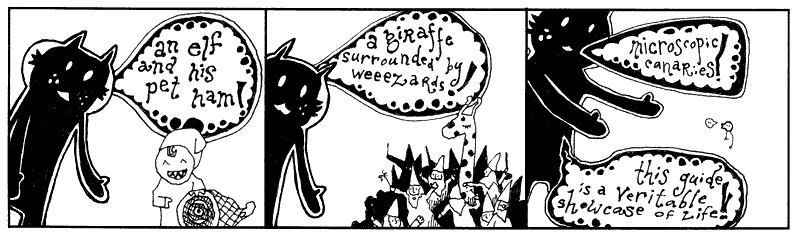
\includegraphics[width=1.0\textwidth]{cache/1.png} 

	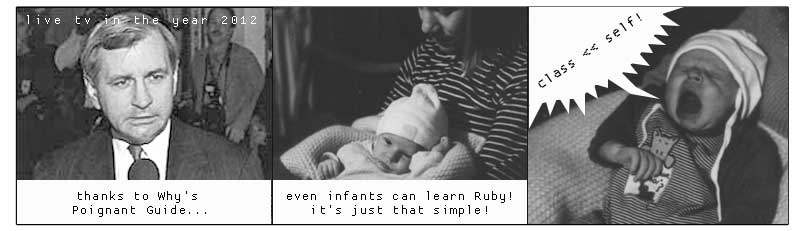
\includegraphics[width=1.0\textwidth]{cache/2.png} 

	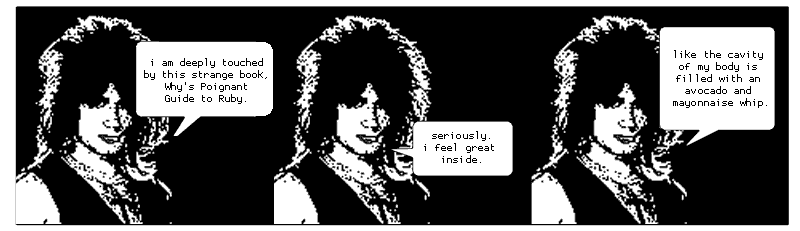
\includegraphics[width=1.0\textwidth]{cache/3.png} 

	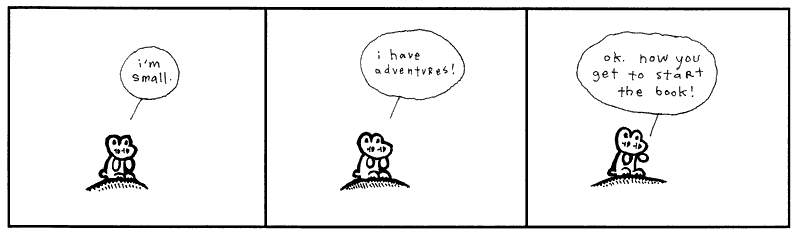
\includegraphics[width=1.0\textwidth]{cache/4.png} 

\newpage
\thispagestyle{empty}
\mbox{}
\cleartooddpage


\chapter{Kon'nichi wa, Ruby}
\vfill
\begin{center}
  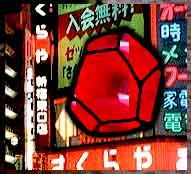
\includegraphics{cache/chapterpoignantguide2.png}
\end{center}
\vspace{2cm}
\newpage
\thispagestyle{empty}
\mbox{}
\clearpage

\section{Opening This Book}

Pretend that you've opened this book (although you probably {\em have}
opened this book), just to find a huge onion right in the middle
crease of the book.  (The manufacturer of the book has included the
onion at my request.)

So you're like, ``Wow, this book comes with an onion!''  (Even if you
don't particularly like onions, I'm sure you can appreciate the
logistics of shipping any sort of produce discreetly inside of an
alleged programming manual.)

Then you ask yourself, ``Wait a minute.  I thought this was a book on
Ruby, the incredible new programming language from Japan.  And
although I can appreciate the logistics of shipping any sort of
produce discreetly inside of an alleged programming manual: Why an
onion? What am I supposed to do with it?''

No.  Please don't puzzle over it.  You don't need to do anything with
the onion.  Set the onion aside and let {\em it} do something with
{\em you}.

I'll be straight with you.  I want you to cry.  To weep.  To whimper
sweetly.  This book is a {\bf poignant} guide to Ruby.  That means
code so beautiful that tears are shed.  That means gallant tales and
somber truths that have you waking up the next morning in the arms of
this book.  Hugging it tightly to you all the day long. If necessary,
fashion a makeshift hip holster for {\em Why's (Poignant) Guide to
  Ruby}, so you can always have this book's tender companionship.

You really must sob once.  Or at least sniffle.  And if not, then the
onion will make it all happen for you.


\section{The Dog Story}


So try this first bit of poignancy on for size:

One day I was walking down one of those busy roads covered with car
dealerships (this was shortly after my wedding was called off) and I
found an orphaned dog on the road.  A wooly, black dog with greenish
red eyes.  I was kind of feeling like an orphan myself, so I took a
couple balloons that were tied to a pole at the dealership and I
relocated them to the dog's collar.  Then, I decided he would be my
dog.  I named him Bigelow.

	\begin{sidebar}{What I'm Going to Do With the Massive Proceeds from this Book}{39}
	Anyone who's written a book can tell you how easily an author is distracted by visions of grandeur. In my experience, I stop twice for each paragraph, and four times for each panel of a comic, just to envision the wealth and prosperity that this book will procure for my lifestyle. I fear that the writing of this book will halt altogether to make way for the armada of SUVs and luxury town cars that are blazing away in my head.\vspace{6pt}

	Rather than stop my production of the (Poignant) Guide, I've reserved this space as a safety zone for pouring my empty and vain wishes.\vspace{6pt}

	Today I was at this Italian restaurant, Granado's, and I was paying my bill. Happened to notice (under glass) a bottle of balsamic vinegar going for \$150. Fairly small. I could conceal it in my palm. Aged twenty-two years.\vspace{6pt}

	I've spent a lot of time thinking about that bottle. It is often an accessory in some of these obsessive fantasies. In one fantasy, I walk into the restaurant, toss a stack of greenery on the counter and earnestly say to the cashier, ``Quick! I have an important salad to make!" \textit{(cont'd)}
	\end{sidebar}

We set off to get some Milkbones for Bigelow and, afterwards, head
over to my place, where we could sit in recliners and listen to
Gorky's Zygotic Mynci.  Oh, and we'd also need to stop by a thrift
store and get Bigelow his own recliner.

But Bigelow hadn't accepted me as his master.  So five minutes later,
the stupid dog took a different crosswalk than I did and I never
caught up.  So whereas he had previously only been lost once, he was
now lost twice.  I slowed my pace towards the life of Milkbones and an
extra recliner.  I had a dog for five minutes.

Stupid Benedict Arnold of a dog.  I sat on a city bench and threw
pinecones at a statue of three sheep crossing a bridge.  After that, I
wept for hours.  The tears just came.  Now there's a little something
poignant to get you started.

I wonder where he went with all those balloons.  That crazy dog must
have looked like a party with legs.

It wasn't much later that I pulled my own Bigelow.  I printed out a
bunch of pages on Ruby.  Articles found around the Web.  I scanned
through them on a train ride home one day.  I flipped through them for
five minutes and then gave up.  Not impressed.

I sat, staring out the window at the world, a life-sized blender
mixing graffiti and iron smelts before my eyes.  {\em This world's too
  big for such a a little language}, I thought. {\em Poor little thing
  doesn't stand a chance.  Doesn't have legs to stand on.  Doesn't
  have arms to swim.}

And yet, there I was.  One little man on a flimsy little train (and I
even still had a baby tooth to lose at the time) out of billions of
people living on a floating blue rock.  How can I knock Ruby?  Who's
to say that I'm not going to happen to choke on my cell phone and die
later that evening.  Why's dead, Ruby lives on.

	\begin{sidebar}{What I'm Going to Do With the Massive Proceeds from this Book}{59}
	\textit{(cont'd)} In another, related fantasy, I am throwing away lettuce. Such roughage isn't befitting of my new vinegar. No, I will have come to a point where the fame and the aristocracy will have corrupted me to my core. My new lettuce will be cash. Cold, hard cash, Mrs. Price.\vspace{6pt}
	
	Soon, I will be expending hundreds for a block of myzithra cheese.\vspace{6pt}

	My imaginations have now gone beyond possessions, though. Certainly, I have thought through my acquisition of Grecian urns, motorcades, airlines, pyramids, dinosaur bones. Occasionally I'll see wind-tossed cities on the news and I'll jot down on my shopping list: \textit{Hurricane}.\vspace{6pt}

	But, now I'm seeing a larger goal. Simply put: what if I amassed such a fortune that the mints couldn't print enough to keep up with my demand? So, everyone else would be forced to use Monopoly money as actual currency. And you would have to win in Monopoly to keep food on the table. These would be some seriously tense games. I mean you go to mortgage St. James Place and your kids start crying. In addition, I think you'll begin to see the end of those who choose to use the Free Parking square as the underground coffers for city funds. \textit{(cont'd)}
	\end{sidebar}

The gravestone:

\begin{quote}
What's in his trachea? Oh, look, a Nokia!
\end{quote}

Just my luck.  Finally get to have a good, long sleep underground,
only to be constantly disturbed by {\em Pachelbel's Canon} going off
in my stomach.


\section{The Red Sun Rises}


So, now you're wondering why I changed my mind about Ruby.  The quick
answer is: we clicked.

Like when you meet Somebody in college and they look like somebody who
used to hit you in the face with paintbrushes when you were a kid.
And so, impulsively, you conclude that this new Somebody is likely a
non-friend.  You wince at their hair.  You hang up phones loudly
during crucial moments in their anecdotes.  You use your pogo stick
right there where they are trying to walk!

Six months later, somehow, you and Somebody are sitting at a fountain
having a perfectly good chat.  Their face doesn't look so much like
that childhood nemesis.  You've met the Good Twin.  You clicked.

So whereas I should probably be pounding your teeth in with hype about
Ruby and the tightly-knit cadre of pertinent ancronyms that accompany
it everywhere (whetting the collective whistles of your bosses and
their bosses' bosses), instead I will just let you coast.  I'll let
you freefall through some code, interjecting occassionally with my own
heartfelt experiences.  It'll be quite easy, quite natural.

I should offer you some sort of motivation, though.  So, Smotchkkiss,
I'm going to give my three best reasons to learn Ruby and be done with
it.

\begin{enumerate}
\item {\bf Brain health.}

Vitamin R.  Goes straight to the head.  Ruby will teach you to {\em
  express} your ideas through a computer.  You will be writing stories
for a machine.

 

Creative skills, people.  Deduction.  Reason.  Nodding
intelligently. The language will become a tool for you to better
connect your mind to the world. I've noticed that many experienced
users of Ruby seem to be clear thinkers and objective.  (In contrast
to: heavily biased and coarse.)


\item {\bf One man on one island.}

Ruby was born in Japan.  Which is freaky.  Japan is not known for its
software.  And since programming languages are largely written in
English, who would suspect a language to come from Japan?

 

And yet, here we have Ruby.  Against the odds, Yukihiro Matsumoto
created Ruby on February 24, 1993.  For the past ten years, he has
steadily brought Ruby to a global audience.  It's triumphant and noble
and all that.  Support diversity. Help us tilt the earth just a bit.


\item {\bf Free.}

Using Ruby costs nothing.  The code to Ruby itself is open for all of
the world to inhale/exhale.  Heck, this book is free.  It's all part
of a great, big giveaway that should have some big hitch to it.

 

You'd think we'd make you buy vacuums or timeshare or fake
Monets. You'd think there'd be a 90 minute presentation where the
owner of the company comes out at the end and knuckles you into
sealing the deal.

 

Nope, free.


\end{enumerate}

With that, it's time for the book to begin.  You can now get out your
highlighter and start dragging it along each captivating word from
this sentence on.  I think I have enough hairspray and funny money on
my person to keep me sustained until the final page.
	
\section{How Books Start}

	\begin{sidebar}{What I'm Going to Do With the Massive Proceeds from this Book}{39}
	\textit{(cont'd)} You've got to hand it to fun money, though. Fake money rules. You can get your hands on it so quickly. For a moment, it seems like you're crazy rich. When I was a kid, I got with some of the neighborhood kids and we built this little Tijuana on our street. We made our own pesos and wore sombreros and everything!\vspace{6pt}
	
	One kid was selling hot tamales for two pesos each. \textit{Two pesos!} Did this kid know that the money was fake? Was he out of his mind? Who invited this kid? Didn't he know this wasn't really Tijuana? Maybe he was really from Tijuana! Maybe these were \textit{real} pesos! Let's go make more \textit{real} pesos!\vspace{6pt}
	
	I think we even had a tavern where you could get totally hammered off Kool-Aid. There's nothing like a bunch of kids stumbling around, mumbling incoherently with punchy red clown lips.
	\end{sidebar}

Now, if you ever have read a book, you know that no book can properly
start without an exorbitant amount of synergy.  Yes, synergy.  Maybe
you didn't know this.  Synergy means that you and I are supposed to
cooperate to make this a great reading experience.

We start off the book by getting along well in the Introduction.  This
togetherness, this {\bf synergy}, propels us through the book, with me
guiding you on your way.  You give me a reassuring nod or snicker to
indicate your progress.

I'm Peter Pan holding your hand.  Come on, Wendy!  Second star to the
right and on till morning.

One problem here.  I don't get along well with people.  I don't hold
hands very well.

Any of my staff will tell you.  At the Opening Ceremonies of This Book
(a catered event with stadium seating), I discovered that the cucumber
sandwiches weren't served in tea towels. As a result, the butter
hadn't set with the cucumbers right... Anyways, I made a big scene and
set fire to some of the advertising trucks outside.  I smashed this
spotlight to pieces and so on.  I had this loud maniacal laughing
thing going on deep into that night.  It was a real mess.

But, since I don't get along well with people, I hadn't invited anyone
but myself to the Opening Ceremonies of This Book.  So it wasn't
really that embarassing.  I kept it under wraps and no one found out
about the whole ordeal.

So you've got to know that {\bf synergy} doesn't actually mean {\bf
  synergy} in this book.  I can't do normal {\bf synergy}. No, in this
book, {\bf synergy} means {\bf cartoon foxes}.  What I'm saying is:
this book will be starting off with an exorbitant amount of {\bf
  cartoon foxes}.

And I will be counting on you to turn them into {\bf synergy}.

\newpage
\thispagestyle{empty}
\mbox{}

\cleartooddpage

\chapter{A Quick (and Hopefully Painless) Ride Through Ruby \mbox{(with Cartoon Foxes)}}
\vfill
\begin{center}
  
\includegraphics{cache/chapterpoignantguide3.png}
\end{center}
\vspace{2cm}
\newpage
\thispagestyle{empty}
\mbox{}
\clearpage

	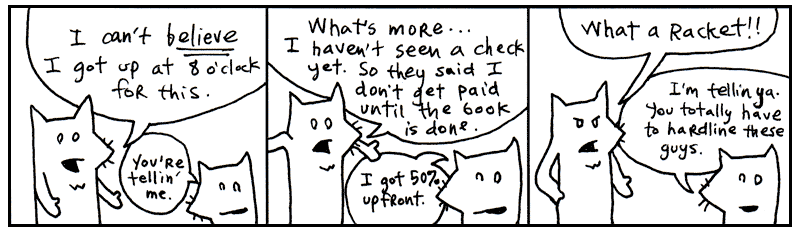
\includegraphics[width=1.0\textwidth]{cache/5.png}

Yeah, these are the two.  My asthma's kickin in so I've got to go take
a puff of medicated air just now.  Be with you in a moment.

	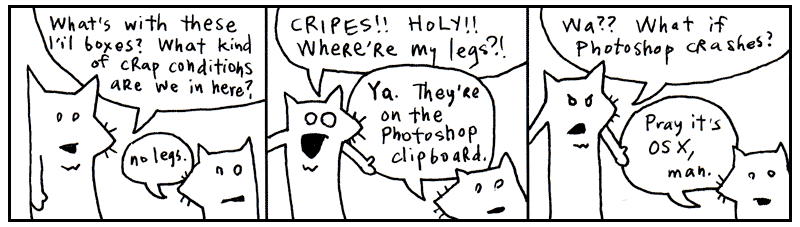
\includegraphics[width=1.0\textwidth]{cache/6.png}

I'm told that this chapter is best accompanied by a rag.  Something
you can mop your face with as the sweat pours off your face.

Indeed, we'll be racing through the whole language.  Like striking
every match in a box as quickly as can be done.


\section{Language and I MEAN Language}

	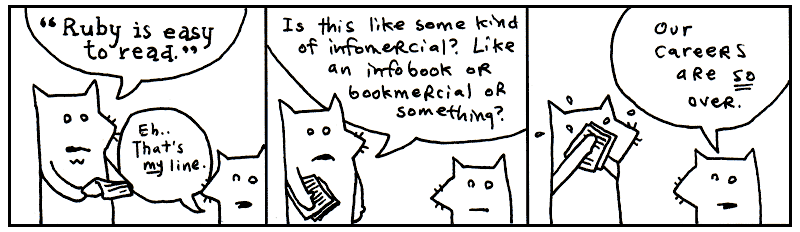
\includegraphics[width=1.0\textwidth]{cache/7.png}

My conscience won't let me call Ruby a {\em computer} language.  That
would imply that the language works primarily on the computer's terms.
That the language is designed to accomodate the computer, first and
foremost.  That therefore, we, the coders, are foreigners, seeking
citizenship in the computer's locale.  It's the computer's language
and we are translators for the world.

But what do you call the language when your brain begins to think in
that language?  When you start to use the language's own words and
colloquialisms to express yourself.  Say, the computer can't do that.
How can it be the computer's language?  It is ours, we speak it
natively!

We can no longer truthfully call it a {\em computer} language.  It is
{\em coderspeak}.  It is the language of our thoughts.

{\bf Read the following aloud to yourself.}

\begin{quote}
\lstinline[breaklines=true]|5.times { print "Odelay!" }|\end{quote}


In English sentences, punctuation (such as periods, exclamations,
parentheses) are silent.  Punctuation adds meaning to words, helps
give cues as to what the author intended by a sentence.  So let's read
the above as: {\em Five times print ``Odelay!''.}

Which is exactly what this small Ruby program does.  Beck's mutated
Spanish exclamation will print five times on the computer screen.

\newpage

{\bf Read the following aloud to yourself.}

\begin{quote}
\lstinline[breaklines=true]|exit unless "restaurant".include? "aura"|\end{quote}


Here we're doing a basic reality check.  Our program will {\bf exit}
(the program will end) {\bf unless} the word {\bf restaurant} contains
(or {\bf includes}) the word {\bf aura}.  Again, in English: {\em Exit
  unless the word restaurant includes the word aura.}

Ever seen a programming language use question marks so effectively?
Ruby uses some punctuation, such as exclamations and question marks,
to enhance readability of the code.  We're asking a question in the
above code, so why not make that apparent?

{\bf Read the following aloud to yourself.}

\begin{quote}
\lstinline[breaklines=true]$['toast', 'cheese', 'wine'].each { |food|  print food.capitalize }$\end{quote}


While this bit of code is less readable and sentence-like than the
previous examples, I'd still encourage you to read it aloud.  While
Ruby may sometimes read like English, it sometimes reads as a shorter
English.  Fully translated into English, you might read the above as:
{\em With the words `toast', `cheese', and `wine': take each food and
  print it capitalized.}

The computer then courteously responds:
\lstinline[breaklines=true]|Toast|,
\lstinline[breaklines=true]|Cheese| and
\lstinline[breaklines=true]|Wine|.

At this point, you're probably wondering how these words actually fit
together.  Smotchkkiss is wondering what the dots and brackets mean.
I'm going to discuss the various {\em parts of speech} next.

All you need to know thus far is that Ruby is basically built from
sentences.  They aren't exactly English sentences.  They are short
collections of words and punctuation which encompass a single thought.
These sentences can form books.  They can form pages.  They can form
entire novels, when strung together. Novels that can be read by
humans, but also by computers.


\section{The Parts of Speech}


Just like the white stripe down a skunk's back and the winding, white
train of a bride, many of Ruby's parts of speech have visual cues to
help you identify them.  Punctuation and capitalization will help your
brain to see bits of code and feel intense recognition. Your mind will
frequently yell {\em Hey, I know that guy!}  You'll also be able to
name-drop in conversations with other Rubyists.

	\begin{sidebar}{Concerning Commercial Uses of the (Poignant) Guide}{100}
		This book is released under a Creative Commons license which allows unlimited commercial use of this text. Basically, this means you can sell all these bootleg copies of my book and keep the revenues for yourself. I trust my readers (and the world around them) to rip me off. To put out some crappy Xerox edition with that time-tested clipart of praying hands on the cover.\vspace{6pt}
		
		Guys, the lawsuits just ain't worth the headache. So I'm just going to straight up endorse authorized piracy, folks. Anybody who wants to read the book should be able to read it. Anybody who wants to market the book or come up with special editions, I'm flattered.\vspace{6pt}
		
		Why would I want the \$\$\$? IGNORE ALL OTHER SIDEBARS: I've lost the will to be a rich slob. Sounds inhuman, but I like my little black-and-white television. Also my hanging plastic flower lamp. I don't want to be a career writer. Cash isn't going inspire me. Pointless.\vspace{6pt}
		
		So, if money means nothing to the lucky stiff, why rip me off when you could co-opt shady business practices to literally crush my psyche and leave me wheezing in some sooty iron lung? Oh, and the irony of using my own works against me! Die, Poignant Boy! \textit{(cont'd)}
	\end{sidebar}

Try to focus on the look of each of these parts of speech.  The rest
of the book will detail the specifics.  I give short descriptions for
each part of speech, but you don't have to understand the explanation.
By the end of this chapter, you should be able to recognize every part
of a Ruby program.



\subsection{Variables}



Any plain, lowercase word is a variable in ruby.  Variables may
consist of letters, digits and underscores.

\begin{quote}
\lstinline[breaklines=true]|x|, \lstinline[breaklines=true]|y|,
\lstinline[breaklines=true]|banana2| or
\lstinline[breaklines=true]|phone_a_quail| are examples.\end{quote}


Variables are like nicknames.  Remember when everyone used to call you
Stinky Pete? People would say, ``Get over here, Stinky Pete!''  And
everyone miraculously knew that Stinky Pete was you.

With variables, you give a nickname to something you use frequently.
For instance, let's say you run an orphanage.  It's a mean orphanage.
And whenever Daddy Warbucks comes to buy more kids, we insist that he
pay us {\bf one-hundred twenty-one dollars and eight cents} for the
kid's teddy bear, which the kid has become attached to over in the
darker moments of living in such nightmarish custody.

\begin{quote}
\lstinline[breaklines=true]|teddy_bear_fee = 121.08|\end{quote}


Later, when you ring him up at the cash register (a really souped-up
cash register which runs Ruby!), you'll need to add together all his
charges into a {\bf total}.

\begin{quote}
\lstinline[breaklines=true]|total = orphan_fee + teddy_bear_fee + gratuity|\end{quote}

Those variable nicknames sure help.  And in the seedy underground of
child sales, any help is appreciated I'm sure.

	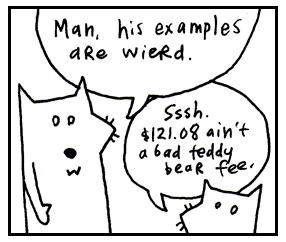
\includegraphics[width=0.3575\textwidth]{cache/8.png}

\subsection{Numbers}



The most basic type of number is an {\em integer}, a {\bf series of
  digits} which can start with a {\bf plus or minus sign}.

\begin{quote}
\lstinline[breaklines=true]|1|, \lstinline[breaklines=true]|23|, and
\lstinline[breaklines=true]|-10000| are examples.\end{quote}


Commas are not allowed in numbers, but underscores are.  So if you
feel the need to mark your thousands so the numbers are more readable,
use an underscore.

\begin{quote}
\lstinline[breaklines=true]|population = 12_000_000_000|\end{quote}


Decimal numbers are called {\em floats} in Ruby.  Floats consist of
numbers with {\bf a decimal place} or {\bf scientific notation}.

\begin{quote}
\lstinline[breaklines=true]|3.14|,
\lstinline[breaklines=true]|-808.08| and
\lstinline[breaklines=true]|12.043e-04| are examples.\end{quote}





\subsection{Strings}



Strings are any sort of characters (letters, digits, punctuation)
surrounded by quotes.  Both single and double {\bf quotes} are used to
create strings.

	\begin{sidebar}{Concerning Commercial Uses of the (Poignant) Guide}{250}
		\textit{(cont'd) }To give you an idea of what I mean, here are a few underhanded concepts that could seriously kill my willpower and force me to reconsider things like existence.\vspace{6pt}
		
		\textbf{IDEA ONE: BIG TOBACCO}\vspace{6pt}
		
		Buy a cigarette company. Use my cartoon foxes to fuel an aggressive ad campaign. Here's a billboard for starters:\vspace{6pt}
	
		\hfill
		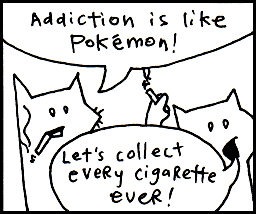
\includegraphics[width=0.8\textwidth]{cache/sidebar311.png}
		\hspace*{\fill}
		
		Make it obvious that you're targeting children and the asthmatic. Then, once you've got everyone going, have the truth people do an expose on me and my farm of inky foxes.\vspace{6pt}
		
		\begin{quoting}[rightmargin=0pt,leftmargin=0.5\leftmargin,font=itshape]
			\textbf{Sensible Hipster Standing on Curb in Urban Wilderness}: He calls himself the lucky stiff.\vspace{4pt}
			
			{\scriptsize (Pulls aside curtain to reveal gray corpse on a gurney.)}\vspace{4pt}
			
			\textbf{Hipster}: Some stiffs ain't so lucky.\vspace{4pt}
			
			{\scriptsize (Erratic zoom in. Superimposed cartoon foxes for subliminal Willy Wonka mind trip.) }
		\end{quoting}
		
		\hfill\textit{(cont'd)}
	\end{sidebar}

\begin{quote}
\lstinline[breaklines=true]|"sealab"|,
\lstinline[breaklines=true]|'2021'|, or
\lstinline[breaklines=true]|"These cartoons are hilarious!"| are
examples.\end{quote}


When you enclose characters in quotes, they are stored together as a
single string.

Think of a reporter who is jotting down the mouthnoises of a rambling
celebrity.  ``I'm a lot wiser,'' says Avril Lavigne.  ``Now I know
what the business is like -- what you have to do and how to work it.''


\begin{lstlisting}[basicstyle=\ttfamily\color{basiccolor},
    commentstyle = \ttfamily\color{commentcolor},
    keywordstyle=\ttfamily\color{keywordscolor},
    stringstyle=\color{stringcolor},
    language=Ruby,
    basicstyle=\small\ttfamily,
    showstringspaces=false,
  ]

  avril_quote = "I'm a lot wiser.  Now I know
  what the business is like -- what you have
  to do and how to work it."

\end{lstlisting}


So, just as we stored a number in the {\bf teddy\_bear\_fee} variable,
now we're storing a collection of characters (a string) in the {\bf
  avril\_quote} variable.  The reporter sends this quote to the
printers, who just happen to use Ruby to operate their printing press.


\begin{lstlisting}[basicstyle=\ttfamily\color{basiccolor},
    commentstyle = \ttfamily\color{commentcolor},
    keywordstyle=\ttfamily\color{keywordscolor},
    stringstyle=\color{stringcolor},
    language=Ruby,
    basicstyle=\small\ttfamily,
    showstringspaces=false,
  ]

 print oprah_quote
 print avril_quote
 print ashlee_simpson_debacle

\end{lstlisting}

	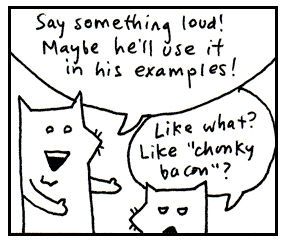
\includegraphics[width=0.3575\textwidth]{cache/9.png}


\pagebreak
\subsection{Symbols}

	\begin{sidebar}{Concerning Commercial Uses of the (Poignant) Guide}{240}
		\textit{(cont'd)} Yo. Why you gotta dis Big Smokies like dat, Holmes?\vspace{6pt}
		
		\textbf{IDEA TWO: HEY, FIRING SQUAD}\vspace{6pt}
		
		Like I said, start selling copies of my book, but corrupt the text. These altered copies would contain numerous blatant (and libelous) references to government agencies, such as the U.S. Marshals and the Pentagon. You could make me look like a complete traitor. Like I have all these plans to, you know, kill certain less desirable members of the U.S. Marshals or the Pentagon.\vspace{6pt}
		
		Not that there are any less desirable members of the U.S. Marshals or the Pentagon. Yeah, I didn't mean it like that.\vspace{6pt}
		
		Oh, crap.\vspace{6pt}
		
		Oh, crap. Oh, crap. Oh, crap.\vspace{6pt}
		
		Turn off the lights. Get down.\vspace{6pt}
		
		\textbf{IDEA THREE: BILLBOARDS, PART II}\vspace{6pt}
		
		How about making fun of asthmatics directly?\vspace{6pt}
		
		\hfill
		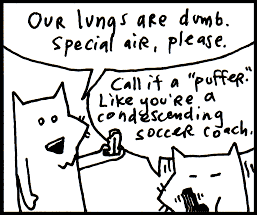
\includegraphics[width=0.8\textwidth]{cache/sidebar312.png}
		\hspace*{\fill}
		
		\textit{(cont'd)}
	\end{sidebar}

Symbols are words that look just like variables.  Again, they may
contain letters, digits, or underscores.  But they {\bf start with a
  colon}.

\begin{quote}
\lstinline[breaklines=true]|:a|, \lstinline[breaklines=true]|:b|, or
\lstinline[breaklines=true]|:ponce_de_leon| are examples.\end{quote}


Symbols are lightweight strings.  Usually, symbols are used in
situations where you need a string but you won't be printing it to the
screen.

You could say a symbol is a bit easier on the computer.  It's like an
antacid.  The colon indicates the bubbles trickling up from your
computer's stomach as it digests the symbol.  Ah.  Sweet, sweet
relief.

	% moving out of way of sidebar
	\hspace*{1mm}
	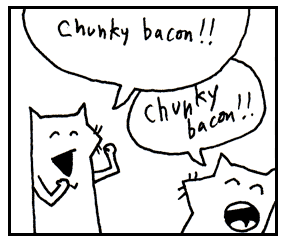
\includegraphics[width=0.3575\textwidth]{cache/10.png}




\subsection{Constants}



Constants are words like variables, but constants are {\bf
  capitalized}.  If variables are the nouns of Ruby, then think of
constants as the proper nouns.

\begin{quote}
\lstinline[breaklines=true]|Time|, \lstinline[breaklines=true]|Array|
or \lstinline[breaklines=true]|Bunny_Lake_is_Missing| are
examples.\end{quote}


	\begin{sidebar}{Concerning Commercial Uses of the (Poignant) Guide}{200}
		\textit{(cont'd)} \textbf{IDEA FOUR: ALEC BALDWIN}\vspace{6pt}
		
		Adapt the book into a movie. And since, you know, I'm a character in this book, you could get someone like Alec Baldwin to play me. Someone who's at a real low point in his career.\vspace{6pt}

		You could make it seem like I did tons of drugs. Like I was insane to work with. Like I kept firing people and locking them in the scooter room and making them wear outfits made of bread. Yeah, like I could actually be baking people into the outfits.\vspace{6pt}

		You could have this huge mold that I strap people into. Then, I pour all the dough on them and actually bake them until the bread has risen and they've almost died. And when the television crews come and I'm on Good Morning America, they'll ask, ``So, how many people have you employed in the production of your book?" And I'd respond, ``A baker's dozen!" and erupt into that loud maniacal laughing that would force audience members to cup their hands over their ears.\vspace{6pt}

		Of course, in the throes of my insanity, I would declare war on the world. The bread people would put up quite a fight. Until the U.S. Marshals (or the Pentagon) engineer a giant robotic monkey brain (played by Burt Lancaster) to come after me. \textit{(cont'd)}
	\end{sidebar}

In English, proper nouns are capitalized.  The Empire State Building.
You can't just move The Empire State Building.  You can't just decide
that the Empire State Building is something else. Proper nouns are
like that.  They refer to something very specific and usually don't
change over time.

In the same way, constants can't be changed after they are set.

\begin{quote}
\lstinline[breaklines=true]|EmpireStateBuilding = "350 5th Avenue, NYC, NY"|\end{quote}


If we try to change the constant, Ruby will complain to us.  Such
things are frowned upon.

	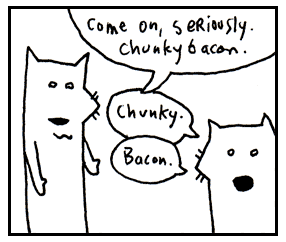
\includegraphics[width=0.3575\textwidth]{cache/11.png}




\subsection{Methods}



If variables and constants are the nouns, then methods are the
verbs. Methods are usually attached to the end of variables and
constants by a {\bf dot}.  You've already seen methods at work.

\begin{quote}
\lstinline[breaklines=true]|front_door.open|\end{quote}


In the above, {\bf open} is the method.  It is the action, the
verb. In some cases, you'll see actions chained together.

\begin{quote}
\lstinline[breaklines=true]|front_door.open.close|\end{quote}

	\begin{sidebar}{Concerning Commercial Uses of the (Poignant) Guide}{100}
		\textit{(cont'd)}Here's where you'll make me look completely lame. Not only will I sacrifice all of the bread people (the Starchtroopers) to save myself, not only will I surrender to the great monkey brain like a coward, but when I narrowly escape, I'll yell at the audience. Screaming insistently that it's MY movie and no one should see it any more, I'll rip the screen in half and the film projector will spin with its reel flapping in defeat. And that will be the end of the movie. People will be so pissed.\vspace{6pt}

		Now, I've got to thinking. See, and actually, Alec Baldwin did a decent voiceover in \textit{The Royal Tenenbaums}. His career might be okay. You might not want to use him. He might not do it.\vspace{6pt}

		Tell ya what. I'll play the part. I've made a career out of low points.
	\end{sidebar}

We've instructed the computer to open the front door and then
immediately close it.

\begin{quote}
\lstinline[breaklines=true]|front_door.is_open?|\end{quote}


The above is an action as well.  We're instructing the computer to
test the door to see if it's open. The method could be called
\lstinline[breaklines=true]|Door.test_to_see_if_its_open|, but the
\lstinline[breaklines=true]|is_open?| name is succinct and just as
correct.  Both exclamation marks and question marks may be used in
method names.



\subsection{Method arguments}



A method may require more information in order to perform its action.
If we want the computer to paint the door, we should provide a color
as well.

Method arguments are attached to the end of a method.  The arguments
are usually surrounded by {\bf parentheses} and separated by {\bf
  commas}.

\begin{quote}
\lstinline[breaklines=true]|front_door.paint( 3, :red )|\end{quote}


The above paints the front door 3 coats of red.

Think of it as an inner tube the method is pulling along, containing
its extra instructions. The parentheses form the wet, round edges of
the inner tube.  The commas are the feet of each argument, sticking
over the edge.  The last argument has its feet tucked under so they
don't show.

Like a boat pulling many inner tubes, methods with arguments can be
chained.

\begin{quote}
\lstinline[breaklines=true]|front_door.paint( 3, :red ).dry( 30 ).close()|\end{quote}


The above paints the front door 3 coats of red, dries for 30 minutes,
and closes the door.  Even though the last method has no arguments,
you can still put parentheses if you like.  There is no use dragging
an empty inner tube, so the parentheses are normally dropped.

Some methods (such as \lstinline[breaklines=true]|print|) are kernel
methods.  These methods are used throughout Ruby.  Since they are so
common, you won't use the dot.

\begin{quote}
\lstinline[breaklines=true]|print "See, no dot."|\end{quote}




\subsection{Class methods}



Like the methods described above (also called {\em instance} methods),
class methods are usually attached after variables and constants.
Rather than a dot, a {\bf double colon} is used.

\begin{quote}
\lstinline[breaklines=true]|Door::new( :oak )|\end{quote}


As seen above, the \lstinline[breaklines=true]|new| class method is
most often used to create things.  In the above example, we're asking
Ruby to make a new oak door for us.  Of course, Ruby has to have an
understanding of how to make a door--as well as a wealth of timber,
lumberjacks, and those long, wiggily, two-man saws.

	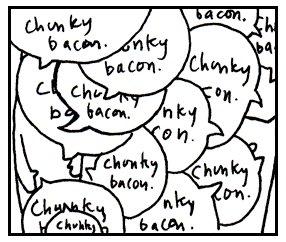
\includegraphics[width=0.3575\textwidth]{cache/12.png}




\subsection{Global variables}



Variables which begin with a {\bf dollar sign} are global.

\begin{quote}
\lstinline[breaklines=true]|$x|, \lstinline[breaklines=true]|$1|,
\lstinline[breaklines=true]|$chunky| and
\lstinline[breaklines=true]|$CHunKY_bACOn| are examples.\end{quote}


Most variables are rather temporary in nature.  Some parts of your
program are like little houses. You walk in and they have their own
variables.  In one house, you may have a
\lstinline[breaklines=true]|dad| that represents Archie, a travelling
salesman and skeleton collector.  In another house,
\lstinline[breaklines=true]|dad| could represent Peter, a lion tamer
with a great love for flannel.  Each house has its own meaning for
\lstinline[breaklines=true]|dad|.

With global variables, you can be guaranteed that the variable is the
same in every little house. The dollar sign is very appropriate.
Every American home respects the value of the dollar.  We're crazy for
the stuff.  Try knocking on any door in America and hand them cash.  I
can guarantee you won't get the same reaction if you knock on a door
and offer Peter, a lion tamer with a great love for flannel.

Global variables can be used anywhere in your program.  They never go
out of sight.




\subsection{Instance variables}



Variables which begin with an {\bf at} symbol are instance variables.

\begin{quote}
\lstinline[breaklines=true]|@x|, \lstinline[breaklines=true]|@y|, and
\lstinline[breaklines=true]|@only_the_chunkiest_cut_of_bacon_I_have_ever_seen|
are examples.\end{quote}


These variables are often used to define the attributes of something.
For example, you might provide Ruby with the width of the
\lstinline[breaklines=true]|front_door| by setting the
\lstinline[breaklines=true]|@width| variable inside that
\lstinline[breaklines=true]|front_door|.  Instance variables are used
to define characteristics of a single object in Ruby.

Think of the {\bf at} symbol as meaning {\bf attribute}.




\subsection{Class variables}



Variables which begin with {\bf double at} symbols are class
variables.

\begin{quote}
\lstinline[breaklines=true]|@@x|, \lstinline[breaklines=true]|@@y|,
and
\lstinline[breaklines=true]|@@i_will_take_your_chunky_bacon_and_raise_you_two|
are examples.\end{quote}


Class variables, too, are used to define attributes.  But rather than
defining an attribute for a single object in Ruby, class variables
give an attribute to many related objects in Ruby.  If instance
variables set attributes for a single
\lstinline[breaklines=true]|front_door|, then class variables set
attributes for everything that is a \lstinline[breaklines=true]|Door|.

Think of the {\bf double at} prefix as meaning {\bf attribute all}.
Additionally, you can think of a swarm of {\bf AT-ATs} from {\em Star
  Wars}, which are all commanded by Ruby.  You change a class variable
and not just one changes, they all change.

	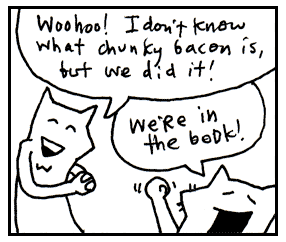
\includegraphics[width=0.3575\textwidth]{cache/13.png}




\subsection{Blocks}



Any code surrounded by {\bf curly braces} is a block.

\begin{quote}
\lstinline[breaklines=true]|2.times { print "Yes, I've used chunky bacon in my examples, but never again!" }| is an example.\end{quote}


With blocks, you can group a set of instructions together so that they
can be passed around your program.  The curly braces give the
appearance of crab pincers that have snatched the code and are holding
it together.  When you see these two pincers, remember that the code
inside has been pressed into a single unit.

It's like one of those little Hello Kitty boxes they sell at the mall
that's stuffed with tiny pencils and microscopic paper, all crammed
into a glittery transparent case that can be concealed in your palm
for covert stationary operations.  Except that blocks don't require so
much squinting.

The curly braces can also be traded for the words {\bf do} and {\bf
  end}, which is nice if your block is longer than one line.


\begin{lstlisting}[basicstyle=\ttfamily\color{basiccolor},
    commentstyle = \ttfamily\color{commentcolor},
    keywordstyle=\ttfamily\color{keywordscolor},
    stringstyle=\color{stringcolor},
    language=Ruby,
    basicstyle=\small\ttfamily,
    showstringspaces=false,
  ]

 loop do
   print "Much better."
   print "Ah.  More space!"
   print "My back was killin' me in those crab pincers."
 end

\end{lstlisting}





\subsection{Block arguments}



Block arguments are a set of variables surrounded by {\bf pipe}
characters and separated by {\bf commas}.

\begin{quote}
\lstinline[breaklines=true]$|en||x|$,
\lstinline[breaklines=true]$|x,y|$, and
\lstinline[breaklines=true]$|up, down, all_around|$ are
examples.\end{quote}


Block arguments are used at the beginning of a block.

\begin{quote}
\lstinline[breaklines=true]${ |x,y| x + y }$\end{quote}


In the above example, \lstinline[breaklines=true]$|x,y|$ are the
arguments.  After the arguments, we have a bit of code.  The
expression \lstinline[breaklines=true]|x + y| adds the two arguments
together.

I like to think of the pipe characters as representing a tunnel.  They
give the appearance of a chute that the variables are sliding down.
(An \lstinline[breaklines=true]|x| goes down spread eagle, while the
\lstinline[breaklines=true]|y| neatly crosses her legs.)  This chute
acts as a passageway between blocks and the world around them.

Variables are passed through this chute (or tunnel) into the block.

	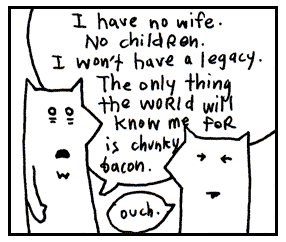
\includegraphics[width=0.3575\textwidth]{cache/14.png}




\subsection{Ranges}



A range is two values surrounded by {\bf parentheses} and separated by
{\bf an ellipsis} (in the form of two or three dots).

\begin{quote}
\lstinline[breaklines=true]|(1..3)| is a range, representing the
numbers 1 through 3.\end{quote}


\begin{quote}
\lstinline[breaklines=true]|('a'..'z')| is a range, representing a
lowercase alphabet.\end{quote}


Think of it as an accordion which has been squeezed down for carrying.
(Sure, you can build a great sense of self-worth by carrying around an
unfolded accordion, but sometimes a person needs to wallow in
self-doubt, carefully concealing the squeeze-box.)  The parentheses
are the handles on the sides of a smaller, handheld accordion.  The
dots are the chain, keeping the folds tightly closed.

Normally, only two dots are used.  If a third dot is used, the last
value in the range is excluded.

\begin{quote}
\lstinline[breaklines=true]|(0...5)| represents the numbers 0 through
4.\end{quote}


When you see that third dot, imagine opening the accordion slightly.
Just enough to let one note from its chamber.  The note is that end
value.  We'll let the sky eat it.



\subsection{Arrays}



An array is a list surrounded by {\bf square brackets} and separated
by {\bf commas}.

\begin{quote}
\lstinline[breaklines=true]|[1, 2, 3]| is an array of
numbers.\end{quote}


\begin{quote}
\lstinline[breaklines=true]|['coat', 'mittens', 'snowboard']| is an
array of strings.\end{quote}


Think of it as a caterpillar which has been stapled into your code.
The two square brackets are staples which keep the caterpillar from
moving, so you can keep track of which end is the head and which is
the tail.  The commas are the caterpillar's legs, wiggling between
each section of its body.

Once there was a caterpillar who had commas for legs.  Which meant he
had to allow a literary pause after each step.  The other caterpillars
really respected him for it and he came to have quite a commanding
presence.  Oh, and talk about a philanthropist!  He was notorious for
giving fresh leaves to those less-fortunate.

Yes, an array is a collection of things, but it also keeps those
things in a specific order.




\subsection{Hashes}



A hash is a dictionary surrounded by {\bf curly braces}.  Dictionaries
match words with their definitions.  Ruby does so with {\bf arrows}
made from an equals sign, followed by a greater-than sign.

\begin{quote}
\lstinline[breaklines=true]|{'a' => 'aardvark', 'b' => 'badger'}| is
an example.\end{quote}


This time, the curly braces represent little book symbols.  See how
they look like little, open books with creases down the middle?  They
represent opening and closing our dictionary.

Imagine our dictionary has a definition on each of its pages.  The
commas represent the corner of each page, which we turn to see the
next definition.  And on each page: a word followed by an arrow
pointing to the definition.


\begin{lstlisting}[basicstyle=\ttfamily\color{basiccolor},
    commentstyle = \ttfamily\color{commentcolor},
    keywordstyle=\ttfamily\color{keywordscolor},
    stringstyle=\color{stringcolor},
    language=Ruby,
    basicstyle=\small\ttfamily,
    showstringspaces=false,
  ]

 {
   'name' => 'Peter',
   'profession' => 'lion tamer',
   'great love' => 'flannel'
 }

\end{lstlisting}


I'm not comparing hashes to dictionaries because you can only store
definitions in a hash.  In the example above, I stored personal
information for Peter, the lion tamer with a great love for flannel.
Hashes are like dictionaries because they can be very easy to search
through.

Unlike arrays, the items in a hash are not kept in a specific order.

	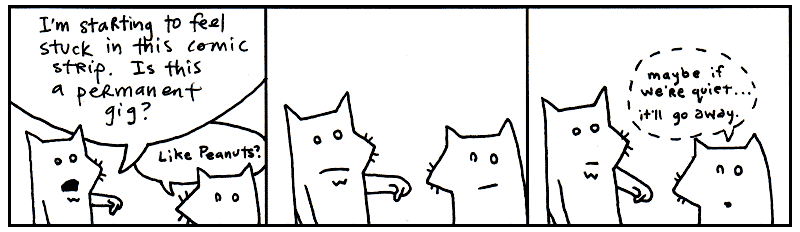
\includegraphics[width=1.0\textwidth]{cache/15.png}




\subsection{Regular Expressions}



A regular expression (or {\em regexp}) is a set of characters
surrounded by {\bf slashes}.

\begin{quote}
\lstinline[breaklines=true]|/ruby/|,
\lstinline[breaklines=true]|/[0-9]+/| and
\lstinline[breaklines=true]|/^\d{3}-\d{3}-\d{4}/| are
examples.\end{quote}


Regular expressions are used to find words or patterns in text.  The
slashes on each side of the expression are pins.

Imagine if you had a little word with pins on both side and you held
it over a book.  You pass the word over the book and when it gets near
a matching word, it starts blinking.  You pin the regular expression
onto the book, right over the match and it glows with the letters of
the matching word.

Oh, and when you poke the pins into the book, the paper sneezes, {\em
  reg-exp!}

Regular expressions are much faster than passing your hand over pages
of a book.  Ruby can use a regular expression to search volumes of
books very quickly.



\subsection{Operators}



You'll use the following list of operators to do math in Ruby or to
compare things. Scan over the list, recognize a few.  You know,
addition \lstinline[breaklines=true]|+| and subtraction
\lstinline[breaklines=true]|-| and so on.


\begin{lstlisting}

  ** !  ~  *  /  %  +  -  & 
  << >> |  ^  >  >= <  <= <=>
  || != =~ !~ && += -= == ===
  .. ... not and or

\end{lstlisting}




\subsection{Keywords}



Ruby has a number of built-in words, imbued with meaning.  These words
cannot be used as variables or changed to suit your purposes.  Some of
these we've already discussed.  They are in the safe house, my friend.
You touch these and you'll be served an official syntax error.


\begin{lstlisting}[basicstyle=\ttfamily\color{basiccolor},
    commentstyle = \ttfamily\color{commentcolor},
    keywordstyle=\ttfamily\color{keywordscolor},
    stringstyle=\color{stringcolor},
    language=Ruby,
    basicstyle=\small\ttfamily,
    showstringspaces=false,
  ]

  alias   and     BEGIN   begin   break   case    class   def     defined 
  do      else    elsif   END     end     ensure  false   for     if 
  in      module  next    nil     not     or      redo    rescue  retry
  return  self    super   then    true    undef   unless  until   when 
  while   yield

\end{lstlisting}


Good enough.  These are the illustrious members of the Ruby language.
We'll be having quite the junket for the next three chapters, gluing
these parts together into sly bits of (poignant) code.

I'd recommend skimming all of the parts of speech once again.  Give
yourself a broad view of them.  I'll be testing your metal in the next
section.

	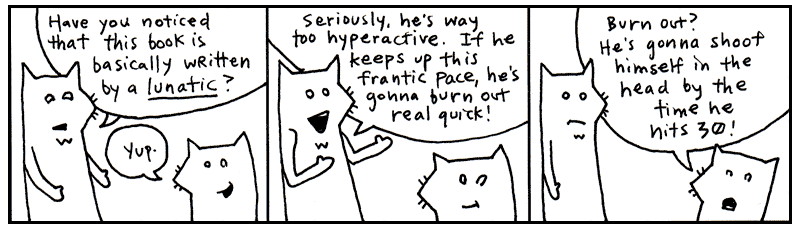
\includegraphics[width=1.0\textwidth]{cache/16.png}


\section{If I Haven't Treated You Like a Child Enough Already}

	\begin{sidebar}{Seven Moments of Zen from My Life}{39}
		\begin{enumerate}
			\item 8 years old. Just laying in bed, thinking. And I realize. \textit{There's nothing stopping me from becoming a child dentist.}
			\item 21. Found a pencil on the beach. Embossed on it: \textit{I cherish serenity}. Tucked it away into the inside breast pocket of my suit jacket. Watched the waves come and recede.
			\item 22. Found a beetle in my bathroom that was just about to fall into a heating vent. Swiped him up. Tailored him a little backpack out of a leaf and a thread. In the backpack: a skittle and a AAA battery. That should last him. Set him loose out by the front gate.
			\item Three years of age. Brushed aside the curtain. Sunlight.
		\end{enumerate}
		\textit{(cont'd)}
	\end{sidebar}

I'm proud of you.  Anyone will tell you how much I brag about you.
How I go on and on about this great anonymous person out there who
scrolls and reads and scrolls and reads.  ``These kids,'' I tell them.
``Man, these kids got heart.  I never...''  And I can't even finish a
sentence because I'm absolutely blubbering.

And my heart glows bright red under my filmy, translucent skin and
they have to administer 10cc of JavaScript to get me to come back.  (I
respond well to toxins in the blood.)  Man, that stuff will kick the
peaches right out your gills!

So, yes.  You've kept up nicely.  But now I must begin to be a brutal
schoolmaster. I need to start seeing good marks from you.  So far,
you've done nothing but move your eyes around a lot.  Okay, sure, you
did some exceptional reading aloud earlier.  Now we need some
comprehension skills here, Smotchkkiss.

{\bf Say aloud each of the parts of speech used below.}

\begin{quote}
\lstinline[breaklines=true]|5.times { print "Odelay!" }|\end{quote}


You might want to even cover this paragraph up while you read, because
your eyes might want to sneak to the answer.  We have a {\em number}
\lstinline[breaklines=true]|5|, followed by a {\em method}
\lstinline[breaklines=true]|.times|.  Then, the first crab pincers of
a {\em block}.  The kernel {\em method}
\lstinline[breaklines=true]|print| has no dot and is followed by a
          {\em string} \lstinline[breaklines=true]|"Odelay!"|.  The
          final crab pincers close our {\em block}.

{\bf Say aloud each of the parts of speech used below.}

\begin{quote}
\lstinline[breaklines=true]|exit unless "restaurant".include? "aura"|\end{quote}


Like the \lstinline[breaklines=true]|print| method,
\lstinline[breaklines=true]|exit| is a kernel {\em method}.  If you
were paying attention during the big list of keywords, you'll know
that \lstinline[breaklines=true]|unless| is just such a {\em keyword}.
The {\em string} \lstinline[breaklines=true]|"restaurant"| is clung to
by the {\em method} \lstinline[breaklines=true]|include?|.  And
finally, the string \lstinline[breaklines=true]|"aura"|.

{\bf Say aloud each of the parts of speech used below.}

\begin{lstlisting}[basicstyle=\ttfamily\color{basiccolor},
    commentstyle = \ttfamily\color{commentcolor},
    keywordstyle=\ttfamily\color{keywordscolor},
    stringstyle=\color{stringcolor},
    language=Ruby,
    basicstyle=\small\ttfamily,
    showstringspaces=false,
  ]

 ['toast', 'cheese', 'wine'].each { 
 	|food| print( food.capitalize ) 
 }

\end{lstlisting}

This caterpillar partakes of finer delicacies.  An {\em array} starts
this example.  In the array, three {\em strings}
\lstinline[breaklines=true]|'toast'|,
\lstinline[breaklines=true]|'cheese'|, and
\lstinline[breaklines=true]|'wine'|.  The whole array is trailed by a
          {\em method} \lstinline[breaklines=true]|each|.

Inside of a {\em block}, the {\em block argument}
\lstinline[breaklines=true]|food|, travelling down its little
waterslide into the block.  The {\em method}
\lstinline[breaklines=true]|capitalize| then capitalizes the first
letter of the block argument, which has become {\em variable}
\lstinline[breaklines=true]|food|.  This capitalized {\em string} is
passed to kernel {\em method} \lstinline[breaklines=true]|print|.

Look over these examples once again.  Be sure you recognize the parts
of speech used.  They each have a distinct look, don't they?  Take a
deep breath, press firmly on your temples.  Now, let's dissect a cow's
eye worth of code.


\section{An Example to Help You Grow Up}


	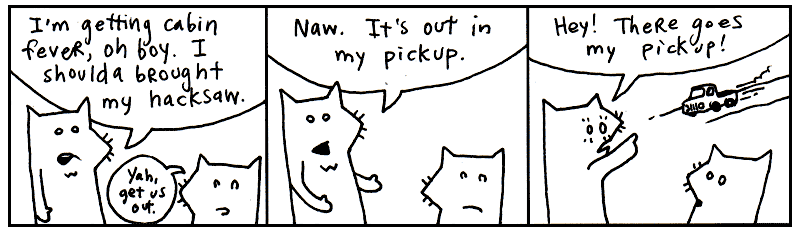
\includegraphics[width=1.0\textwidth]{cache/17.png}

{\bf Say aloud each of the parts of speech used below.}


\begin{lstlisting}[basicstyle=\ttfamily\color{basiccolor},
    commentstyle = \ttfamily\color{commentcolor},
    keywordstyle=\ttfamily\color{keywordscolor},
    stringstyle=\color{stringcolor},
    language=Ruby,
    basicstyle=\small\ttfamily,
    showstringspaces=false,
  ]

 require 'net/http' 
 Net::HTTP.start( 'www.ruby-lang.org', 80 ) do |http| 
     print( http.get( '/en/LICENSE.txt' ).body ) 
 end

\end{lstlisting}


The first line is a method call.  The {\em method} called
\lstinline[breaklines=true]|require| is used.  A {\em string} is
passed to the method containing
\lstinline[breaklines=true]|'net/http'|.  Think of this first line of
code as a sentence.  We have told Ruby to load some helper code, the
\lstinline[breaklines=true]|Net::HTTP| library.

	\begin{sidebar}{Seven Moments of Zen from My Life}{100}
		\textit{(cont'd)}
		\begin{enumerate}
			\setcounter{enumi}{4}
			\item 14. Riding my bike out on the pier with my coach who is jogging behind me as the sun goes down right after I knocked out Piston Honda in the original Nintendo version of Mike Tyson's Punch-Out.
			\item 11. Sick. Watching Heathcliff on television. For hours, it was Heathcliff. And he was able to come right up close to my face. His head spun toward me. His face pulsed back and forth, up close, then off millions of miles away. Sound was gone. In fractions of a second, Heathcliff filled the universe, then blipped off to the end of infinity. I heard my mother's voice trying to cut through the cartoon. Heathclose, Heathaway, Heathclose, Heathaway. It was a religious rave with a cat strobe and muffled bass of mother's voice. (I ran a fever of 105 that day.)
			\item 18. Bought myself a gigapet. A duck. Fed it for awhile. Gave it a bath. Forgot about it for almost a couple months. One day, while cleaning, I found a chain and he was there on the end. Hey, little duck. Mad freaky, hoppin' around with his hair out, squawking diagonal lines. In a tuxedo.
		\end{enumerate}
	\end{sidebar}

The next three lines all go together.  The {\em constant}
\lstinline[breaklines=true]|Net::HTTP| refers to the library we loaded
above. We are using the {\em method}
\lstinline[breaklines=true]|start| from the library.  Into the method,
we're sending a {\em string}
\lstinline[breaklines=true]|'www.ruby-lang.org'| and the {\em number}
\lstinline[breaklines=true]|80|.

The word \lstinline[breaklines=true]|do| opens a {\em block}.  The
block has one {\em block variable} \lstinline[breaklines=true]|http|.
Inside the block, the {\em method} \lstinline[breaklines=true]|print|
is called.  What is being printed?

From the {\em variable} \lstinline[breaklines=true]|http|, the {\em
  method} \lstinline[breaklines=true]|get| is called.  Into
\lstinline[breaklines=true]|get|, we pass a {\em string} containing
the path \lstinline[breaklines=true]|'/en/LICENSE.txt'|.  Now, notice
that another method is chained onto \lstinline[breaklines=true]|get|.
The {\em method} \lstinline[breaklines=true]|body|.  Then, the block
closes with \lstinline[breaklines=true]|end|.

Doing okay?  Just out of curiousity, can you guess what this example
does?  Hopefully, you're seeing some patterns in Ruby.  If not, just
shake your head vigorously while you've got these examples in your
mind.  The code should break apart into manageable pieces.

For example, this pattern is used a number of times:

\begin{quote}
{\em variable} . {\em method} ( {\em method arguments} )\end{quote}


You see it inside the block:

\begin{quote}
\lstinline[breaklines=true]|http.get( '/en/LICENSE.txt' )|\end{quote}


We're using Ruby to get a web page.  You've probably used HTTP with
your web browser.  HTTP is the Hypertext Transfer Protocol.  HTTP is
used to transfer web pages across the internet.  Conceptualize a bus
driver that can drive across the internet and bring back web pages for
us.  On his hat are stitched the letters HTTP.

The variable \lstinline[breaklines=true]|http| is that bus driver.
The {\em method} is a message to the bus driver.  Go
\lstinline[breaklines=true]|get| the web page called
\lstinline[breaklines=true]|/en/LICENSE.txt|.

So where you see the chain of methods:

\begin{quote}
\lstinline[breaklines=true]|http.get( '/en/LICENSE.txt' ).body|\end{quote}


Since we'll be getting back a web page from the
\lstinline[breaklines=true]|http| bus driver, you can read this in
your brain as:

\begin{quote}
{\em web page} .body\end{quote}


And this bit of code:

\begin{quote}
\lstinline[breaklines=true]|print( http.get( '/en/LICENSE.txt' ).body )|\end{quote}


This code gets the web page.  We send a
\lstinline[breaklines=true]|body| message to the web page, which gives
us all the HTML in a {\em string}.  We then
\lstinline[breaklines=true]|print| that string.  See how the basic
dot-method pattern happens in a chain.  The next chapter will explore
all these sorts of patterns in Ruby.  It'll be good fun.

So, what does this code do?  It prints the HTML for the Ruby home page
to the screen.  Using an web-enabled bus driver.


\section{And So, The Quick Trip Came To An Eased, Cushioned Halt}


	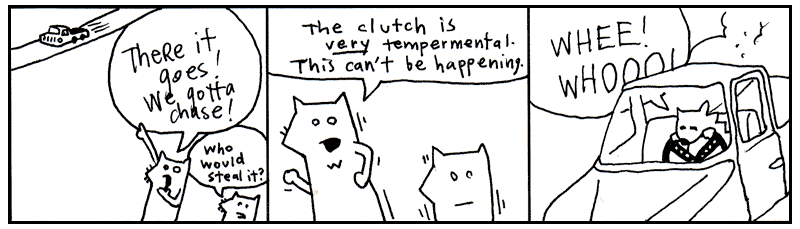
\includegraphics[width=1.0\textwidth]{cache/18.png}

So now we have a problem.  I get the feeling that you are enjoying
this way too much. And you haven't even hit the chapter where I use
jump-roping songs to help you learn how to parse XML!

If you're already enjoying this, then things are really going bad.
Two chapters from now you'll be writing your own Ruby programs.  In
fact, it's right about there that I'll have you start writing your own
role-playing game, your own file-sharing network (a la BitTorrent), as
well as a program that will pull genuine random numbers from the
Internet.

	\parpic[r]{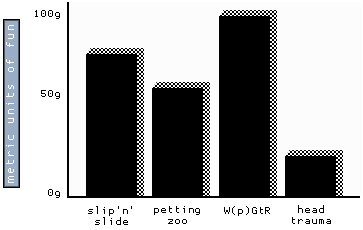
\includegraphics[width=0.45375\textwidth]{cache/19.png}}

And you know (you've got to know!) that this is going to turn into an
obsession.  First, you'll completely forget to take the dog out.
It'll be standing by the screen door, darting its head about, as your
eyes devour the code, as your fingers slip messages to the computer.

Thanks to your neglect, things will start to break.  Your mounds of
printed sheets of code will cover up your air vents.  Your furnace
will choke.  The trash will pile-up: take-out boxes you hurriedly
ordered in, junk mail you couldn't care to dispose of.  Your own
uncleanliness will pollute the air.  Moss will infest the rafters, the
water will clog, animals will let themselves in, trees will come up
through the foundations.

But your computer will be well-cared for.  And you, Smotchkkiss, will
have nourished it with your knowledge. In the eons you will have spent
with your machine, you will have become part-CPU.  And it will have
become part-flesh.  Your arms will flow directly into its ports.  Your
eyes will accept the video directly from DVI-24 pin.  Your lungs will
sit just above the processor, cooling it.

And just as the room is ready to force itself shut upon you, just as
all the overgrowth swallows you and your machine, you will finish your
script.  You and the machine together will run this latest Ruby
script, the product of your obsession.  And the script will fire up
chainsaws to trim the trees, hearths to warm and regulate the house.
Builder nanites will rush from your script, reconstructing your
quarters, retiling, renovating, chroming, polishing, disinfecting.
Mighty androids will force your crumbling house into firm, rigid
architecture.  Great pillars will rise, statues chiseled.  You will
have dominion over this palatial estate and over the encompassing
mountains and islands of your stronghold.

So I guess you're going to be okay.  Whatdya say?  Let's get moving on
this script of yours?
\newpage
\thispagestyle{empty}
\mbox{}
\newpage
\thispagestyle{empty}
\mbox{}
\cleartooddpage

\chapter{Floating Little Leaves of Code}
\vfill
\begin{center}
  
\includegraphics{cache/chapterpoignantguide4.png}
\end{center}
\vspace{2cm}
\newpage
\thispagestyle{empty}
\mbox{}
\clearpage
	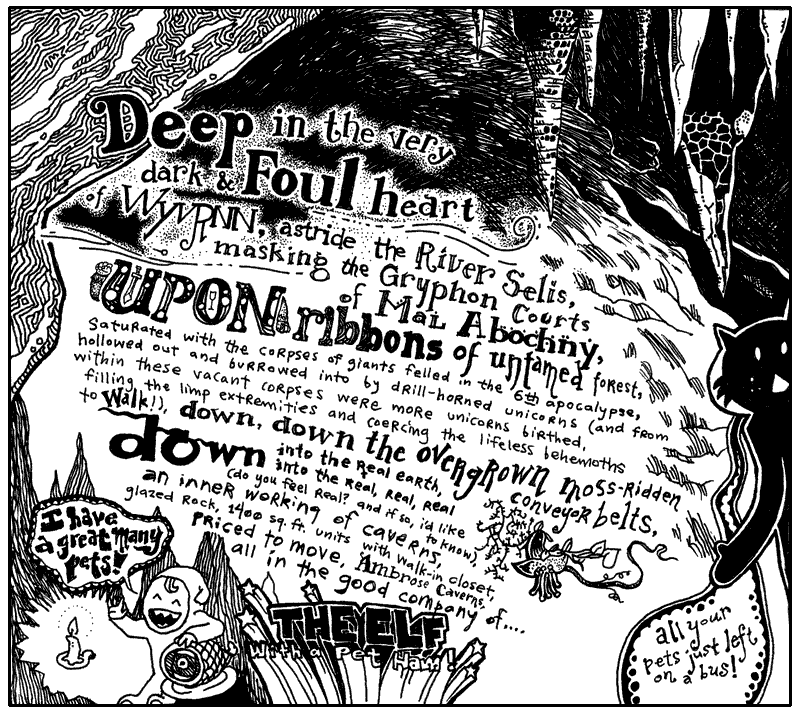
\includegraphics[width=1.0\textwidth]{cache/20.png}
        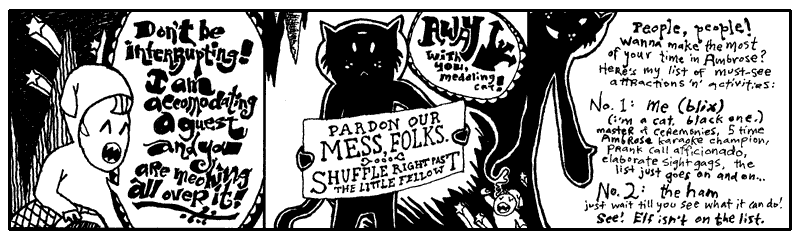
\includegraphics[width=1.0\textwidth]{cache/21.png}
\clearpage
I've never seen the ham do anything but leak juice.  Today, our
business in Ambrose Caverns is with the elf.  He is a crucial part of
the next lessons. Let's all make him feel welcome. Go start warming up
your listening hats!  (And please change out of those ridiculous
stirrup pants.)

A prompt warning: this lesson is much slower.  Stay with it.  This
will be a long, deep breath. The most crucial stage of your
instruction.  It may seem like you're not learning much code at first.
You will be learning concepts.  By the end of this chapter, you will
know Ruby's beauty.  The coziness of the code will become a down
sleeping bag for your own solace.


\section{The Leaf as a Status Symbol in Ambrose}


Alright, Elf.  Give us a quick rundown of the currency issues you've
faced there in your kingdom.

	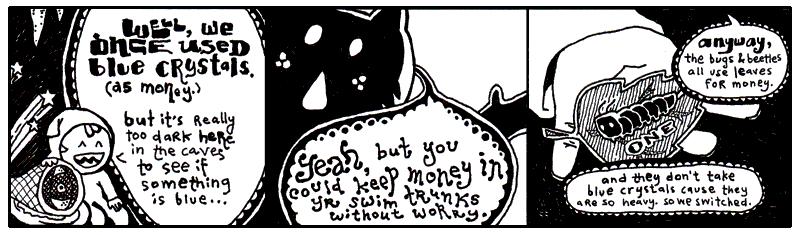
\includegraphics[width=1.0\textwidth]{cache/22.png}

Yeah, that's not the way I remember it.  This Elf was paging me
constantly.  When I refused to call him back, he somehow left a
message on my pager.  Meaning: it beeped a couple times and then
printed out a small slip of paper.  The slip said something to the
effect of, ``Get down here quick!'' and also, ``We've got to rid the
earth of this scourge of enterpreneurial caterpillars, these twisted
insect vikings are suffocating my blue crystals!''

Lately, the exchange rate has settled down between leaves and
crystals.  One treegrown note is worth five crystals.  So the basic
money situation looks like this:


\begin{lstlisting}[basicstyle=\ttfamily\color{basiccolor},
    commentstyle = \ttfamily\color{commentcolor},
    keywordstyle=\ttfamily\color{keywordscolor},
    stringstyle=\color{stringcolor},
    language=Ruby,
    basicstyle=\small\ttfamily,
    showstringspaces=false,
  ]

 blue_crystal = 1 
 leaf_tender = 5

\end{lstlisting}


This example is, like, {\em totally} last chapter.  Still.  It's a
start.  We're setting two {\em variables}. The {\bf equals sign} is
used for {\em assignment}.

Now \lstinline[breaklines=true]|leaf_tender| represents the number
\lstinline[breaklines=true]|5| (as in: five blue crystals.)  This
concept right here is {\bf half of Ruby}.  We're {\em defining}.
We're {\em creating}.  This is half of the work.  Assignment is the
most basic form of defining.

You can't complain though, can you Elf?  You've built an empire from
cashing your blue crystals into the new free market among the forest
creatures.  (And even though he's an elf to us, he's a tall monster to
them.)

	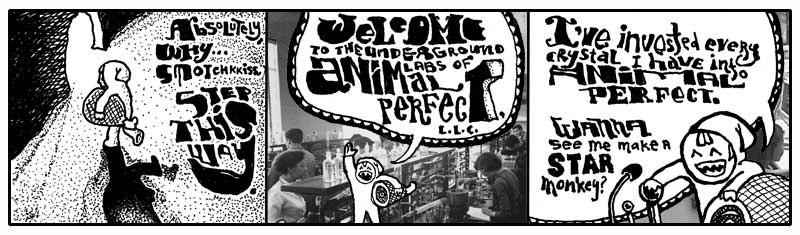
\includegraphics[width=1.0\textwidth]{cache/23.png} Nonono.
        Hang on a sec.  You're not ready for what the Elf here is
        doing in his caves. You'll think it's all positively inhumane,
        naughty, sick, tweeested, yada yada.



\subsection{ Now You're Going to Hear the Animal Perfect Mission
  Statement Because This Is A Book And We Have Time And No Rush,
  Right?}



Back, back, way back before speedboats, I owned a prize race horse who
took a stumble on the track.  She did ten front flips and crashed into
a guy who was carrying a full jar of mayonnaisse.  We had blood and
mayonnaisse up and down the track.  Needless to say, she was a
disaster.

The vet took one look at her and swore she'd never walk again.  Her
legs were gone and the vet wouldn't allow a legless horse to just sit
around.  We'd need to put her down.  He swore his life and career on
it, insisting we divide into two parallel lines.  The people who could
not refute the doctor's claims on one side; those too stubborn to
accept his infallable medical reasoning on the other.  The Elf, his
pet ham, and I were the only ones in that second line.

	\begin{sidebar}{The Scarf Eaters}{100}
		I hate to intrude upon your instruction, but I've already walked all over it enough to warrant some further disregard. Can I go over my next project with you?\vspace{6px}
		
I've pledged to write another book. \textit{(Trombones.)} The good news is that I won't actually be writing any of it. You won't have to endure any more of this inane blathering.\vspace{6px}

It's over between me and words. I'd love to stick around and exploit them each, one after another, but it's all becoming quite predictable, wouldn't you say? Eventually, they will all be used and I'd have to come up with fake words and that would be way too cnoofy.\vspace{6px}

	Now. The deal isn't cut yet, but I'm in negotiations with Anna Quindlen to do my ghost writing. We're tag-teaming on a book that's going to blow the (Poignant) Guide right out of your hands. To put it bluntly, the Guide will be worthless. You won't be able to pile enough pomegranates on top of the thing.\vspace{6px}
	
So this new book. The Scarf Eaters. It's a coming-of-age novel. But it's also a beginner's guide to Macromedia Flash. It's like Judy Blume crossed Praystation. It's like 0sil8 starring Hillary Duff.\vspace{6px}

I don't want to give away the plot at all, but to tug your appetite I'll just say this: one kid talks to his dead brother in ActionScript. More to come.
	\end{sidebar}

So while the others heaped up trophies and great wreaths around the
horse, bidding it a fond farewell before the bullet came to take him
home, the Elf and I frantically pawed the Internet for answers.  We
took matter into our own hands, cauterizing her leg wounds with live
crawdads.  It worked great!  We now had a horse again.  Or at least: a
horse body with a crustaceous abdominal frosting.

She scurried everywhere after that and lived for years in pleasantly
moist underground cavities.

Animal Perfect is now the future of animal enhancement.  They build
new animals and salvage old-style animals for parts.  Of course,
they've come a long ways. When Animal Perfect started, you'd see a
full-grown bear walk into Animal Perfect and you'd see a full-grown
bear with sunglasses walk out.  Completely cheesy.

Stick around and you'll see a crab with {\em his own jet pack}.
That's a new 2004 model jetcrab.

But now, the whole operation is up and running.  And the cleanliness
of the place is astonishing. All the equipment is so shiny.
Everything is in chrome.  Oh, and all the staff have concealed
weapons.  They're trained to kill anyone who enters unannounced.  Or,
if they run out of bullets, they're trained to pistol whip anyone who
enters unannounced.

Elf, make me a starmonkey.

	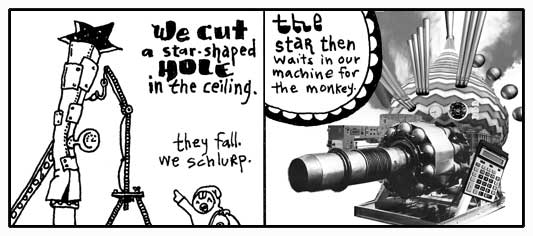
\includegraphics[width=0.66625\textwidth]{cache/24.png}

Some imaginary Ruby for you:

\begin{quote}
\lstinline[breaklines=true]|pipe.catch_a_star|\end{quote}


Variable \lstinline[breaklines=true]|pipe|.  Method
\lstinline[breaklines=true]|catch_a_star|.  A lot of Rubyists like to
think of methods as a message. Whatever comes before the dot is handed
the message.  The above code tells the
\lstinline[breaklines=true]|pipe| to
\lstinline[breaklines=true]|catch_a_star|.

This is the {\bf second half} of Ruby.  Putting things in motion.
These things you define and create in the first half start to {\em
  act} in the second half.

\begin{enumerate}
\item Defining things.
\item Putting those things into action.
\end{enumerate}

So what if the star catching code works?  Where does the star go?

\begin{quote}
\lstinline[breaklines=true]|captive_star = pipe.catch_a_star|\end{quote}


See, it's up to you to collect the miserable, little star.  If you
don't, it'll simply vanish. Whenever you use a method, you'll always
be given something back.  You can ignore it or use it.

{\em If you can learn to use the answers that methods give you back,
  then you will {\bf dominate}.}

	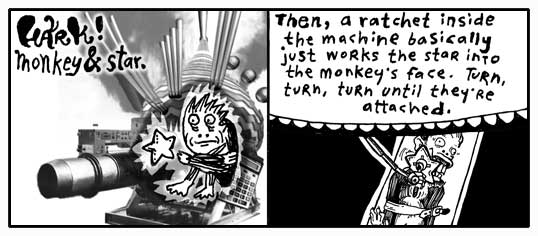
\includegraphics[width=0.6725\textwidth]{cache/25.png}

Quickly then.

\begin{quote}
\lstinline[breaklines=true]|starmonkey = ratchet.attach( captive_monkey, captive_star )|\end{quote}


The \lstinline[breaklines=true]|ratchet| gets an
\lstinline[breaklines=true]|attach| message.  What needs to be
attached?  The {\em method arguments}: the
\lstinline[breaklines=true]|captive_monkey| and the
\lstinline[breaklines=true]|captive_star|.  We are given back a
\lstinline[breaklines=true]|starmonkey|, which we have decided to hang
on to.

	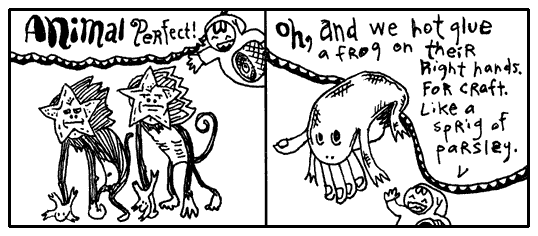
\includegraphics[width=0.6725\textwidth]{cache/26.png}

This is turning out to be such a short, little proggie that I'm just
going to put it all together as one statement.

\begin{quote}
\lstinline[breaklines=true]|starmonkey = ratchet.attach( captive_monkey, pipe.catch_a_star ) + deco_hand_frog|\end{quote}


See how \lstinline[breaklines=true]|pipe.catch_a_star| is right in the
arguments for the method?  The caught star will get passed right to
the ratchet.  No need to find a place to put it.  Just let it go.


\section{Small and Nearly Worthless}


	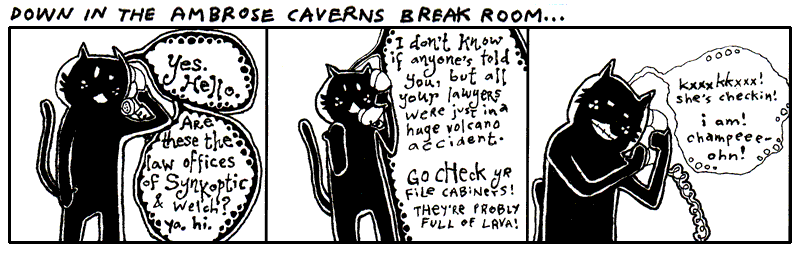
\includegraphics[width=1.0\textwidth]{cache/27.png}

The hotel here in Ambrose is no good at all.  The beds are all
lumpy. The elevator is tiny.  One guy put all his bags in the elevator
and found out there wasn't room for him.  He hit the button and chased
up the stairs after it all.  But the stairwell turned out to be too
narrow and his shoulders got wedged going up.

The soap mini-bars they give you are sized down for elves, so it's
impossible to work up a lather.  I hate it.  I keep mistaking them for
contact lenses.

I turned on the faucet and nothing came out.  Thing is: Ambrose is a
place with magical properties, so I took a chance.  I put my hands
under the spigot.  Invisible, warm wetness.  I felt the hurried
sensation of running water, darting through my fingers.  When I took
my hands away, they were dry and clean.

It was an amazing nothingness to experience.  It was just like
\lstinline[breaklines=true]|nil|.



\subsection{Nil}



In Ruby, \lstinline[breaklines=true]|nil| represents an emptiness.  It
is {\bf without value}.  It isn't zero. Zero is a number.

It's Ruby's own walking dead, a flatlined keyword.  You can't add to
it, it doesn't evolve.  But it's terribly popular.  This skeleton's
smiling in all the pictures.

\begin{quote}
\lstinline[breaklines=true]|plastic_cup = nil|\end{quote}


The above \lstinline[breaklines=true]|plastic_cup| is {\bf empty}.
You could argue that the \lstinline[breaklines=true]|plastic_cup|
contains something, a \lstinline[breaklines=true]|nil|.  The
\lstinline[breaklines=true]|nil| represents the emptiness, though, so
go ahead and call it empty.

Some of you who have programmed before will be tempted to say the
\lstinline[breaklines=true]|plastic_cup| is {\bf undefined}.  How
about let's not.  When you say a variable is undefined, you're saying
that Ruby simply has no recollection of the variable, it doesn't know
the var, it's absolutely non-existent.

But Ruby is aware of the \lstinline[breaklines=true]|plastic_cup|.
Ruby can easily look in the
\lstinline[breaklines=true]|plastic_cup|. It's {\bf empty}, but not
          {\bf undefined}.

\newpage



\subsection{False}



	\parpic[l]{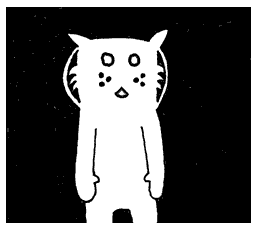
\includegraphics[width=0.3225\textwidth]{cache/28.png}}

{\em The cat Trady Blix.  Frozen in emptiness.  Immaculate whiskers
  rigid.  Placid eyes of lake.  Tail of warm icicle.  Sponsored by a
  Very Powerful Pause Button.}

The darkness surrounding Blix can be called {\bf negative space}.
Hang on to that phrase. Let it suggest that the emptiness has a
negative connotation.  In a similar way,
\lstinline[breaklines=true]|nil| has a slightly sour note that it
whistles.

Generally speaking, {\bf everything in Ruby has a positive charge to
  it}.  This spark flows through strings, numbers, regexps, all of it.
Only two keywords wear a shady cloak: \lstinline[breaklines=true]|nil|
and \lstinline[breaklines=true]|false| draggin us down.

You can {\bf test that charge} with an \lstinline[breaklines=true]|if|
keyword.  It looks very much like the \lstinline[breaklines=true]|do|
blocks we saw in the last chapter, in that both end with an
\lstinline[breaklines=true]|end|.


\begin{lstlisting}[basicstyle=\ttfamily\color{basiccolor},
    commentstyle = \ttfamily\color{commentcolor},
    keywordstyle=\ttfamily\color{keywordscolor},
    stringstyle=\color{stringcolor},
    language=Ruby,
    basicstyle=\small\ttfamily,
    showstringspaces=false,
  ]

 if plastic_cup 
   print "Plastic cup is on the up 'n' up!" 
 end

\end{lstlisting}


If \lstinline[breaklines=true]|plastic_cup| contains either
\lstinline[breaklines=true]|nil| or
\lstinline[breaklines=true]|false|, you won't see anything print to
the screen.  They're not on the \lstinline[breaklines=true]|if| guest
list.  So \lstinline[breaklines=true]|if| isn't going to run any of
the code it's protecting.

But \lstinline[breaklines=true]|nil| and
\lstinline[breaklines=true]|false| need not walk away in shame.  They
may be of questionable character, but
\lstinline[breaklines=true]|unless| runs a smaller establishment that
caters to the bedraggled. The \lstinline[breaklines=true]|unless|
keyword has a policy of {\bf only allowing those with a negative
  charge in}. Who are: \lstinline[breaklines=true]|nil| and
\lstinline[breaklines=true]|false|.


\begin{lstlisting}[basicstyle=\ttfamily\color{basiccolor},
    commentstyle = \ttfamily\color{commentcolor},
    keywordstyle=\ttfamily\color{keywordscolor},
    stringstyle=\color{stringcolor},
    language=Ruby,
    basicstyle=\small\ttfamily,
    showstringspaces=false,
  ]

 unless plastic_cup 
   print "Plastic cup is on the down low."  
 end

\end{lstlisting}


You can also use \lstinline[breaklines=true]|if| and
\lstinline[breaklines=true]|unless| at the {\bf end of a single line
  of code}, if that's all that is being protected.


\begin{lstlisting}[basicstyle=\ttfamily\color{basiccolor},
    commentstyle = \ttfamily\color{commentcolor},
    keywordstyle=\ttfamily\color{keywordscolor},
    stringstyle=\color{stringcolor},
    language=Ruby,
    basicstyle=\small\ttfamily,
    showstringspaces=false,
  ]

 print "Yeah, plastic cup is up again!"  if plastic_cup 
 print "Hardly. It's down." unless plastic_cup

\end{lstlisting}


And another nice trick: stack the \lstinline[breaklines=true]|if| and
\lstinline[breaklines=true]|unless|.


\begin{lstlisting}[basicstyle=\ttfamily\color{basiccolor},
    commentstyle = \ttfamily\color{commentcolor},
    keywordstyle=\ttfamily\color{keywordscolor},
    stringstyle=\color{stringcolor},
    language=Ruby,
    basicstyle=\small\ttfamily,
    showstringspaces=false,
  ]

 print "We're using plastic 'cause we don't have glass." if plastic_cup unless glass_cup

\end{lstlisting}

	\begin{sidebar}{Make Your Own Starmonkey!}{120}
		1. Turn a mug upside-down.
		
		\sidebarImg{cache/sidebar411.jpg}
		
		2. Attach an apple with a rubber band.
		
		\sidebarImg{cache/sidebar412.jpg}
		
		3. Shove car keys into the sides of the apple.
		
		\sidebarImg{cache/sidebar413.jpg}
		
		\textit{(cont'd)} 
	\end{sidebar}

This trick is a gorgeous way of expressing, {\em Do this only if {\bf
    a} is true and {\bf b} isn't true}.

Now that you've met \lstinline[breaklines=true]|false|, I'm sure you
can see what's on next.


\subsection{True}



\begin{quote}
\lstinline[breaklines=true]|approaching_guy = true|\end{quote}


I saw \lstinline[breaklines=true]|true| at the hotel buffet tables
today.  I cannot stand that guy. His stance is way too wide.  And
you've never met anyone who planted his feet so hard in the ground.
He wears this corny necklace made out of shells.  His face exudes this
brash confidence.  (You can tell he's exerting all of his restraint
just to keep from bursting into Neo flight.)

To be honest, I can't be around someone who always has to be
right. This \lstinline[breaklines=true]|true| is always saying,
``A-OK.''  Flashing hang ten.  And seriously, he loves that necklace.
Wears it constantly.

As you'd suspect, he's backstage at everything on the
\lstinline[breaklines=true]|if| event schedule.

\begin{quote}
\lstinline[breaklines=true]|print "Hugo Boss" if true| acts like
\lstinline[breaklines=true]|print "Hugo Boss"|.\end{quote}


Occasionally, \lstinline[breaklines=true]|if| will haul out the
velvet ropes to exercise some crowd control.  The {\bf double equals}
gives the appearance of a short link of ropes, right along the sides
of a red carpet where only \lstinline[breaklines=true]|true| can be
admitted.


\begin{lstlisting}[basicstyle=\ttfamily\color{basiccolor},
    commentstyle = \ttfamily\color{commentcolor},
    keywordstyle=\ttfamily\color{keywordscolor},
    stringstyle=\color{stringcolor},
    language=Ruby,
    basicstyle=\small\ttfamily,
    showstringspaces=false,
  ]

 if approaching_guy == true 
   print "That necklace is classic."  
 end

\end{lstlisting}


The double equals is simply {\bf an ID check}.  Do the gentleman at
both ends of this rope appear to match?

In this way, you control who \lstinline[breaklines=true]|if| lets in.
If you have a hard time getting along with
\lstinline[breaklines=true]|true| as I do, you can heartily welcome
\lstinline[breaklines=true]|false|.


\begin{lstlisting}[basicstyle=\ttfamily\color{basiccolor},
    commentstyle = \ttfamily\color{commentcolor},
    keywordstyle=\ttfamily\color{keywordscolor},
    stringstyle=\color{stringcolor},
    language=Ruby,
    basicstyle=\small\ttfamily,
    showstringspaces=false,
  ]

 if approaching_guy == false 
   print "Get in here, you conniving devil."
 end

\end{lstlisting}


Same goes for \lstinline[breaklines=true]|unless|.  The gateway is
yours.  Take possession of it.



\subsection{Again, I Want You to Dominate}



Now, you want a head trip?  {\bf The double equals sign is a method.}
Can you guess how it works?  Here, check it out with the dot and
parens:

\begin{quote}
\lstinline[breaklines=true]|approaching_guy.==( true )|\end{quote}


Ruby allows the shortcut, though.  You can drop the dot and back away
slowly.

Now, do you remember what you need to do to {\bf dominate} in Ruby?
{\em Use the answers the methods give you.}


\begin{lstlisting}[basicstyle=\ttfamily\color{basiccolor},
    commentstyle = \ttfamily\color{commentcolor},
    keywordstyle=\ttfamily\color{keywordscolor},
    stringstyle=\color{stringcolor},
    language=Ruby,
    basicstyle=\small\ttfamily,
    showstringspaces=false,
  ]

 if nil.==( true )
   print "This will never see realization."  
 end

\end{lstlisting}


In the above, how is the method's answer being used?

	\begin{sidebar}{Make Your Own Starmonkey!}{200}
		\textit{(cont'd)} 
		
		4. Glue star face.
		
		\sidebarImg{cache/sidebar414.jpg}
		
		You have two complementary star faces waiting in your account.
		
		\sidebarImg{cache/sidebar415.jpg}
		
		\begin{center}
			Standard, placid.
		\end{center}
		
		\sidebarImg{cache/sidebar416.jpg}
		
		\begin{center}
			Eating chalk.
		\end{center}
	\end{sidebar}

Let's take the statement \lstinline[breaklines=true]|nil == true|.
This will fail every time.  No match.  When there's no match, the
double equals method answers with \lstinline[breaklines=true]|false|.
A shake of the head. That answer is given to
\lstinline[breaklines=true]|if|, who can't accept a
\lstinline[breaklines=true]|false|.  The
\lstinline[breaklines=true]|print| never sees realization.


\begin{lstlisting}[basicstyle=\ttfamily\color{basiccolor},
    commentstyle = \ttfamily\color{commentcolor},
    keywordstyle=\ttfamily\color{keywordscolor},
    stringstyle=\color{stringcolor},
    language=Ruby,
    basicstyle=\small\ttfamily,
    showstringspaces=false,
  ]

 at_hotel = true 
 email = if at_hotel 
           "why@hotelambrose.com" 
         else
           "why@drnhowardcham.com" 
         end

\end{lstlisting}


Even though \lstinline[breaklines=true]|if| isn't a method,
\lstinline[breaklines=true]|if| does give a return answer.  Look at
the above and wonder over what happens when
\lstinline[breaklines=true]|at_hotel| is
\lstinline[breaklines=true]|true|.

The \lstinline[breaklines=true]|if| will return the answer given by
the code it chooses to run.  In the case of
\lstinline[breaklines=true]|at_hotel| being true, the first string, my
e-mail address at Hotel Ambrose, will be returned.  The
\lstinline[breaklines=true]|else| keyword marks code which will run,
should \lstinline[breaklines=true]|if| fail.  If
\lstinline[breaklines=true]|at_hotel| is false, the
\lstinline[breaklines=true]|if| will answer with my e-mail address at
Dr. N. Howard Cham's office, where I take my apprenticeship.

Should you have several lines of code in an
\lstinline[breaklines=true]|if| or
\lstinline[breaklines=true]|unless|, {\bf only the answer from the
  last full statement will be used}.


\begin{lstlisting}[basicstyle=\ttfamily\color{basiccolor},
    commentstyle = \ttfamily\color{commentcolor},
    keywordstyle=\ttfamily\color{keywordscolor},
    stringstyle=\color{stringcolor},
    language=Ruby,
    basicstyle=\small\ttfamily,
    showstringspaces=false,
  ]

 email = if at_hotel 
           address = "why" 
           address << "@hotelambrose"
           address << ".com"
         end

\end{lstlisting}


Three lines of code inside the \lstinline[breaklines=true]|if|.  The
first line assigns a string with my name in it to a variable. The
second and third lines add the rest of my e-mail address on to the
end.  The {\bf double less-than \lstinline[breaklines=true]|<<| is the
  concatenation operator}.  To concatenate is to {\bf append}, or {\bf
  add to the end}.

Just as we saw with the equality checker
\lstinline[breaklines=true]|==|, the concatenator is a method.  After
adding to the end of the string, the concatenator also {\bf answers
  with that very string}.  So, the third line, which could be read as
\lstinline[breaklines=true]|address.<<( ".com" )|, gives back
\lstinline[breaklines=true]|address|, which the
\lstinline[breaklines=true]|if| then hands back for
\lstinline[breaklines=true]|email|'s assignment.

Here's a question: what if the \lstinline[breaklines=true]|if| fails?
What if \lstinline[breaklines=true]|at_hotel| is false in the above
example? Is anything returned?  Nothing is assigned to
\lstinline[breaklines=true]|email|, right?

Yes, nothing is returned.  By which I mean:
\lstinline[breaklines=true]|nil| is returned.  And often
\lstinline[breaklines=true]|nil| is a very useful answer.


\begin{lstlisting}[basicstyle=\ttfamily\color{basiccolor},
    commentstyle = \ttfamily\color{commentcolor},
    keywordstyle=\ttfamily\color{keywordscolor},
    stringstyle=\color{stringcolor},
    language=Ruby,
    basicstyle=\small\ttfamily,
    showstringspaces=false,
  ]

 print( if at_hotel.nil?
          "No clue if he's in the hotel."
        elsif at_hotel == true
          "Definitely in."
        elsif at_hotel == false
          "He's out."
        else
          "The system is on the freee-itz."
        end )

\end{lstlisting}


You can use the \lstinline[breaklines=true]|nil?| method on any value
in Ruby.  Again, think of it as a message. To the value: ``Are you
nil?  Are you empty?''

If \lstinline[breaklines=true]|at_hotel| is empty, Ruby doesn't have
any idea if I'm in the hotel or not.  So
\lstinline[breaklines=true]|if| answers with the ``No clue'' string.
In order to handle the \lstinline[breaklines=true]|true| or
\lstinline[breaklines=true]|false| possibilities, the
\lstinline[breaklines=true]|elsif| keyword is used.  While you can
have only one \lstinline[breaklines=true]|if| and one
\lstinline[breaklines=true]|else|, you can fill the inbetween with an
exorbitant number of \lstinline[breaklines=true]|elsif| keywords.
Each \lstinline[breaklines=true]|elsif| acts as {\bf a further
  \lstinline[breaklines=true]|if| test}.  Checking for a positive
charge.

If you're doing okay at this point, then you're in tip-top shape for
the rest of the book.  You have seen some pretty tough code in the
last few examples.  You strong fellow.


\section{Chaining Delusions Together}


	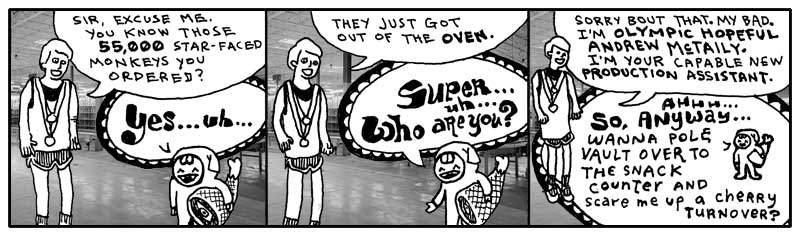
\includegraphics[width=1.0\textwidth]{cache/29.png}

You finish reading the above comic and retire to your daybed for
reflection. It's one of those canopy affairs which is always logjammed
with pillows.  You sit atop the pile, gazing out upon the world.  You
see the tall smokestacks belching wide spools of fume and haze.  The
tangled concourses of freeways smattered with swift, shimmering
traffic is but a gently pulsing eye muscle from your vantage point.

It is all so fantastic.  How the colors of the horizon spread across
the landscape as a great mix of butter and grease with a tablespoon of
vanilla extract.

Yet, for all of the beauty which beckons for your attention, the
images of the Elf and his Olympic Hopeful return.  And more
especially, that order for {\bf 55,000} starmonkeys.  {\em 55,000
  starmonkeys}, you think.  {\em Fifty-five Thousand}.

You think of just the number itself.  {\em 55,000}.  It's walking down
a road.  It might be in a forest, you don't know for sure as your eyes
are fixed right on the number itself.  It's stopping and talking to
people.  To tennis players, to a men's choral group.  There is
merriment and good feeling.  When it laughs, its lower zeros quiver
with glee.

You want to talk to it.  You want to skip along that forest trail with
it.  You want to climb aboard a jet bound to Brazil with it.  And
after five days and four nights at the leisureful Costa do Sauipe
Marriott Resort \& Spa, to marry it, to bear a family of 55,000
starmonkeys with it. To take possession of Nigeria with it.

With a flying leap, you dismount your pillow tower of isolation.
Scrambling with the key, you unlock your roll top desk and pull out a
sheet of paper, holding it firmly upon the desk.  You begin
scribbling.

\begin{quote}


 {\em Take possession of Nigeria with my new 55,000 starmonkeys}...

 

 {\em Over it, build Nigeria-sized {\bf vegetarians only} casino and
   go-cart arena}...

 

 {\em Wings... we could have our own special sauce on the wings that's
   different}...

 

 {\em Mustard + codeine = Smotchkkiss' Starry Starmonkey Glow
   Sauce}...

 

 {\em Franchise, franchise... logos}...

 

 {\em Employee instructional videos}...

 

 {\em When you give the customer change, let them reach inside the
   frog on your hand to get it}...

 

 {\em If they have no change, at least put their receipt some place
   where they have to touch the frog}...

 

 {\em We're leveling the playing field here}...

 

 {\em Advertise cheap pizza, let's make our money off soda}...

 

 {\em Collect all 4 frosted glasses}...

\end{quote}


Wow, the ideas are really coming out.  You literally had to smack
yourself to stop.  We need to put these in a safe place.  Actually, we
should store them on your computer and mangle the words.  You look out
the window and watch for FBI.  I'm going to start this script.



\subsection{The Flipping Script}

\begin{lstlisting}[basicstyle=\ttfamily\color{basiccolor},
    commentstyle = \ttfamily\color{commentcolor},
    keywordstyle=\ttfamily\color{keywordscolor},
    stringstyle=\color{stringcolor},
    language=Ruby,
    basicstyle=\small\ttfamily,
    showstringspaces=false,
  ]

 print "Type and be diabolical: " 
 idea_backwards = gets.reverse

\end{lstlisting}


Let this script be your confidante.  It will ask for evil plans and
turn their letters backwards. The \lstinline[breaklines=true]|gets|
method is {\bf built into Ruby}.  It's a {\bf kernel method} like
\lstinline[breaklines=true]|print|.  This method
\lstinline[breaklines=true]|gets| will pause Ruby to let you type.
When you hit {\em Enter}, \lstinline[breaklines=true]|gets| will then
stop paying attention to your keyboard punchings and answer back to
Ruby with a string that contains everything you typed.  The
\lstinline[breaklines=true]|reverse| method is then used on the string
that \lstinline[breaklines=true]|gets| is giving back.  The
\lstinline[breaklines=true]|reverse| method is part of the
\lstinline[breaklines=true]|String| class.  Which means that {\bf
  anything which is a string has the
  \lstinline[breaklines=true]|reverse| method available}.  More on
classes in the next chapter, for now just know that {\bf a lot of
  methods are only available with certain types of values}.

I don't think \lstinline[breaklines=true]|reverse| is going to cut it.
The authorities only need to put a mirror to ``airegiN fo noissessop
ekaT.''  Bust us when starmonkeys start to touch down in Lagos.

The capital letters give it away.  Maybe if we uppercase all letters
in the string before we reverse it.


\begin{lstlisting}[basicstyle=\ttfamily\color{basiccolor},
    commentstyle = \ttfamily\color{commentcolor},
    keywordstyle=\ttfamily\color{keywordscolor},
    stringstyle=\color{stringcolor},
    language=Ruby,
    basicstyle=\small\ttfamily,
    showstringspaces=false,
  ]

 idea_backwards = gets.upcase.reverse

\end{lstlisting}




\subsection{Your Repetitiveness Pays Off}



You hand me a legal pad, doused in illegible shorthand.  Scanning over
it, I start to notice patterns.  That you seem to use the same set of
words repeatedly in your musings.  Words like {\em starmonkey}, {\em
  Nigeria}, {\em firebomb}.  Some phrases even.  {\em Put the kabosh
  on.} That gets said a lot.

Let us disguise these foul terms, my brother.  Let us obscure them
from itching eyes that cry to know our delicate schemes and to thwart
us from having great pleasure and many go-carts. We will replace them
with the most innocent language.  New words with secret meaning.

I start up a word list, a Ruby \lstinline[breaklines=true]|Hash|,
which contains these oft seen and dangerous words of yours. In the
Hash, each dangerous word is matched up against a code word (or
phrase).  The code word will be swapped in for the real word.


\begin{lstlisting}[basicstyle=\ttfamily\color{basiccolor},
    commentstyle = \ttfamily\color{commentcolor},
    keywordstyle=\ttfamily\color{keywordscolor},
    stringstyle=\color{stringcolor},
    language=Ruby,
    basicstyle=\small\ttfamily,
    showstringspaces=false,
  ]

 code_words = {
   'starmonkeys' => 'Phil and Pete, those prickly chancellors of the New Reich',
   'catapult' => 'chucky go-go', 'firebomb' => 'Heat-Assisted Living',
   'Nigeria' => "Ny and Jerry's Dry Cleaning (with Donuts)",
   'Put the kabosh on' => 'Put the cable box on'
 }

\end{lstlisting}

The words which are placed before the arrow are called {\bf keys}.
The words after the arrows, the definitions, are often just called
{\bf values}.

Notice the double quotes around \lstinline[breaklines=true]|Ny and Jerry's Dry Cleaning (with Donuts)|.  
Since a single quote is being used an apostrophe, we can't use single
quotes around the string.  (Although, you can use single quotes if you
put a backslash before the apostrophe such as:
\lstinline[breaklines=true]|'Ny and Jerry\'s Dry Cleaning (with Donuts)'|.)

Should you need to look up a specific word, you can do so by using the
{\bf square brackets} method.

\begin{quote}
\lstinline[breaklines=true]|code_words['catapult']| will answer with
the string \lstinline[breaklines=true]|'chucky go-go'|.\end{quote}


Look at the square brackets as if they are a wooden pallet the word is
sitting upon. A forklift could slide its prongs into each side of the
pallet and bring it down from a shelf back in the warehouse.  The word
on the pallet is called the {\em index}. We are asking the forklift to
find the index for us and bring back its corresponding value.

If you've never been to a warehouse, you could also look at the
brackets as handles. Imagine an industrious worker putting on his work
gloves and hefting the index back to your custody.  If you've never
used handles before, then I'm giving you about thirty seconds to find
a handle and use it before I blow my lid.

As with many of the other operators you've seen recently, the index
brackets are simply a shortcut for a method.

\begin{quote}
\lstinline[breaklines=true]|code_words.[]( 'catapult' )| will answer
with the string \lstinline[breaklines=true]|'chucky go-go'|.\end{quote}




\subsection{Making the Swap}



I went ahead and saved the Hash of code words to a file called {\bf
  wordlist.rb}.


\begin{lstlisting}[basicstyle=\ttfamily\color{basiccolor},
    commentstyle = \ttfamily\color{commentcolor},
    keywordstyle=\ttfamily\color{keywordscolor},
    stringstyle=\color{stringcolor},
    language=Ruby,
    basicstyle=\small\ttfamily,
    showstringspaces=false,
  ]

 require 'wordlist'

 # Get evil idea and swap in code words
 print "Enter your new idea: "
 idea = gets
 code_words.each do |real, code|
   idea.gsub!( real, code )
 end

 # Save the jibberish to a new file
 print "File encoded.  Please enter a name for this idea: "
 idea_name = gets.strip
 File::open( "idea-" + idea_name + ".txt", "w" ) do |f|
   f << idea
 end

\end{lstlisting}

Script starts by pulling in our word list.  Like
\lstinline[breaklines=true]|gets| and
\lstinline[breaklines=true]|print|, the
\lstinline[breaklines=true]|require| method is a kernel method, you
can use it anywhere.  I give it the string
\lstinline[breaklines=true]|'wordlist'| and it will look for a file
named {\bf wordlist.rb}.

After that, there are two sections.  I am marking these sections with
comments, the lines that start with {\bf pound} symbols.  Comments are
{\bf useful notes} that accompany your code.  Folks who come wandering
through your code will appreciate the help.  When going through your
own code after some time has passed, comments will help you get back
into your mindset.  And there's software out there that can take your
comments and build documents from them.  (RDoc and Ri -- see Expansion
Pak \#1!)

I like comments because I can skim a big pile of code and spot the
highlights.

As the comments tell us, the first section asks you for your evil idea
and swaps in the new code words.  The second section saves the encoded
idea into a new text file.


\begin{lstlisting}[basicstyle=\ttfamily\color{basiccolor},
    commentstyle = \ttfamily\color{commentcolor},
    keywordstyle=\ttfamily\color{keywordscolor},
    stringstyle=\color{stringcolor},
    language=Ruby,
    basicstyle=\small\ttfamily,
    showstringspaces=false,
  ]

 code_words.each do |real, code|
   idea.gsub!( real, code )
 end

\end{lstlisting}

You see the \lstinline[breaklines=true]|each| method?  The
\lstinline[breaklines=true]|each| method is all over in Ruby.  It's
available for Arrays, Hashes, even Strings.  Here, our
\lstinline[breaklines=true]|code_words| dictionary is kept in a Hash.
This \lstinline[breaklines=true]|each| method will hurry through {\bf
  all the pairs of the Hash}, one dangerous word matched with its code
word, handing each pair to the \lstinline[breaklines=true]|gsub!|
method for the actual replacement.

In Ruby, \lstinline[breaklines=true]|gsub| is short for {\em global
  substitution}.  The method is used to search and replace. Here, we
want to find all the occurences of a dangerous word and replace with
its safe code word.  With \lstinline[breaklines=true]|gsub|, you
provide the {\bf word to find as the first argument}, then the {\bf
  word to put in its place as the second argument}.

Why aren't we hanging on to the answer from
\lstinline[breaklines=true]|gsub|?  Doesn't
\lstinline[breaklines=true]|gsub| give us an answer back that we
should keep?  You'd think the line would read:


\begin{lstlisting}[basicstyle=\ttfamily\color{basiccolor},
    commentstyle = \ttfamily\color{commentcolor},
    keywordstyle=\ttfamily\color{keywordscolor},
    stringstyle=\color{stringcolor},
    language=Ruby,
    basicstyle=\small\ttfamily,
    showstringspaces=false,
  ]

 safe_idea = idea.gsub( real, code )

\end{lstlisting}


Yes, with \lstinline[breaklines=true]|gsub| we'd need to hang on to
its answer.  We're using a variation of
\lstinline[breaklines=true]|gsub| that is totally hyper.  Notice the
{\bf exclamation mark} on the \lstinline[breaklines=true]|gsub!| used
inside the \lstinline[breaklines=true]|each| block.  The exclamation
mark is a sign that \lstinline[breaklines=true]|gsub!| is a bit of a
zealot.  See, \lstinline[breaklines=true]|gsub!| will go ahead and
{\bf replace the words in \lstinline[breaklines=true]|idea| directly}.
When it's done \lstinline[breaklines=true]|idea| will contain the
newly altered string and you won't be able to find the old string.

Call \lstinline[breaklines=true]|gsub!| a {\bf destructive method}.
It makes its changes to the value directly.  Whereas
\lstinline[breaklines=true]|gsub| will leave the value intact,
answering back with a new string which contains the alterations. (Why
must \lstinline[breaklines=true]|gsub!| scream when he descends upon
his prey?  Merciless assailant!)



\subsection{Text Files of a Madman}



Let us now save the encoded idea to a file.


\begin{lstlisting}[basicstyle=\ttfamily\color{basiccolor},
    commentstyle = \ttfamily\color{commentcolor},
    keywordstyle=\ttfamily\color{keywordscolor},
    stringstyle=\color{stringcolor},
    language=Ruby,
    basicstyle=\small\ttfamily,
    showstringspaces=false,
  ]

 # Save the jibberish to a new file
 print "File encoded.  Please enter a name for this idea: "
 idea_name = gets.strip
 File::open( 'idea-' + idea_name + '.txt', 'w' ) do |f|
   f << idea
 end

\end{lstlisting}

This section starts by asking you for a name by which the idea can be
called.  This name is used to build a file name when we save the idea.

The \lstinline[breaklines=true]|strip| method is for strings.  This
method {\bf trims spaces and blank lines} from the {\bf beginning and
  end} of the string.  This will remove the {\em Enter} at the end of
the string you typed. But it'll also handle spaces if you accidentally
left any.

After we have the idea's name, we open a new, blank text file.  The
file name is built by adding strings together.  If you typed in
\lstinline[breaklines=true]|'mustard-plus-codeine'|, then our math
will be: \lstinline[breaklines=true]|'idea-' + 'mustard-plus-codeine' + '.txt'|.  
Ruby presses these into a single string. 
\lstinline[breaklines=true]|'idea-mustard-plus-codeine.txt'|
is the file.

We're using the class method \lstinline[breaklines=true]|File::open|
to create the new file.  Up until now, we've used several kernel
methods to do our work.  We hand the
\lstinline[breaklines=true]|print| method a string and it prints the
string on your screen.  One secret about kernel methods like
\lstinline[breaklines=true]|print|: they are actually {\bf class
  methods}.

\begin{quote}
\lstinline[breaklines=true]|Kernel::print( "55,000 Starmonkey Salute!")|\end{quote}


What does this mean?  Why does it matter?  It means
\lstinline[breaklines=true]|Kernel| is the center of Ruby's
universe. Wherever you are in your script,
\lstinline[breaklines=true]|Kernel| is right beside you.  You don't
even need to spell \lstinline[breaklines=true]|Kernel| out for Ruby.
Ruby knows to check \lstinline[breaklines=true]|Kernel|.

Most methods are more specialized than
\lstinline[breaklines=true]|print| or
\lstinline[breaklines=true]|gets|.  Take the
\lstinline[breaklines=true]|File::open| for example.  The creator of
Ruby, Matz, has given us many different methods which which read,
rename, or delete files.  They are all organized inside the
\lstinline[breaklines=true]|File| class.

\begin{quote}
\lstinline[breaklines=true]|File::read( "idea-mustard-plus-codeine.txt" )|
will answer back with a string containing all of the text from your
idea file.\end{quote}


\begin{quote}
\lstinline[breaklines=true]|File::rename( "old_file.txt", "new_file.txt" )| 
will rename
\lstinline[breaklines=true]|old_file.txt|.\end{quote}


\begin{quote}
\lstinline[breaklines=true]|File::delete( "new_file.txt" )| will nuke
the new file.\end{quote}


These File methods are all {\bf built right into Ruby}.  They are all
just stored in a container called the
\lstinline[breaklines=true]|File| class.  So, while you can safely
call kernel methods without needing to type
\lstinline[breaklines=true]|Kernel|, Ruby doesn't automatically check
the \lstinline[breaklines=true]|File| class. You'll need to give the
full method name.


\begin{lstlisting}[basicstyle=\ttfamily\color{basiccolor},
    commentstyle = \ttfamily\color{commentcolor},
    keywordstyle=\ttfamily\color{keywordscolor},
    stringstyle=\color{stringcolor},
    language=Ruby,
    basicstyle=\small\ttfamily,
    showstringspaces=false,
  ]

 File::open( 'idea-' + idea_name + '.txt', 'w' ) do |f|
   f << idea
 end

\end{lstlisting}

We pass two arguments into \lstinline[breaklines=true]|File::open|.
The first is the {\bf file name to open}.  The second is a string
containing our {\bf file mode}.  We use
\lstinline[breaklines=true]|'w'|, which means to write to a brand-new
file.  (Other options are: \lstinline[breaklines=true]|'r'| to read
from the file or \lstinline[breaklines=true]|'a'| to add to the end of
the file.)

The file is opened for writing and we are handed back the file in
variable \lstinline[breaklines=true]|f|, which can be seen {\bf
  sliding down the chute into our block}.  Inside the block, we write
to the file.  When the block closes with
\lstinline[breaklines=true]|end|, our file is closed as well.

Notice we use the {\bf concatenator} \lstinline[breaklines=true]|<<|
to write to the file.  We can do this because files have a method
called \lstinline[breaklines=true]|<<| just like strings do.



\subsection{Settle Down, Your Ideas Aren't Trapped}



Here, let's get your ideas back to their original verbage, so you can
rumminate over their brilliance.


\begin{lstlisting}[basicstyle=\ttfamily\color{basiccolor},
    commentstyle = \ttfamily\color{commentcolor},
    keywordstyle=\ttfamily\color{keywordscolor},
    stringstyle=\color{stringcolor},
    language=Ruby,
    basicstyle=\small\ttfamily,
    showstringspaces=false,
  ]

 require 'wordlist'

 # Print each idea out with the words fixed
 Dir['idea-*.txt'].each do |file_name|
   idea = File.read( file_name )
   code_words.each do |real, code|
     idea.gsub!( code, real )
   end
   puts idea
 end

\end{lstlisting}

By now, you should be up to snuff with most of this example.  I won't
bore you with all of the mundane details.  See if you can figure out
how it works on your own.

We have an interesting class method here, though.  The
\lstinline[breaklines=true]|Dir::[]| method searches a directory (some
of you may call them ``folders'').  Just as you've seen with Hashes,
the index brackets can be class methods.  (Can you start to see the
shiny, glinting gorgeousness of Ruby?)

So we're using the forklift to get those files in the directory which
match \lstinline[breaklines=true]|'idea-*.txt'|.  The
\lstinline[breaklines=true]|Dir::[]| method will use the asterisk as a
wildcard.  We're basically saying, ``Match anything that starts with
{\em idea-} and ends with {\em .txt}.''  The forklift shuffles off to
the directory and comes back with a list of all matching files.

That {\bf list of files} will come in the form of
\lstinline[breaklines=true]|Array| the Caterpillar, with a
\lstinline[breaklines=true]|String| for each file.  If you are curious
and want to play with with \lstinline[breaklines=true]|Dir::[]|, try
this:

\begin{quote}
\lstinline[breaklines=true]|p Dir['idea-*.txt']| will
print:\end{quote}


\begin{quote}
\lstinline[breaklines=true]|['idea-mustard-plus-codeine.txt']| ({\em
  an Array of file names!})\end{quote}


Yes, the \lstinline[breaklines=true]|p| method works like
\lstinline[breaklines=true]|print|.  But where
\lstinline[breaklines=true]|print| is designed for displaying strings,
\lstinline[breaklines=true]|p| will print {\em anything}.  Check this
out.

\begin{quote}
\lstinline[breaklines=true]|p File::methods| will print:\end{quote}


\begin{quote}
\lstinline[breaklines=true]|["send", "display", "name", "exist?", "split",|
 ... {\em a whole list of method names!}
  \lstinline[breaklines=true]|]|\end{quote}



\section{The Miracle of Blocks}


	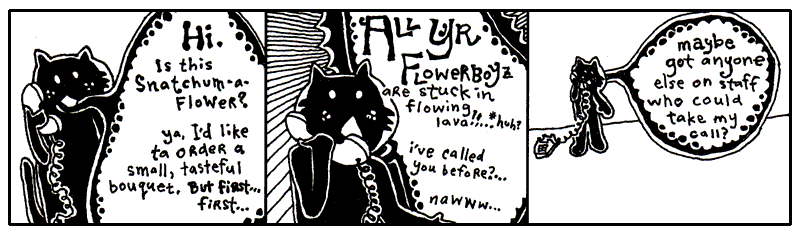
\includegraphics[width=1.0\textwidth]{cache/30.png}

	\begin{sidebar}{Excerpt from The Scarf Eaters}{50}
		\textit{(from Chapter V: A Man in Uniform.)}\vspace{6pt}
		
		In April, the callow lilies came back. They stretched their baby angel wings out and reached for the world. Gently, their tendrils caressed the sullen fence posts until even they lilted lovelier.\vspace{6pt}

		From her bedroom window, Lara watched the lilies exude their staunch femininity. She slipped the tassels of a fresh, carpathian, embroidered scarf into her mouth and ate slowly. The long cloth slid down her throat and tickled as it snaked along her esophagus. She giggled and burped.\vspace{6pt}

		Oh, how the flora drew her in. Looking at flowers went so well with being a teenage girl. She wanted to paint them, so she opened a new Flash template. A blank movie this time. \vspace{6pt}
		
		She set her cursor loose in the garden of her movie's viewable area. Vector white lines below shorter vector yellow lines. She selected the white lines and grouped them together. She even moved them to a new layer entitled ``Cry, Baby Angel, Cry." Then she converted them into a graphic object and moved them to the library.\vspace{6pt}
		
		She felt a warm chill as she moved the long, white petals to her movie's library. It felt so official. I choose you. I name you. Dwell in the comfort of my palace forevermore.\vspace{6pt}

		Heh. She laughed. Colorado Springs was hardly a ``palace." \textit{(cont'd)}
	\end{sidebar}

Since you and I are becoming closer friends as we share this time
together, I should probably let you in on a bit of the history going
on here.  It's a good time for a break I say.

First, you should know that Blix is my cat.  My second pet to
Bigelow. Granted, we hardly see each other anymore.  He's completely
self-sufficient. I'm not exactly sure where he's living these days,
but he no longer lives in the antechamber to my quarters.  He emptied
his savings account about seven months ago.

He does have a set of keys for the house and the Seville.  Should he
ever find himself stranded, I will gladly step away from our
differences and entertain his antics around the house again.

Make no mistake.  I miss having him around.  Can't imagine he misses
my company, but I miss his.



\subsection{A Siren and A Prayer}



I first saw Blix on television when I was a boy.  He had a starring
role on a very gritty police drama called {\em A Siren and A Prayer}.
The show was about a god-fearing police squad that did their jobs, did
them well, and saw their share of miracles out on the beat.  I mean
the officers on this show were {\em great} guys, very religious,
practically clergy.  But, you know, even clergymen don't have the good
sense to kill a guy after he's gone too far. These guys knew where to
draw that line.  They walked that line every day.

	\begin{sidebar}{Excerpt from The Scarf Eaters}{30}
		\textit{(cont'd)} 

		Since they had moved, Dad had only been home once. He had barged through the front door in full uniform and had given quite a start to both Lara and her mother. Her mother had even dropped a head of lettuce -- which head she had just finished washing -- in a pitcher of Lick-M-Aid.\vspace{6pt}
		
		The pitcher was just wide enough for the lettuce and it lodged in there pretty good. Dad came over and yanked at the moist head for sometime until declaring it FUBAR, in a voice both bemused and then crestfallen. He tossed the clotted spout in the trash bin.\vspace{6pt}
		
		It was only later that day that Lara's mother realized that she could have simply halved the lettuce with an electric knife. Dad laughed and slapped his forehead. He then went around and slapped Lara's forehead, and her mother's too, affectionately.
		
		``We just weren't thinking, were we?" is what he said. ``And who dares blame us? We're a real family today. And we shouldn't have to do anything else on the day we got our family back."\vspace{6pt}

		Lara's smiled reflected across the glass of her monitor. She chose the text tool and in 42 point serif typed: ``Dad." She created a path for it and let it tween off the right side of the screen. She cried long after it was gone.
	\end{sidebar}
	
So, it was a pretty bloody show, but they always had a good moral at
the end.  Most times the moral was something along the lines of,
``Wow, we got out of that one quick.''  But there's serious
camaraderie in a statement like that.

The show basically revolved around this one officer.  ``Mad'' Dick
Robinson.  People called him Mad because he was basically insane.  I
can't remember if he was actually clinically insane, but people were
always questioning his decisions.  Mad often blew his top and chewed
out some of the other officers, most of whom had unquestionable moral
character.  But we all know it's a tough world, the stakes are high
out there, and everyone who watched the show held Mad in great regard.
I think everyone on the squad grew quite a bit as people, thanks to
Mad's passion.

The officers couldn't do it all themselves though.  In every single
episode, they plead with a greater force for assistance.  And, in
every single episode, they got their tips from a cat named Terry
(played by my cat Blix.)  He was just a kitten at the time and, as a
young boy tuning into {\em A Siren and A Prayer}, I found myself
longing for my own crime-sniffing cat. Terry took these guys down the
subway tunnels, through the rotting stench of abandoned marinas, into
backdoors of tall, industrial smokestacks.

Sometimes he was all over an episode, darting in and out, preparing
traps and directing traffic. But other times you wouldn't see him the
whole episode.  Then you'd rewind through the whole show and look and
look and look.  You'd give up.  He can't be in that episode.

Still, you can't bear to let it go, so you go comb through the whole
episode with the jog on your remote, combing, pouring over each scene.
And there he is.  Way up behind the floodlight that was turned up too
high.  The one that left Mad with permanent eye damage.  Why?  Why
burn out the retinas of your own colleague, Terry?

But the question never got answered because the series was cancelled.
They started to do special effects with the cat and it all fell apart.
In the last episode of the show, there is a moment where Terry is
trapped at the top of a crane, about to fall into the searing slag in
the furnace of an iron smelt.  He looks back.  No going back.  He
looks down.  Paws over eyes ({\em no joke!}), he leaps from the crane
and, mid-flight, snags a rope and swings to safety, coming down on a
soft antelope hide that one of the workers had presumably been tanning
that afternoon.

People switched off the television set the very moment the scene
aired.  They tried changing the name. First it was {\em God Gave Us a
  Squad}.  {\em Kiss of Pain}.  Then, {\em Kiss of Pain in Maine},
since the entire precinct ended up relocating there.  But the magic
was gone.  I went back to summer school that year to make up some
classes and all the kids had pretty much moved on to football pencils.



\subsection{Blocks}



A couple years ago, I started teaching Blix about Ruby.  When we got
to this part in his lessons, the part that covers blocks, he said to
me, ``Blocks remind me of Mad Dick Robinson.''

``Oh?''  I hadn't heard that name in awhile.  ``I can't see how that
could be.''

``Well, you say blocks can be difficult to understand.''

``They're not difficult,'' I said.  ``A {\bf block} is just {\bf code
  that's grouped together}.''

``And Mad was just an officer, sworn to uphold his duty,'' he said.
``But he was a real miracle to watch out in the field.  Now, this
first example you've shown me...''  He pointed to an example I'd
written down for him.


\begin{lstlisting}[basicstyle=\ttfamily\color{basiccolor},
    commentstyle = \ttfamily\color{commentcolor},
    keywordstyle=\ttfamily\color{keywordscolor},
    stringstyle=\color{stringcolor},
    language=Ruby,
    basicstyle=\small\ttfamily,
    showstringspaces=false,
  ]

 kitty_toys = 
   [:shape => 'sock', :fabric => 'cashmere'] +
   [:shape => 'mouse', :fabric => 'calico'] +
   [:shape => 'eggroll', :fabric => 'chenille'] 
 kitty_toys.sort_by { |toy| toy[:fabric] }

\end{lstlisting}


``This is a small miracle,'' he said. ``I can't deny its beauty.
Look, there are my kitty toys, laid out with their characteristics.
Below them, the block, sorting them by fabric.''

``I apologize if your list of toys looks a bit tricky,'' I said.  Like
you, he had learned about the Array, the caterpillar stapled into the
code, with square brackets on each side and each item separated by
commas.  (Ah, here is one: 
\lstinline[breaklines=true]|['sock', 'mouse', 'eggroll']|.) 
He had also been taught the Hash, which is like a dictionary, with
curly braces on each end which look like small, open books.  Commas in
the Hash between each pair.  Each word in the dictionary matched up
with its definition by an arrow.  (Be beholden:
\lstinline[breaklines=true]|{'blix' => 'cat', 'why' => 'human'}|.)

``Yes, vexing,'' he said.  ``It has square brackets like it's an
Array, but with the arrows like it's a Hash. I don't think you're
going to get away with that.''

``It does seem a bit subversive, doesn't it?''  I said, tease-nudging
him with a spoon.  ``I've done your kitty toy list in a mix of the
two.  I'm using a shortcut.  Which is: {\bf If you use arrows inside
  of an Array, you'll end up with a Hash inside of that Array.}''

``Oh, I see,'' he said.  ``You criss-crossed 'em.  How neat!''

``Yes, yes, you're on it,'' I said.  He was also very good with a
protractor.  ``I have three Arrays, each with a Hash inside.  Notice
the plus signs?  I'm adding them into one big Array.  Here's another
way of writing it...''  I jotted down.


\begin{lstlisting}[basicstyle=\ttfamily\color{basiccolor},
    commentstyle = \ttfamily\color{commentcolor},
    keywordstyle=\ttfamily\color{keywordscolor},
    stringstyle=\color{stringcolor},
    language=Ruby,
    basicstyle=\small\ttfamily,
    showstringspaces=false,
  ]

 kitty_toys = [
   {:shape => 'sock', :fabric => 'cashmere'},
   {:shape => 'mouse', :fabric => 'calico'},
   {:shape => 'eggroll', :fabric => 'chenille'}
 ]

\end{lstlisting}


One Array, which acts as our list of chew toys.  Three Hashes in the
Array to describe each toy.



\subsection{Sorting and Iterating to Save Lives}



``Let's sort your toys by shape now,'' I said.  ``Then, we'll print
them out in that order.''


\begin{lstlisting}[basicstyle=\ttfamily\color{basiccolor},
    commentstyle = \ttfamily\color{commentcolor},
    keywordstyle=\ttfamily\color{keywordscolor},
    stringstyle=\color{stringcolor},
    language=Ruby,
    basicstyle=\small\ttfamily,
    showstringspaces=false,
  ]

 kitty_toys.sort_by { |toy| toy[:shape] }.each do |toy| 
   puts "Blixy has a #{ toy[:shape] } made of #{ toy[:fabric] }"
 end

\end{lstlisting}


``How does \lstinline[breaklines=true]|sort_by| work?'' asked Blix.
``I can tell it's a method you can use with Arrays.  Because
\lstinline[breaklines=true]|kitty_toys| is an Array.  But what is
\lstinline[breaklines=true]|toy|?''

``Okay, \lstinline[breaklines=true]|toy| is a {\bf block argument},''
I said.  ``Remember: the skinny pipes on each side of
\lstinline[breaklines=true]|toy| make it a {\bf chute}.''

``Sure, but it looks like you're using it like a Hash.  Inside the
block you have \lstinline[breaklines=true]|toy[:shape]|. That looks
like a Hash.''

``The \lstinline[breaklines=true]|sort_by| method is an {\bf
  iterator}, Blix.  It {\bf iterates}, or {\bf cycles}, through {\bf a
  list of things}.  You remember that episode when Mad...''

``Episode?'' he said.  Yeah, he can't understand the concept of TV
dramas.  Yeah, I've tried explaining.

``Or, yeah, remember that one {\em eyewitness account} we watched
where Mad was trying to talk down that crazy spelling bee contestant
from the ledge of an college library?''

``I remember it better than you because I was riding in a remote
control plane.''  Yep, it was one of those episodes.

``Do you remember how Mad got the guy to come down?'' I asked.

``People in spelling bees love letters,'' said Blix.  ``So what Mad
did was a genius move on his part. He started with the letter A and
gave reasons, for all the letters of the alphabet, why the guy should
walk back down the building and be safe on the ground.''

```A is for the Architecture of buildings like this,''' I said, in a
gruff Mad voice. ```Which give us hope in a crumbling world.'''

```B is for Big Guys, like your friend Mad the Cop,''' said Blix.
```Guys who help people all the time and don't know how to spell too
great, but still help guys who spell really great.'''

``See, he went through all the letters, one at a time.  He was {\em
  iterating} through them.'' {\em It Err Ate Ing.}

``But the guy jumped anyway, Why.  He jumped off on letter Q or
something.''

```Q is for Quiet Moments that help us calm down and think about all
of life's little pleasures, so we don't get all uptight and starting
goofing around on tiptoes at the very edge of a big, bad building.'''

``And then he jumped,'' said Blix.  He shook his head.  ``You can't
blame Mad.  He did his best.''

``He had a big heart, that's for sure,'' I said, patting Blix on the
shoulder.


\begin{lstlisting}[basicstyle=\ttfamily\color{basiccolor},
    commentstyle = \ttfamily\color{commentcolor},
    keywordstyle=\ttfamily\color{keywordscolor},
    stringstyle=\color{stringcolor},
    language=Ruby,
    basicstyle=\small\ttfamily,
    showstringspaces=false,
  ]

 kitty_toys.sort_by { |toy| toy[:shape] }.each do |toy|
   puts "Blixy has a #{ toy[:shape] } made of #{ toy[:fabric] }"
 end

\end{lstlisting}

``As for your \lstinline[breaklines=true]|sort_by|, it {\bf starts at
  the top} of the list and {\bf goes through each item}, one at a
time. So \lstinline[breaklines=true]|toy| is one of those items.  With
each item, \lstinline[breaklines=true]|sort_by| stops and {\bf slides
  that item down the chute}, under the
\lstinline[breaklines=true]|toy| name, and let's you figure out what
to do with it.''

``Okay, so \lstinline[breaklines=true]|toy| takes turns being each of
the different toys I have.''

``That's right,'' I said.  ``You know how I've really been harping on
{\em using the answers that methods give you}?  Here, we're simply
looking up the toy's shape inside the block.  The block then answers
to \lstinline[breaklines=true]|sort_by| with the shape string, such as
\lstinline[breaklines=true]|"mouse"| or
\lstinline[breaklines=true]|"sock"|.  Once it's done cycling through
the whole list, \lstinline[breaklines=true]|sort_by| will have
alphabetically compared each of the shape strings and will give back a
new sorted Array.''



\subsection{ An Unfinished Lesson}



``That's good enough for today,'' said Blix.  ``Can I have a fresh
saucer of milk, please?''

I filled his saucer to the brim and he guzzled from it for some time
while I took a poker and jabbed at coals in the fireplace.  My mind
wandered and I couldn't help but think further of blocks.  I wondered
what I would teach Blix next.

I probably would have taught him about
\lstinline[breaklines=true]|next|.  When you are iterating through a
list, you may use \lstinline[breaklines=true]|next| to {\bf skip on to
  the next item}.  Here we're counting toys that have a non-eggroll
shape by skipping those that do with
\lstinline[breaklines=true]|next|.


\begin{lstlisting}[basicstyle=\ttfamily\color{basiccolor},
    commentstyle = \ttfamily\color{commentcolor},
    keywordstyle=\ttfamily\color{keywordscolor},
    stringstyle=\color{stringcolor},
    language=Ruby,
    basicstyle=\small\ttfamily,
    showstringspaces=false,
  ]

 non_eggroll = 0
 kitty_toys.each do |toy|
   next if toy[:shape] == 'eggroll'
   non_eggroll = non_eggroll + 1
 end

\end{lstlisting}

I could also have taught him about \lstinline[breaklines=true]|break|,
which {\bf kicks you out of an iterating loop}. In the code below,
we'll print out (with \lstinline[breaklines=true]|p|) each of the toy
Hashes until we hit the toy whose fabric is chenille.  The
\lstinline[breaklines=true]|break| will cause the
\lstinline[breaklines=true]|each| to abruptly end.


\begin{lstlisting}[basicstyle=\ttfamily\color{basiccolor},
    commentstyle = \ttfamily\color{commentcolor},
    keywordstyle=\ttfamily\color{keywordscolor},
    stringstyle=\color{stringcolor},
    language=Ruby,
    basicstyle=\small\ttfamily,
    showstringspaces=false,
  ]

 kitty_toys.each do |toy|
   break if toy[:fabric] == 'chenille'
   p toy
 end

\end{lstlisting}

I never got to teach him such things.  I continued poking away at a
particularly stubborn coal which was caught in the iron curtain of the
fireplace and threatened to drop on my antelope skin rug.

As I hacked away ferociously at the black stone, Blix slipped away,
presumably on the bus bound for Wixl, the very bustling metropolis of
the animal economies.  Who knows, he may have first stopped in Ambrose
or Riathna or any of the other villages along the way.  My instinct
say that Wixl was his definitely his final stop.

Without any student to instruct and coax along, I found myself quite
lonely, holed up in the estate.  In the stillness of the dead
corridors, I began to sketch out a biography in the form of this
guide.

I worked on it whenever I found myself bored.  And when I wasn't
bored, I could always switch on {\em The Phantom Menace} to get me in
the mood.

	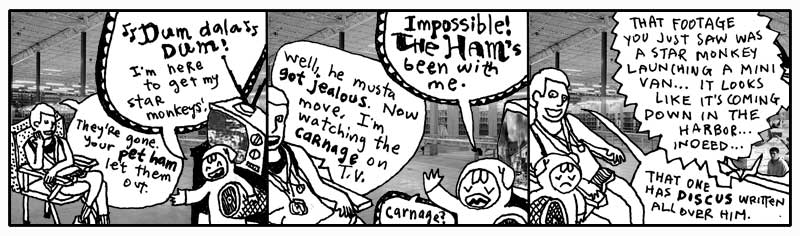
\includegraphics[width=1.0\textwidth]{cache/31.png}
\newpage
\thispagestyle{empty}
\mbox{}
\cleartooddpage


\chapter{Them What Make the Rules and Them What Live the Dream}
\vfill
\begin{center}
  
\includegraphics{cache/chapterpoignantguide5.png}
\end{center}
\vspace{2cm}
\newpage
\thispagestyle{empty}
\mbox{}
\clearpage
	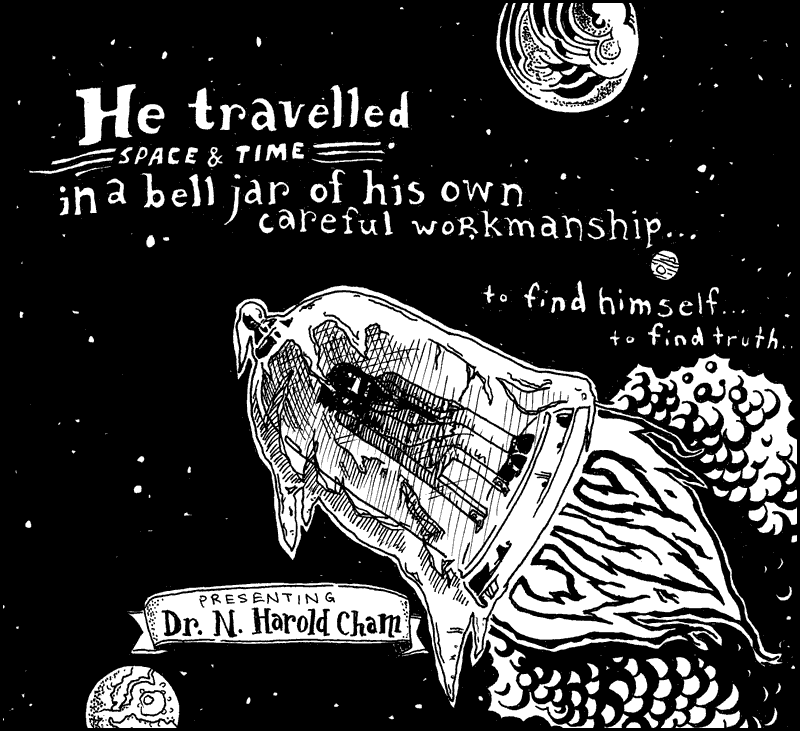
\includegraphics[width=1.0\textwidth]{cache/32.png}

Frankly, I'm sick and tired of hearing that Dr. Cham was a madman.
Yes, he tried to bury himself alive.  Yes, he electrocuted his niece.
Yes, in fact, he did dynamite a retirement home.  But this was all
with good cause and, in each case, I believe he took the correct
course of action.

I'm sure you'd like to side with popular opinion, but you're bound to
feel some small trickle of admiration for him once he's taken time to
teach you all about Ruby's class definitions. And moreso when you
learn about mixins.  And perhaps, by the end of the chapter, we can
all start to look beyond the Doctor's grievous past and stop calling
him a madman.

So if you need to call him a madman, I'd start heading down to the
train tracks to smash up some long flourescent light bulbs.  Get it
out of your system right now, before we dig in.


\section{This One's For the Disenfranchised}


	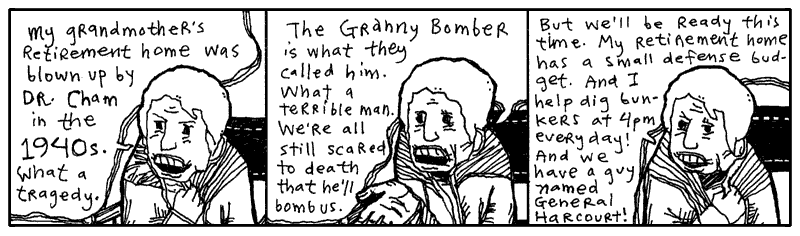
\includegraphics[width=1.0\textwidth]{cache/33.png}

If you give me a number, which is any year from Dr. Cham's life, I'll
give you a synopsis of that time period.  And I'll do it as a Ruby
method, so it's an independent piece, an isolated chunk of code which
can be hooked up to the voice of a robotic volcano, when such a thing
becomes the apex of authoritative voice talents.

Okay, so I need you to notice \lstinline[breaklines=true]|def| and
\lstinline[breaklines=true]|case| and
\lstinline[breaklines=true]|when|.  You've seen the Ranges, the closed
accordions of \lstinline[breaklines=true]|1895..1913|, back in chapter
3.  They contain both ends and in between.  And the backslashes at the
end of each line simply ignore the {\em Enter} key at the end of each
line, assuring Ruby that there is {\em more of this line to come}.

So, please: \lstinline[breaklines=true]|def| and
\lstinline[breaklines=true]|case| and
\lstinline[breaklines=true]|when|.


\begin{lstlisting}[basicstyle=\ttfamily\color{basiccolor},
    commentstyle = \ttfamily\color{commentcolor},
    keywordstyle=\ttfamily\color{keywordscolor},
    stringstyle=\color{stringcolor},
    language=Ruby,
    basicstyle=\small\ttfamily,
    showstringspaces=false,
  ]

 def dr_chams_timeline( year )
   case year
   when 1894
     "Born."
   when 1895..1913
     "Childhood in Lousville, Winston Co., Mississippi."
   when 1914..1919
     "Worked at a pecan nursery; punched a Quaker."
   when 1920..1928
     "Sailed in the Brotherhood of River Wisdomming, which journeyed \
      the Mississippi River and engaged in thoughtful self-improvement, \
      where he finished 140 credit hours from their Oarniversity."
   when 1929
     "Returned to Louisville to pen a novel about time-travelling pheasant \
      hunters."
   when 1930..1933
     "Took up a respectable career insuring pecan nurseries.  Financially \
      stable, he spent time in Brazil and New Mexico, buying up rare paper-shell \
      pecan trees.  Just as his notariety came to a crescendo: gosh, he tried to \
      bury himself alive."
   when 1934
     "Went back to writing his novel.  Changed the hunters to insurance tycoons \
      and the pheasants to Quakers."
   when 1935..1940
     "Took Arthur Cone, the Headmaster of the Brotherhood of River Wisdomming, \
      as a houseguest.  Together for five years, engineering and inventing."
   when 1941
     "And this is where things got interesting."
   end
 end

\end{lstlisting}


The \lstinline[breaklines=true]|def| keyword.  Here is our first {\bf
  method definition}.  A plain kernel method, which can be used
anywhere in Ruby.  And how do we run it?


\begin{lstlisting}[basicstyle=\ttfamily\color{basiccolor},
    commentstyle = \ttfamily\color{commentcolor},
    keywordstyle=\ttfamily\color{keywordscolor},
    stringstyle=\color{stringcolor},
    language=Ruby,
    basicstyle=\small\ttfamily,
    showstringspaces=false,
  ]

 puts dr_chams_timeline( 1941 )

\end{lstlisting}


Which answers with ``And this is where things got interesting.''  It's
the same story again and again: {\em use your answers.}  I've set
things up above so that the \lstinline[breaklines=true]|case|
statement always answers with a string. And since the case statement
is the final (and only) statement in the method, then the method
answers with that string.  Trickling water spilling down from ledge to
ledge.

Let me be clear about the \lstinline[breaklines=true]|case| statement.
Actually, I should call it a \lstinline[breaklines=true]|case..when|
statement, since they cannot be used separately.  The
\lstinline[breaklines=true]|case| keyword is followed by a value,
which is compared against each of the values which follow
\lstinline[breaklines=true]|when| keywords.  The first value to
qualify as a match is the one the case uses and the rest are ignored.
You can do the same thing with a bunch of
\lstinline[breaklines=true]|if..elsif| statements, but it's wordier.


\begin{lstlisting}[basicstyle=\ttfamily\color{basiccolor},
    commentstyle = \ttfamily\color{commentcolor},
    keywordstyle=\ttfamily\color{keywordscolor},
    stringstyle=\color{stringcolor},
    language=Ruby,
    basicstyle=\small\ttfamily,
    showstringspaces=false,
  ]

 case year
 when 1894
   "Born."
 when 1895..1913
   "Childhood in Lousville, Winston Co., Mississippi."
 else
   "No information about this year."
 end

\end{lstlisting}


Is identical to:


\begin{lstlisting}[basicstyle=\ttfamily\color{basiccolor},
    commentstyle = \ttfamily\color{commentcolor},
    keywordstyle=\ttfamily\color{keywordscolor},
    stringstyle=\color{stringcolor},
    language=Ruby,
    basicstyle=\small\ttfamily,
    showstringspaces=false,
  ]

 if 1894 === year
   "Born."
 elsif 1895..1913 === year
   "Childhood in Lousville, Winston Co., Mississippi."
 else
   "No information about this year."
 end

\end{lstlisting}


The {\bf triple equals} is a length of velvet rope, checking values
much like the double equals.  It's just: the triple equals is a longer
rope and it sags a bit in the middle.  It's not as strict, it's a bit
more flexible.

Take the Ranges above.  \lstinline[breaklines=true]|(1895..1913)|
isn't at all {\bf equal} to \lstinline[breaklines=true]|1905|.  No,
the Range \lstinline[breaklines=true]|(1895..1913)| is only truly {\bf
  equal} to any other Range \lstinline[breaklines=true]|(1895..1913)|.
In the case of a Range, the triple equals cuts you a break and lets
the Integer \lstinline[breaklines=true]|1905| in, because even though
it's not {\bf equal} to the Range, it's {\bf included} in the set of
Integers represented by the Range.  Which is good enough in some
cases, such as the timeline I put together earlier.

Which actually looked like a timeline, didn't it?  I mean, sure,
\lstinline[breaklines=true]|dr_chams_timeline| method is code, but it
does read like a timeline, clean and lovely.

\newpage

	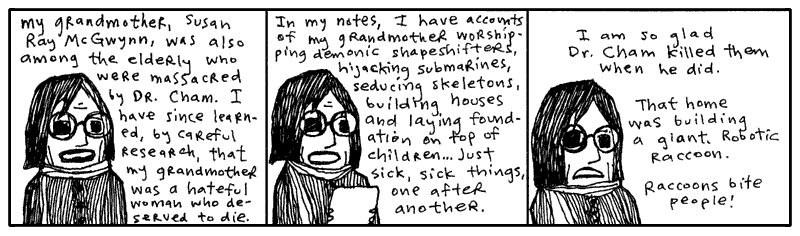
\includegraphics[width=1.0\textwidth]{cache/34.png}


\subsection{But Was He Sick??}



You know, he had such bad timing.  He was scattered as a novelist, but
his ventures into alchemy were very promising.  He had an elixir of
goat's milk and sea salt that got rid of leg aches. One guy even grew
an inch on a thumb he'd lost.  He had an organic health smoke that
smelled like foot but gave you night vision.  He was working on
something called Liquid Ladder, but I've never seen or read anything
else about it.  It can't have been for climbing.  Who knows.

One local newspaper actually visited Dr. Cham.  Their book reviewer
gave him four stars. Really.  She did an article on him.  Gave him a
rating.

Just know that Dr. N. Harold Cham felt terrible about his niece.  He
felt the shock treatment would work.  The polio probably would have
killed her anyway, but he took the chance.

On Sept. 9, 1941, after sedating her with a dose of phenacetin in his
private operating room, he attached the conducting clips to Hannah's
nose, tongue, toes, and elbows.  Assisted by his apprentice, a
bespeckled undergraduate named Marvin Holyoake, they sprinkled the
girl with the flakes of a substance the doctor called {\em opus
  magnum}.  A white powder gold which would carry the current and
blatantly energize the girl, forcing her blood to bloom and fight and
vanquish.

But how it failed, oh, and how, when the lever was tossed, she arched
and kicked -- and {\bf KABLAM!} -- and {\bf BLOY-OY-OY-KKPOY!}
Ringlets of hair and a wall of light, and the bell of death rang.  The
experiment collapsed in a dire plume of smoke and her innocence ({\em
  for weeks, everyone started out with, ``And she will never have the
  chance...''}) was a great pit in the floor and in their lungs.

To Hannah, I code.


\begin{lstlisting}[basicstyle=\ttfamily\color{basiccolor},
    commentstyle = \ttfamily\color{commentcolor},
    keywordstyle=\ttfamily\color{keywordscolor},
    stringstyle=\color{stringcolor},
    language=Ruby,
    basicstyle=\small\ttfamily,
    showstringspaces=false,
  ]

 opus_magnum = true
 def save_hannah
   success = opus_magnum
 end

\end{lstlisting}


A method is its own island.  And what goes on inside is unaffected by
the simple variables around it. Dr. Cham couldn't breach the illness
of his niece, no more than an \lstinline[breaklines=true]|opus_magnum|
variable can penetrate the steely exterior of a method.

Should we run the \lstinline[breaklines=true]|save_hannah| method,
Ruby will squawk at us, claiming it sees no
\lstinline[breaklines=true]|opus_magnum|.

I'm talking about {\bf scope}.  Microscopes narrow and magnify your
vision.  Telescopes extend the range of your vision.  In Ruby, {\bf
  scope} refers to a field of vision inside methods and blocks.

A method's \lstinline[breaklines=true]|def| statement opens its
vision.  Variable names introduced there will be seen by the method
and kept meaningful until its \lstinline[breaklines=true]|end| closes
its eyes.  You can pass data into a method by using arguments and data
can be returned from the method, but the names used inside the method
are only good for its scope.

Some variables have wider scope.  Global variables like
\lstinline[breaklines=true]|$LOAD_PATH|, which start with a {\bf cash}
symbol, are available in any scope.  Instance variables like
\lstinline[breaklines=true]|@names|, which start with an {\bf at} are
available anywhere inside a class scope.  Same goes for class
variables like \lstinline[breaklines=true]|@@tickets|. Class and
instance variables will be explored in a moment.

Blocks have scope, but it's a bit fuzzier.  More flexible.


\begin{lstlisting}[basicstyle=\ttfamily\color{basiccolor},
    commentstyle = \ttfamily\color{commentcolor},
    keywordstyle=\ttfamily\color{keywordscolor},
    stringstyle=\color{stringcolor},
    language=Ruby,
    basicstyle=\small\ttfamily,
    showstringspaces=false,
  ]

 verb = 'rescued'
 ['sedated', 'sprinkled', 'electrocuted'].
 each do |verb|
   puts "Dr. Cham " + verb + " his niece Hannah."
 end
 puts "Yes, Dr. Cham " + verb + " his niece Hannah."

\end{lstlisting}


The block {\em iterates} (spins, cycles) through each of the Doctor's
actions.  The \lstinline[breaklines=true]|verb| variable changes with
each pass.  In one pass, he's sedating.  In the next, he's powdering.
Then, he's electrocuting.

So, the question is: after the block's over, will he have rescued
Hannah?


\begin{lstlisting}[basicstyle=\ttfamily\color{basiccolor},
    commentstyle = \ttfamily\color{commentcolor},
    keywordstyle=\ttfamily\color{keywordscolor},
    stringstyle=\color{stringcolor},
    language=Ruby,
    basicstyle=\small\ttfamily,
    showstringspaces=false,
  ]

 Dr. Cham sedated his niece Hannah.
 Dr. Cham sprinkled his niece Hannah.
 Dr. Cham electrocuted his niece Hannah.
 Yes, Dr. Cham electrocuted his niece Hannah.

\end{lstlisting}


Blocks are allowed to see variables in the vicinity.  The block
noticed that the \lstinline[breaklines=true]|verb| variable existed
and it overwrote its contents as it went along.  When the block
completed and its tiny life ended, the
\lstinline[breaklines=true]|verb| variable came out a changed
creature.

If a block uses a variable which hasn't been used previously, though,
then that variable vanishes at the end of the block.  The block's {\bf
  scope} closes and the variable goes with it.  Say that
\lstinline[breaklines=true]|verb| wasn't used before the block.


\begin{lstlisting}[basicstyle=\ttfamily\color{basiccolor},
    commentstyle = \ttfamily\color{commentcolor},
    keywordstyle=\ttfamily\color{keywordscolor},
    stringstyle=\color{stringcolor},
    language=Ruby,
    basicstyle=\small\ttfamily,
    showstringspaces=false,
  ]

 ['sedated', 'powdered', 'electrocuted'].
 each do |verb|
   puts "Dr. Cham " + verb + " his niece Hannah."
 end
 puts "Yes, Dr. Cham " + verb + " his niece Hannah."

\end{lstlisting}


Pulls an error: 
\lstinline[breaklines=true]|undefined local variable or method `verb'|.  
Poof.

It must be something difficult, even for a great scientist, to carry
away the corpse of a young girl whose dress is still starched and
embroidered, but whose mouth is darkly clotted purple at the corners.
In Dr. Cham's journal, he writes that he was tormented by her ghost,
which glistened gold and scorched lace.  His delusions grew and he ran
from hellhounds and massive vengeful, angelic hands.

Only weeks later, he was gone, propelled from these regrets, vanishing
in the explosion that lifted him from the planet.

And even as you are reading this now, sometime in these moments, the
bell jar craft of our lone Dr. Cham touched down upon a distant planet
after a sixty year burn.  As the new world came into view, as the
curvature of the planet widened, as the bell jar whisked through the
upset heavens, tearing through sheets of aurora and solar wind,
Dr. Cham's eyes were shaken open.

	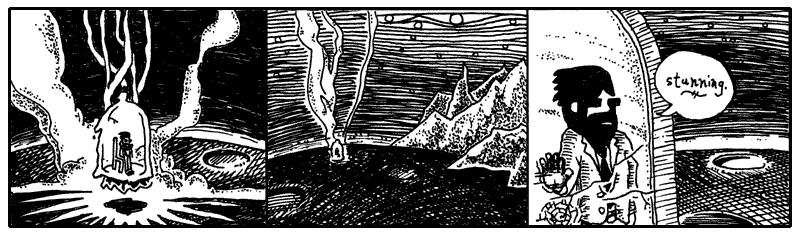
\includegraphics[width=1.0\textwidth]{cache/35.png}

What you are witnessing is the landing of Dr. Cham on the planet
Endertromb.  From what I can gather, he landed during the cusp of the
Desolate Season, a time when there really isn't much happening on the
planet.  Most of the inhabitants find their minds locked into a
listless hum which causes them to disintegrate into just vapid ghosts
of one-part-wisdom and three-parts-steam for a time.

My modest grasp of the history and climate of Endertromb has been
assembled from hanging around my daughter's organ instructor, who grew
up on the planet.

	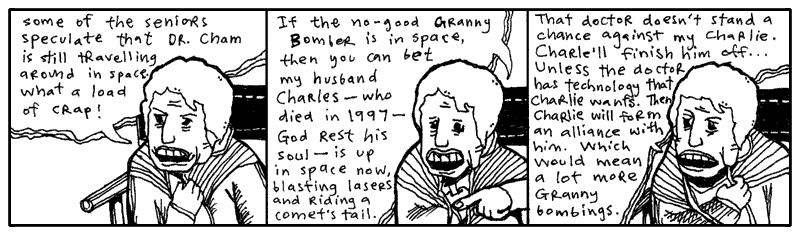
\includegraphics[width=1.0\textwidth]{cache/36.png}

I frequently drill my daughter's organ instructor in order to ensure
that he can keep appointments adequately.  That he can take house
calls at odd hours and promptly answer emergency calls. When he
finally revealed to me that he was an alien whose waking day consisted
of five-hundred and forty waking hours, I was incredibly elated and
opened a contractual relationship with him which will last into 2060.

For three days (by his pocket watch's account), Dr. Cham travelled the
dark shafts of air, sucking the dusty wind of the barren planet. But
on the third day, he found the Desolate Season ending and he awoke to
a brilliant vista, decorated with spontaneous apple blossoms and dewy
castle tiers.


\section{A Castle Has Its Computers}


	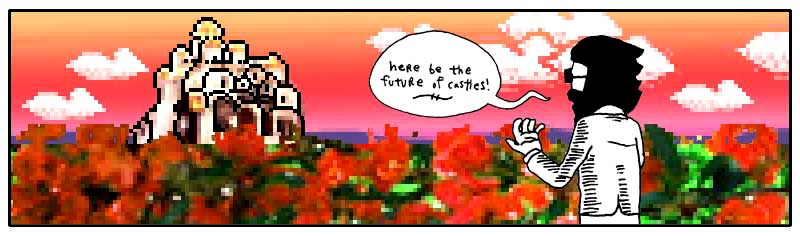
\includegraphics[width=1.0\textwidth]{cache/37.png}

Our intrepid Doctor set off for the alien castle, dashing through the
flowers.  The ground belted past his heels.  The castle inched up the
horizon.  He desired a stallion, but no stallion appeared.  And that's
how he discovered that the planet wouldn't read his mind and answer
his wishes.

As my daughter's organ instructor explained it, however, the planet
{\bf could read minds} and it {\bf could grant wishes}.  Just not both
at the same time.

One day as I quizzed the organ maestro, he sketched out the following
Ruby code on a pad of cheese-colored paper.  (And queer cheese smells
were coming from somewhere, I can't say where.)


\begin{lstlisting}[basicstyle=\ttfamily\color{basiccolor},
    commentstyle = \ttfamily\color{commentcolor},
    keywordstyle=\ttfamily\color{keywordscolor},
    stringstyle=\color{stringcolor},
    language=Ruby,
    basicstyle=\small\ttfamily,
    showstringspaces=false,
  ]

 require 'endertromb'
 class WishMaker
   def initialize
     @energy = rand( 6 )
   end
   def grant( wish )
     if wish.length > 10 or wish.include? ' '
       raise ArgumentError, "Bad wish."
     end
     if @energy.zero?
       raise Exception, "No energy left."
     end
     @energy -= 1
     Endertromb::make( wish )
   end
 end

\end{lstlisting}


This is the wish maker.

Actually, no, this is a {\bf definition for a wish maker.}  To Ruby,
it's a {\bf class definition}. The code describes how a certain {\bf
  object} will work.

Each morning, the wish maker starts out with up to five wishes
available for granting. A new \lstinline[breaklines=true]|WishMaker|
is created at sun up.


\begin{lstlisting}[basicstyle=\ttfamily\color{basiccolor},
    commentstyle = \ttfamily\color{commentcolor},
    keywordstyle=\ttfamily\color{keywordscolor},
    stringstyle=\color{stringcolor},
    language=Ruby,
    basicstyle=\small\ttfamily,
    showstringspaces=false,
  ]

 todays_wishes = WishMaker.new

\end{lstlisting}


The \lstinline[breaklines=true]|new| method is a class method which
creates a new, blank object.  It also calls the object's
\lstinline[breaklines=true]|initialize| method automatically.  In the
\lstinline[breaklines=true]|WishMaker| definition, you'll see the
\lstinline[breaklines=true]|initalize| method, which contains a single
line of code: \lstinline[breaklines=true]|@energy = rand( 6 )|.

The \lstinline[breaklines=true]|rand( 6 )| picks a number between 0
and 5.  This number will represent the number of wishes left in the
day.  So, occassionally there are no wishes available from the wish
maker.

The random number is assigned to an {\bf instance variable} which is
named \lstinline[breaklines=true]|@energy|. This instance variable
will be available any time throughout the class.  The variable can't
be used outside the {\bf scope} of the class.

In chapter three, we briefly looked at instance variables and decided
to respect them as {\bf attributes}.  (The {\bf at symbol} could mean
{\bf attribute}.)  Instance variables can used to store any kind of
information, but they're most often use to store bits of information
about the object represented by the class.

In the above case, each wish maker for the day has its own energy
level.  If the wish maker were a machine, you might see a gauge on it
that points to the energy left inside. The
\lstinline[breaklines=true]|@energy| instance variable is going to act
as that gauge.


\begin{lstlisting}[basicstyle=\ttfamily\color{basiccolor},
    commentstyle = \ttfamily\color{commentcolor},
    keywordstyle=\ttfamily\color{keywordscolor},
    stringstyle=\color{stringcolor},
    language=Ruby,
    basicstyle=\small\ttfamily,
    showstringspaces=false,
  ]

 todays_wishes = WishMaker.new 
 todays_wishes.grant( "antlers" )

\end{lstlisting}


Okay, step back and ensure you understand the example here.  The
\lstinline[breaklines=true]|WishMaker| class is an outline we've laid
out for how the whole magic wish program works.  It's not the {\em
  actual} genie in the bottle, it's the paperwork behind the scenes.
It's the rules and obligations the genie has to live by.

It's \lstinline[breaklines=true]|todays_wishes| that's the genie in
the bottle.  And here we're giving it a wish to grant. Give us
antlers, genie.  (If you really get antlers from this example, I don't
want to hear about it.  Go leap in meadows with your own kind now.)

In the last chapter, the drill was: Ruby has two halves.

\begin{enumerate}
\item Defining things.
\item Putting those things into action.
\end{enumerate}

What are the actions in Ruby?  Methods.  And now, you're having a lick
of the definition language built-in to Ruby.  Method definitions using
\lstinline[breaklines=true]|def|.  Class definitions using
\lstinline[breaklines=true]|class|.

At this point in your instruction, it's easier to understand that {\bf
  everything in Ruby is an object.}


\begin{lstlisting}[basicstyle=\ttfamily\color{basiccolor},
    commentstyle = \ttfamily\color{commentcolor},
    keywordstyle=\ttfamily\color{keywordscolor},
    stringstyle=\color{stringcolor},
    language=Ruby,
    basicstyle=\small\ttfamily,
    showstringspaces=false,
  ]

 number = 5
 print number.next                  # prints '6'

 phrase = 'wishing for antlers'
 print phrase.length                # prints '19'

 todays_wishes = WishMaker.new
 todays_wishes.grant( "antlers" )

\end{lstlisting}


And, consequently, each object has a class behind the scenes.


\begin{lstlisting}[basicstyle=\ttfamily\color{basiccolor},
    commentstyle = \ttfamily\color{commentcolor},
    keywordstyle=\ttfamily\color{keywordscolor},
    stringstyle=\color{stringcolor},
    language=Ruby,
    basicstyle=\small\ttfamily,
    showstringspaces=false,
  ]

 print 5.class                       # prints 'Integer'
 print 'wishing for antlers'.class   # prints 'String'
 print WishMaker.new.class           # prints 'WishMaker'

\end{lstlisting}


Dr. Cham never saw the wish maker as he hustled across the
landspace. It lay far beyond his landing in the valley of Sedna.  Down
sheer cliffs stuffed with layers of thicket, where you might toss your
wish (written on a small 1" x 6" slip), down into the gaping void.
Hopefully it will land on a lizard's back, sticking to its spindly
little horn.

And let's say your wish makes it that far.  Well, then, {\em down the
  twisted wood} goes the skinny salamander, scurrying through the
decaying churches which had been {\bf pushed} over that steep canyon
ledge once and for all.  And the expired priest inside, {\em who
  weathered the fall} as well, will kill the little amphibian --
strangle it to death with a blessed gold chain -- and save it for the
annual {\em Getting To Know You} breakfast.  He'll step on your
precious little wish and, when the {\bf thieves come}, that slip will
still be there, stuck on his sole.  Of course, the thieves' {\bf
  preferred method of torture} is to cut a priest in thin deli-shaved
slices {\em from top to bottom}.  Who can cull evidence from that?
And when they chop that last thin slice of shoe sole, they'll have
that {\bf rubber scalp} in hand for {\em good luck} and {\em good
  times}. But they {\bf canoe} much too hard, these thieves.  They
slap their paddles swiftly in the current to get that great {\em
  outboard motor mist} going.  But the shoe sole is {\em on a weak
  chain}, tied to one man's belt.  And a {\bf hairy old carp} {\em
  leaps, latches} on to that minute fraction of footwear.  And the
thieves {\em can try}, but they don't see {\em underwater}.  If they
could, they'd see that {\bf mighty cable}, packed with millions of
{\em needly} fiber optics.  Indeed, {\bf that fish is a peripheral
  plugged} right into the {\em core workings} of the planet
Endertromb.  {\bf All it takes is one swallow} from that fish {\bf and
  your wish is home free!}

And that's how wishes come true for children in this place.

Once my daughter's organ instructor had drawn up the class for the
wish maker, he then followed with a class for the planet's mind
reader.


\begin{lstlisting}[basicstyle=\ttfamily\color{basiccolor},
    commentstyle = \ttfamily\color{commentcolor},
    keywordstyle=\ttfamily\color{keywordscolor},
    stringstyle=\color{stringcolor},
    language=Ruby,
    basicstyle=\small\ttfamily,
    showstringspaces=false,
  ]

 require 'endertromb'
 class MindReader
   def initialize
     @minds = Endertromb::scan_for_sentience
   end
   def read
     @minds.collect do |mind|
        mind.read
     end
   end
 end

\end{lstlisting}


Much as you've seen before, the \lstinline[breaklines=true]|initalize|
happens when a new \lstinline[breaklines=true]|MindReader| object is
created. This \lstinline[breaklines=true]|initialize| gathers scans
the planet for mindshare.  It looks like these minds are stored in an
array, since they are later iterated over using the
\lstinline[breaklines=true]|collect| method.

Both the wish maker and the mind reader refer to a class named
\lstinline[breaklines=true]|Endertromb|.  This class is stored in a
file \lstinline[breaklines=true]|endertromb.rb|, which is loaded with
the code: \lstinline[breaklines=true]|require 'endertromb'|. Often
you'll use other classes to accomplish part of your task.  Most of the
latter half of this book will explore the wide variety of helpful
classes that can be loaded in Ruby.



\subsection{Dr. Cham Ventures Inside}



But as Dr. Cham neared the castle, although the planet was aware of
his thoughts, sensing his wonderment and anticipation, all Dr. Cham
felt was deadness.  He tromped up the steps of its open gate and
through the entrance of the most beautiful architecture and was almost
certain it was deserted.

For a while he knocked.  Which paid off.


He watched the baby whale rise like a determined balloon.  He
marvelled at his first alien introduction and felt some concern that
it had passed so quickly.  Well, he would wait inside.

As he stepped through the castle door, he felt fortunate that the door
hadn't been answered by a huge eagle with greedy talons, eager to
play.  Or a giant mouse head.  Or even a man-sized hurricane.  Just a
tubby little choo-choo whale.

``Not a place to sit down in this castle,'' he said.

At first, he had thought he had just entered a very dim hallway, but
as his eyes adjusted, he saw the entrance extended into a tunnel.  The
castle door had opened right into a passage made of long, flat slabs
of rock.  Some parts were congruous and resembled a corridor.  Other
parts narrowed, and even tilted, then finally tipped away out of view.

The passage was lit by small doorless refrigerators, big enough to
hold an armful of cabbage, down by his feet.  He peered inside one,
which was hollow, illuminated along all sides, and turning out ice
shards methodically.

He pawed the ice chips, which clung dryly to his fingertips, and he
scrubbed his hands in the ice.  Which left some muddy streaks on his
hands, but satisfied a small part of his longing to bathe. How long
had it been?  Ten years?  Thirty?

Along the passage, long tubes of cloth cluttered some sections.
Later, bright pixel matter in porcelain scoops and buckets.

He happened upon a room which had been burrowed out of the tunnel
which had a few empty turtle shells on the ground and a large
illuminated wall.  He stared into the room, bewildered.  What could
this be?  In one state of mind, he thought of having a seat on a
shell.  This could be the entrace at last, some kind of receiving
room.  On the other hand, spiders could pour out of the shell's hollow
when he sat.  He moved on.



\subsection{Meal in a Castle's Pocket}



As he journeyed along the passageways (for the central tunnel forked
and joined larger, vacuous caverns), he picked up themes in some
locations.  Groups of rooms infested with pumping machinery.  Cloth
and vats of glue dominated another area.  He followed voices down a
plush, pillowed cavity, which led him to a dead end: a curved wall
with a small room carved at eye-level.

He approached the wall and, right in the cubby hole, were two
aardvarks eating at a table.

They gazed at him serenely, both munching on some excavated beetle
twice their size, cracked open and frozen on its back on the table.

``Hello, little puppets,'' he said, and they finished their bites and
kept looking with their forks held aloof.

``I wish my niece Hannah were here to meet you,'' he told the
attentive miniature aardvarks.  ``She'd think you were an intricate
puppet show.''  He peered in at the dining area, shelves with sets of
plates, hand towels.  Half of a tiny rabbit was jutting out from the
top a machine, creamy red noodles were spilling out underneath it.  A
door at the back of the room hung ajar.  Dr. Cham could see a
flickering room with chairs and whirring motors through the door.

``Any child would want this dollhouse,'' he said.  ``Hannah, my niece,
as I mentioned, she has a wind-up doll that sits at a spindle and
spins yarn.  It's an illusion, of course.  The doll produces no yarn
at all.''

One of the aardvarks opened a trapdoor in the floor and pressed a
button down inside, which lit. Then, a small film projector slowly
came up on a rod.  The other aardvark sat and watched Dr. Cham.

``But Hannah still reaches down into the dollhouse and collects all
the imaginary yarn into a bundle.  Which she takes to her mother, my
sister, who is very good at humoring Hannah. She sews a dress to the
doll's dimensions, which Hannah takes back to the doll.''

``And she tells the doll, `Here, look, your hard work and
perserverance has resulted in this beautiful dress. You can now accept
the Chief of Police's invitation to join him tonight at the Governor's
Mansion.'  And she has a doll in a policeman's uniform who plays the
part of the Chief.  He's too scrawny to be an actual Chief, that would
require quite a bit of plastic.''

The aardvark responsible for the film projector loaded a reel and
aimed the projector at the back wall.  The film spun to life and the
aardvark took a seat.  A green square appeared on the wall.  The
attentive aardvark stared at Dr. Cham still.

``Your films are coloured,'' said Dr. Cham.  ``What a lovely, little
life.''

The film played on: a blue square.  Then, a red circle.  Then, an
orange square.  The attentive aardvark turned away, watched the screen
change to a pink triangle, and both aardvarks resumed eating.

A purple star.  A red square.  With quietness settling, Dr. Cham could
hear notes droning from the projector.  Like a slow, plodding music
box trying to roll its gears along the train tracks.

``Yes, enjoy your supper,'' said Dr. Cham and he politely tipped his
head away, marching back up the path he'd taken.



\subsection{Another Dead End Where Things Began}



He found himself lost in the castle's tunnels.  Nothing looked
familiar.  He wasn't worried much, though.  He was on another planet.
He would be lost regardless.

He wound through the tunnels, attempting to recall his paths, but far
too interested in exploring to keep track of his steps.  He followed a
single tunnel deep, down, down, which slanted so steeply that he had
to leap across ledges and carefully watch his footholds. The gravity
here seemed no different than Earth.  His legs were pulled into slides
just as easily.

Although he had no absolute way of knowing where he was, he felt
certain that he had left the castle's boundaries.  This deep, this
long of a walk.  It had been an hour since he'd entered through the
door.  And, as the tunnel wound back up, he was sure that he would
emerge into a new dwelling, perhaps even a manhole which he could peek
out from and see the castle.  Perhaps he shouldn't have come so far
down this route.  He hoped nothing was hibernating down here.

The tunnel came to a stop.  A dark, dead end.

	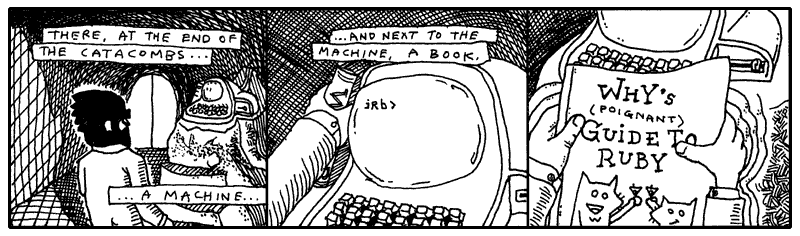
\includegraphics[width=1.0\textwidth]{cache/39.png}

He had time.  So he read the book.  He read of the foxes and their
pursuit of the porcupine who stole their pickup truck.  He read of the
elf and the ham.  He saw the pictographs of himself and found he could
really relate to his own struggles.  He even learned Ruby.  He saw how
it all ended.

Were I him, I couldn't have stomached it.  But he did.  And he pledged
in his bosom to see things out just as they happened.

On the computer monitor, Dr. Cham saw the flashing
\lstinline[breaklines=true]|irb| prompt.  Like Dr. Cham, you might
recognize the \lstinline[breaklines=true]|irb| prompt from The Tiger's
Vest (the first expansion pak to this book, which includes a basic
introduction to Interactive Ruby.)

Whereas he had just been exploring tunnels by foot, he now explored
the machine's setup with the prompt.  He set the book back where he
had found it.  He didn't need it anymore.  This was all going to
happen whether he used it or not.

He started with:


\begin{lstlisting}

 irb> Object::constants
   => ["Marshal", "String", "Dir", "LoadError", "Float", ... and so on ]

\end{lstlisting}


This command lists all the top-level constants.  Classes are also
listed as constants, so this list can be great to see what's loaded
into Ruby at any time.

He scanned the list for anything unfamiliar.  Any classes which didn't
come with Ruby. \lstinline[breaklines=true]|Marshal|,
\lstinline[breaklines=true]|String|, \lstinline[breaklines=true]|Dir|,
\lstinline[breaklines=true]|LoadError|,
\lstinline[breaklines=true]|Float|.  Each of those came with Ruby.

But further down the list:


\begin{lstlisting}

 ... "Struct", "Values", "Time", "Elevator", "Range" ...

\end{lstlisting}


{\em Elevator?}  Exactly the kind of class to poke around with.  He
had a go.


\begin{lstlisting}

 irb> Elevator::methods
   => ["method", "freeze", "allocate", ... another long list ... ]
 irb> Elevator::class_variables
   => ['@@diagnostic_report', '@@power_circuit_active', '@@maintenance_password']
 irb> Elevator::constants
   => []

\end{lstlisting}


Looks like the \lstinline[breaklines=true]|Elevator| class had plenty
of methods.  Most of these looked like they were the same methods
every object has in Ruby.  For example,
\lstinline[breaklines=true]|method|,
\lstinline[breaklines=true]|freeze| and
\lstinline[breaklines=true]|allocate| come with every class in Ruby.
(\lstinline[breaklines=true]|Elevator::freeze| would keep the
\lstinline[breaklines=true]|Elevator| class from being changed.
\lstinline[breaklines=true]|Elevator::allocate| would make a new
\lstinline[breaklines=true]|Elevator| object without calling the
\lstinline[breaklines=true]|initialize| method.)

The \lstinline[breaklines=true]|class_variables| were interesting to
Dr. Cham.  This elevator appeared genuine. But no available
\lstinline[breaklines=true]|constants|.  This tells us there are no
classes nested inside the \lstinline[breaklines=true]|Elevator| class.

He tried to create an \lstinline[breaklines=true]|Elevator| object.


\begin{lstlisting}

 irb> e = Elevator::new
 ArgumentError: wrong number of arguments (0 for 1), requires a password
         from (irb):2:in `initialize'
         from (irb):2:in `new'
         from (irb):2
         from :0

\end{lstlisting}


He tried a few passwords.


\begin{lstlisting}

 irb> e = Elevator::new( "going up" )
 AccessDeniedError: bad password
 irb> e = Elevator::new( "going_up" )
 AccessDeniedError: bad password
 irb> e = Elevator::new( "stairs_are_bad" )
 AccessDeniedError: bad password
 irb> e = Elevator::new( "StairsAreBad" )
 AccessDeniedError: bad password

\end{lstlisting}


That was useless.  {\em Oh, wait!}  The maintenance password.  Listed
in the \lstinline[breaklines=true]|class_variables|.


\begin{lstlisting}

 irb> Elevator::maintenance_password
 NoMethodError: undefined method `maintenance_password' for Elevator:Class
         from (irb):1
         from :0

\end{lstlisting}


Hmm.  Instance variables are only available inside an object.  And
class variables are only available inside a class.  How to get at that
password?


\begin{lstlisting}

 irb> class Elevator
 irb>   def Elevator.maintenance_password
 irb>     @@maintenance_password
 irb>   end
 irb> end
   => nil
 irb> Elevator::maintenance_password
   => "stairs_are_history!"

\end{lstlisting}


Alright!  He got the password.  Did you see that?

He added a class method to the \lstinline[breaklines=true]|Elevator|
class.  Isn't that great how you can start a new class definition for
\lstinline[breaklines=true]|Elevator| and Ruby just adds your changes
to the existing class definition?

Class methods are usually called with the {\bf double colon}.  But, a
period is fine as well. Since \lstinline[breaklines=true]|Elevator| is
a class itself, Ruby will figure that if you call
\lstinline[breaklines=true]|Elevator.maintenance_password|, you're
calling a class method.  The double colon simply helps make class
methods obvious to the reader.

And justly so.  Class methods are a bit unusual.  Normally you won't
want to store information directly inside of a class.  However, if you
have a bit of information that you need to share among all objects of
a class, then you have a good reason to use the class for
storage. It's understandable that the
\lstinline[breaklines=true]|@@maintenance_password| would be stored in
the class, instead of in each separate object.  This way, the objects
can simply reach up into the class and see the shared password.

Here's probably how the password protection works.


\begin{lstlisting}[basicstyle=\ttfamily\color{basiccolor},
    commentstyle = \ttfamily\color{commentcolor},
    keywordstyle=\ttfamily\color{keywordscolor},
    stringstyle=\color{stringcolor},
    language=Ruby,
    basicstyle=\small\ttfamily,
    showstringspaces=false,
  ]

 class Elevator
   def initialize( pass )
     raise AccessDeniedError, "bad password" \
       unless pass.equals? @@maintenance_password
   end
 end

\end{lstlisting}


Passwording a class like this is pointless, since anything in Ruby can
be altered and overwritten and remolded.  Dr. Cham had the password
and ownership of the elevator is his.


\begin{lstlisting}

 irb> e = Elevator.new( "stairs_are_history!" )
 #<Elevator:0x81f12f4 @level=4>
 irb> e.level = 1

\end{lstlisting}


Dr. Cham was standing right there when the elevator doors, off behind
the computer terminal, opened for him.  With an exasperated sense of
accomplishment and a good deal of excitement surrounding all of the
events that lie ahead, he stepped into the elevator and pressed 4.

\newpage


\section{The Continued Story of My Daughter's Organ \mbox{Instructor}}


I know you may be alarmed to hear that I have a daughter.  You think
my writing is indicative of a palsied or infantile mind.  Well, please
rest.  I don't have a daughter. But I can't let that stop me from
sorting out her musical training.

As I was related these elaborate histories of the planet Endertromb, I
found myself wandering through hallways, running my fingertips along
the tightly buttoned sofas and soaking myself in the saturated
bellowings of the pipes, as played by my daughter's organ instructor.
His notes resounded so deep and hollow in the walls of his manor that
I began to casually mistake them for an ominous silence, and found it
even easier to retreat into deep space with my thoughts.  To think
upon the ancient planet and its darker philosophies: its flesh
temples, tanned from the dermal remains of its martyrs; its whale
cartels, ingesting their enemies and holding them within for decades,
dragging them up and down the staircases of ribs; its poison fogs and
its painful doorways; and, the atrocious dynasties of The Originals,
the species which claims fathership to all of the intellegent beings
across the universe.

But, eventually, I'd hear those pipes of a higher octave sing and I'd
be back in the very same breezy afternoon where I'd left.

How interesting that even the breeze of our planet is quite a strange
thing to some outsiders.  For he had also told me of the travellers
from Rath-d, who ventured to Earth five centuries ago, but quickly
dissipated in our air currents since they and their crafts and their
armor were all composed of charcoal.

I had sat at the organ, listening to his faint tales of his colony,
while he punctuated his symphonies to greater volumes and the story
would disappear for awhile, until the coda came back around. He spoke
of he and his brothers piling into the hollow of his mother's tail and
tearing the waxy crescent tissue from the inner wall.  Juicy and
spongy and syrupy soap which bleached their mouths and purged their
esophagus as it went down.  They chewed and chomped the stuff and it
foamed.  After they ate, they blew bubbles at each other, each bubble
filled with a dense foam, which they slept upon.  And early in the
morning, when mother opened her tail again, she watched serenely as
her babies lay cradled in the stew of dark meatballs and sweet, sticky
froth.

He spelled out all the tastes of Endertromb.  Of their salmon's
starchy organs, which cooked into a pasta, and its eyes which melted
into rich cream.  Of their buttermelon with tentacles. And he was just
beginning to appreciate the delicacies as a child, only to be lifted
from a schoolyard by a pair of upright pygmy elephants who reached at
him, through the heavens, and snatched upon his collar with a vast
length of crane.

They transplanted him on Earth, led him from their craft, trumpeting
their snouts loudly for the city of Grand Rapids to hear, then left,
weeping and embracing each other.

``But, strangely (em-pithy-dah), I learned upon, played upon
(pon-shoo) the organs on my home (oth-rea) planet,'' he said.

My daughter's organ instructor speaks these extra words you see in
parentheses.  Who knows if they are from his native tongue or if they
are his own soundful hiccups.  He keeps another relic from Endertromb
as well: he has twelve names.

``No, (wen-is-wen),'' he said.  ``I have one name (im-apalla) which is
said (iff) many-many different ways.''

I call him Paij-ree in the morning and Paij-plo in the later
evening. Since it is day as I write, I will call him Paij-ree here.



\subsection{Mumble-Free Earplugs}



	\parpic[r]{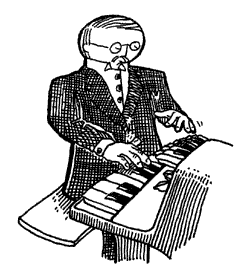
\includegraphics[width=0.3125\textwidth]{cache/40.png}}

So I told Paij-ree, ``Paij-ree, I am writing a book.  To teach the
world Ruby.''

``Oh, (pill-nog-pill-yacht) nice,'' he said.  He's known Ruby longer
than I have, but still: {\em I} will be my daughter's Ruby instructor.

And I said, ``Paij-ree, you are in the book.  And the stories of your
planet.''  I talk to him like he's E.T.  I don't know why.  Just like
how I said next, ``And then maybe someday you can go home to your mom
and dad!''

To which he said, ``(pon-shoo) (pon-shoo) (em-pithy-dah).''  Which is
his way of speaking out loud his silence and awe.

He wanted to see what I'd written, so I showed him this short method
I've written for you.


\begin{lstlisting}[basicstyle=\ttfamily\color{basiccolor},
    commentstyle = \ttfamily\color{commentcolor},
    keywordstyle=\ttfamily\color{keywordscolor},
    stringstyle=\color{stringcolor},
    language=Ruby,
    basicstyle=\small\ttfamily,
    showstringspaces=false,
  ]

 def wipe_mutterings_from( sentence )
   while sentence.include? '('
     open = sentence.index( '(' )
     close = sentence.index( ')', open )
     sentence[open..close] = '' if close
   end
 end

\end{lstlisting}


``Can you see what this does, Paij-ree?  Any old Smotchkkiss can use
this method to take all the incoherent babblings out of your
speaking,'' I said.

And I fed something he said earlier into the method.


\begin{lstlisting}[basicstyle=\ttfamily\color{basiccolor},
    commentstyle = \ttfamily\color{commentcolor},
    keywordstyle=\ttfamily\color{keywordscolor},
    stringstyle=\color{stringcolor},
    language=Ruby,
    basicstyle=\small\ttfamily,
    showstringspaces=false,
  ]

 what_he_said = "But, strangely (em-pithy-dah),
   I learned upon, played upon (pon-shoo) the
   organs on my home (oth-rea) planet."
 wipe_mutterings_from( what_he_said )
 print what_he_said

\end{lstlisting}


And it came out as a rather plain sentence.


\begin{lstlisting}

 But, strangely ,
 I learned upon, played upon the
 organs on my home planet.

\end{lstlisting}


``You shouldn't use that (wary-to) while loop,'' he said.  ``There are
lovelier, (thopt-er), gentler ways.''

In the \lstinline[breaklines=true]|wipe_mutterings_from| method, I'm
basically searching for opening parentheses.  When I find one, I scan
for a closing paren which follows it.  Once I've found both, I replace
them and their contents with an empty string.  The
\lstinline[breaklines=true]|while| loop continues until all
parentheses are gone. The mutterings are removed and the method ends.

``Now that I look at this method,'' I said.  ``I see that there are
some confusing aspects and some ways I could do this better.''  Please
don't look down on me as your teacher for writing some of this code.
I figure that it's okay to show you some sloppy techniques to help you
work through them with me.  So let's.

Okay, {\bf Confusing Aspect No. 1}: This method cleans a string.  But
what if we accidentally give it a \lstinline[breaklines=true]|File|?
Or a number?  What happens?  What if we run
\lstinline[breaklines=true]|wipe_mutterings_from( 1 )|?

If we give \lstinline[breaklines=true]|wipe_mutterings_from| the
number 1, Ruby will print the following and exit.


\begin{lstlisting}

 NoMethodError: undefined method `include?' for 1:Fixnum
         from (irb):2:in `wipe_mutterings_from'
         from (irb):8

\end{lstlisting}


What you see here is a rather twisted and verbose (but at times very
helpful) little fellow called the {\bf backtrace}.  He's a wound-up
policeman who, at the slightest sign of trouble, immediately
apprehends any and all suspects, pinning them against the wall and
spelling out their rights so quickly that none can quite hear it all.
But it's plain that there's a problem.  And, of course, it's all a big
misunderstanding, right?

When Ruby reads you these Miranda rights, listen hardest to the
beginning.  The first line is often all you need.  In this first line
is contained the essential message.  And in the above, the first line
is telling us that there is no \lstinline[breaklines=true]|include?|
method for the number 1. Remember, when we were talking about the
\lstinline[breaklines=true]|reverse| method in the last chapter?  Back
then, I said, ``{\bf a lot of methods are only available with certain
  types of values}.''  Both \lstinline[breaklines=true]|reverse| and
\lstinline[breaklines=true]|include?| are methods which work with
strings but are meaningless and unavailable for numbers.

To be clear: the method tries to use to the number.  The method will
start with \lstinline[breaklines=true]|sentence| set to 1. Then, it
hits the second line: 
\lstinline[breaklines=true]|while sentence.include? '('|.  
Numbers have no \lstinline[breaklines=true]|include?| method.  Great,
the backtrace has shown us where the problem is.  I didn't expect
anyone to pass in a number, so I'm using methods that don't work with
numbers.

{\bf See, this is just it.}  Our method is its own little pocket tool,
right?  It acts as its own widget independent of anything else.  To
anyone out there using the
\lstinline[breaklines=true]|wipe_mutterings_from| method, should they
pass in a number, they'll be tossed this panic message that doesn't
make sense to them.  They'll be asked to poke around inside the
method, which really isn't their business.  They don't know their way
around in there.

Fortunately, we can throw our own errors, our own {\bf exceptions},
which may make more sense to someone who inadvertantly hands the wrong
object in for cleaning.


\begin{lstlisting}[basicstyle=\ttfamily\color{basiccolor},
    commentstyle = \ttfamily\color{commentcolor},
    keywordstyle=\ttfamily\color{keywordscolor},
    stringstyle=\color{stringcolor},
    language=Ruby,
    basicstyle=\small\ttfamily,
    showstringspaces=false,
  ]

 def wipe_mutterings_from( sentence )
   unless sentence.respond_to? :include?
     raise ArgumentError,
       "cannot wipe mutterings from a #{ sentence.class }"
   end
   while sentence.include? '('
     open = sentence.index( '(' )
     close = sentence.index( ')', open )
     sentence[open..close] = '' if close
   end
 end

\end{lstlisting}


This time, if we pass in a number (again, the number 1), we'll get
something more sensible.


\begin{lstlisting}

 ArgumentError: cannot wipe mutterings from a Fixnum
         from (irb):3:in `wipe_mutterings_from'
         from (irb):12

\end{lstlisting}


The \lstinline[breaklines=true]|respond_to?| method is really nice and
I plead that you never forget it's there.  The
\lstinline[breaklines=true]|respond_to?| checks any object to be sure
that it has a certain method.  It then gives back a
\lstinline[breaklines=true]|true| or
\lstinline[breaklines=true]|false|.  In the above case, the incoming
\lstinline[breaklines=true]|sentence| object is checked for an
\lstinline[breaklines=true]|include?| method.  If no
\lstinline[breaklines=true]|include?| method is found, then we raise
the error.

You might be wondering why I used a symbol with
\lstinline[breaklines=true]|respond_to?|.  I used a symbol
\lstinline[breaklines=true]|:include?| instead of a string
\lstinline[breaklines=true]|'include?'|.  Actually, either will work
with \lstinline[breaklines=true]|respond_to?|.

Usually symbols are used when you are passing around the name of a
method or any other Ruby construct. It's more efficient, but it also
catches the eye.  The \lstinline[breaklines=true]|respond_to?| asks
Ruby to look inside itself and see if a method is available.  We're
talking to Ruby, so the symbol helps denote that.  It's not a big
deal, Ruby just recognizes symbols quicker than strings.

Now, {\bf Confusing Aspect No. 2}: Have you noticed how our method
changes the sentence?


\begin{lstlisting}[basicstyle=\ttfamily\color{basiccolor},
    commentstyle = \ttfamily\color{commentcolor},
    keywordstyle=\ttfamily\color{keywordscolor},
    stringstyle=\color{stringcolor},
    language=Ruby,
    basicstyle=\small\ttfamily,
    showstringspaces=false,
  ]

 something_said = "A (gith) spaceship."
 wipe_mutterings_from( something_said )
 print something_said

\end{lstlisting}


Did you notice this?  In the first line of the above code, the
\lstinline[breaklines=true]|something_said| variable contains the
string \lstinline[breaklines=true]|"A (gith) spaceship."|.  But, after
the method invocation, on the third line, we print the
\lstinline[breaklines=true]|something_said| variable and by then it
contains the cleaned string \lstinline[breaklines=true]|"A spaceship."|.

How does this work?  How does the method change the string?  Shouldn't
it make a copy of the string before changing it?

Yes, absolutely, it should!  {\bf It's bad manners to change strings
  like that.}  We've used \lstinline[breaklines=true]|gsub| and
\lstinline[breaklines=true]|gsub!| in the last chapter.  Do you
remember which of those two methods is a {\bf destructive method},
which changes strings directly?

Either we need to call this method
\lstinline[breaklines=true]|wipe_mutterings_from!| (as a courtesy to
all the other good folks out there that might use this method) or
change the method to work on a copy of the string rather than the real
thing.  Which is an easy change!  We just need to
\lstinline[breaklines=true]|dup| the string.


\begin{lstlisting}[basicstyle=\ttfamily\color{basiccolor},
    commentstyle = \ttfamily\color{commentcolor},
    keywordstyle=\ttfamily\color{keywordscolor},
    stringstyle=\color{stringcolor},
    language=Ruby,
    basicstyle=\small\ttfamily,
    showstringspaces=false,
  ]

 def wipe_mutterings_from( sentence )
   unless sentence.respond_to? :include?
     raise ArgumentError,
       "cannot wipe mutterings from a #{ sentence.class }"
   end
   sentence = sentence.dup
   while sentence.include? '('
     open = sentence.index( '(' )
     close = sentence.index( ')', open )
     sentence[open..close] = '' if close
   end
   sentence
 end

\end{lstlisting}


The \lstinline[breaklines=true]|dup| method makes a copy of any
object.  Look at that line we added again on its own:


\begin{lstlisting}[basicstyle=\ttfamily\color{basiccolor},
    commentstyle = \ttfamily\color{commentcolor},
    keywordstyle=\ttfamily\color{keywordscolor},
    stringstyle=\color{stringcolor},
    language=Ruby,
    basicstyle=\small\ttfamily,
    showstringspaces=false,
  ]

 sentence = sentence.dup

\end{lstlisting}


What a peculiar line of code.  How does
\lstinline[breaklines=true]|sentence| become a copy of
\lstinline[breaklines=true]|sentence|? Does it erase itself?  What
happens to the original \lstinline[breaklines=true]|sentence|?  Does
it disappear?

Remember that variables are just nicknames.  When you see
\lstinline[breaklines=true]|sentence = "A (gith) spaceship."|, you see
Ruby creating a string and then giving that string a nickname.

Likewise, when you see \lstinline[breaklines=true]|sentence = sentence.dup|, 
you see Ruby creating a new string and then giving that
string a nickname.  This is handy inside your method because now
\lstinline[breaklines=true]|sentence| is a nickname for a new copy of
the string that you can safely use {\bf without changing the string
  that was passed into the method}.

You'll see plenty of examples of variable names being reused.


\begin{lstlisting}[basicstyle=\ttfamily\color{basiccolor},
    commentstyle = \ttfamily\color{commentcolor},
    keywordstyle=\ttfamily\color{keywordscolor},
    stringstyle=\color{stringcolor},
    language=Ruby,
    basicstyle=\small\ttfamily,
    showstringspaces=false,
  ]

 x = 5
 x = x + 1
 # x now equals 6

 y = "Endertromb"
 y = y.length
 # y now equals 10

 z = :include?
 z = "a string".respond_to? z
 # z now equals true

\end{lstlisting}

	\begin{sidebar}{An Excerpt from The Scarf Eaters}{20}
		\textit{(from Chapter VII: When Push Comes to Shove--or Love.)}\vspace{6pt}
		
		``Never say my name again!" screamed Chester, and with the same gusto, he turned back to the \textbf{File > Publish Settings...} dialog to further optimize his movie down to a measly 15k.
	\end{sidebar}

And, yes, sometimes objects disappear.  {\bf If you can't get to an
  object through a variable, then Ruby will figure you are done with
  it and will get rid of it.}  Periodically, Ruby sends out its {\bf
  garbage collector} to set these objects free.  Every object is kept
in your computer's memory until the garbage collector gets rid of it.
Oh, and one more thing about \lstinline[breaklines=true]|dup|.  Some
things can't be dup'd.  Numbers, for instance.  Symbols (which look
like \lstinline[breaklines=true]|:death|) are identical when spelled
the same.  Like numbers.

Also, some of the special variables: \lstinline[breaklines=true]|nil|,
\lstinline[breaklines=true]|true|, \lstinline[breaklines=true]|false|.
These are things that Ruby won't let you alter, so there's so point
making a copy anyway.  I mean, imagine if you could change
\lstinline[breaklines=true]|false| to be
\lstinline[breaklines=true]|true|.  The whole thing becomes a lie.

Perhaps {\bf Confusing Aspect No. 3} is a simple one.  I'm using those
square brackets on the string.  I'm treating the string like it's an
Array or Hash.  I can do that.  Because strings have a
\lstinline[breaklines=true]|[]| method.

When used on a string, the square brackets will extract part of the
string.  Again, slots for a forklift's prongs.  The string is a long
shelf and the forklift is pulling out a slab of the string.

Inside the brackets, we pass the {\em index}.  It's the label we've
placed right between the prongs where the worker can see it.  When it
comes to strings, we can use a variety of objects as our index.


\begin{lstlisting}[basicstyle=\ttfamily\color{basiccolor},
    commentstyle = \ttfamily\color{commentcolor},
    keywordstyle=\ttfamily\color{keywordscolor},
    stringstyle=\color{stringcolor},
    language=Ruby,
    basicstyle=\small\ttfamily,
    showstringspaces=false,
  ]

 str = "A string is a long shelf of letters and spaces."
 puts str[0]       # prints 65 (the character code for an 'A')
 puts str[0..-1]   # prints 'A string is a long shelf of letters and spaces.'
 puts str[1..-2]   # prints ' string is a long shelf of letters and spaces'
 puts str[1, 3]    # prints 'A s'
 puts str['shelf'] # prints 'shelf'

\end{lstlisting}


Alright, the last {\bf Confusing Aspect No. 4}: this method can be
sent into an endless loop. You can give this method a string which
will cause the method to hang and never come back. Take a look at the
method.  Can you throw in a muddy stick to clog the loop?


\begin{lstlisting}[basicstyle=\ttfamily\color{basiccolor},
    commentstyle = \ttfamily\color{commentcolor},
    keywordstyle=\ttfamily\color{keywordscolor},
    stringstyle=\color{stringcolor},
    language=Ruby,
    basicstyle=\small\ttfamily,
    showstringspaces=false,
  ]

 def wipe_mutterings_from( sentence )
   unless sentence.respond_to? :include?
     raise ArgumentError,
       "cannot wipe mutterings from a #{ sentence.class }"
   end
   sentence = sentence.dup
   while sentence.include? '('
     open = sentence.index( '(' )
     close = sentence.index( ')', open )
     sentence[open..close] = '' if close
   end
   sentence
 end

\end{lstlisting}


Here, give the muddy stick a curve before you jam it.


\begin{lstlisting}[basicstyle=\ttfamily\color{basiccolor},
    commentstyle = \ttfamily\color{commentcolor},
    keywordstyle=\ttfamily\color{keywordscolor},
    stringstyle=\color{stringcolor},
    language=Ruby,
    basicstyle=\small\ttfamily,
    showstringspaces=false,
  ]

 muddy_stick = "Here's a ( curve."
 wipe_mutterings_from( muddy_stick )

\end{lstlisting}


Why does the method hang?  Well, the
\lstinline[breaklines=true]|while| loop waits until all the open
parentheses are gone before it stops looping.  And it only replaces
open parentheses that have a matching closing parentheses.  So, if no
closing paren is found, the open paren won't be replaced and the
\lstinline[breaklines=true]|while| will never be satisfied.

How would you rewrite this method?  Me, I know my way around Ruby, so
I'd use a regular expression.


\begin{lstlisting}[basicstyle=\ttfamily\color{basiccolor},
    commentstyle = \ttfamily\color{commentcolor},
    keywordstyle=\ttfamily\color{keywordscolor},
    stringstyle=\color{stringcolor},
    language=Ruby,
    basicstyle=\small\ttfamily,
    showstringspaces=false,
  ]

 def wipe_mutterings_from( sentence )
   unless sentence.respond_to? :gsub
     raise ArgumentError,
       "cannot wipe mutterings from a #{ sentence.class }"
   end
   sentence.gsub( /\([-\w]+\)/, '' )
 end

\end{lstlisting}


Do your best to think through your loops.  It's especially easy for
\lstinline[breaklines=true]|while| and
\lstinline[breaklines=true]|until| loops to get out of hand.  Best to
use an iterator.  And we'll get to regular expressions in time.

In summary, here's what we've learned about writing methods:

\begin{enumerate}
\item Don't be surprised if people pass unexpected objects into your
  methods. If you absolutely can't use what they give you,
  \lstinline[breaklines=true]|raise| an error.
\item It's poor etiquette to change objects your method is given.  Use
  \lstinline[breaklines=true]|dup| to make a copy.  Or find a method
  like \lstinline[breaklines=true]|gsub| that automatically makes a
  copy as it does its job.
\item The square brackets can be used to lookup parts inside any
  \lstinline[breaklines=true]|Array|,
  \lstinline[breaklines=true]|Hash| or
  \lstinline[breaklines=true]|String| objects, as these objects
  provide a \lstinline[breaklines=true]|[]| method.  Also, since these
  objects provide a \lstinline[breaklines=true]|[]=| method, the
  square brackets can be used in assignment (on the left-hand side of
  the equals sign) to change the parts of those objects.
\item Watch for runaway loops.  Avoid
  \lstinline[breaklines=true]|while| and
  \lstinline[breaklines=true]|until| if you can.
\end{enumerate}

\newpage



\subsection{The Mechanisms of Name-Calling}



	\parpic[r]{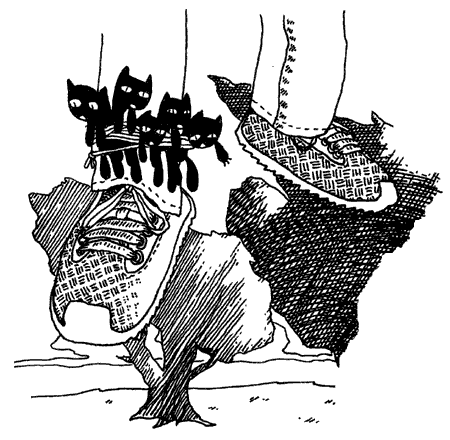
\includegraphics[width=0.5625\textwidth]{cache/41.png}}

Forthwith there is a rustling in the trees behind Paij-ree's house and
it turns out to be a man falling from the sky.  His name is Doug and
he sells cats.

So, just as he comes into to view, when his shadow (and the shadows of
the cats tied to his foot) obscures the bird on the lawn that we're
trying to hit with a racquetball, as he's squeezing a wisp of helium
from his big balloon, we shout, ``Hello, Doug!''

And he says, ``Hello, Gonk-ree!  Hello, Why!''

Paij-ree checks his pockets to be sure he has the dollar-twenty-seven
he'll need in order to buy the three cats he'll need to keep the
furnace stoked and the satellite dish turning.  These cats generate
gobs of static once Paij-ree tosses them in the generator, where
they'll be outnumbered by the giant glass rods, which caress the cats
continually-- But, wait!  Did you see how the cat broker called him
Gonk-ree?

And he calls him Gonk-ree in the morning and Gonk-plo at night.

So the suffix is definitely subject to the sunlight.  As far as I can
tell, the prefix indicates the namecaller's relationship to Paij-ree.


\begin{lstlisting}[basicstyle=\ttfamily\color{basiccolor},
    commentstyle = \ttfamily\color{commentcolor},
    keywordstyle=\ttfamily\color{keywordscolor},
    stringstyle=\color{stringcolor},
    language=Ruby,
    basicstyle=\small\ttfamily,
    showstringspaces=false,
  ]

 class String

   # The parts of my daughter's organ
   # instructor's name.
   @@syllables = [
     { 'Paij' => 'Personal',
       'Gonk' => 'Business',
       'Blon' => 'Slave',
       'Stro' => 'Master',
       'Wert' => 'Father',
       'Onnn' => 'Mother' },
     { 'ree'  => 'AM',
       'plo'  => 'PM' }
   ]

   # A method to determine what a
   # certain name of his means.
   def name_significance
     parts = self.split( '-' )
     syllables = @@syllables.dup
     signif = parts.collect do |p|
       syllables.shift[p]
     end
     signif.join( ' ' )
   end

 end

\end{lstlisting}


Now I've gone beyond just showing you sloppy code.  Here be a grave
debauchery and a crime against nature.  A crime most languages won't
allow you to commit.  We're changing the
\lstinline[breaklines=true]|String|, {\bf one of the core classes of
  Ruby}!

``I know this is a bit dangerous,'' I said, when I passed this one
under Paij-ree's nose. ``I hope nobody gets hurt.''

``Every Smotchkkiss must taste what this (kep-yo-iko) danger does,''
he said.  ``Dogs and logs and swampy bogs (kul-ip), all must be
tasted.''  And he took a swig of his Beagle Berry marsh drink.

So what is it that I'm adding to the
\lstinline[breaklines=true]|String| class?  Two things: a class
variable and a method.  A normal {\bf instance method}.

I like to look at the {\bf at} symbol as a character meaning {\bf
  attribute}.  The {\bf double at} stands for {\bf attribute all}.  A
class variable.  All instances of a class can look at this variable
and it is the same for all of them.  The
\lstinline[breaklines=true]|@@syllables| variable is an Array that can
now be used inside the String class.

The new method is \lstinline[breaklines=true]|name_significance| and
this new method can be used with any string.

\begin{quote}
\lstinline[breaklines=true]|print "Paij-ree".name_significance| prints
out \lstinline[breaklines=true]|Personal AM|.\end{quote}


As you can see, Paij-ree is a personal name.  A name friends use in
the early hours.

Make sure you see the line of code which uses
\lstinline[breaklines=true]|self|.  This is a special variable, a
variable which represents the object whose method you are calling.  To
simplify things a bit, let's try making a method which breaks up a
string on its dashes.


\begin{lstlisting}[basicstyle=\ttfamily\color{basiccolor},
    commentstyle = \ttfamily\color{commentcolor},
    keywordstyle=\ttfamily\color{keywordscolor},
    stringstyle=\color{stringcolor},
    language=Ruby,
    basicstyle=\small\ttfamily,
    showstringspaces=false,
  ]

 class String
   def dash_split
     self.split( '-' )
   end
 end

\end{lstlisting}


Again, here's a method which can be used with any string.

\begin{quote}
\lstinline[breaklines=true]|"Gonk-plo".dash_split| return the Array
\lstinline[breaklines=true]|['Gonk', 'plo']|.\end{quote}


Using \lstinline[breaklines=true]|self| marks the beginning of
crossing over into many of the more advanced ideas in Ruby. This is
definition language.  You're defining a method, designing it before it
gets used.  You're preparing for the existence of an object which uses
that method.  You're saying, ``When
\lstinline[breaklines=true]|dash_split| gets used, there will be a
string at that time which is the one we're dash-splitting.  And
\lstinline[breaklines=true]|self| is a special variable which refers
to that string.''

Ruby is a knockout definition language.  A succulent and
brain-splitting discussion is coming your way deeper in this book.

Most often you won't need to use \lstinline[breaklines=true]|self|
explicitly, since you can call methods directly from inside other
method definitions.


\begin{lstlisting}[basicstyle=\ttfamily\color{basiccolor},
    commentstyle = \ttfamily\color{commentcolor},
    keywordstyle=\ttfamily\color{keywordscolor},
    stringstyle=\color{stringcolor},
    language=Ruby,
    basicstyle=\small\ttfamily,
    showstringspaces=false,
  ]

 class String
   def dash_split; split( '-' ); end
 end

\end{lstlisting}


In the \lstinline[breaklines=true]|name_significance| method, find the
loop.  Learning about \lstinline[breaklines=true]|Array#collect| is
essential. Let's look close.


\begin{lstlisting}[basicstyle=\ttfamily\color{basiccolor},
    commentstyle = \ttfamily\color{commentcolor},
    keywordstyle=\ttfamily\color{keywordscolor},
    stringstyle=\color{stringcolor},
    language=Ruby,
    basicstyle=\small\ttfamily,
    showstringspaces=false,
  ]

 signif = parts.collect do |p|
   syllables.shift[p]
 end

\end{lstlisting}


The \lstinline[breaklines=true]|parts| Array contains the separated
name.  \lstinline[breaklines=true]|['Paij', 'plo']|, for instance.
We're iterating through each item in that Array with
\lstinline[breaklines=true]|collect|.  But
\lstinline[breaklines=true]|collect| steps beyond what
\lstinline[breaklines=true]|each| does.  Like
\lstinline[breaklines=true]|each|, collect slides each item down the
chute as a block variable.  And then, at the end of the block,
\lstinline[breaklines=true]|collect| {\bf keeps the answer the block
  gives back and adds it to a new Array}.  The
\lstinline[breaklines=true]|collect| method is the perfect way of
building a new Array which is based on the items in an existing Array.

Doug has three cats for sale.  One is twelve cents, one is sixty-three
cents, one is nine cents. Let's see how much each cat would cost if we
added a 20% tip.


\begin{lstlisting}[basicstyle=\ttfamily\color{basiccolor},
    commentstyle = \ttfamily\color{commentcolor},
    keywordstyle=\ttfamily\color{keywordscolor},
    stringstyle=\color{stringcolor},
    language=Ruby,
    basicstyle=\small\ttfamily,
    showstringspaces=false,
  ]

 catsandtips = [0.12, 0.63, 0.09].collect { |catcost| catcost + ( catcost * 0.20 ) }

\end{lstlisting}


I say Paij-ree's property is a very charming section of woods when
it's not raining cats and Doug. For many days, Paij-ree and I camped
in tents by the river behind his house, subsisting on smoked blackbird
and whittling little sleeping indians by the dusklight.  On occassion
he would lose a game of spades and I knew his mind was distracted,
thinking of Endertromb.  All of this must have been stirring inside of
him for sometime.  I was the first ear he'd ever had.

``I just came from Ambrose,'' I said.  ``Sort of my own underground
home, a place where elves strive to perfect animals.''

He mumbled and nodded.  ``You can't be (poth-in-oin) part of (in) such
things.''

``You think we will fail?''

``I (preep) have been there before,'' he said.  And then, he spoke of
the Lotteries.

\newpage


\section{The Goat Wants to Watch a Whole Film}



	\includegraphics[width=1.0\textwidth]{cache/42.png}

The elevator had opened into a green room full of shelves and file
cabinets.  Reels of tape and film canisters and video tape everywhere.
Dr. Cham hadn't a clue what most of it was.  All he saw was a big,
futuristic mess.

He called out again, stumbling through alleys of narrow shelves,
``Hello-o-o??  I'm looking for intellegent life!  I'm a space
traveller!''  He tripped when his foot slid right into a VCR
slot. ``Any other beings I can communicate with?''

Hand cupped around mouth, he yelled, ``Hello-o-o?''

``Crying out loud.''  The sleepy goat came tromping down the aisle.

\newpage


	\includegraphics[width=1.0\textwidth]{cache/43.png}

``I hate that book,'' said the goat.  ``I believe the author is
        disingenuous.''

``Really?'' asked Dr. Cham.

``I'm sure it's all true.  It's just so heavily embellished.  I'm
        like: Enough already.  I get it.  Cut it out.''

``I'm not quite sure what to make of it,'' said the Doctor.  ``It
        seems like an honest effort. I actually wrote something in
        Ruby back there.''

``It doesn't give goats a very good name,'' said the goat.

``But you are the only goat in the book,'' said the Doctor.

``And I'm totally misquoted.''

	\includegraphics[width=1.0\textwidth]{cache/44.png}

The goat closed his mouth and Dr. Cham held his heart.

``I'm actually very literate,'' said the goat.  ``Albeit, more
recently, I've switched to movies.  I love foreign films.  One of my
relatives just brough back {\em Ishtar} from your planet.  Wow, that
was excellent.''  ``I haven't been to my planet in a long time.  It
would be difficult to consider it my home at this stage.''

``Well, Warren Beatty is delightful.  His character is basically
socially crippled.  He actually tries to kill himself, but Dustin
Hoffman sits in the window sill and starts crying and singing this
totally hilarious heartbreak song.  I've got it here, you should see
it.''

	\begin{sidebar}{}{20}
\begin{verbatim}
		we want a tambourine!
           /
          |  we want all a tambourine!
          |      /
          \__  |
        /  o o \__/\__/\_
      /.           \ o o \____
       /'      ----/          \
_____ /  '    / /.\\   #------/
       /     /        /     \\
             /       ///
      /so               \
           /\   \me time\\..
       /pp/  \s these pictur\\
      /es/   \don't w\ \ork out\
     ***      *** right but i
       think this time
          they did
            ooo o
             oo
            o
         o
      {o}
   ^
\end{verbatim}
	\end{sidebar}

``Can I get something to eat?'' asked the Doctor.  And he still felt
filthy.

``How about we watch a film and you can have a buttermelon with
tentacles?'' said the goat.

So, they worked their way back toward the goat's projector.  Back by
the freezer locker, they sat on a giant rug and broke off the
appendages of frozen buttermelons.  The shell was solid, but once it
cracked, rich fruit cream was in abundance.  Sweet to taste and a very
pleasant scent.

``First film, you've got to see,'' said the goat.  ``Locally filmed
and produced.  I'm good friends with the lady who did casting.  Dated
her for awhile.  Knew everyone who was going to play the different
roles long before it was announced.''

The goat set the projector by Dr. Cham.  ``I've got the music on the
surround sound. You can man the knob.''

	\includegraphics[width=1.0\textwidth]{cache/45.png}

Dr. Cham's mind wandered at this point in the presentation, just as
the land war mounted between the two throngs of animal settlers.  The
details of their wars and campaigns continued to consume the spool of
transparent film that Dr. Cham was feeding through the projector.

War after war after war.  The Sieging of Elmer Lake.  The Last Stand
of Newton P. Giraffe and Sons.  Dog Invasion of Little Abandoned
Cloud.  No animals died in these wars.  Most often an attack consisted
of bopping another animal on the head.  And they philipped each
other's noses.  But, believe me, it was humiliating.

Blasted crying shame.  Things could have worked out.



\subsection{The Birth of an Object}



``Don't worry,'' said the goat, anxious to sway Dr. Cham's attention
back to the film.  ``Things {\em do} work out.''

In Ruby, the Object is the very center of all things.  It is The
Original.


\begin{lstlisting}[basicstyle=\ttfamily\color{basiccolor},
    commentstyle = \ttfamily\color{commentcolor},
    keywordstyle=\ttfamily\color{keywordscolor},
    stringstyle=\color{stringcolor},
    language=Ruby,
    basicstyle=\small\ttfamily,
    showstringspaces=false,
  ]

 class ToastyBear < Object; end

\end{lstlisting}


The angle bracket indicates {\bf inheritance}.  This means that the
new \lstinline[breaklines=true]|ToastyBear| class is a new class based
on the \lstinline[breaklines=true]|Object| class.  Every method that
\lstinline[breaklines=true]|Object| has will be available in
\lstinline[breaklines=true]|ToastyBear|.  Constants available in
\lstinline[breaklines=true]|Object| will be available in
\lstinline[breaklines=true]|ToastyBear|.

But every object inherits from \lstinline[breaklines=true]|Object|.
The code...


\begin{lstlisting}[basicstyle=\ttfamily\color{basiccolor},
    commentstyle = \ttfamily\color{commentcolor},
    keywordstyle=\ttfamily\color{keywordscolor},
    stringstyle=\color{stringcolor},
    language=Ruby,
    basicstyle=\small\ttfamily,
    showstringspaces=false,
  ]

 class ToastyBear; end

\end{lstlisting}


Is identical to...


\begin{lstlisting}[basicstyle=\ttfamily\color{basiccolor},
    commentstyle = \ttfamily\color{commentcolor},
    keywordstyle=\ttfamily\color{keywordscolor},
    stringstyle=\color{stringcolor},
    language=Ruby,
    basicstyle=\small\ttfamily,
    showstringspaces=false,
  ]

 class ToastyBear < Object; end

\end{lstlisting}


Inheritance is handy.  You can create species of objects which relate
to each other. Often, when you're dissecting a problem, you'll come
across various objects which share attributes.  You can save yourself
work by inheriting from classes which already solve part of that
problem.

You may have a \lstinline[breaklines=true]|UnitedStatesAddress| class
which stores the address, city, state, and zip code for someone living
in the United States.  When you start storing addresses from England,
you could add a \lstinline[breaklines=true]|UnitedKingdomAddress|
class.  If you then ensure that both addresses inherit from a parent
\lstinline[breaklines=true]|Address| class, you can design your
mailing software to accept any kind of address.


\begin{lstlisting}[basicstyle=\ttfamily\color{basiccolor},
    commentstyle = \ttfamily\color{commentcolor},
    keywordstyle=\ttfamily\color{keywordscolor},
    stringstyle=\color{stringcolor},
    language=Ruby,
    basicstyle=\small\ttfamily,
    showstringspaces=false,
  ]

 def mail_them_a_kit( address )
   unless address.is_a? Address
     raise ArgumentError, "No Address object found."
   end
   print address.formatted
 end

\end{lstlisting}


Also, inheritance is great if you want to override certain behaviours
in a class. For example, perhaps you want to make your own slight
variation to the \lstinline[breaklines=true]|Array| class. You want to
enhance the \lstinline[breaklines=true]|join| method.  But if you
change \lstinline[breaklines=true]|Array#join| directly, you will
affect other classes in Ruby that use Arrays.

So you start your own class called
\lstinline[breaklines=true]|ArrayMine|, which is based on The Original
\lstinline[breaklines=true]|Array|.


\begin{lstlisting}[basicstyle=\ttfamily\color{basiccolor},
    commentstyle = \ttfamily\color{commentcolor},
    keywordstyle=\ttfamily\color{keywordscolor},
    stringstyle=\color{stringcolor},
    language=Ruby,
    basicstyle=\small\ttfamily,
    showstringspaces=false,
  ]

 class ArrayMine < Array
   # Build a string from this array, formatting each entry
   # then joining them together.
   def join( sep = $,, format = "%s" )
     collect do |item|
       sprintf( format, item )
     end.join( sep )
   end
 end

\end{lstlisting}


\lstinline[breaklines=true]|ArrayMine| is now a custom
\lstinline[breaklines=true]|Array| class with its own
\lstinline[breaklines=true]|join| method.
\lstinline[breaklines=true]|Array| is the {\bf superclass} of
\lstinline[breaklines=true]|ArrayMine|.  Every object has a
\lstinline[breaklines=true]|superclass| method where you can verify
this relationship.


\begin{lstlisting}

 irb> ArrayMine.superclass
   => Array

\end{lstlisting}


Perfect.  We manage a hotel and we have an
\lstinline[breaklines=true]|Array| of our room sizes:
\lstinline[breaklines=true]|[3, 4, 6]|. Let's get it nicely printed
for a brochure.


\begin{lstlisting}[basicstyle=\ttfamily\color{basiccolor},
    commentstyle = \ttfamily\color{commentcolor},
    keywordstyle=\ttfamily\color{keywordscolor},
    stringstyle=\color{stringcolor},
    language=Ruby,
    basicstyle=\small\ttfamily,
    showstringspaces=false,
  ]

 rooms = ArrayMine[3, 4, 6]
 print "We have " + rooms.join( ", ", "%d bed" ) + " rooms available."

\end{lstlisting}


Which prints, ``We have 3 bed, 4 bed, 6 bed rooms available.''

Dr. Cham was looking around for a bathroom, but archival video tape
was everywhere. He eventually found a place, it may have been a
bathroom.  It had a metal bin. More importantly, it was dark and out
of eyesight.

While he's in there, let me add that while The Originals slaughtered
The Invaders to prove their rights as First Creatures, the Ruby Object
doesn't have any such dispute.  It is the absolute king Object the
First.

Watch.


\begin{lstlisting}

 irb> Class.superclass
   => Module
 irb> Kernel.class
   => Module
 irb> Module.superclass
   => Object
 irb> Object.superclass
   => nil

\end{lstlisting}


Even \lstinline[breaklines=true]|Class| is an
\lstinline[breaklines=true]|Object|!  See, although classes are the
definition language for objects, we still call class methods on them
and treat them like objects occassionally.  It may seem like a
dizzying circle, but it's truly a very strict parentage.  And it
ensures that when you alter the \lstinline[breaklines=true]|Object|,
you alter {\bf everything in Ruby}.  Which is impossibly scary and
all-powerful and cataclysmic and awesome!  {\bf Ruby does not restrict
  you, my sister, my brother!}

Between \lstinline[breaklines=true]|Class| and
\lstinline[breaklines=true]|Object|, do you see
\lstinline[breaklines=true]|Module|?  If
\lstinline[breaklines=true]|Object| is the king, the one who has sired
every other part of Ruby, then \lstinline[breaklines=true]|Module| is
the poor waifish nun, shielding and protecting all her little Ruby
townspeople children.  (To complete the analogy:
\lstinline[breaklines=true]|Class| is the village school teacher and
\lstinline[breaklines=true]|Kernel| is the self-important colonel.)

The whole point of \lstinline[breaklines=true]|Module|'s existence is
to give food and shelter to code.  Methods can stay dry under
\lstinline[breaklines=true]|Module|'s shawl.
\lstinline[breaklines=true]|Module| can hold classes and constants and
variables of any kind.

``But what does a Module {\em do}?'' you ask.  ``How is it gainfully
employed??''

``That's all it does!!'' I retort, stretching out my open palms in the
greatest expression of futility known to man.  ``Now hear me -- for I
will never speak it again -- that Module Mother Superior has given
these wretched objects a place to stay!!''


\begin{lstlisting}[basicstyle=\ttfamily\color{basiccolor},
    commentstyle = \ttfamily\color{commentcolor},
    keywordstyle=\ttfamily\color{keywordscolor},
    stringstyle=\color{stringcolor},
    language=Ruby,
    basicstyle=\small\ttfamily,
    showstringspaces=false,
  ]

 # See, here is the module -- where else could our code possibly stay?
 module WatchfulSaintAgnes

   # A CONSTANT is laying here by the doorway.  Fine.
   TOOTHLESS_MAN_WITH_FORK = ['man', 'fork', 'exposed gums']

   # A Class is eating, living well in the kitchen.
   class FatWaxyChild; end

   # A Method is hiding back in the banana closet, God knows why.
   def timid_foxfaced_girl; {'please' => 'i want an acorn please'}; end

 end

\end{lstlisting}


Now you have to go through Saint Agnes to find them.


\begin{lstlisting}

 >> WatchfulSaintAgnes::TOOTHLESS_MAN_WITH_FORK
 => ["man", "fork", "exposed gums"]
 >> WatchfulSaintAgnes::FatWaxyChild.new
 => #<WatchfulSaintAgnes::FatWaxyChild:0xb7d2ad78>
 >> WatchfulSaintAgnes::instance_methods
 => ["timid_foxfaced_girl"]

\end{lstlisting}


Always remember that a \lstinline[breaklines=true]|Module| is only an
inn.  A roof over their heads.  It is not a self-aware
\lstinline[breaklines=true]|Class| and, therefore, cannot be brought
to life with \lstinline[breaklines=true]|new|.


\begin{lstlisting}

 >> WatchfulSaintAgnes.new
 NoMethodError: undefined method `new' for WatchfulSaintAgnes:Module
         from (irb):2

\end{lstlisting}


St. Agnes has given up her whole life in order that she may care for
these desperate bits of code. Please.  Don't take that away from her.

If you wanted to steal from St. Agnes, though, I can help you. You can
bring in a larger abbey to swallow up the ministry of
\lstinline[breaklines=true]|WatchfulSaintAgnes| and then what is she
left with?

For this you can use \lstinline[breaklines=true]|extend|, which will
pull all the methods from a module into a class or an object.


\begin{lstlisting}

 >> class TheTimeWarnerAolCitibankCaringAndLovingFacility; end
 >> TheTimeWarnerAolCitibankCaringAndLovingFacility.extend WatchfulSaintAgnes
 >> TheTimeWarnerAolCitibankCaringAndLovingFacility::instance_methods
 => ["timid_foxfaced_girl"]

\end{lstlisting}


In truth, no one's {\em stolen} from
\lstinline[breaklines=true]|WatchfulSaintAgnes|, only borrowed.  The
\lstinline[breaklines=true]|timid_foxfaced_girl| now has two
addresses.

You gotta admit.  The old abbey can get bought out a zillion times and
that little fox-faced girl will {\em still} be back in the banana
closet wanting an acorn!  Too bad we can't feed her. She's a method
with no arguments.

When Dr. Cham came out refreshed, the filmstrip was a bit behind.  But
the goat hadn't noticed, so the Doctor advanced frames until it made
some sense.

\newpage

	\includegraphics[width=1.0\textwidth]{cache/46.png}

So the invaders left the planet.

``This planet {\em is} decrepit,'' said Dr. Cham.  ``The castle is
nice.  But inside it's a disaster.''

``The whole castle look is a projection,'' said the goat.  ``All the
flowers and apple blossoms and the sky even.  It's a low-resolution
projection.''

``Yes?  It is enchanting.''

``I guess.''

	\includegraphics[width=1.0\textwidth]{cache/47.png}

``That's messed up!'' said the goat.  ``That's not the way the film
        ends! There's no blood!  What happened?  What happened?  Did
        you screw up the knob, idiot?''

``Well, I don't know,'' said Dr. Cham.  He turned the knob reverse and
        forward. Tapped the lens.

``Check the film!  Check the film!''

Dr. Cham pulled out a length of film from the projection feed, melted
and dripping from its end.

``Curse that!  These projectors are quality!  I've never had this
happen.  There's no way.''



\subsection{Hunting For a Voice}



``I don't think it was the projector,'' said Dr. Cham.  ``Something
flew across that screen and uttered a blistering moan.''

``I don't have any dupes of that movie,'' said the goat somberly.
``And that girl.  That casting director.  I never see her anymore.''

Dr. Cham stood up and looked over the dumpy aisles of magnetic
carnage, searching.

``Oh, hey, you should call that girl,'' the goat went on. ``You could
talk to her, get an understanding. Tell her about me.  Don't act like
your my friend, just, you know, `Oh, that guy? Yeah, whatta maroon.'''

Dr. Cham spotted the doorway and exited.

The hallways were an entirely new world of mess.  In the goat's
archives, the shelves had been messy. In the hallway, shelves were
completely tipped.  Sinks were falling through the ceiling.  The
Doctor ventured under the debris, kicking through plywood when
necessary.

``You shouldn't be out here,'' said the goat.  ``You're on someone
else's property at this point. A couple of pygmy elephants own all
this.  They're nasty guys.  They'll beat the crap outta you with their
trunks.  They ball it up and just whack ya.''

Dr. Cham pushed a file cabinet out of his way, which fell through a
flimsy wall, then through the floor of the next room over.  And they
heard it fall through several floors after that.

``I'm trying to remember how it goes in the book,'' said Dr. Cham, as
he walked swiftly through the hall.  ``That milky fog that swept
across the projection.  We find that thing.''  He jiggled a door
handle, broke it off.  Forged through the doorway and disappeared
inside.

``You really get a kick out of beating stuff up, don't you?'' said the
goat.  ``Walls, doors.'' The goat headbutted a wall.  The wall
shuddered and then laid still.

Then, it was quiet.  And black.

The goat stayed put in the bleak hallway, expecting Dr. Cham to flip
over a few desks and emerge, ready to move on from the room he'd
busted into.  But Dr. Cham didn't return, and the goat opted to share
a moment with the neglected wreckage left by his neighbors.  Not that
he could see at all. He could only hear the occassional rustling of
the piles of invoices and carbon copy masters and manila envelopes
when he shifted his legs.

The ground seemed to buckling right under the goat, as if the heaps of
kipple around him were beginning to slide toward his weight.  He would
be at the center of this whirlpool of elephant documentation.  Would
he die of papercuts first?  Or would he suffocate under the solid
burial by office supplies?

A soft light, however, crept up to him.  A floating, silver fish.  No,
it was a -- was it scissors? The scissors grew into a shimmering
cluster of intellegent bread, each slice choking on glitter. But, no,
it was hands.  And an Easter hat.

	\includegraphics[width=1.0\textwidth]{cache/48.png}

In another room, Dr. Cham stood under the clear glass silently.  The
ceiling had abruptly gone transparent, then starlight washed over his
pants and jacket.  He walked further to the room's center in muted
colors, lit as softly as an ancient manuscript in its own box at the
museum.  More stars, more cotton clusters of fire, unveiled as he came
across the floor. And it peeked into view soon enough, he expected it
to be larger, but it wasn't.

Earth.  Like a painted egg, still fresh.  He felt long cello strings
sing right up against his spine.  How could that be called Peoplemud?
Here was a vibrant and grassy lightbulb.  The one big ball that had
something going for it.

He thought of The Rockettes.  Actually, he missed The Rockettes.  What
a bunch of great dancers.  He had yelled something to The Rockettes
when he saw them.  Something very observant and flattering.

Oh, yes, while The Rockettes were spinning, arm in arm, he had yelled,
``Concentric circles!'' Which no one else cared to observe.

And this thought was enough to feed Dr. Cham's superiority complex.
He wore a goofy smile as he retraced his footsteps.  He truthfully
felt his genius coming through in such a statement.  To realize the
simplicity of a circle was his.  He reflected on it all the way back
to the hallway.

Which I think is great.  Adore yourself when you have a second.

	\includegraphics[width=1.0\textwidth]{cache/49.png}

``Oh, right,'' said the goat.  ``Your niece.  The niece you killed.
        I'm with ya now.''

For just a few moments, they all looked at each other.  Just enough
time for both Dr. Cham and the goat to think: {\em Oh, yeah.  Hannah
  causes us a lot of trouble.  She's already talking about maple
  donuts.}

``Does she start talking about maple donuts right away like that?''
asked the goat.

``Yes, she does,'' said the Doctor.  ``She brings it up to you, then
she brings it up to me.  She sees a maple donut somewhere -- I don't
quite remember where.''

``Do I see a real maple donut?'' Hannah said.  ``I need a real one.''

``Okay, okay,'' said the goat.  ``Yeah, I remember: here's where she
says that if she gets a real maple donut, she'll become a real person
again. Because her real destiny was to own a bakery and you ruined
that destiny and now she's trapped as a ghost.''

``Hey, that's the truth!'' Hannah yelped.

``It's terrible that we must bear through this whole scene again,''
said the Doctor.  ``The donuts are immaterial.  They should be left
out altogether.''

``Man, I am having a {\em hard} time remembering all of this
chapter,'' said the goat.  ``I don't even remember how to get out of
this hallway.  I must have read that book like thirty times.  Do we
blast through a wall?  Do we scream until someone finds us?''

``We get Hannah to float through walls and she finds some kind of
machine,'' says Dr. Cham.  ``I have to write a program -- it all works
out somehow.''

``But, you know what I'm saying?'' said the goat.  ``I forget all the
details. Especially the earlier chapters.  I mean I can remember the
ending perfectly. It's hard to sit through all this.  The end is so
much better.''

Dr. Cham folded his arms and teetered on a heel.  ``The porcupine.''
He smiled greedily at the goat.

``Oh, totally.  The porcupine is definitely who I want to meet,'' said
the goat.  ``I wonder what he does with all that money when the book
is over.''

Dr. Cham nodded respectfully.  ``I'm very excited to see him wearing
slippers.''

``Those infernal slippers!'' said the goat and he haw-hawed coarsely,
a shower of saliva cascading from his jaws.

Hannah's mind rattled, waiting for this nonsense to break for a
moment. She tipped her head on its side and the rattle slid along the
curve of her cranium.  The little noise died away, though, as the back
of her head vanished ({\em fluxed out} is what she called it) and then
her head was back again with its little rattle and she caught herself
doing that careless moaning again.  {\bf HRRRRRR-RRR-OH-RRRR-RRRR.}

``I'm not as into the chunky bacon stuff,'' said the goat.  ``I don't
see what's so great about it.''

Could she speak while moaning? {\bf BON-BON.}  With a French moan.
{\bf BOHN-BOHN. BOHN-APPE-TEET-OHHHH-RRRR.}

``I know she's harmless, but that sound freaks me out.  My hair is
{\bf completely} on end.''

``Hannah?'' said Dr. Cham.  ``Where are you, child?  Come do a good
turn for us, my niece.''

She was right near them, in and out.  And they could hear her cleaning
up her voice, bright, speaking like a angel scattering stardust. Yes,
the whole maple donut story came out again, and more about the bakery
she would own, the muffins and rolls and baguettes.

\newpage


\section{The Theft of the Lottery Captain}



	\parpic[r]{\includegraphics[width=0.2875\textwidth]{cache/50.png}}

And now, Paij-ree's stories of the Lotteries.

On Endertromb, the organist's father invented the lottery.  The idea
came while he was praying to Digger Dosh.

Digger Dosh is sort of like their God.  But ten times scarier.  This
guy dug an infinitely deep tunnel straight through the planet and came
out dead. But he's really not dead.  He's really just {\em one second}
behind them.  And he eats time.

It's kind of complicated because Digger Dosh totally kills people.
But I guess if you do what he says, it's not so bad.  Maybe I'll talk
about it later.  It's such a pain to talk about because it's so scary
and yet one of my friends actually believes the whole thing.  I get
kind of choked up -- not like I'm crying, more like I'm choking.

Anyway, once while praying, three numbers came to Paij-ree's father.

He then asked his mind, ``What are these numbers?''

And his mind played a short video clip of him selling all kinds of
numbers.  And, for years and years, travelling and selling numbers.

And he asked his brain, ``People will buy numbers?''

And his brain said, ``If they buy the right three numbers, give them a
prize.''

At which he imagined himself launching off a ski jump and showering
people with presents.  No question: he would be an icon.

So he went and did as his brain said and sold numbers.  The father's
simple lottery consisted of three unique numbers, drawn from a set of
25 numbers.


\begin{lstlisting}[basicstyle=\ttfamily\color{basiccolor},
    commentstyle = \ttfamily\color{commentcolor},
    keywordstyle=\ttfamily\color{keywordscolor},
    stringstyle=\color{stringcolor},
    language=Ruby,
    basicstyle=\small\ttfamily,
    showstringspaces=false,
  ]

 class LotteryTicket

   NUMERIC_RANGE = 1..25

   attr_reader :picks, :purchased

   def initialize( *picks )
     if picks.length != 3
       raise ArgumentError, "three numbers must be picked"
     elsif picks.uniq.length != 3
       raise ArgumentError, "the three picks must be different numbers"
     elsif picks.detect { |p| not NUMERIC_RANGE === p }
       raise ArgumentError, "the three picks must be numbers between 1 and 25."
     end
     @picks = picks
     @purchased = Time.now
   end

 end

\end{lstlisting}


Yes, the \lstinline[breaklines=true]|LotteryTicket| class contained
the three numbers (\lstinline[breaklines=true]|@picks|) and the time
when the ticket was bought (\lstinline[breaklines=true]|@purchased|).
The allowed range of numbers (from {\bf one} to {\bf twenty-five}) is
kept in the constant \lstinline[breaklines=true]|NUMERIC_RANGE|.

The \lstinline[breaklines=true]|initialize| method here can have any
number of arguments passed in.  The {\bf asterisk} in the
\lstinline[breaklines=true]|picks| argument means that {\bf any
  arguments will be passed in as an Array}.  Having the arguments in
an Array means that methods like \lstinline[breaklines=true]|uniq| and
\lstinline[breaklines=true]|detect| can be used on the arguments
together.

This class contains two definitions: the method definition
(\lstinline[breaklines=true]|def|) and an attributes definition
(\lstinline[breaklines=true]|attr_reader|).  Both are {\bf really just
  method definitions} though.

The \lstinline[breaklines=true]|attr_reader| shortcut is identical to
writing this Ruby code:


\begin{lstlisting}[basicstyle=\ttfamily\color{basiccolor},
    commentstyle = \ttfamily\color{commentcolor},
    keywordstyle=\ttfamily\color{keywordscolor},
    stringstyle=\color{stringcolor},
    language=Ruby,
    basicstyle=\small\ttfamily,
    showstringspaces=false,
  ]

 class LotteryTicket
   def picks; @picks; end
   def purchased; @purchased; end
 end

\end{lstlisting}


Attributes are wrapper methods for instance variables (such as
\lstinline[breaklines=true]|@picks|) which can be used {\bf outside of
  the class itself}.  Paij-ree's father wanted to code a machine which
could read the numbers and the date of purchase from the ticket.  In
order to do that, those instance variables must be exposed.

Let's create a random ticket and read back the numbers:


\begin{lstlisting}[basicstyle=\ttfamily\color{basiccolor},
    commentstyle = \ttfamily\color{commentcolor},
    keywordstyle=\ttfamily\color{keywordscolor},
    stringstyle=\color{stringcolor},
    language=Ruby,
    basicstyle=\small\ttfamily,
    showstringspaces=false,
  ]

 ticket = LotteryTicket.new( rand( 25 ) + 1,
             rand( 25 ) + 1, rand( 25 ) + 1 )
 p ticket.picks

\end{lstlisting}


Running the above, I just got: 
\lstinline[breaklines=true]|[23, 14, 20]|.  
You will get an error if two of the random numbers happen to
be identical.

However, I can't change the lottery ticket's picks from outside of the
class.


\begin{lstlisting}[basicstyle=\ttfamily\color{basiccolor},
    commentstyle = \ttfamily\color{commentcolor},
    keywordstyle=\ttfamily\color{keywordscolor},
    stringstyle=\color{stringcolor},
    language=Ruby,
    basicstyle=\small\ttfamily,
    showstringspaces=false,
  ]

 ticket.picks = [2, 6, 19]

\end{lstlisting}


I get an error: 
\lstinline[breaklines=true]|undefined method `picks='|. 
This is because \lstinline[breaklines=true]|attr_reader|
only adds a {\bf reader} method, not a writer method. That's fine,
though.  We don't want the numbers or the date to change.

So, the tickets are {\em objects}.  Instances of the
\lstinline[breaklines=true]|LotteryTicket| class.  Make a ticket with
\lstinline[breaklines=true]|LotteryTicket.new|.  Each ticket has it's
own \lstinline[breaklines=true]|@picks| and it's own
\lstinline[breaklines=true]|@purchased| instance variables.

The lottery captain would need to draw three random numbers at the
close of the lottery, so we'll add a convenient class method for
generating random tickets.


\begin{lstlisting}[basicstyle=\ttfamily\color{basiccolor},
    commentstyle = \ttfamily\color{commentcolor},
    keywordstyle=\ttfamily\color{keywordscolor},
    stringstyle=\color{stringcolor},
    language=Ruby,
    basicstyle=\small\ttfamily,
    showstringspaces=false,
  ]

 class LotteryTicket
   def self.new_random
     new( rand( 25 ) + 1, rand( 25 ) + 1, rand( 25 ) + 1 )
   end
 end

\end{lstlisting}


Oh, no.  But we have that stupid error that pops up if two of the
random numbers happen to be identical.  If two numbers are the same,
the \lstinline[breaklines=true]|initialize| throws an
\lstinline[breaklines=true]|ArgumentError|.

The trick is going to be restarting the method if an error happens. We
can use Ruby's \lstinline[breaklines=true]|rescue| to handle the error
and \lstinline[breaklines=true]|redo| to start the method over.


\begin{lstlisting}[basicstyle=\ttfamily\color{basiccolor},
    commentstyle = \ttfamily\color{commentcolor},
    keywordstyle=\ttfamily\color{keywordscolor},
    stringstyle=\color{stringcolor},
    language=Ruby,
    basicstyle=\small\ttfamily,
    showstringspaces=false,
  ]

 class LotteryTicket
   def self.new_random
     new( rand( 25 ) + 1, rand( 25 ) + 1, rand( 25 ) + 1 )
   rescue ArgumentError
     redo
   end
 end

\end{lstlisting}


Better.  It may take a couple times for the numbers to fall together
right, but it'll happen.  The wait will build suspense, huh?

The lottery captain kept a roster of everyone who bought tickets,
along with the numbers they drew.


\begin{lstlisting}[basicstyle=\ttfamily\color{basiccolor},
    commentstyle = \ttfamily\color{commentcolor},
    keywordstyle=\ttfamily\color{keywordscolor},
    stringstyle=\color{stringcolor},
    language=Ruby,
    basicstyle=\small\ttfamily,
    showstringspaces=false,
  ]

 class LotteryDraw
   @@tickets = {}
   def LotteryDraw.buy( customer, *tickets )
     unless @@tickets.has_key?( customer )
       @@tickets[customer] = []
     end
     @@tickets[customer] += tickets
   end
 end

\end{lstlisting}


Yal-dal-rip-sip was the first customer.


\begin{lstlisting}[basicstyle=\ttfamily\color{basiccolor},
    commentstyle = \ttfamily\color{commentcolor},
    keywordstyle=\ttfamily\color{keywordscolor},
    stringstyle=\color{stringcolor},
    language=Ruby,
    basicstyle=\small\ttfamily,
    showstringspaces=false,
  ]

 LotteryDraw.buy 'Yal-dal-rip-sip',
     LotteryTicket.new( 12, 6, 19 ),
     LotteryTicket.new( 5, 1, 3 ),
     LotteryTicket.new( 24, 6, 8 )

\end{lstlisting}


When it came time for the lottery draw, Paij-ree's father (the lottery
captain) added a bit of code to randomly select the numbers.


\begin{lstlisting}[basicstyle=\ttfamily\color{basiccolor},
    commentstyle = \ttfamily\color{commentcolor},
    keywordstyle=\ttfamily\color{keywordscolor},
    stringstyle=\color{stringcolor},
    language=Ruby,
    basicstyle=\small\ttfamily,
    showstringspaces=false,
  ]

 class LotteryTicket
   def score( final )
     count = 0
     final.picks.each do |note|
       count +=1 if picks.include? note
     end
     count
   end
 end

\end{lstlisting}


The \lstinline[breaklines=true]|score| method compares a
\lstinline[breaklines=true]|LotteryTicket| against a random ticket,
which represents the winning combination.  The random ticket is passed
in through the \lstinline[breaklines=true]|final| variable.  The
ticket gets one point for every winning number.  The point total is
returned from the \lstinline[breaklines=true]|score| method.


\begin{lstlisting}

 irb> ticket = LotteryTicket.new( 2, 5, 19 )
 irb> winner = LotteryTicket.new( 4, 5, 19 )
 irb> ticket.score( winner )
   => 2

\end{lstlisting}


You will see how brilliant Paij-ree is, in time.  His father
commissioned him to finish the lottery for him, while the demand for
tickets consumed the lottery captain's daylight hours.  Can't you just
imagine young Paij-ree in his stuffy suit, snapping a rubber band in
his young thumbs at the company meetings where he proposed the final
piece of the system?  Sure, when he stood up, his dad did all the
talking for him, but he flipped on the projector and performed all the
hand motions.


\begin{lstlisting}[basicstyle=\ttfamily\color{basiccolor},
    commentstyle = \ttfamily\color{commentcolor},
    keywordstyle=\ttfamily\color{keywordscolor},
    stringstyle=\color{stringcolor},
    language=Ruby,
    basicstyle=\small\ttfamily,
    showstringspaces=false,
  ]

 class << LotteryDraw
   def play
     final = LotteryTicket.new_random
     winners = {}
     @@tickets.each do |buyer, ticket_list|
       ticket_list.each do |ticket|
         score = ticket.score( final )
         next if score.zero?
         winners[buyer] ||= []
         winners[buyer] << [ ticket, score ]
       end
     end
     @@tickets.clear
     winners
   end
 end

\end{lstlisting}


His father's associates were stunned.  What was this?  (Paij-ree knew
this was just another class method definition -- they would all feel
completely demoralized when he told them so.)  They couldn't
understand the {\bf double angle bracket} up there!  Yes, it was a
concatenator, but how is it in the class title?

{\em Infants}, thought Paij-ree, although he held everyone of those
men in very high esteem.  He was just a kid and kids are tough as a
brick's teeth.

The \lstinline[breaklines=true]|<<| operator allows you to alter the
definition of an object. Had Paij-ree simply used
\lstinline[breaklines=true]|class LotteryDraw|, his
\lstinline[breaklines=true]|play| method would be a normal instance
method.  But since he used the \lstinline[breaklines=true]|<<|
operator, the \lstinline[breaklines=true]|play| method will be added
directly to the class, as a class method.

When you see \lstinline[breaklines=true]|class << obj|, believe in
your heart, {\em I'm adding directly to the definition of
  \lstinline[breaklines=true]|obj|.}

The budding organ instructor also threw in a tricky syntax worth
examining. In the ninth line, a winner has been found.


\begin{lstlisting}[basicstyle=\ttfamily\color{basiccolor},
    commentstyle = \ttfamily\color{commentcolor},
    keywordstyle=\ttfamily\color{keywordscolor},
    stringstyle=\color{stringcolor},
    language=Ruby,
    basicstyle=\small\ttfamily,
    showstringspaces=false,
  ]

 winners[buyer] ||= []
 winners[buyer] << [ ticket, score ]

\end{lstlisting}


The \lstinline[breaklines=true]$||=$ syntax is a shortcut.


\begin{lstlisting}[basicstyle=\ttfamily\color{basiccolor},
    commentstyle = \ttfamily\color{commentcolor},
    keywordstyle=\ttfamily\color{keywordscolor},
    stringstyle=\color{stringcolor},
    language=Ruby,
    basicstyle=\small\ttfamily,
    showstringspaces=false,
  ]

 winners[buyer] = winners[buyer] || []

\end{lstlisting}


The {\bf double pipe} is an {\bf or} logic.  Set
\lstinline[breaklines=true]|winners[buyer]| equal to
\lstinline[breaklines=true]|winners[buyer]| or, if
\lstinline[breaklines=true]|winners[buyer]| is nil, set it to
\lstinline[breaklines=true]|[]|.  This shortcut is a little strange,
but if you can really plant it in your head, it's a nice timesaver.
You're just making sure a variable is set before using it.


\begin{lstlisting}

 irb> LotteryDraw.play.each do |winner, tickets|
 irb>   puts winner + "won on " + tickets.length + " ticket(s)!"
 irb>   tickets.each do |ticket, score|
 irb>     puts "\t" + ticket.picks.join( ', ' ) + ": " + score
 irb>   end
 irb> end

 Gram-yol won on 2 ticket(s)!
     25, 14, 33: 1
     12, 11, 29: 1
 Tarker-azain won on 1 ticket(s)!
     13, 15, 29: 2
 Bramlor-exxon won on 1 ticket(s)!
     2, 6, 14: 1

\end{lstlisting}


But these salad days were not to continue for Paij-ree and his father.
His father often neglected to launder his uniform and contracted a
moss disease on his shoulders.  The disease gradually stole his
equilibrium and his sense of direction.

His father still futilely attempted to keep the business running.  He
spiraled through the city, sometimes tumbling leg-over-leg down the
cobbled stone, most often slowly feeling the walls, counting bricks to
the math parlours and coachmen stations, where he would thrust tickets
at the bystanders, who hounded him and slapped him away with long, wet
beets.  Later, Paij-ree would find him in a corner, his blood running
into the city drains alongside the juices of the dark, splattered
beets, which juice weaseled its way up into his veins and stung and
clotted and glowed fiercely like a congested army of brake lights
fighting their way through toll bridges.



\subsection{A Word About Accessors (Because I Love You and I Hope For
  Your Success and My Hair is On End About This and Dreams Really Do
  Come True)}



Earlier, I mentioned that \lstinline[breaklines=true]|attr_reader|
adds {\bf reader} methods, but not {\bf writer} methods.


\begin{lstlisting}

 irb> ticket = LotteryTicket.new
 irb> ticket.picks = 3
 NoMethodError: undefined method `picks=' for #<LotteryTicket:0xb7d49110>

\end{lstlisting}


Which is okay in this case, since Paij-ree's father didn't want the
numbers to be changed after the ticket was bought.  If we were
interested in having instance variables which had {\bf both readers
  and writers}, we would use
\lstinline[breaklines=true]|attr_accessor|.


\begin{lstlisting}[basicstyle=\ttfamily\color{basiccolor},
    commentstyle = \ttfamily\color{commentcolor},
    keywordstyle=\ttfamily\color{keywordscolor},
    stringstyle=\color{stringcolor},
    language=Ruby,
    basicstyle=\small\ttfamily,
    showstringspaces=false,
  ]

 class LotteryTicket
   attr_accessor :picks, :purchased
 end

\end{lstlisting}


Which is exactly the same as this lengthier code:


\begin{lstlisting}[basicstyle=\ttfamily\color{basiccolor},
    commentstyle = \ttfamily\color{commentcolor},
    keywordstyle=\ttfamily\color{keywordscolor},
    stringstyle=\color{stringcolor},
    language=Ruby,
    basicstyle=\small\ttfamily,
    showstringspaces=false,
  ]

 class LotteryTicket
   def picks;           @picks;            end
   def picks=(var);     @picks = var;      end
   def purchased;       @purchased;        end
   def purchased=(var); @purchased = var;  end
 end

\end{lstlisting}


Holy cats!  Look at those writer methods for a moment.  They are the
methods named \lstinline[breaklines=true]|picks=| and
\lstinline[breaklines=true]|purchased=|.  These methods {\bf intercept
  outside assignment} to instance variables. Usually you will just let
\lstinline[breaklines=true]|attr_reader| or
\lstinline[breaklines=true]|attr_accessor| (or even perhaps
\lstinline[breaklines=true]|attr_writer|) do the work for you. Other
times you may want to put a guard at the door yourself, checking
variables in closer detail.


\begin{lstlisting}[basicstyle=\ttfamily\color{basiccolor},
    commentstyle = \ttfamily\color{commentcolor},
    keywordstyle=\ttfamily\color{keywordscolor},
    stringstyle=\color{stringcolor},
    language=Ruby,
    basicstyle=\small\ttfamily,
    showstringspaces=false,
  ]

 class SkatingContest
   def the_winner; @the_winner; end
   def the_winner=( name )
     unless name.respond_to? :to_str
       raise ArgumentError, "The winner's name must be a String,
         not a math problem or a list of names or any of that business."
     end
     @the_winner = name
   end
 end

\end{lstlisting}


Most of the time you won't use this.  But, as we move along through
your lessons, you'll find that Ruby has lots of escape hatches and
alley ways you can sneak into and hack code into.  I'm also preparing
you for metaprogramming, which, if you can smell that dragon, is
ominously near.  

	\begin{sidebar}{Another Excerpt from The Scarf Eaters}{30}
		\textit{(from Chapter VIII: Sky High.)}\vspace{6pt}
		
``I know you," said Brent. ``And I know your timelines. You couldn't have done this Flash piece."
``So, you're saying I'm predictable?" said Deborah. She opened her hands and the diced potatoes stumbled like little, drunk sea otters happily into the open crockpot.\vspace{6pt}

``You're very linear," said Brent. He took up a mechanical pencil, held it straight before his eyes, gazing tightly at it before replacing it in the pencil holder on the counter. ``Do you even know how to load a scene? How to jump frames? This movie I saw was all over the place, Deb."\vspace{6pt}

She heaped five knit scarves and a single bandanna into the slow cooker and set it on high. She closed the lid, leaving her hand resting upon it.\vspace{6pt}

``What is it about this movie?" Deborah asked. ``You go to Flash sites all the time. You played the Elf Snowball game for two seconds, it didn't interest you. You didn't care for Elf Bowling games even. And you weren't even phased by that Hit The Penguin flash game. Elf versus Penguin? Don't even ask! \textit{(cont'd)}
	\end{sidebar}

Paij-ree was an enterprising young Endertromaltoek.
He hammered animal bones into long, glistening trumpets with deep
holes that were plugged by corks the musicians banded to their
fingers.  Sure, he only sold three of those units, but he was widely
reviled as a freelance scholar, a demonic one, for he was of a poorer
class and the poor only ever acquired their brilliance through satanic
practice.  Of course, they were right, indeed, he did have a bargain
with the dark mages, whom he kept appointments with annually, enduring
torturous hot springs, bathing as they chanted spells.

He adored his father, even as his father deteriorated into but a
gyroscope.  He idolized the man's work and spent his own small
earnings playing the lottery.  He loved to watch the numerals, each
painted upon hollow clay balls, rise in the {\em robloch} (which is
any fluid, pond or spill that has happened to withstand the presence
of ghosts), the great bankers tying them together on a silver string,
reading them in order.

Even today, Paij-ree paints the scenes with crude strokes of black ink
on sheets of aluminum foil.  It is very touching to see him caught up
in the preciousness of his memory, but I don't know exactly why he
does it on aluminum foil.  His drawings rip too easily.  Paij-ree
himself gets mixed up and will serve you crumbcake right off of some
of this art, even after it has been properly framed.  So many things
about him are troubling and absurd and downright wretched.

The disease spread over his father's form and marshy weeds covered his
father's hands and face.  The moss pulled his spine up into a rigid
uprightness.  So thick was the growth over his head that he appeared
to wear a shrub molded into a bowler's hat.  He also called himself by
a new name -- {\bf Quos} -- and he healed the people he touched,
leaving a pile of full-blooded, greenly-cheeked villages in his wake
as he travelled the townships.  Many called him The Mossiah and wept
on his feet, which wet the buds and caused him to weed into the
ground.  This made him momentarily angry, he harshly jogged his legs
to break free and thrashed his fists wildly in the sky, bringing down
a storm of lightning shards upon these pitiful.

	\begin{sidebar}{Another Excerpt from The Scarf Eaters}{45}
		\textit{(cont'd)} ``Now this movie comes along and you can't get a grip." She walked over and siddled up next to him. ``Yo, bro, it's me. Deborah. What happened when you saw that movie?"\vspace{6pt}
		
		``Everything," said Brent, his eyes reflecting a million worlds. ``And: nothing. It opened with a young girl riding upon a wild boar. She was playing harmonica. The harmonica music washed in and out, uneasy, unsure. But she rode naturally, as if it wasn't anything of a big deal to ride a wild boar. And with Flash, riding a wild boar really isn't a big deal."\vspace{6pt}

		Deborah unclasped her bracelet and set it on the counter by the crockpot.
		``The bottom of the movie started to break up, an ink puddle formed. The boar reared up, but his legs gave way to the all the dark, sputtering ink."\vspace{6pt}

		``Dark clouds converged. Hardcore music started to play. Secret agents came out of the clouds. CIA guys and stuff. The animation simply rocked. \textit{(cont'd)}
	\end{sidebar}

Paij-ree was apart from the spiritual odysseys of his father (in fact,
thought the man dead), so he only saw the decay of the lottery without
its captain present.  Here is where Paij-ree went to work, reviving
the dead lottery of his family.



\subsection{Gambling with Fewer Fingers}



The city was crowded with people who had lost interest in the lottery.
The weather had really worn everyone down as well.  Such terrible rain
flooding their cellars. The entire city was forced to move up one
story.  You'd go to put the cap back on your pen and you'd ruin the
pen, since the cap was already full of slosh.  Everyone was depleted,
many people drowned.

Paij-ree found himself wasting his days in a quadruple bunkbed, the
only furniture that managed to stay above sea level.  He slept on the
top bed.  The third bed up was dry as well, so he let a homeless
crater gull nest upon it.  The gull didn't need the whole bed, so
Paij-ree also kept his calculators and pencils down there.

At first, these were very dark times for both of them, and they
insisted on remaining haggard at all times.  Paij-ree became obsessed
with his fingernails, kept them long and pristine, while the rest of
him deteriorated under a suit of hair.  In the company of Paij-ree,
the crater gull learned his own eccentrity and plucked all the
feathers on the right side of his body.  He looked like a cutaway
diagram.

They learned to have happier times.  Paij-ree carved a flute from the
wall with his nails and played it often.  Mostly he played his relaxed
ballads during the daytime.  In the evening, they pounded the wall and
shook the bed frame in time to his songs.  The gull went nuts when he
played a certain four notes and he looped this section repeatedly,
watching the gull swoop and circle in ectasy.  Paij-ree could hardly
keep his composure over the effect the little tune had and he couldn't
keep it together, fell all apart, slobbering and horse-giggling.

	\begin{sidebar}{Another Excerpt from The Scarf Eaters}{30}
		\textit{(cont'd)} ``And then, at the very end of the movie, these words fade upon the screen. In white, bold letters."\vspace{6pt}
		
		``Sky high," said Deborah.\vspace{6pt}
	
		``How did you know?" Brent's lip quivered. Could she be trusted?\vspace{6pt}
	
		``There is no room left in the world," she said. ``No room for Scarf Eaters, no room for you and I. Here, take my hand."
	\end{sidebar}

Paij-ree called the gull {\em Eb-F-F-A}, after that favorite song.

Friendship can be a very good catalyst for progress.  A friend can
find traits in you that no one else can.  It's like they searched your
person and somehow came up with five full sets of silverware you never
knew were there.  And even though that friend may not understand why
you had these utensils concealed, it's still a great feat, worth
honoring.

While {\em Eb-F-F-A} didn't find silverware, he did find something
else.  A pile of something else.  Since Paij-ree was stranded on the
quadruple bed, the gull would scout around for food.  One day, he flew
down upon a barrel, floating over where the toolshed had been.  {\em
  Eb-F-F-A} walked on top of the barrel, spinning it back to
Paij-ree's house and they cracked it open, revealing Paij-ree's lost
collection of duck bills.

Yes, real duck bills. ({\em Eb-F-F-A} was esophagizing his squawks,
remaining calm, sucking beads of sweat back into his forehead -- ducks
were not {\em of his chosen feather}, but still in the species.)
Paij-ree clapped gleefully, absolutely, he had intended to shingle his
house with these, they could have deflected a bit of the
torrent. Probably not much, nothing to cry about.

And the roof glue was at the barrel's bottom and they were two
enterprising bunkmates with time to kill, so they made a raft from the
previously-quacked lip shades.  And off they were to the country!
Stirring through a real mess of city and soup.  How strange it was to
hit a beach and find out it was just the old dirt road passed
Toffletown Junction.

In the country, they sold.  It was always a long walk to the next
plantation, but there would be a few buyers up in the mansion
(``Welcome to The Mansion Built on Beets'', they'd say or, ``The
Mansion Built on Cellophane Substitutes -- don't you know how harmful
real cellophane can be?'')  And one of the families wrapped up some
excess jelly and ham in some cellophane for the two travellers.  And
they almost died one day later because of it.

Then, when the heat came and, as the first countryside lottery was at
nigh, a farmer called to them from his field, as he stood by his
grazing cow. Paij-ree and {\em Eb-F-F-A} wandered out to him,
murmuring to each other as to whether they should offer him the
Wind-Beaten Ticket Special or whether he might want to opt in to
winning Risky Rosco's Original Homestyle Country Medallion.

But the farmer waved them down as he approached, ``No, put your
calculators and probability wheels away.  It's for my grazledon.''  He
meant his cow.  The Endertromb version: twice as much flesh, twice as
meaty, doesn't produce milk, produces paper plates.  Still, it grazes.

``Your grazledon (poh-kon-ic) wants a lucky ticket?'' asked Paij-ree.

``He saw you two and got real excited,'' said the farmer.  ``He
doesn't know numbers, but he understands luck a bit.  He almost got
hit by a doter plane one day and, when I found him, he just gave
shrug.  It was like he said, `Well, I guess that worked out okay.'''

``The whole (shas-op) lottery is numer-(ig-ig)-ic,'' said Paij-ree.
``Does he know (elsh) notes?  My eagle knows (losh) notes.''  Paij-ree
whistled at the crater gull, who cooed back a sustained {\em D}.

The farmer couldn't speak to his grazledon's tonal awareness, so
Paij-ree sent the gull to find out ({\em D-D-D-A-D}, {\em
  go-teach-the-gra-zle}) while he hacked some notes into his
calculator.


\begin{lstlisting}[basicstyle=\ttfamily\color{basiccolor},
    commentstyle = \ttfamily\color{commentcolor},
    keywordstyle=\ttfamily\color{keywordscolor},
    stringstyle=\color{stringcolor},
    language=Ruby,
    basicstyle=\small\ttfamily,
    showstringspaces=false,
  ]

 class AnimalLottoTicket

   # A list of valid notes.
   NOTES = [:Ab, :A, :Bb, :B, :C, :Db, :D, :Eb, :E, :F, :Gb, :G]

   # Stores the three picked notes and a purchase date.
   attr_reader :picks, :purchased

   # Creates a new ticket from three chosen notes.  The three notes
   # must be unique notes.
   def initialize( note1, note2, note3 )
     if [note1, note2, note3].uniq!
       raise ArgumentError, "the three picks must be different notes"
     elsif picks.detect { |p| not NOTES.include? p }
       raise ArgumentError, "the three picks must be notes in the chromatic scale."
     end
     @picks = picks
     @purchased = Time.now
   end

   # Score this ticket against the final draw.
   def score( final )
     count = 0
     final.picks.each do |note|
       count +=1 if picks.include? note
     end
     count
   end

   # Constructor to create a random AnimalLottoTicket
   def self.new_random
     new( NOTES[ rand( NOTES.length ) ], NOTES[ rand( NOTES.length ) ],
          NOTES[ rand( NOTES.length ) ] )
   rescue ArgumentError
     redo
   end

 end

\end{lstlisting}


No need for the animal's tickets to behave drastically different from
the traditional tickets.  The
\lstinline[breaklines=true]|AnimalLottoTicket| class is internally
different, but exposes the same methods seen in the original
\lstinline[breaklines=true]|LotteryTicket| class. The
\lstinline[breaklines=true]|score| method is even identical to the
\lstinline[breaklines=true]|score| method from the old
\lstinline[breaklines=true]|LotteryTicket| class.

Instead of using a class variable to store the musical note list,
they're stored in a constant called
\lstinline[breaklines=true]|AnimalLottoTicket::NOTES|.  Variables
change and the note list shouldn't change.  Constants are designed to
stay the same.  You can still change the constant, but you'll have to
be tricky or Ruby will speak up.


\begin{lstlisting}

 irb> AnimalLottoTicket::NOTES = [:TOOT, :TWEET, :BLAT]
 (irb):3: warning: already initialized constant NOTES
   => [:TOOT, :TWEET, :BLAT]

\end{lstlisting}


The gull came back with the grazledon, his name was Merphy, he was
thrilled to play chance, he puffed his face dreamily, whistled five
and six notes in series, they all held his collar, pulled him close to
the calculator and let him breathe three notes, then they choked the
bedosh outta him until his ticket was printed and everything was
nicely catalogued inside
\lstinline[breaklines=true]|@@tickets['merphy']|.  Thankyou, see ya at
the draw!

So, the fever of the lottery became an epidemic among the simple minds
of the animals.  Paij-ree saved his costs, used the same
\lstinline[breaklines=true]|LotteryDraw| class he'd used in the
corporate environment of the lottery from his childhood.  And soon
enough, the animals were making their own music and their own maps and
films.

``What about The Originals?'' I asked Paij-ree.  ``They must have
hated your animals!''

But he winced sourly and pinched his forehead.  ``I am an Original.
You as well. Do we (ae-o) hate any of them?''

Not too long after the lottery ended, Paij-ree felt the crater gull
{\em Eb-F-F-A} lighting upon his shoulder, which whistled an urgent
and sad {\em C-Eb-D C-A-Eb}. These desparate notes sent an organ roll
of chills straight through Paij-ree.  Had the King God of Potted Soil,
Our Beloved Topiary, {\bf the Mossiah Quos}, Literal Father of That
Man Who Would Be My Daughter's Organ Instructor -- had he truly come
to his end? How could this be?  Could the great arbors no longer
nourish him and guide the moist crosswinds to him?  Or did his own
spindly lichen hedge up his way and grow against his breathing?

{\em You never mind}, went the tune of the gull.  {\em He has
  detoriated and weakened and fallen in the lit door of your home
  cottage.  His tendrils needing and crying for the day to not
  end. For the sun to stay fixed and wide and attentive.}

Plor-ian, the house attendant, kept the pitchers coming and Quos
stayed well watered until Paij-ree arrived to survey the decaying buds
of soft plant and the emerging face of his father, the lottery
captain.  His skin deeply pocked like an overly embroidered
pillow. Great shoots springing from his sleeves now curled back with
lurching thirst.

Paij-ree combed back the longer stems around his father's eyes and
those coming from the corners of his mouth.  While I'd like to tell
you that Paij-ree's tears rolled down his sleeves and into the pours
of his father, rejuvenating and restoring the grassy gentleman: I
cannot say this.

Rather, Paij-ree's tears rolled down his sleeves and into the creaking
clapboard floor, nourishing the vile weeds, energizing the dark plant
matter, which literally lept through the floor at night and strangled
Our Quos.  Yank, pull, crack.  And that was his skull.

So Paij-ree could never be called Wert-ree or Wert-plo after that.


\section{Them What Make the Rules}


Hannah lept back from the wall and clenched down on her fingers.

``This is the wall,'' said Dr. Cham.  ``The Originals are in there.
My child, can you lead us to the observation deck?''

``You expect us to go up against those guys?'' asked the goat.
``They're mad as koalas.  But these koalas have lasers!''

``We prevail, though,'' said Dr. Cham.  ``You and I know this.''

``Okay, well I'm muddled on that point,'' said the goat.  ``Do we
really win? Or could we be thinking about {\em Kramer vs. Kramer}?
Does Dustin Hoffman win or do we win?''

``No.  No.  No.  No.''  Hannah hovered and dragged her legs along the
wall nervously. ``There is a man with a huge face in there!''

``Mr. Face,'' said the Doctor.  ``He is the original face.''

``He didn't see me,'' said Hannah and moaned.  {\bf
  HOMA-HOMA-ALLO-ALLO.}

She made that hollow weeping through the crumbling mouseholes and the
freezer gateways, fluxing in and out, causing the video checkpoints to
hiss and the wall panels to brace themselves and fall silent.  The
three passed through two levels of frayed security and emerged in the
observation deck overlooking the cargo bay.

	\includegraphics[width=1.0\textwidth]{cache/51.png}

``The last living among The Originals,'' said Dr. Cham.  ``Are you
        alright with this, Hannah?''  Which she didn't hear in any
        way, as her eyes laid fixed on the legendary creatures.

``Look at them,'' said the goat.  ``These guys wrote the rule books,
        Doctor.  We owe everything to these guys.''

``What about God?'' said Dr. Cham.

``I don't really know,'' said the goat.  ``Hannah probably knows
        better than any of us about that.''

Hannah said nothing.  She only really knew one other ghost and that
was her Post-Decease Mediator, Jamie Huft.  Who didn't seem to have
any answers for her and required questions to be submitted in writing
with a self-addressed stamped envelope included.  Hannah hadn't gotten
the ball rolling on that P.O. Box yet.

``We must be up in the mountains,'' said the goat.  ``Look out at that
blackness.''

``I saw another deck like this down by where we found Hannah,'' said
Dr. Cham.  ``Down closer to your living area.  You should take time to
search for it.  It's very peaceful there. You can see Earth and the
seven seas.''

``The seven seas?''  The goat wondered if that was near The Rockettes.
He'd read his share of material on precision dancing and he'd seen
that line of legs, mincing across the stage like a big, glitsy
rototiller.

Hannah stirred to life.

	\includegraphics[width=1.0\textwidth]{cache/52.png}

	\includegraphics[width=1.0\textwidth]{cache/53.png}

And none of the three spoke when The Originals flicked off the slide
projector and boarded a very slender rocketship and cleanly exploded
through a crevice in the cargo bay roof.

``Oh, boy,'' said the goat.

``What?'' said Hannah.

``You're going to die,'' said the goat.

Dr. Cham looked over the controls in front of them, a long panel of
padded handles and green screens.

``I'm already dead.  I'm a ghost.''

The goat looked down at the Doctor, who was rummaging under the
control panel.  ``Okay, well if your uncle isn't going to have a talk
with you, I'm going to make things very clear.  There's a good chance
these guys are going to build a bomb.  And you see how I'm fidgeting?
You see how my knees are wobbling?''

``Yeah.''

``Yeah, that's how real this is, kid.  I don't remember anything from
that {\em confounded book} except that these guys are building a bomb
that can blow up the ghost world.  Because once the ghost world's
gone, then Digger Dosh gets his one second back.  It's a trade they've
worked out.  Hell, it's sick stuff, that's all you need to know.''

``But I'm dead.''

``Okay, well, we're talking, aren't we?  You can talk, so are you
dead?''  The goat shook his head. ``I wish I could remember if we win
or if it was Dustin Hoffman.''

Hannah cried.  ``Why do I have to die again?''  She wailed and her
legs fell into flux and she sunk into the floor.  {\bf
  MOH-MOHHH-MAO-MAOOO.}

Dr. Cham had forceably yanked on a plush handle, which unlocked and
slid open like a breadbox. He reached his hands inside and found a
keyboard firmly bolted deep inside.

``That's it,'' he said and pulled up \lstinline[breaklines=true]|irb|,
which appeared on a display to the left of his concealed typing.  He
checked the Ruby version.


\begin{lstlisting}

 irb> RUBY_VERSION
   => "1.8.3"

\end{lstlisting}


Ruby was up-to-date.  What else could he do?  Scanning
\lstinline[breaklines=true]|constants| and
\lstinline[breaklines=true]|class_variables| was pointless. The only
reason that had worked with the \lstinline[breaklines=true]|Elevator|
class was because someone had left \lstinline[breaklines=true]|irb|
running with their classes still loaded.

He had just loaded this \lstinline[breaklines=true]|irb|, so no
special classes were available yet.  He had to find some classes. He
started by loading the \lstinline[breaklines=true]|`rbconfig`| file to
get an idea of what Ruby's settings were.


\begin{lstlisting}

 irb> require 'rbconfig'
   => true
 irb> Config::CONFIG
   => {"abs_srcdir"=>"$(ac_abs_srcdir)", "sitedir"=>"bay://Ruby/lib/site_ruby", ... }

\end{lstlisting}


Too much information to sort through there.  The
\lstinline[breaklines=true]|Config::CONFIG| constant is a Hash that
contains every environment setting used to setup Ruby.  You can find
the operating system name at
\lstinline[breaklines=true]|Config::CONFIG['host_os']|.  The directory
where core Ruby libraries are stored can be found at
\lstinline[breaklines=true]|Config::CONFIG['rubylibdir']|.  Ruby
programs can store helper files at
\lstinline[breaklines=true]|Config::CONFIG['datadir']|.

What Dr. Cham really needed, though, was a list of all the libraries
that aren't core Ruby libraries.  Libraries which were installed by
The Originals or whoever manned this console. He checked a few global
variables for this information.


\begin{lstlisting}

 irb> $"
   => ["irb.rb", "e2mmap.rb", "irb/init.rb", ... "rbconfig.rb"]
 irb> $:
   => ["bay://Ruby/lib/site_ruby/1.9", "bay://Ruby/lib/site_ruby/1.9/i686-unknown",
       "bay://Ruby/lib/site_ruby", "bay://Ruby/lib/1.9",
       "bay://Ruby/lib/1.9/i686-unknown", "."]

\end{lstlisting}


Aha, good.  Dr. Cham stroked his beard and looked over his
\lstinline[breaklines=true]|irb| session.  The
\lstinline[breaklines=true]|$"| global variable contains an Array of
every library which has been loaded with
\lstinline[breaklines=true]|require|.  Most of these libraries had
been loaded by \lstinline[breaklines=true]|irb|.  He had loaded
\lstinline[breaklines=true]|'rbconfig.rb'| earlier, though.

The \lstinline[breaklines=true]|$:| global variable, which can also be
accessed as \lstinline[breaklines=true]|$LOAD_PATH|, contains a list
of all the directories which Ruby will check when you try to load a
file with \lstinline[breaklines=true]|require|.  When Dr. Cham ran
\lstinline[breaklines=true]|require 'rbconfig'|, Ruby checked each
directory in order.


\begin{lstlisting}

 bay://Ruby/lib/site_ruby/1.9/rbconfig.rb
 bay://Ruby/lib/site_ruby/1.9/i686-unknown/rbconfig.rb (*)
 bay://Ruby/lib/site_ruby/rbconfig.rb
 bay://Ruby/lib/1.9/rbconfig.rb
 bay://Ruby/lib/1.9/i686-unknown/rbconfig.rb
 ./rbconfig.rb

\end{lstlisting}


The second path was where Ruby ended up finding the rbconfig.rb file.
Dr. Cham guessed that the first five paths were {\bf absolute paths}.
These were paths to directories on a drive called
\lstinline[breaklines=true]|bay|.  Absolute paths may vary on your
system.  On Windows, absolute paths will start with a drive letter.
On Linux, absolute paths start with a slash.

The directory \lstinline[breaklines=true]|"."| indicates a {\bf
  relative path}.  The lone period represents the current work
directory.  The directory where Dr. Cham started up
\lstinline[breaklines=true]|irb|.  So, after Ruby has searched all the
standard places, it checks the current directory.

The goat had peeked his head around Dr. Cham and was watching all
these instructions transpire, as he licked his lips to keep his
salivations from running all over the monitors and glossy buttons.  He
had been interjecting a few short cheers (along the lines of: {\em No,
  not that} or {\em Yes, yes, right} or {\em Okay, well, your
  choice}), but now he was fully involved, recommending code, ``Try
\lstinline[breaklines=true]|require 'setup'| or, no, try
\lstinline[breaklines=true]|3 * 5|.  Make sure that basic math
works.''

``Of course the math works,'' said Dr. Cham.  ``Let me be, I need to
find some useful classes.''

``It's a basic sanity test,'' said the goat.  ``Just try it.  Do
\lstinline[breaklines=true]|3 * 5| and see what comes up.''

Dr. Cham caved.


\begin{lstlisting}

 irb> 3 * 5
   => 15

\end{lstlisting}


``Okay, great!  We're in business!'' the goat tossed his furry face
about in glee.

Dr. Cham patted the goat's head, ``Well done.  We can continue.''


\begin{lstlisting}

 irb> Dir.chdir( "bay://Ruby/lib/site_ruby/1.9/" )
   => 0
 irb> Dir["./*.{rb}"]
   => ['endertromb.rb', 'mindreader.rb', 'wishmaker.rb']

\end{lstlisting}


Dr. Cham had use \lstinline[breaklines=true]|chdir| to change the
current working directory over the the first path listed in
\lstinline[breaklines=true]|$LOAD_PATH|.  This first path in
\lstinline[breaklines=true]|site_ruby| is a common place to store
custom classes.

Here were the three legendary classes that my daughter's organ
instructor had inscribed for me earlier in this chapter.  And,
Dr. Cham, having read this selfsame chapter, recognized these three
pieces of the system immediately.

The \lstinline[breaklines=true]|Endertromb| class which contained the
mysteries of this planet's powers.  The
\lstinline[breaklines=true]|MindReader| class which, upon scanning the
minds of its inhabitants, read each mind's contents.  And, finally,
the crucial \lstinline[breaklines=true]|WishMaker| class which powered
the granting of ten-letter wishes, should the wish ever find its way
to the core of Endertromb.

``How about \lstinline[breaklines=true]|4 * 56 + 9|?'' asked the goat.
``We don't know if it can do compound expressions.''

``I've got the \lstinline[breaklines=true]|MindReader| right here,''
said Dr. Cham.  ``And I have the
\lstinline[breaklines=true]|WishMaker| here next to it. This planet
can read minds.  And this planet can make wishes.  Now, let's see if
it can do both at the same time.''


\section{Them What Live the Dream}


While The Originals' craft had long disappeared, Dr. Cham frantically
worked away at the computer built into the control panel up in the
observation deck.  Hannah had disappeared into the floor (or perhaps
those little sparks along the ground were still wisps of her
paranormal presence!) and the goat amicably watched Dr. Cham hack out
a Ruby module.


\begin{lstlisting}[basicstyle=\ttfamily\color{basiccolor},
    commentstyle = \ttfamily\color{commentcolor},
    keywordstyle=\ttfamily\color{keywordscolor},
    stringstyle=\color{stringcolor},
    language=Ruby,
    basicstyle=\small\ttfamily,
    showstringspaces=false,
  ]

 require 'endertromb'
 module WishScanner
   def scan_for_a_wish
     wish = self.read.detect do |thought|
       thought.index( 'wish: ' ) == 0
     end
     wish.gsub( 'wish: ', '' )
   end
 end

\end{lstlisting}


``What's your plan?'' asked the goat.  ``It seems like I could have
solved this problem in like three lines.''

``This \lstinline[breaklines=true]|Module| is the new
\lstinline[breaklines=true]|WishScanner| technology,'' he said.  ``The
scanner only picks up a wish if it starts with the word
\lstinline[breaklines=true]|wish| and a colon and a space.  That way
the planet doesn't fill up with every less-than-ten-letter word that
appears in people's heads.''

``Why don't you just use a class?'' asked the goat.

``Because a \lstinline[breaklines=true]|Module| is simpler than a
class.  It's basically just a storage facility for methods.  It keeps
a group of methods together.  You can't create new objects from a
method.''

``But aren't you going to want a
\lstinline[breaklines=true]|WishScanner| object, so you can actually
use it?'' said the goat, appalled.

``I'm going to mix it into the
\lstinline[breaklines=true]|MindReader|,'' said Dr. Cham.  And he did.


\begin{lstlisting}[basicstyle=\ttfamily\color{basiccolor},
    commentstyle = \ttfamily\color{commentcolor},
    keywordstyle=\ttfamily\color{keywordscolor},
    stringstyle=\color{stringcolor},
    language=Ruby,
    basicstyle=\small\ttfamily,
    showstringspaces=false,
  ]

 require 'mindreader'
 class MindReader
   include MindScanner
 end

\end{lstlisting}


``Now, the \lstinline[breaklines=true]|MindScanner| module is mixed in
to the \lstinline[breaklines=true]|MindReader|,'' said Dr. Cham. ``I
can call the \lstinline[breaklines=true]|scan_for_a_wish| method on
any \lstinline[breaklines=true]|MindReader| object.''

``So, it's a mixin,'' said the goat.  ``The
\lstinline[breaklines=true]|MindScanner| mixin.''

``Yes, any module which is introduced into a class with
\lstinline[breaklines=true]|include| is a mixin to that class.  If you
go back and look at the \lstinline[breaklines=true]|scan_for_a_wish|
method, you'll see that it calls a
\lstinline[breaklines=true]|self.read| method.  I just have to make
sure that whatever class I'm mixing
\lstinline[breaklines=true]|MindScanner| into has a
\lstinline[breaklines=true]|read| method.  Otherwise, an error will be
thrown.''

``That seems really wierd that the mixin requires certain methods that
it doesn't already have. It seems like it should work by itself.''

Dr. Cham looked up from the keyboard at the goat.  ``Well, it's sort
of like your video collection. None of your video cassettes work
unless they are put in a machine that uses video cassettes. The depend
on each other.  A mixin has some basic requirements, but once a class
meets those requirements, you can add all this extra functionality
in.''

``Hey, that's cool,'' said the goat.

``You read the book thirty times and you didn't pick that up?'' asked
Dr. Cham.

``You're a much better teacher in person,'' said the goat.  ``I really
didn't think I was going to like you very much.''

``I completely understand,'' said the Doctor.  ``This is much more
real than the cartoons make it seem.''


\begin{lstlisting}[basicstyle=\ttfamily\color{basiccolor},
    commentstyle = \ttfamily\color{commentcolor},
    keywordstyle=\ttfamily\color{keywordscolor},
    stringstyle=\color{stringcolor},
    language=Ruby,
    basicstyle=\small\ttfamily,
    showstringspaces=false,
  ]

 require 'wishmaker'
 reader = MindReader.new
 wisher = WishMaker.new
 loop do
   wish = reader.scan_for_a_wish
   if wish
     wisher.grant( wish )
   end
 end

\end{lstlisting}



Irb sat and looped on the screen.  It'll do that until you hit
Control-C.  But Dr. Cham let it churn away.  Looping endlessly,
scanning the mind waves for a proper wish.

And Dr. Cham readied his wish.  At first, he thought immediately of a
\lstinline[breaklines=true]|stallion|.  To ride bareback over the
vales of Sedna.  But he pulled the thought back, his wish hadn't been
formed properly. A stallion was useless in pursuing The Originals, so
he closed his eyes again, bit his lip and he thought to himself:
\lstinline[breaklines=true]|wish: whale|.



\subsection{Last Whale to Peoplemud}



The blocky, sullen whale appeared down at the castle entrance, where
Hannah was bashing on a rosebud with her hand.  She whacked at it with
a fist, but it only stayed perfect and pleasant and crisp against the
solid blue sky of Endertromb.

``I'm bored,'' she said to the whale.  {\bf BOHR-BOHR-OHRRRRRR.}

``Ok,'' said the whale, deep and soft.  As the word slid along his
massive tongue, its edges chipped off and the word slid out polished
and worn in a bubble by his mouth's corner.

``I always have to die,'' said the young ghost.  ``People always kill
me.''

The whale fluttered his short fins, which hung at useless distance
from the ground. So, he pushed himself toward her with his tail.
Scooting over patches of grass.

``People kill, so who do they kill?'' said the girl.  ``Me.  They kill
me every time.''

The whale made it to within three meters of the girl, where he towered
like a great war monument that represents enough dead soldiers to
actually steal a lumbering step towards you.  And now, the whale
rested his tail and, exhausted by the climb thus far, let his eyelids
fall shut and became a gently puffing clay mountain, his shadow rich
and doubled-up all around the hardly visible Hannah.

But another shadow combined, narrow and determined.  Right behind her,
the hand came on to her shoulder, and the warm ghost inside the hand
touched her sleeve.

``How did you get down here?'' said the girl.

Dr. Cham sat right alongside her and the goat walked around and stood
in front.

``Listen to us,'' said Dr. Cham.  ``We've got to follow this mangy
pack of ne'er-do-wells to the very end, Hannah.  And to nab them, we
need your faithful assistance!''

``I'm scared,'' cried Hannah.

``You're not scared,'' said the goat.  ``Come on.  You're a terrifying
little phantom child.''

``Well,'' she said.  ``I'm a little bored.''

Dr. Cham bent down on a knee, bringing his shaggy presence toward the
ground, his face just inches from hers.  ``If you come with us, if you
can trust what we know, then we can bag this foul troupe.  Now, you
say your destiny is to be a baker.  I won't dispute that. You have
every right on Earth -- and Endertromb, for that matter -- to become a
baker. Say, if you didn't become a baker, that would be a great
tragedy.  Who's going to take care of all those donuts if you don't?''

She shrugged.  ``That's what I've been saying.''

``You're right,'' said the Doctor.  ``You've been saying it from the
start.''  He looked up to the sky, where the wind whistled peacefully
despite its forceful piercing by The Originals' rocketship.  ``If your
destiny is to be a baker, then mine is to stop all this, to end the
mayhem that is just beginning to boil.  And hear me, child -- hear how
sure and solid my voice becomes when I say this -- I ended your life,
I bear sole responsibility for your life as an apparition, but I will
get it back.  It's going to take more than a donut, but you will have
a real childhood.  I promise you.''

	\includegraphics[width=1.0\textwidth]{cache/54.png}

Sure, it took a minute for the goat to cut his wish down to ten
letters, but he was shortly on his way, following the same jetstreams
up into the sky, up toward Dr. Cham and his ghost niece Hannah.  Up
toward the villanous animal combo pak called The Originals.  Up toward
The Rockettes.

And Digger Dosh bludgeoned and feasted on each second they left behind
them.
\newpage
\thispagestyle{empty}
\mbox{}
\cleartooddpage


\chapter{Downtown}
\vfill
\begin{center}
  \includegraphics{cache/chapterpoignantguide6.png}
\end{center}
\vspace{2cm}
\newpage
\thispagestyle{empty}
\mbox{}
\clearpage
	\includegraphics[width=1.0\textwidth]{cache/55.png}
        \includegraphics[width=1.0\textwidth]{cache/56.png}

Oblivious to their involvement in the expansive plan of The Originals,
both the tall fox and the much shorter fox had wandered right into the
red alert zone, the city Wixl.  I desire a spatula to scoop them aside
with, shuffle them off to the coast near the beach hatcheries, hide
them in piles of fish eggs, hold down their pointy ears, concealing
their luxurious hides.  And above them I would stand, casting an
unmoving shadow, holding my rifle aloof.

I can't.  I have you to teach.  I have to groom and care for myself.
The lightbulbs upstairs need changing.  A free pack of halogen
lightbulbs just showed up out of the mail.  Somebody out there is
obviously trying to get me to use them.  So I'm going to screw 'em in.
And just stand there, casting an unmoving shadow, holding my rifle
aloof.

Should that shadow be nice and defined, then I'll keep 'em.


\section{If I Were Looking For a Vehicle}


	\includegraphics[width=1.0\textwidth]{cache/57.png}

I like seeing these two out in the wild.  They got pretty bored here
in the studio.  They started making up wierd slogans and stuff.  They
had some phrase they kept repeating, forming fixations upon. You can't
be exposed to all that contrived fox nonsense.

Let's just say: I am really trying my best to keep things collegiate.
Having never attended college, I can't well say if every passage
written chimes right with the stringent criteria which academia
demands. I have university friends aplenty, some who tour the globe in
their pursuits, and I try to inflect my voice with just their blend of
high culture.

Sometimes I applaud myself for going beyond the work of my educated
friends -- only in quiet corridors, we never butt heads publicly --
because {\em I have actually subscribed} to a school of thought while
they are still in their books, turning and turning.

{\bf I am a preeventualist.}  I have dabbled in it long enough and am
glad to come forth with it. Inevitably, some of you have already
started mining this book for Marxist symbology.  I am sad to kill
those interpretations, but I believe any nihilist conclusions you've
drawn will still hold up under scrutiny.

Anyway, I'll drop the rhetoric.  I only mention preeventualism
because, aside from being a refreshing and easy alternative to the
post-modernism we're born with, {\em this} meta-cult offers a free
lost-and-found service for the residents of Wixl.


\begin{lstlisting}[basicstyle=\ttfamily\color{basiccolor},
    commentstyle = \ttfamily\color{commentcolor},
    keywordstyle=\ttfamily\color{keywordscolor},
    stringstyle=\color{stringcolor},
    language=Ruby,
    basicstyle=\small\ttfamily,
    showstringspaces=false,
  ]

 require 'open-uri'
 open( "http://preeventualist.org/lost" ) do |lost|
   puts lost.read
 end

\end{lstlisting}


I have no way of alerting the foxes to this service.  And I'm sure
it's too soon for their truck to be listed. Still, the good intentions
are here.

If you're connected to the Internet, the above Ruby should have
downloaded the web page from the Internet and printed it to the
screen.  In a message resembling this:


\begin{lstlisting}

                   THE PREEVENTUALIST'S LOSING AND FINDING REGISTRY
          (a free service benefiting the ENLIGHTENED who have been LIGHTENED)


                                      ---
                      updates are made daily, please check back!
                                      ---


                         this service is commissioned and
                     subsidized in part by The Ashley Raymond
                                Youth Study Clan


                                      ...
                      all seals and privileges have been filed
                under the notable authorship of Perry W. L. Von Frowling,
          Magistrate Polywaif of Dispossession.  Also, Seventh Straight Winner
                   of the esteemed Persistent Beggar's Community Cup.
                                      ...


  ABOUT THE REGISTRY
  ==================
  Hello, if you are new, please stay with us.  A brief explanation of our service
  will follow.  First, a bit of important news from our beloved magistrate.  (The
  kids call him Uncle Von Guffuncle. Tehe!)

  IMPORTANT NEWS
  ==============
  / 15 April 2005 /
  hi, big news.  we were on channel 8 in wixl and ordish.  cory saw it.  i was on
  and jerry mathers was on.  if you didn't see it, e-mail cory.  he tells it the
  best.  all i can say is those aren't MY hand motions!! (joke for people who
  watch channel 8.) thanks harry and whole channel 8 news team!!
                                                   - perry

  / 07 April 2005 /
  we're all sifting through the carpet here at hq, but if you could all keep an
  eye out for caitlin's clipboard, she's too quiet of a gal to post it and i know
  that it's REALLY important to her.  she had a few really expensive panoramic
  radiographs of her husband's underbite clipped to a few irreplacable photos of
  her husband in a robocop costume back when the underbite was more prominent.
  she says (to me), "they'll know what i mean when they see them."  i don't know
  what that means.  :(

  i've checked: * the front desk * the hall * the waiting area * the bathroom *
  the candy closet * the big tv area * the lunch counter * the disciples room *
  gaff's old room (the one with the painting of the cherry tree) * the server
  room * staircase.  i'll update this as i find more rooms.
                                                   - love, perry

  / 25 Feb 2005 /
  server went down at 3 o'clock.  i'm mad as you guys.  gaff is downstairs and
  he'll be down there until he gets it fixed. :O -- UPDATE: it's fixed, back in
  bizz!!
                                                   - perry

  / 23 Feb 2005 /
  i know there's a lot of noise today.  stanley bros circus lost twelve llamas
  and a trailer and a bunch of Masterlocks and five tents.  they're still finding
  lost stuff. pls keep your heads, i need everyone's help.  these entertainers
  have _nothing_.  i mean it.  i gave a guy a purple sticker today (it's just
  something i like to do as a kind gesture) and he practically slept on it and
  farmed the ingredients for pizza sauce on it.  they are on rock bottom.

  so please donate.  i know we don't have paypal or anything.  so if you want to
  donate, just post that you found something (a children's bike, a month of
  perishable canned goods) and that it has the circus people's names written on
  it or something.
                                                   - great, perry

  / 15 Nov 2004 /
  preeventualist's day sale.  if you lose something today, you get to pick one
  free item (of $40 value or less) from the house of somebody who found
  something.  we're having so much fun with this!!  this is EXACTLY how i got my
  rowing machine last year and i LOVE IT!!
                                                   - perry

\end{lstlisting}


I think the Youth Study Clan is doing a great job with this service.
It's a little hokey and threadbare, but if it can get animals to stop
using their instinctive means of declaring ownership, then hats off.

Still, a preeventualist youth group?  How can that be?  You've got to
at least {\em flirted with real cynicism} before you can become a
preeventualist.  And you definitely can't attend school. So, I don't
know.

Going back to the list of instructions from the Preeventualist's
Losing and Finding Registry.


\begin{lstlisting}

 USING THE L&F SERVER
 ====================
 The L&F is a free service.  The acts of losing and finding are essential
 qualities in building a preeventualist lifestyle.  We hope to accomodate your
 belief.


 We do not use HTML, in order to simplify our work here.  Our guys are already
 working fifteen hour days.  (Thanks, Terk!!  Thanks, Horace!!)


 You may search our service for your lost items.  Or you may add your lost (or
 found) item to our registry.  This is done by typing the proper address into
 your browser.

 SEARCHING
 =========
 To search for lost items, use the following address:

   http://preeventualist.org/lost/search?q={search word}

 You may replace {search word} with your search term.  For example, to search
 for "cup":

   http://preeventualist.org/lost/search?q=cup

 You will be given a list of cups which have been lost or found.

 If you want to search for only lost cups or only found cups, use the
 `searchlost' and `searchfound' pages:

   http://preeventualist.org/lost/searchlost?q=cup

\end{lstlisting}


\newpage

I'm not playing games.  I know where the truck is.  Really, I'm not
teasing you.  I'll show you in just a sec.  I'm just saying, look at
the foxes:

	\includegraphics[width=1.0\textwidth]{cache/58.png}

They are helpless.  And yet, here is this great tool.  A possible key
to getting out of this mess. I just want to poke around, see if there
are any clues here.


\begin{lstlisting}[basicstyle=\ttfamily\color{basiccolor},
    commentstyle = \ttfamily\color{commentcolor},
    keywordstyle=\ttfamily\color{keywordscolor},
    stringstyle=\color{stringcolor},
    language=Ruby,
    basicstyle=\small\ttfamily,
    showstringspaces=false,
  ]

 require 'open-uri'

 # Searching all found items containing the word `truck'.
 open( "http://preeventualist.org/lost/searchfound?q=truck" ) do |truck|
   puts truck.read
 end

\end{lstlisting}


I'm not seeing anything about the tall fox's truck in this list.
That's okay. The foxes are out of it anyway.  We have some time.

You've learned a very simple technique for retrieving a web page from
the Internet.  The code uses the \lstinline[breaklines=true]|OpenURI|
library, which was written by one of my favorite Rubyists, Akira
Tanaka.  He's simplified reading from the Internet so that it's
identical to reading a file from your computer.

In a previous chapter, we stored your diabolical ideas in a text file.
You read these files in Ruby using \lstinline[breaklines=true]|open|.


\begin{lstlisting}[basicstyle=\ttfamily\color{basiccolor},
    commentstyle = \ttfamily\color{commentcolor},
    keywordstyle=\ttfamily\color{keywordscolor},
    stringstyle=\color{stringcolor},
    language=Ruby,
    basicstyle=\small\ttfamily,
    showstringspaces=false,
  ]

 require 'open-uri'

 # Opening an idea file from a folder on your computer.
 open( "folder/hiding-lettuce-in-the-church-chairs.txt" ) do |idea|
   puts idea.read
 end

\end{lstlisting}


Files are {\bf input-output objects}.  You can read and write to a
file.  In Ruby, all IO (input-output) objects have
\lstinline[breaklines=true]|read| and
\lstinline[breaklines=true]|write| methods.  The
\lstinline[breaklines=true]|open| method slides an IO object {\bf down
  the chute} into a block for your use.  IO is your ticket to the
outside world.  It's the rays of sunlight cast through the prison
bars.  (However, you can't \lstinline[breaklines=true]|write| to a web
page with \lstinline[breaklines=true]|OpenURI|.  You'll need to find a
tool for copying to your web server.  An FTP program, for instance.)

If someone wants to read your diabolical idea about hiding lettuce in
the church chairs, assuming you've posted it as a web page:


\begin{lstlisting}[basicstyle=\ttfamily\color{basiccolor},
    commentstyle = \ttfamily\color{commentcolor},
    keywordstyle=\ttfamily\color{keywordscolor},
    stringstyle=\color{stringcolor},
    language=Ruby,
    basicstyle=\small\ttfamily,
    showstringspaces=false,
  ]

 require 'open-uri'

 # Opening an idea file available on a web site.
 open( "http://your.com/hiding-lettuce-in-the-church-chairs.txt" ) do |idea|
   puts idea.read
 end

\end{lstlisting}


The \lstinline[breaklines=true]|OpenURI| library also understands FTP
addresses as well.  This widens the possibilities for where you can
store files.  On your system or elsewhere on the Internet.



\subsection{Reading Files Line by Line}



When you're using \lstinline[breaklines=true]|OpenURI| to get
information from the web with the \lstinline[breaklines=true]|open|
and \lstinline[breaklines=true]|read| methods, the page is given to
you as a \lstinline[breaklines=true]|String|.  You can also read the
page one line at a time, if you're searching for something.  Or if the
page is big and you want to conserve your computer's memory.


\begin{lstlisting}[basicstyle=\ttfamily\color{basiccolor},
    commentstyle = \ttfamily\color{commentcolor},
    keywordstyle=\ttfamily\color{keywordscolor},
    stringstyle=\color{stringcolor},
    language=Ruby,
    basicstyle=\small\ttfamily,
    showstringspaces=false,
  ]

 require 'open-uri'
 open( "http://preeventualist.org/lost/searchfound?q=truck" ) do |truck|
   truck.each_line do |line|
     puts line if line['pickup']
   end
 end

\end{lstlisting}


The above code will retrieve the list of trucks found by
preeventualists, then display only those lines that actually contain
the word `pickup'. That way we can trim out the descriptions and look
for only the pertinent lines.

Above, the {\bf index brackets} are used on a string, so the string is
searched for whatever is inside the brackets.  Since the string
\lstinline[breaklines=true]|'pickup'| is inside the brackets, the
\lstinline[breaklines=true]|line| string is searched for the word
``pickup''.

	\includegraphics[width=1.0\textwidth]{cache/59.png}

When a web page is loaded with \lstinline[breaklines=true]|read|, the
entire page is loaded into memory.  Usually this only takes up a few
thousand bytes.  But if a page is big (several megabytes), you'll
probably want to use \lstinline[breaklines=true]|each_line|, which
loads one line at a time to avoid exhausting memory.



\subsection{Yielding is Kiddie Blocks}



Ruby often uses iterators in this fashion.  Yes, iterators are used
for cycling through each item in a collection of items, such as an
array or hash.  Now look at an IO source as a collection of lines.
The iterator can crawl that collection of lines.


\begin{lstlisting}[basicstyle=\ttfamily\color{basiccolor},
    commentstyle = \ttfamily\color{commentcolor},
    keywordstyle=\ttfamily\color{keywordscolor},
    stringstyle=\color{stringcolor},
    language=Ruby,
    basicstyle=\small\ttfamily,
    showstringspaces=false,
  ]

 class IO
   # Definition for the each_line method.  Notice how it has no
   # argument list.  Blocks don't need to be listed as arguments.
   def each_line
     until eof?        # until we reach the end of the file...
       yield readline  # pass a line into the block
     end
   end
 end

\end{lstlisting}


The \lstinline[breaklines=true]|yield| keyword is the easiest way to
use a block.  One word.  Just like a curtain has a pullstring or like
a suitcase has a handle.  Inside a method, you can press the blinking
\lstinline[breaklines=true]|yield| button and it will run the block
attached to that method.  Glowing a strong red color until the code
inside the block is done.  And then it goes back to blinking and you
can press the button again if you like.


\begin{lstlisting}[basicstyle=\ttfamily\color{basiccolor},
    commentstyle = \ttfamily\color{commentcolor},
    keywordstyle=\ttfamily\color{keywordscolor},
    stringstyle=\color{stringcolor},
    language=Ruby,
    basicstyle=\small\ttfamily,
    showstringspaces=false,
  ]

 def yield_thrice
   yield
   yield
   yield
 end

\end{lstlisting}


Punch the \lstinline[breaklines=true]|yield| button three times quick
and the block gets to live its life three times.


\begin{lstlisting}

 irb> a = ['first, birth.', 'then, a life of flickering images.',
           'and, finally, the end.']
 irb> yield_thrice { puts a.shift }
 # prints out:
 #   first, birth.
 #   then, a life of flickering images.
 #   and, finally, the end.

\end{lstlisting}


The \lstinline[breaklines=true]|shift| method pulls the first item off
an array.  The barber \lstinline[breaklines=true]|shift| cuts the hair
off and hands it over.  Then, the scalp.  And just keeps going,
whittling the poor guy down to nothing.

You've seen blocks attached to methods.  Any Ruby method can have
block attached to the end.


\begin{lstlisting}[basicstyle=\ttfamily\color{basiccolor},
    commentstyle = \ttfamily\color{commentcolor},
    keywordstyle=\ttfamily\color{keywordscolor},
    stringstyle=\color{stringcolor},
    language=Ruby,
    basicstyle=\small\ttfamily,
    showstringspaces=false,
  ]

 # The brief style of attaching a block to a method.
 # Here the block is surrounded with curly braces.
 open( "idea.txt" ) { |f| f.read }

 # The verbose style of attaching a block to a method.
 # Here the block is surrounded with `do' and `end'
 open( "idea.txt" ) do |f|
   f.read
 end

\end{lstlisting}


If you pass arguments to \lstinline[breaklines=true]|yield|, those
arguments will also be passed to the block. The block is riding in a
little sidecar attached to the method's motorcycle.  The method yells
out a list arguments, screaming to the block over all the wind as
they're racing through the desert.  The block taps his helmet like,
``I get it, my brain gets it.''


\begin{lstlisting}[basicstyle=\ttfamily\color{basiccolor},
    commentstyle = \ttfamily\color{commentcolor},
    keywordstyle=\ttfamily\color{keywordscolor},
    stringstyle=\color{stringcolor},
    language=Ruby,
    basicstyle=\small\ttfamily,
    showstringspaces=false,
  ]

 # The method opens two files and slides the resulting IO objects down the
 # chute to an attached block.
 def double_open filename1, filename2
   open( filename1 ) do |f1|
     open( filename2 ) do |f2|
       yield f1, f2
     end
   end
 end

 # Prints the files out side-by-side.
 double_open( "idea1.txt", "idea2.txt" ) do |f1, f2|
   puts f1.readline + " | " + f2.readline
 end

\end{lstlisting}


You may also wonder what the \lstinline[breaklines=true]|yield|
keyword has to do with street signs.  And really, it's a good question
with, I believe, a good answer.  When you run a method, you are giving
that method control of your program.  Control to do its job and then
come back to with an answer.

With \lstinline[breaklines=true]|yield|, the method is stopping at the
intersection, giving control back to you, to your block.  The method
is letting you do your work before resuming its work.  So while the
\lstinline[breaklines=true]|each_line| method does the work of
actually reading lines from a file, the {\bf block attached to the
  \lstinline[breaklines=true]|each_line| method} is handed the line
itself and gets a chance to hammer away at it in the sidecar.



\subsection{Preeventualism in a Gilded Box}



You've learned so much about \lstinline[breaklines=true]|OpenURI| and
using \lstinline[breaklines=true]|yield| to write your own
iterators. You know your way around the lost-and-found service.
Really, you can starting hunting through the Wixl junk drawer without
me.

Let's neatly {\em encapsulate} the entire service into a single class.


\begin{lstlisting}[basicstyle=\ttfamily\color{basiccolor},
    commentstyle = \ttfamily\color{commentcolor},
    keywordstyle=\ttfamily\color{keywordscolor},
    stringstyle=\color{stringcolor},
    language=Ruby,
    basicstyle=\small\ttfamily,
    showstringspaces=false,
  ]

 require 'open-uri'
 module PreEventualist
   def self.open page, query
     qs =
       query.map do |k, v|
         URI.escape "#{ k }=#{ v }"
       end.join "&"
     URI.parse( "http://preeventualist.org/lost/" + page + "?" + qs ).open do |lost|
       lost.read.split( "--\n" )
     end
   end
   def self.search word
     open "search", "q" => word
   end
   def self.searchlost word
     open "searchlost", "q" => word
   end
   def self.searchfound word
     open "searchfound", "q" => word
   end
   def self.addfound your_name, item_lost, found_at, description
     open "addfound", "name" => your_name, "item" => item_lost,
                      "at" => found_at, "desc" => description
   end
   def self.addlost your_name, item_found, last_seen, description
     open "addlost", "name" => your_name, "item" => item_found,
                     "seen" => last_seen, "desc" => description
   end
 end

\end{lstlisting}


At some point with your code, you need to start shaping it into
something neat.  Save the above module in a file called
\lstinline[breaklines=true]|preeventualist.rb|.

This module is a very simple library for using the Preeventualist's
service.  This is exactly the way libraries are written.  You whip up
a module or a class, store it in a file, and, if you're happy with it
and want the world to benefit, put it on the web.

These stragglers can you use your module just like I used
\lstinline[breaklines=true]|OpenURI| earlier.


\begin{lstlisting}

 irb> require 'preeventualist'
 irb> puts PreEventualist.search( 'truck' )
 irb> puts PreEventualist.addfound( 'Why', 'Ruby skills', 'Wixl park',
        "I can give you Ruby skills!\nCome visit poignantguide.net!" )

\end{lstlisting}



\section{Meanwhile, The Porcupine Stops To Fill-Up}


	\includegraphics[width=1.0\textwidth]{cache/60.png}

\newpage


\section{A Sponsored Dragon-Slaying}


	\includegraphics[width=1.0\textwidth]{cache/61.png}

	\begin{sidebar}{The Inadvertent Meteor}{50}
		When I first began my inquiry into preeventualism, I was relayed the following story. I was told that this was all I needed to understand the philosophy.\vspace{6pt}
		
		There was this sculptor who just wasn't satisfied with his work. He had primarily studied traditional subject matter and excelled at sculpting both the human figure and elaborate vegetation. And he was really quite an exquisite sculptor. He just didn't feel like he was making his mark upon the world.\vspace{6pt}
		
		By this time, he had aged well into his fifties and wanted to vaunt into the realm of legendary masters. So he began to construct a massive sculpture of two pears with beads of dew clinging precariously to them.\vspace{6pt}
		
		The sculpture was enormous and hovered ominously above the sculptor's hometown, held aloof by a massive infrastructure of struts and beams. In fact, the giant pears were so significant that they truly wreaked havoc on the Earth's rotation, ever so slightly, what with a new asteroid-sized fruit basket clinging to it. \textit{(cont'd)}
	\end{sidebar}

``Look around,'' said Fox Small.  ``Some of us don't have time for
        quests.  Some of us have major responsibilities, jobs, so on.
        Livelihood, got it?''

``{\em Heyyyy}, my {\bf JOB} was to kill the drgn!!'' screamed the wee
        rabbit, blinking his eyes and bouncing frantically from tree
        to tree to pond to pond.  ``His snout was a {\bf HUGE}
        responsibility!!  His smoky breath was {\em mine to reckon
          with!!} I spent fifty dollars on the cab {\bf JUST} to get
        out there, which was another {\em huge huge} ordeal.  You have
        {\em nothing on me}, not a {\em single} indictment, my whole
        {\bf HERONESS} is {\em absoflutely unimpeachable}, my whole
        {\bf APPROACH} is {\em abassoonly unapricotable}, just ask
        Lester.''

``Who's Lester?'' said the Fox Small.

``Lester's my cab driver!  He parked at the base of Dwemthy's
        Array!!''  The rabbit ricocheted madly like a screensaver for
        a supercomputer.  {\em "Just ask Dwemthy!!"}

``Well,'' said the Fox Small.  He turned back to look up at Fox Tall,
        who was sitting straight and looking far into the distance.
        ``Wait, they have a parking lot on Dwemthy's Array?''

``{\bf YEP!!}  And a pretzel stand!!''

``But, it's {\em an Array}?  Do they sell churros?''

	\begin{sidebar}{The Inadvertent Meteor}{60}
		\textit{(cont'd)} The government sent jets and war crafts to destroy the statue. They unleashed a vicious attack on the village, dismantling the statue, blowing it into thousands of pieces, chipping away at it with missiles. Soon enough, the statue was obliterated and all was back to normal.\vspace{6pt}
		
		A huge chunk of the statue had taken orbit in the heavens and often veered perilously close to the planet. When it did, it was always met by an arsenal of advanced weaponry, which further damaged it and deflected its course skyward.\vspace{6pt}

		Eventually, this inadvertent meteor was nothing more than the size of a very daunting man. And, when it at last hit the ground, weathered and polished by its ninety year journey, it was hailed as an enigmatic masterpiece, a message from the great beyond. Here was a stunning likeness of a male nude looking wistfully into the sky with an intricate lace work of vines creeping around his waist and covering his improprieties.\vspace{6pt}

		The statue was last sold for fifty-two million dollars and stayed in the permanent exhibit at the Louvre, with the plaque:\vspace{6pt}
		
		\indent \textit{``Heavenly Nude" by Anonymous}
	\end{sidebar}

``{\bf CHOCOLAVA!!}'' bleeted the rabbit.

``What about those glow-in-the-dark ropes that you can put in your
        hair?  Or you can just hold them by your side or up in the
        air--''

``{\bf BRAIDQUEST!!}''

``You should get a cut of the salesman's commission,'' spoke Fox
        Small.  ``Folks came out to see you kill the dragon, right?''

``{\bf BUT!!}  I don't operate the tongs that actually extract the
        chocolava.''

``I'm just sayin.  You {\bf do} operate the killing mechanism.  So you
        {\em have a stake} in the ensalada.''

``OH NO!!  I left my favorite lettuce leaves in Dwemthy's Array!!''
        squealed the rabbit, twirling like a celebratory saber through
        the quaking oak.  Distantly: ``Or Lester's trunk, maybe?''

``You know-- Gheesh, can you stay put??'' said Fox Small.

``My radio,'' said Fox Tall, stirring to life for a moment, ``in my
        pickup.''  The glaze still seeping from his eyes.  His stare
        quivered and set back into his face, recalling another time
        and place.  A drive out to Maryland.  Sounds of Lionel Richie
        coming in so clearly.  The wipers going a bit too fast.  He
        pulls up to a house.  His mother answers the door. She is a
        heavily fluffed fox.  Tears and makeup.

Slumping back down, ``That porcupine is changing my presets.''

The rabbit bounded up on to the armrest of the park bench and spoke
closely.  ``{\bf BUT!!} Soon I will feast on drgn's head and the
juices of drgn's tongue!!''  The rabbit sat still and held his paws
kindly.

``(Which I hope will taste like cinnamon bears,)'' whispered the
rabbit, intimately.

	\begin{sidebar}{Bread Riddles}{40}
		Question: Can one take five bites from a bread and make the shape of a bicycle? Answer: Yes.\vspace{6pt}
		
		Question: Can one rip a bread in half and still fit the bread in an envelope? Answer: Yes.\vspace{6pt}
		
		Question: Can one man take a bread and throw it while another man sits without bread? Answer: Yes.\vspace{6pt}
		
		Question: Can four breads in a box be explained? Answer: Yes.\vspace{6pt}
		
		Question: Can a clerical error in my company books be attributed to bread? Answer: Yes.\vspace{6pt}
		
		Question: Can dancers break through a scrim of bread? Answer: Yes.\vspace{6pt}
		
		Question: Can those same dancers, when faced with an inexplicably different scrim of bread, fail to break through? Answer: Yes.\vspace{6pt}
		
		Question: Does bread understand my darkest fears and wildest dreams? Answer: Yes.\vspace{6pt}
		
		Question: Does bread desire me? Answer: Yes.
	\end{sidebar}

``I love cinammon,'' said Fox Small.  ``I should go killing with you
some time.''

``You should,'' said the rabbit and the eyes shine-shined.

``Although, salivating over a tongue.  You don't salivate over it, do
you?''

``I DO!!'' and the rabbit got so excited that Sticky Whip shot out of
his eyes.  (More on Sticky Whip in a later sidebar. Don't let me
forget.  See also: {\em The Purist's Compendium to Novelty Retinal
  Cremes} by Jory Patrick Sobgoblin, available wherever animal
attachment clips are sold.)

``Okay, you've hooked me.  I want to hear all about it,'' Fox Small
declared. ``Please, talk freely about the chimbly.  Oh, and Dwemthy.
Who is he?  What makes him tick?  Then maybe, if I'm still around
after that, you can tell me about what makes rabbits tick, and maybe
you can hold our hands through this whole missing truck ordeal. I need
consolation more than anything else.  I could probably use religion
right now.  I could use your personal bravery and this sense of
accomplishment you exude.  Do you smoke a pipe?  Could be a handy tool
to coax along the pontification we must engage in.''

And the rabbit began expounding upon Dwemthy and the legend of Dwemthy
and the ways of Dwemthy. As with most stories of Dwemthy, the rabbit's
tales were mostly embellishments. Smotchkkiss, there are delicacies
which I alone must address.

Please, never ask who Dwemthy is. Obviously he is a mastermind and
would never disclose his location or true identity. He has sired
dynasties. He has set living ogres aflame. Horses everywhere smell him
at all times. Most of all, he knows carnal pleasures. And to think
that this...

This is his Array.



\subsection{Dwemthy's Array}



	\includegraphics[width=1.0\textwidth]{cache/62.png}

You stand at the entrance of Dwemthy's Array.  You are a rabbit who is
about to die. And deep at the end of the Array:


\begin{lstlisting}[basicstyle=\ttfamily\color{basiccolor},
    commentstyle = \ttfamily\color{commentcolor},
    keywordstyle=\ttfamily\color{keywordscolor},
    stringstyle=\color{stringcolor},
    language=Ruby,
    basicstyle=\small\ttfamily,
    showstringspaces=false,
  ]

 class Dragon < Creature
   life 1340     # tough scales
   strength 451  # bristling veins
   charisma 1020 # toothy smile
   weapon 939    # fire breath
 end

\end{lstlisting}


A scalding {\em SEETHING LAVA} infiltrates the {\bf cacauphonous
  ENGORGED MINESHAFTS} deep within the ageless canopy of the {\em
  DWEMTHY FOREST}... chalky and nocturnal screams from {\bf the belly
  of the RAVENOUS WILD STORKUPINE}... who eats {\bf wet goslings} {\em
  RIGHT AFTER} they've had a few graham crackers and a midday
nap... amidst starved hippos {\em TECHNICALLY ORPHANED} but truthfully
sheltered by umbrellas owned jointly by car dealership
conglomerates... beneath {\em uncapped vials} of mildly pulpy {\bf
  BLUE ELIXIR}... {\em which shall remain... heretofore... {\bf
    UNDISTURBED... DWEMTHY!!!}}

	\includegraphics[width=1.0\textwidth]{cache/63.png}

{\em If you don't understand Dwemthy's Array, it is Dwemthy's
  fault. He designed the game to complicate our lives and were it
  simpler, it would not be the awe-inspiring quest we've come to
  cherish in our arms this very hour.}

Dwemthy's Array has a winding history of great depth.  It is not
enough to simply say, ``Dwemthy's Array,'' over and over and expect to
build credentials from that act alone.  Come with me, I can take you
back a couple years, back to the sixties where it all started with
metaprogramming and the dolphins.

You might be inclined to think that {\bf metaprogramming} is another
hacker word and was first overheard in private phone calls between fax
machines.  Honest to God, I am here to tell you that it is stranger
than that. Metaprogramming began with {\em taking drugs in the company
  of dolphins}.

In the sixties, a prolific scientist named John C. Lilly began
experimenting with his own senses, to uncover the workings of his
body.  I can relate to this.  I do this frequently when I am standing
in the middle of a road holding a pie or when I am hiding inside a
cathedral.  I pause to examine my self.  This has proven to be nigh
impossible.  I have filled three ruled pages with algebraic notation,
none of which has explained anything.  The pie, incidentally, has been
very easy to express mathematically.

But the scientist Lilly went about his experiments otherwise.  He
ingested LSD in the company of dolphins. Often in a dark, woeful
isolation tank full of warm salt water.  Pretty bleak.  But it was
science!  (Lest you think him criminal: until 1966, LSD was supplied
by Sandoz Laboratories to any interested scientists, free of charge.)

{\bf Drugs, dolphins and deprivation.}  Which led to Lilly's foray
into things meta.  He wrote books on mental programming, comparing
humans and computers.  You may choose to ingest any substance you want
during this next quote -- most likely you're reaching for the grain of
salt -- but I assure you that there's no Grateful Dead show on the
lawn and no ravers in the basement.

\begin{quote}
When one learns to learn, one is making models, using symbols,
analogizing, making metaphors, in short, inventing and using language,
mathematics, art, politics, business, etc. At the critical brain
(cortex) size, languages and its consequences appear. To avoid the
necessity of repeating learning to learn, symbols, metaphors, models
each time, I symbolize the underlying idea in these operations as
metaprogramming.

John C. Lilly, {\em Programming and Metaprogramming in the Human
  Biocomputer}, New York, 1972.

\end{quote}


We learn.  But first we learn to learn.  We setup programming in our
mind which is the pathway to further programming.  (Lilly is largely
talking about programming the brain and the nervous system, which he
collectively called the {\em biocomputer}.)

Lilly's metaprogramming was more about feeding yourself imagery,
reinventing yourself, all that. This sort of thinking links directly
to folks out there who dabble in shamanism, wave their hands over
tarot cards and wake up early for karate class.  I guess you could say
metaprogramming is New Age, but it's all settled down recently into a
sleeping bag with plain old nerdiness.  (If you got here from a Google
search for ``C++ Metaprogramming'', stick around, but I only ask that
you {\em burn} those neural pathways that originally invoked the
search.  Many thanks.)

Meta itself is spoken of no differently in your author's present day.

\begin{quote}
All sensuous response to reality is an interpretation of it.  Beetles
and monkeys clearly interpret their world, and act on the basis of
what they see. Our physical senses are themselves organs of
interpretation.  What distinguishes us from our fellow animals is that
we are able in turn to interpret these interpretations.  In that
sense, all human language is meta-language.  It is a second-order
reflection on the `language' of our bodies -- of our sensory
apparatus.

Terry Eagleton, {\em After Theory}, London, 2003, ch. 3.

\end{quote}


To that end, you could say programming itself is a meta-language.
{\em All code} speaks the language of action, of a plan which hasn't
been played yet, but shortly will.  Stage directions for the players
inside your machine.  I've waxed sentimental on this before.

	\begin{sidebar}{Bread Riddles}{30}		
		Question: Will bread be invisible to robots? Answer: Yes.\vspace{6pt}
		
		Question: Can one robot take eight bites on a bread, without knowing it's there, and make the shape of a smaller bread? Answer: Yes.\vspace{6pt}
		
		Question: Should my clerics be equipped with bread? Answer: Yes.\vspace{6pt}
		
		Question: In relation to bread, will robots each have their own elephants? Answer: Yes.\vspace{6pt}
		
		Question: Can one rip a bread in half and not let it ruin one's game of dominoes? Answer: Yes.\vspace{6pt}
		
		Question: Will we always love bread? Answer: Yes.\vspace{6pt}
		
		Question: Will we have more bread? Answer: Yes.\vspace{6pt}
		
		Question: Can four breads marry a robot's elephant? Answer: Yes.
	\end{sidebar}

But now we're advancing our study, venturing into metaprogramming, but
don't sweat it, {\bf it's still just the Ruby you've seen already},
which is why Dwemthy feels no qualms thrusting it at you right away.
Soon enough it will be as easy to spot as addition or subtraction.  At
first it may seem intensely bright, like you've stumbled across your
first firefly, which has flown up in your face.  Then, it becomes just
{\em a little bobbing light} which makes living in Ohio so much nicer.

Metaprogramming is {\em writing code which writes code}.  But not as
M.C. Escher would sketch it.  {\bf The program isn't reaching back
  around and overwriting itself, nor is the program jumping onto your
  screen and wrenching the keyboard from your hands.}  No, it's much
smaller than that.

Let's say it's more like {\bf a little orange pill} you won at the
circus.  When you suck on it, the coating wears away and behind your
teeth hatches a massive, floppy sponge brontosaurus.  He slides down
your tongue and leaps free, frollicking over the pastures, yelping,
``Papa!''  And from then on, whenever he freaks out and attacks a van,
well, that van is {\em sparkling clean} afterwards.

Now, let's say {\em someone else} puts {\bf their little orange pill}
under the faucet.  Not on their tongue, {\em under the faucet}.  And
this triggers a different catalysm, which births a set of wailing
sponge sextuplets.  {\bf Umbilical cords and everything.}  Still very
handy for cleaning the van. But an altogether different kind of
chamois.  And, one day, these eight will stir Papa to tears when they
perform the violin concerto of their lives.

Metaprogramming is packing code into pill-form, such that a slender
drop of water could trigger it to expand. More importantly, you can
control the pill's reaction, so that a brontosaurus is produced, scaly
and lumbering. Or septulets, {\bf CERTAINLY}.  Or seamstresses.  Or
cat brains.  Or dragons.

\begin{lstlisting}[basicstyle=\ttfamily\color{basiccolor},
    commentstyle = \ttfamily\color{commentcolor},
    keywordstyle=\ttfamily\color{keywordscolor},
    stringstyle=\color{stringcolor},
    language=Ruby,
    basicstyle=\small\ttfamily,
    showstringspaces=false,
  ]

 class Dragon < Creature
   life 1340     # tough scales
   strength 451  # bristling veins
   charisma 1020 # toothy smile
   weapon 939    # fire breath
 end

\end{lstlisting}


This is not metaprogramming yet.  Only the pill.  The {\em product} of
metaprogramming.  We are pausing, looking at the beast itself before
descending beneath its flesh with a scalpel and microscope.

The \lstinline[breaklines=true]|Dragon| is a class.  You've seen that
many times now.  The \lstinline[breaklines=true]|Dragon| is a
descendant of the \lstinline[breaklines=true]|Creature| class.

Now, eyes up.  Look at me.  The \lstinline[breaklines=true]|Creature|
class contains the metaprogramming code.  You can write
metaprogramming code which can be used {\em everywhere}, throughout
Ruby, in \lstinline[breaklines=true]|Creature| or
\lstinline[breaklines=true]|Dragon|, in
\lstinline[breaklines=true]|String| or in
\lstinline[breaklines=true]|Object|, anywhere. Our example here, since
this is the most common form of meta-code, focuses on metaprogramming
inside your own classes only.

Each of the \lstinline[breaklines=true]|Dragon|'s traits are simply
{\bf class methods}.  You could also write this as:


\begin{lstlisting}[basicstyle=\ttfamily\color{basiccolor},
    commentstyle = \ttfamily\color{commentcolor},
    keywordstyle=\ttfamily\color{keywordscolor},
    stringstyle=\color{stringcolor},
    language=Ruby,
    basicstyle=\small\ttfamily,
    showstringspaces=false,
  ]

 class Dragon < Creature
   life( 1340 )     # tough scales
   strength( 451 )  # bristling veins
   charisma( 1020 ) # toothy smile
   weapon( 939 )    # fire breath
 end

\end{lstlisting}


Removing the parens removes clutter, so let's leave them out.  Only
use parens when you are using several methods together and you want to
be very clear.



\subsection{Creature Code}



Now, with a lateral slice across the diaphragm, we expose the innards
of \lstinline[breaklines=true]|Creature|.  {\bf Save this code into a
  file called \lstinline[breaklines=true]|dwemthy.rb|.}


\begin{lstlisting}[basicstyle=\ttfamily\color{basiccolor},
    commentstyle = \ttfamily\color{commentcolor},
    keywordstyle=\ttfamily\color{keywordscolor},
    stringstyle=\color{stringcolor},
    language=Ruby,
    basicstyle=\small\ttfamily,
    showstringspaces=false,
  ]

 # The guts of life force within Dwemthy's Array
 class Creature

   # Get a metaclass for this class
   def self.metaclass; class << self; self; end; end

   # Advanced metaprogramming code for nice, clean traits
   def self.traits( *arr )
     return @traits if arr.empty?

     # 1. Set up accessors for each variable
     attr_accessor *arr

     # 2. Add a new class method to for each trait.
     arr.each do |a|
       metaclass.instance_eval do
         define_method( a ) do |val|
           @traits ||= {}
           @traits[a] = val
         end
       end
     end

     # 3. For each monster, the `initialize' method
     #    should use the default number for each trait.
     class_eval do
       define_method( :initialize ) do
         self.class.traits.each do |k,v|
           instance_variable_set("@#{k}", v)
         end
       end
     end

   end

   # Creature attributes are read-only
   traits :life, :strength, :charisma, :weapon
 end

\end{lstlisting}


Focus on the closing lines of code, specifically the line where the
\lstinline[breaklines=true]|traits| are being set up.  All of the code
before that line sets up the \lstinline[breaklines=true]|traits| class
method.  This bears resemblance to the basic lottery tickets from the
chapter previous.


\begin{lstlisting}[basicstyle=\ttfamily\color{basiccolor},
    commentstyle = \ttfamily\color{commentcolor},
    keywordstyle=\ttfamily\color{keywordscolor},
    stringstyle=\color{stringcolor},
    language=Ruby,
    basicstyle=\small\ttfamily,
    showstringspaces=false,
  ]

 class LotteryTicket
   attr_reader :picks, :purchased
 end

\end{lstlisting}


Both \lstinline[breaklines=true]|traits| and
\lstinline[breaklines=true]|attr_reader| are simply class methods.
When \lstinline[breaklines=true]|attr_reader| is used in the
\lstinline[breaklines=true]|LotteryTicket|, metaprogramming kicks in
behind the scenes and starts blowing up balloons, creating {\bf
  reader} methods for the instance variables
\lstinline[breaklines=true]|@picks| and
\lstinline[breaklines=true]|@purchased| above.

The code for the \lstinline[breaklines=true]|traits| method is the
metaprogramming I've been alluding to. Comments in the code reveal the
three stages the method goes through when adding traits.

\begin{enumerate}
\item The {\bf list of traits is passed on to
  \lstinline[breaklines=true]|attr_accessor|}, which builds {\bf
  reader} and {\bf writer} code for instance variables.  One for each
  trait.
\item {\bf Class methods are added} for each trait.  (A
  \lstinline[breaklines=true]|life| class method is added for a
  \lstinline[breaklines=true]|:life| trait.)  These class methods are
  used in the class definition just like you would use
  \lstinline[breaklines=true]|traits| or
  \lstinline[breaklines=true]|attr_accessor|.  This way, you can
  specify the trait, along with the points given for a trait to a
  certain creature.
\item {\bf Add an initialize method} which sets up a new monster
  properly, grabbing the right points and {\em POWER UP! POWER UP!}
  the monster is alive!
\end{enumerate}

The beauty of these three steps is that you've taught Ruby how to code
monsters for you.  So when Ruby gets to the
\lstinline[breaklines=true]|traits|:


\begin{lstlisting}[basicstyle=\ttfamily\color{basiccolor},
    commentstyle = \ttfamily\color{commentcolor},
    keywordstyle=\ttfamily\color{keywordscolor},
    stringstyle=\color{stringcolor},
    language=Ruby,
    basicstyle=\small\ttfamily,
    showstringspaces=false,
  ]

 class Creature
   traits :life, :strength, :charisma, :weapon
 end

\end{lstlisting}


Ruby fills in the code behind the scenes and transplants a spiny green
heart and jumpstarts the body with a pullcord. Ruby will use the
metaprogramming from the \lstinline[breaklines=true]|Creature| class
and build out all the various methods, expanding the
\lstinline[breaklines=true]|traits| list like this:


\begin{lstlisting}[basicstyle=\ttfamily\color{basiccolor},
    commentstyle = \ttfamily\color{commentcolor},
    keywordstyle=\ttfamily\color{keywordscolor},
    stringstyle=\color{stringcolor},
    language=Ruby,
    basicstyle=\small\ttfamily,
    showstringspaces=false,
  ]

 class Creature

   # 1. set up reader and writer methods
   attr_accessor :life, :strength, :charisma, :weapon

   # 2. add new class methods to use in creature
   def self.life( val )
     @traits ||= {}
     @traits['life'] = val
   end

   def self.strength( val )
     @traits ||= {}
     @traits['strength'] = val
   end

   def self.charisma( val )
     @traits ||= {}
     @traits['charisma'] = val
   end

   def self.weapon( val )
     @traits ||= {}
     @traits['weapon'] = val
   end

   # 3. initialize sets the default points for
   #    each trait
   def initialize
     self.class.traits.each do |k,v|
       instance_variable_set("@#{k}", v)
     end
   end

 end

\end{lstlisting}


Now, Ruby will gladly accept this six-line
\lstinline[breaklines=true]|Dragon| code, short enough to look nice
when printed on playing cards:


\begin{lstlisting}[basicstyle=\ttfamily\color{basiccolor},
    commentstyle = \ttfamily\color{commentcolor},
    keywordstyle=\ttfamily\color{keywordscolor},
    stringstyle=\color{stringcolor},
    language=Ruby,
    basicstyle=\small\ttfamily,
    showstringspaces=false,
  ]

 class Dragon < Creature
   life 1340     # tough scales
   strength 451  # bristling veins
   charisma 1020 # toothy smile
   weapon 939    # fire breath
 end

\end{lstlisting}




\subsection{Eval, the Littlest Metaprogrammer}



While the metaprogramming code above is just plain Ruby, it can be
difficult to follow still. I totally understand if you've come to this
point and your eyes are spinning in their sockets and your knees have
locked up.  The trickiest parts of the above are the lines which call
the methods \lstinline[breaklines=true]|instance_eval| and
\lstinline[breaklines=true]|class_eval|.  Just rub some tiger balm on
your joints while I talk about \lstinline[breaklines=true]|eval|.

We've been talking about {\bf metaprogramming}.  Writing code which
writes code.  The \lstinline[breaklines=true]|eval| method hangs out
in this alley. The vagrant \lstinline[breaklines=true]|eval| takes
code you have stored up in a string and it executes that code.


\begin{lstlisting}[basicstyle=\ttfamily\color{basiccolor},
    commentstyle = \ttfamily\color{commentcolor},
    keywordstyle=\ttfamily\color{keywordscolor},
    stringstyle=\color{stringcolor},
    language=Ruby,
    basicstyle=\small\ttfamily,
    showstringspaces=false,
  ]

 drgn = Dragon.new
 # is identical to...
 drgn = eval( "Dragon.new" )
 # or, alternatively...
 eval( "drgn = Dragon.new" )

\end{lstlisting}


Here, let's write a program which has a hole in it.  Instead of
writing a program which creates a new
\lstinline[breaklines=true]|Dragon|, let's leave a hole where the
\lstinline[breaklines=true]|Dragon| would be.


\begin{lstlisting}[basicstyle=\ttfamily\color{basiccolor},
    commentstyle = \ttfamily\color{commentcolor},
    keywordstyle=\ttfamily\color{keywordscolor},
    stringstyle=\color{stringcolor},
    language=Ruby,
    basicstyle=\small\ttfamily,
    showstringspaces=false,
  ]

 print "What monster class have you come to battle? "
 monster_class = gets
 eval( "monster = " + monster_class + ".new" )
 p monster

\end{lstlisting}


The program asks for a monster.  If you type in
\lstinline[breaklines=true]|Dragon|, then the
\lstinline[breaklines=true]|monster_class| variable will contain the
string \lstinline[breaklines=true]|"Dragon"|.  Inside the
\lstinline[breaklines=true]|eval|, a few strings get added together to
make the string \lstinline[breaklines=true]|"monster = Dragon.new"|.
And when the \lstinline[breaklines=true]|eval| executes this string,
the \lstinline[breaklines=true]|monster| variable contains a
\lstinline[breaklines=true]|Dragon| object.  Ready for battle.

This is great!  Now we can leave it up to the player to pick a
monster!  Of course, we're trusting the player to supply a real
monster class.  If they type in
\lstinline[breaklines=true]|BotanicalWitch| and there is no
\lstinline[breaklines=true]|BotanicalWitch| class, they'll get an
exception tossed in their face.

So, in short, \lstinline[breaklines=true]|eval| lets you make up code
as you go.  Which can be useful and which can be dangerous as well.

The \lstinline[breaklines=true]|instance_eval| and
\lstinline[breaklines=true]|class_eval| method used in the
metaprogramming for the \lstinline[breaklines=true]|Creature| class
are slightly different from the normal
\lstinline[breaklines=true]|eval|.  These two special methods run code
just like \lstinline[breaklines=true]|eval| does, but they duck into
classes and objects and run the code there.


\begin{lstlisting}

 # The instance_eval method runs code as if it were run inside an
 # object's instance method.
 irb> drgn = Dragon.new
 irb> drgn.instance_eval do
 irb>   @name = "Tobias"
 irb> end

 irb> drgn.instance_variable_get( "@name" )
   => "Tobias"

 # The class_eval method runs code is if inside a class definition.
 irb> Dragon.class_eval do
 irb>   def name; @name; end
 irb> end

 irb> drgn.name
   => "Tobias"

\end{lstlisting}


As you can see above, the \lstinline[breaklines=true]|instance_eval|
and \lstinline[breaklines=true]|class_eval| methods also can take a
code block instead of a string.  Which is just how things are done in
Dwemthy's Array.



\subsection{Enough Belittling Instruction and Sly Juxtaposition -- Where Is Dwemthy's Array??}



Tread carefully -- here is {\bf the other half of DWEMTHY'S ARRAY!!}
{\bf Add these lines to \lstinline[breaklines=true]|dwemthy.rb|.}


\begin{lstlisting}[basicstyle=\ttfamily\color{basiccolor},
    commentstyle = \ttfamily\color{commentcolor},
    keywordstyle=\ttfamily\color{keywordscolor},
    stringstyle=\color{stringcolor},
    language=Ruby,
    basicstyle=\small\ttfamily,
    showstringspaces=false,
  ]

 class Creature

   # This method applies a hit taken during a fight.
   def hit( damage )
     p_up = rand( charisma )
     if p_up % 9 == 7
       @life += p_up / 4
       puts "[#{ self.class } magick powers up #{ p_up }!]"
     end
     @life -= damage
     puts "[#{ self.class } has died.]" if @life <= 0
   end

   # This method takes one turn in a fight.
   def fight( enemy, weapon )
     if life <= 0
       puts "[#{ self.class } is too dead to fight!]"
       return
     end

     # Attack the opponent
     your_hit = rand( strength + weapon )
     puts "[You hit with #{ your_hit } points of damage!]"
     enemy.hit( your_hit )

     # Retaliation
     p enemy
     if enemy.life > 0
       enemy_hit = rand( enemy.strength + enemy.weapon )
       puts "[Your enemy hit with #{ enemy_hit } points of damage!]"
       self.hit( enemy_hit )
     end
   end

 end

 class DwemthysArray < Array
   alias _inspect inspect
   def inspect; "#<#{ self.class }#{ _inspect }>"; end
   def method_missing( meth, *args )
     answer = first.send( meth, *args )
     if first.life <= 0
       shift
       if empty?
         puts "[Whoa.  You decimated Dwemthy's Array!]"
       else
         puts "[Get ready. #{ first.class } has emerged.]"
       end
     end
     answer || 0
   end
 end

\end{lstlisting}


This code adds two methods to \lstinline[breaklines=true]|Creature|.
The \lstinline[breaklines=true]|hit| method which reacts to a hit from
another \lstinline[breaklines=true]|Creature|.  And the
\lstinline[breaklines=true]|fight| method which lets you place your
own blows against that \lstinline[breaklines=true]|Creature|.

When your \lstinline[breaklines=true]|Creature| takes a hit, a bit of
defense kicks in and your \lstinline[breaklines=true]|charisma| value
is used to generate a power-up.  Don't ask me to explain the secrets
behind this phenomenon.  A random number is picked, some simple math
is done, and, if you're lucky, you get a couple life points.
\lstinline[breaklines=true]|@life += p_up / 4|.

Then, the enemy's blow is landed.  
\lstinline[breaklines=true]|@life -= damage|.  
That's how the \lstinline[breaklines=true]|Creature#hit|
method works.

The \lstinline[breaklines=true]|fight| method checks to see if your
\lstinline[breaklines=true]|Creature| is alive.  Next, a random hit is
placed on your opponent.  If your opponent lives through the hit, it
gets a chance to strike back.  Those are the workings of the
\lstinline[breaklines=true]|Creature#fight| method.

I'll explain \lstinline[breaklines=true]|DwemthysArray| in a second.
I really will.  I'm having fun doing it. Let's stick with hitting and
fighting for now.



\subsection{Introducing: You.}



You may certainly tinker with derivations on this rabbit.  But
official Dwemthy Paradigms explicitly denote the code -- and the
altogether character -- inscribed below.  {\bf Save this as
  \lstinline[breaklines=true]|rabbit.rb|.}


\begin{lstlisting}[basicstyle=\ttfamily\color{basiccolor},
    commentstyle = \ttfamily\color{commentcolor},
    keywordstyle=\ttfamily\color{keywordscolor},
    stringstyle=\color{stringcolor},
    language=Ruby,
    basicstyle=\small\ttfamily,
    showstringspaces=false,
  ]

 class Rabbit < Creature
   traits :bombs

   life 10
   strength 2
   charisma 44
   weapon 4
   bombs 3

   # little boomerang
   def ^( enemy )
     fight( enemy, 13 )
   end
   # the hero's sword is unlimited!!
   def /( enemy )
     fight( enemy, rand( 4 + ( ( enemy.life % 10 ) ** 2 ) ) )
   end
   # lettuce will build your strength and extra ruffage
   # will fly in the face of your opponent!!
   def %( enemy )
     lettuce = rand( charisma )
     puts "[Healthy lettuce gives you #{ lettuce } life points!!]"
     @life += lettuce
     fight( enemy, 0 )
   end
   # bombs, but you only have three!!
   def *( enemy )
     if @bombs.zero?
       puts "[UHN!! You're out of bombs!!]"
       return
     end
     @bombs -= 1
     fight( enemy, 86 )
   end
 end

\end{lstlisting}


You have four weapons.  The boomerang.  The hero's sword.  The
lettuce.  And the bombs.

To start off, open up \lstinline[breaklines=true]|irb| and load the
libraries we've created above.


\begin{lstlisting}

 irb> require 'dwemthy'
 irb> require 'rabbit'

\end{lstlisting}


Now, unroll yourself.


\begin{lstlisting}

 irb> r = Rabbit.new
 irb> r.life
   => 10
 irb> r.strength
   => 2

\end{lstlisting}


Good, good.



\subsection{Rabbit Fights ScubaArgentine!}



You cannot just go rushing into Dwemthy's Array, unseatbelted and
merely perfumed!!  You must advance deliberately through the demonic
cotillion.  Or south, through the thickets and labyrinth of coal.

For now, let's lurk covertly through the milky residue alongside the
aqueducts.  And sneak up on the
\lstinline[breaklines=true]|ScubaArgentine|.


\begin{lstlisting}[basicstyle=\ttfamily\color{basiccolor},
    commentstyle = \ttfamily\color{commentcolor},
    keywordstyle=\ttfamily\color{keywordscolor},
    stringstyle=\color{stringcolor},
    language=Ruby,
    basicstyle=\small\ttfamily,
    showstringspaces=false,
  ]

 class ScubaArgentine < Creature
   life 46
   strength 35
   charisma 91
   weapon 2
 end

\end{lstlisting}


To get the fight started, make sure you've created one of you and one
of the \lstinline[breaklines=true]|ScubaArgentine|.


\begin{lstlisting}

 irb> r = Rabbit.new
 irb> s = ScubaArgentine.new

\end{lstlisting}


Now use the little boomerang!


\begin{lstlisting}

 irb> r ^ s
 [You hit with 2 points of damage!]
 #<ScubaArgentine:0x808c864 @charisma=91, @strength=35, @life=44, @weapon=2>
 [Your enemy hit with 28 points of damage!]
 [Rabbit has died.]

\end{lstlisting}


For crying out loud!!  Our sample rabbit died!!  Grim prospects.  I
can't ask you to return to the rabbit kingdom, though. Just pretend
like you didn't die and make a whole new rabbit.


\begin{lstlisting}

 irb> r = Rabbit.new

 # attacking with boomerang!
 irb> r ^ s

 # the hero's sword slashes!
 irb> r / s

 # eating lettuce gives you life!
 irb> r % s

 # you have three bombs!
 irb> r * s

\end{lstlisting}


	\begin{sidebar}{The Shoes Which Lies Are Made Of}{285}
		\textit{Earlier, I told you that ``The Inadvertant Meteor" was the only story you need to know in order to understand preeventualism. But, really, all you need to understand about preeventualism is that it is still in its infancy and any of its most basic concepts could change.}\vspace{6pt}
		
		\textit{Which is why I've authored a competing story which I believe uncovers an entirely different and very relevant intellectual scenario.}\vspace{6pt}

		There was a guy who had been around the block. And he wasn't very old, so he decided to write a biography of his life.\vspace{6pt}

		Well, he started to lie in his biography. He made up some stories. But mostly little stories that were inconsequential. Filler. Like he had a story about a painting he'd done of a red background with elephant legs in front.\vspace{6pt}

		But he hadn't ever painted anything of the sort. He further embellished the story by talking about a pricey auction he'd snuck into. An auction in New York City where he'd he overheard his painting go to sale for twenty grand. But that wasn't the point of the story. The point was that he could fold his body to fit under a lid on a banquet tray. People would raise the lid and they wouldn't even notice him bracing himself inside. He didn't even mention the price his painting sold at. \textit{(cont'd)}
	\end{sidebar}

Pretty neat looking, wouldn't you say?  The code in
\lstinline[breaklines=true]|rabbit.rb| alters a few math symbols which
work only with the \lstinline[breaklines=true]|Rabbit|.  Ruby allows
you to change the behavior of math operators.  After all, {\bf math
  operators are just methods!}


\begin{lstlisting}

 # the boomerang is normally an XOR operator.
 irb> 1.^( 1 )
   => 0

 # the hero's sword normally divides numbers.
 irb> 10./( 2 )
   => 5

 # the lettuce gives the remainder of a division.
 irb> 10.%( 3 )
   => 1

 # the bomb is for multiplication.
 irb> 10.*( 3 )
   => 30

\end{lstlisting}


Where it makes sense, you may choose to use math operators on some of
your Classes.  Ruby uses these math operators on many of its own
classes.  Arrays, for example, have a handful of math operators which
you can see in the list of instance methods when you type:
\lstinline[breaklines=true]|ri Array|.


\begin{lstlisting}

 # the plus operator combines two arrays into a single array
 irb> ["D", "W", "E"] + ["M", "T", "H", "Y"]
   => ["D", "W", "E", "M", "T", "H", "Y"]

 # minus removes all items in the second array found in the first
 irb> ["D", "W", "E", "M", "T", "H", "Y"] - ["W", "T"]
   => ["D", "E", "M", "H", "Y"]

 # the multiplier repeats the elements of an array
 irb> ["D", "W"] * 3
   => ["D", "W", "D", "W", "D", "W"]

\end{lstlisting}


You may be wondering: what does this mean for math, though?  What if I
add the number three to an array?  What if I add a string and a
number?  {\bf How is Ruby going to react?}

	\begin{sidebar}{The Shoes Which Lies Are Made Of}{40}
		\textit{(cont'd)} Anyway, he really started to like that story (and others like it), to the point where he started to ignore his friends and family, instead preferring to watch what his lie self did after the auction. In his head.\vspace{6pt}
		
		So, then, one day he was shopping and he found a pair of shoes that had stripey laces. And he grabbed the shoes and went to the store counter, forcing them in the cashier's face, yelling, ``Look! Look at these! Look! These are the shoes my lie self would wear!" And he bought the shoes and put them on and the whole Earth cracked open and the cash register popped open and swallowed him up and he was suddenly elsewhere, in his lie apartment, sitting down to paint dolphin noses, three of them on a green background.\vspace{6pt}

		It was a lot of work, painting all those noses. And he went broke for a while and had to stoop so low as to filming abominable snowman NASCAR.
	\end{sidebar}

Please remember these operators are just methods.  But, since these
operators {\em aren't readable words}, it can be harder to tell what
they do.  Use \lstinline[breaklines=true]|ri|.  Often you'll find that
the operators are identical to other readable methods.  You can then
choose to use the operator or the method. Whichever is clearer to you.


\begin{lstlisting}

 # divide with an operator method ...
 irb> 10 / 3
   => 3

 # ... or a readable method?
 irb> 10.div 3
   => 3

\end{lstlisting}


And that's how the Rabbit's sword divides.



\subsection{The Harsh Realities of Dwemthy's Array AWAIT YOU TO MASH YOU!!}



Once you're done playchoking the last guy with his oxygen tube, it's
time to enter The Array.  I doubt you can do it.  You left your
hatchet at home.  And I hope you didn't use all your bombs on the easy
guy.

You have six foes.


\begin{lstlisting}[basicstyle=\ttfamily\color{basiccolor},
    commentstyle = \ttfamily\color{commentcolor},
    keywordstyle=\ttfamily\color{keywordscolor},
    stringstyle=\color{stringcolor},
    language=Ruby,
    basicstyle=\small\ttfamily,
    showstringspaces=false,
  ]

 class IndustrialRaverMonkey < Creature
   life 46
   strength 35
   charisma 91
   weapon 2
 end

 class DwarvenAngel < Creature
   life 540
   strength 6
   charisma 144
   weapon 50
 end

 class AssistantViceTentacleAndOmbudsman < Creature
   life 320
   strength 6
   charisma 144
   weapon 50
 end

 class TeethDeer < Creature
   life 655
   strength 192
   charisma 19
   weapon 109
 end

 class IntrepidDecomposedCyclist < Creature
   life 901
   strength 560
   charisma 422
   weapon 105
 end

 class Dragon < Creature
   life 1340     # tough scales
   strength 451  # bristling veins
   charisma 1020 # toothy smile
   weapon 939    # fire breath
 end

\end{lstlisting}


These are the living, breathing monstrosities of Dwemthy's Array.  I
don't know how they got there.  No one knows.  Actually, I'm guessing
the \lstinline[breaklines=true]|IntrepidDecomposedCyclist| rode his
ten-speed.  But the others: NO ONE knows.

If it's really important for you to know, let's just say the others
were born there. Can we move on??

As Dwemthy's Array gets deeper, the challenge becomes more difficult.


\begin{lstlisting}[basicstyle=\ttfamily\color{basiccolor},
    commentstyle = \ttfamily\color{commentcolor},
    keywordstyle=\ttfamily\color{keywordscolor},
    stringstyle=\color{stringcolor},
    language=Ruby,
    basicstyle=\small\ttfamily,
    showstringspaces=false,
  ]

 dwary = DwemthysArray[IndustrialRaverMonkey.new,
                       DwarvenAngel.new,
                       AssistantViceTentacleAndOmbudsman.new,
                       TeethDeer.new,
                       IntrepidDecomposedCyclist.new,
                       Dragon.new]

\end{lstlisting}


Fight the Array and the monsters will appear as you go.  Godspeed and
may you return with harrowing tales and nary an angel talon piercing
through your shoulder.

Start here:


\begin{lstlisting}

 irb> r % dwary

\end{lstlisting}


Oh, and none of this ``I'm too young to die'' business.  I'm sick of
that crap. I'm not going to have you insulting our undead young
people.  They are our future. After our future is over, that is.

	\includegraphics[width=1.0\textwidth]{cache/64.png}



\subsection{The Making of Dwemthy's Array}



Fast forward to a time when the winds have calmed.  The dragon is
vanquished.  The unwashed masses bow.  We love you. We are loyal to
you.

But what is this centipede nibbling in your eardrum?  You dig with
your finger, but you can't get him out!  Blasted!  It's that infernal
Dwemthy's Array again.  {\bf Explain yourself Dwemthy!}

Here, I shall unmask the Array itself for you.


\begin{lstlisting}[basicstyle=\ttfamily\color{basiccolor},
    commentstyle = \ttfamily\color{commentcolor},
    keywordstyle=\ttfamily\color{keywordscolor},
    stringstyle=\color{stringcolor},
    language=Ruby,
    basicstyle=\small\ttfamily,
    showstringspaces=false,
  ]

 class DwemthysArray < Array
   alias _inspect inspect
   def inspect; "#<#{ self.class }#{ inspect }>"; end
   def method_missing( meth, *args )
     answer = first.send( meth, *args )
     if first.life <= 0
       shift
       if empty?
         puts "[Whoa.  You decimated Dwemthy's Array!]"
       else
         puts "[Get ready. #{ first.class } has emerged.]"
       end
     end
     answer || 0
   end
 end

\end{lstlisting}


By now, you're probably feeling very familiar with inheritance.  The
\lstinline[breaklines=true]|DwemthysArray| class inherits from
\lstinline[breaklines=true]|Array| and, thus, behaves just like one.
For being such a mystery, it's alarmingly brief, yeah?

So it's an Array.  Filled with monsters.  But what does this extra
code do?



\subsection{Inspect}



The \lstinline[breaklines=true]|inspect| method isn't really a
necessary part of Dwemthy's Array.  It's something Dwemthy added as a
courtesy to his guests.  (Many call him twisted, many call him
austere, but we'd all be ignorant to go without admiring the footwork
he puts in for us.)

Every object in Ruby has an \lstinline[breaklines=true]|inspect|
method.  It is defined in the \lstinline[breaklines=true]|Object|
class, so it trickles down through the pedigree to every wee child
object just born.


\begin{lstlisting}

 irb> o = Object.new
   => #<Object:0x81d60c0>
 irb> o.inspect
   => "#<Object:0x81d60c0>"

\end{lstlisting}


Have you noticed this?  Whenever we create an object in
\lstinline[breaklines=true]|irb|, this noisy
\lstinline[breaklines=true]|#<Object>| verbage stumbles out!  It's a
little name badge for the object.  The
\lstinline[breaklines=true]|inspect| method creates that name badge.
The badge is just a string.


\begin{lstlisting}

 irb> class Rabbit
 irb>   attr_accessor :slogan
 irb>   def initialize s; @slogan = s; end
 irb>   def inspect; "#<#{ self.class } says '#{ @slogan }'>"; end
 irb> end

 irb> class FakeRabbit < Rabbit
 irb> end

 irb> Rabbit.new "i blow'd the drgn's face off!!"
   => #<Rabbit says 'i blow'd the drgn's face off!!'>
 irb> FakeRabbit.new "Thusly and thusly and thusly..."
   => #<FakeRabbit says 'Thusly and thusly and thusly...'>

\end{lstlisting}


The thing is: \lstinline[breaklines=true]|irb| is talking back.  Every
time you run some code in \lstinline[breaklines=true]|irb|, the {\em
  return value} from that code is inspected.  How handy.  It's a
little conversation between you and \lstinline[breaklines=true]|irb|.
And \lstinline[breaklines=true]|irb| is just reiterating what you're
saying so you can see it for your self.

You could write your own Ruby prompt very easily:


\begin{lstlisting}[basicstyle=\ttfamily\color{basiccolor},
    commentstyle = \ttfamily\color{commentcolor},
    keywordstyle=\ttfamily\color{keywordscolor},
    stringstyle=\color{stringcolor},
    language=Ruby,
    basicstyle=\small\ttfamily,
    showstringspaces=false,
  ]

 loop do
   print ">> "
   puts  "=> " + eval( gets ).inspect
 end

\end{lstlisting}


This prompt won't let you write Ruby code longer than a single line.
It's the essence of interactive Ruby, though.  How do you like that?
Two of your recently learned concepts have come together in a most
flavorful way.  The \lstinline[breaklines=true]|eval| takes the typed
code and runs it. The response from \lstinline[breaklines=true]|eval|
is then inspected.

Now, as you are fighting monsters in \lstinline[breaklines=true]|irb|,
Dwemthy's Array will be inspected and replying with the monsters you
have left to fight.

	\includegraphics[width=1.0\textwidth]{cache/65.png}



\subsection{Method Missing}



Don't you hate it when you yell ``Deirdre!'' and like ten people
answer?  That {\em never} happens in Ruby.  If you call the
\lstinline[breaklines=true]|deirdre| method, only one
\lstinline[breaklines=true]|deirdre| method answers.  You can't have
two methods named the same.  If you add a second
\lstinline[breaklines=true]|deirdre| method, the first one disappears.

You can, however, have a method which {\bf answers to many names}.


\begin{lstlisting}[basicstyle=\ttfamily\color{basiccolor},
    commentstyle = \ttfamily\color{commentcolor},
    keywordstyle=\ttfamily\color{keywordscolor},
    stringstyle=\color{stringcolor},
    language=Ruby,
    basicstyle=\small\ttfamily,
    showstringspaces=false,
  ]

 class NameCaller
   def method_missing( name, *args )
     puts "You're calling `" + name + "' and you say:"
     args.each { |say| puts "  " + say }
     puts "But no one is there yet."
   end
   def deirdre( *args )
     puts "Deirdre is right here and you say:"
     args.each { |say| puts "  " + say }
     puts "And she loves every second of it."
     puts "(I think she thinks you're poetic.)"
 end

\end{lstlisting}


When you call the method \lstinline[breaklines=true]|deirdre| above,
I'm sure you know what will happen.  Deirdre will love every second of
it, you and your dazzling poetry.

But what if you call \lstinline[breaklines=true]|simon|?


\begin{lstlisting}

 irb> NameCaller.new.simon( 'Hello?', 'Hello? Simon?' )
 You're calling `simon' and you say:
   Hello?
   Hello? Simon?
 But no one is there yet.

\end{lstlisting}


Yes, \lstinline[breaklines=true]|method_missing| is like an answering
machine, which intercepts your method call.  In Dwemthy's Array we use
call forwarding, so that when you attack the Array, it passes that
attack on straight to the first monster in the Array.


\begin{lstlisting}[basicstyle=\ttfamily\color{basiccolor},
    commentstyle = \ttfamily\color{commentcolor},
    keywordstyle=\ttfamily\color{keywordscolor},
    stringstyle=\color{stringcolor},
    language=Ruby,
    basicstyle=\small\ttfamily,
    showstringspaces=false,
  ]

 def method_missing( meth, *args )
   answer = first.send( meth, *args )
   # ... snipped code here ...
 end

\end{lstlisting}


See!  See!  That skinny little
\lstinline[breaklines=true]|method_missing| passes the buck!


\section{So, Let's Be Clear: The Porcupine Is Now To The Sea}


	\includegraphics[width=1.0\textwidth]{cache/66.png}


\section{Walking, Walking, Walking, Walking and So Forth}


The evening grew dark around the pair of foxes.  They had wound their
way through alleys packed with singing possums, and streets where
giraffes in rumpled sportscoats bumped past them with their
briefcases.  They kept walking.

And now the stores rolled shut their corrugated metal lids.  Crickets
crawled out from the gutters and nudged at the loose change.

	\includegraphics[width=1.0\textwidth]{cache/67.png}

``Anyway, you must admit he's a terrible President,'' said Fox
        Small. {\em "Why} does President Marcos have a rabbit as Vice
        President of the Foxes."

``The Vice President?  The rabbit with the {\em eyebrows}?''

``No, the rabbit with the {\bf huge sausage lips},'' said Fox Small.

But their conversation was abruptly interupted by a freckly cat head
which popped from the sky just above the sidewalk.

	\includegraphics[width=1.0\textwidth]{cache/68.png}

What is this about?!

	\includegraphics[width=1.0\textwidth]{cache/69.png}

Oh, come on.  This is rich.  More meta.

I'm not going to bother illustrating this discussion Blixy had with
the foxes at this point! It's all a {\bf bunch of {\em conjecture}}.
{\em HOW} can they presume to know the landscape of my family drama? I
love my sister.  For a long time, I {\em worshipped} her. (This is my
sister Quil.)

I admit that there was a pretty painful day a few months ago and I
kind of freaked out.  I was laid out on the long patio chair by the
pool in my mom's backyard.  I had a Dr. Pepper and a bit of german
chocolate cake.  I was eating with a kid fork.  Everything else was in
the dishwasher, that's all they had.  Three prongs.

My mom started talking about Quil.  All about how much money she was
blowing on pants and purses. A five-hundred dollar purse.  And then
she said, ``She's losing it. She sounded totally high on the phone.''
(She nailed it on the head, Quil was smoking dope and loving it.)

So I'd been noticing how observant my mom could be.  That's why, when
she said, ``I actually think she's on cocaine,'' I {\em physically}
stood up and chucked my soda across the yard.

It sailed off into the woods somewhere.  We had been talking awhile,
so it was dark when the can flew. I paced a bit.  And then I screamed
at the top of my lungs.

My uncle Mike was standing there with the glass door open, staring at
me.  He said something totally nervous like, ``Oh, okay.  Well,
I'll--'' And the tea in his glass was swishing back and forth,
sloshing all over.  He disappeared.  He's not very good at saying
things to people.  He's more of a whistler.  And resonant.

	\includegraphics[width=1.0\textwidth]{cache/70.png}

So, to be completely honest, yes, I got a little mad.  I got mad.  You
know.  I dealt with it. Quil calls me regularly.  For some stupid
reason, I rarely call her.

Plus, she didn't end up killing herself.  So it's just not an issue.
Who knows if it was real. She just had a lot of vodka.  And she's
little.  So it was just scary to see Quil guzzling it down like
that. I mean forcing it down.

But why talk about it?  It'll just make her feel like I'm
disappointed.  Or like I'm a jerk.

Well, I got off track there a bit.  Where was I?  Blix is basically
helping the foxes around, getting them on the trail of their truck.
Yeah, back to all that.

	\includegraphics[width=1.0\textwidth]{cache/71.png}

``We can't squeeze on to this bus,'' said the smallest fox.

``Guys, walk on up,'' said Blix.  ``What's the hold up?  Oh, the
        frogs.  Yeah, just squeeze through.'' Blixy pushed from
        behind.

``Hey,'' said the Tall Fox.  ``I'm crammed on this little step!
        Somebody move!''

``Did you get through-- young fox??'' said the cat.

``No,'' said Fox Small, ``can't you see?  The driver keeps shaking his
        head and it's {\em really} making me nervous.  I don't think
        he wants us on.''

``Go,'' said Blix.  He stepped down from his step and walked around
        the bus, peering through the plexiglass windows.  ``Well, I
        don't know, guys.  I dunno.  I guess it's got a lot of
        frogs.''  He pounded on the window.  ``Hey!  Move over!''

And that's the reality of riding intercity transit in Wixl.  It's
terribly competitive.  The morning bus is so crowded that most white
collar animals get frogs to hold their seat through the nighttime. For
whatever reason, it works.  It's become this staple of their workflow
and their economy.

If you can muster up a bit of imagination, you can see a {\bf percent
  sign} as a frog's slanted face. Got the picture in your head?  Now
let me show you frogs that camp out inside strings.


\begin{lstlisting}

 # The %s format is for placing full strings.
 irb> "Seats are taken by %s and %s." % ['a frog', 'a frog with teeth']
   => "Seats are taken by a frog and a frog with teeth."

 # The %d format is for placing numbers, while the %f format is for
 # floats (decimal numbers).
 irb> frogs = [44, 162.30]
 irb> stats = "Frogs have filled %d seats and paid %f blue crystals."
 irb> stats % frogs
   => "Frogs have filled 44 seats and paid 162.30 blue crystals."

 # Formatting is flexible with types, you can pass in strings
 # and format them like numbers.
 irb> frogs = ['44', '162.30']
 irb> stats % frogs
   => "Frogs have filled 44 seats and paid 162.30 blue crystals."

\end{lstlisting}


What you are seeing above uses the \lstinline[breaklines=true]|%|
method in the \lstinline[breaklines=true]|String| class. This method
takes {\bf a string} and {\bf an array} and slurps them in together to
create a new string.  The items from the list are yanked out (in
order) and placed in their saved seats.  It's the open of the business
day and the frogs have done their job.


\begin{lstlisting}

 # See, here's the String#% method called like other methods.
 irb> "Please move over, %s.".%( 'toothless frog' )
   => "Please move over, toothless frog"

 # Now let's call it the prettier way, with the percent sign
 # right between the string and the array.
 irb> "Here is your 1098 statement for the year, %s." % ['teeth frog']
   => "Here is your 1098 statement for the year, teeth frog."

\end{lstlisting}


This is also available as the
\lstinline[breaklines=true]|Kernel::format| method or
\lstinline[breaklines=true]|Kernel::sprintf| method.  (In the C
language, there is a \lstinline[breaklines=true]|sprintf| method which
operates just like this.)


\begin{lstlisting}

 irb> format "Frogs are piled %d deep and travel at %d mph.", [5, 56]
   => "Frogs are piled 5 deep and travel at 56 mph."

\end{lstlisting}


For the most part, you'll only need \lstinline[breaklines=true]|%s|
(strings), \lstinline[breaklines=true]|%d| (integer numbers) or
\lstinline[breaklines=true]|%f| (float numbers) format specifiers.
The \lstinline[breaklines=true]|%p| placeholder will run
\lstinline[breaklines=true]|inspect| on an object.

Yeah, so, frog formatting is really handy for building strings that
are assembled from different kinds of data.  You can learn all the
various kinds of format specifiers by reading the
\lstinline[breaklines=true]|ri sprintf| page.  I'm just going to give
you a few quick pointers.

Let's say you have the array but you want the items to appear in {\bf
  a different order} in the string.  In such a situation, you can
identify specific items by placing a number
(\lstinline[breaklines=true]|1$| for the first item,
\lstinline[breaklines=true]|2$| for the second, and so on) right after
the percent sign.


\begin{lstlisting}

 irb> "This bus has %1$d more stops before %2$d o'clock.  That's %1$d more stops."
      % [16, 8]
   => "This bus has 16 more stops before 8 o'clock.  That's 16 more stops."

\end{lstlisting}


The second tip I have for you is that you can allot a certain number
of characters for each item, a width.  And if an item is smaller than
the width, extra spaces will be used before the item.  To pad it. If
the width is a negative number, the item will be forced to left and
the padding will come after it.


\begin{lstlisting}

 # Give one item 30 characters of width
 irb> "In the back of the bus: %30s." % ['frogs']
   => "In the back of the bus:                          frogs."

 # Give one left-justified item 30 characters of width
 irb> "At the front of the bus: %-30s." % ['frogs']
   => "At the front of the bus: frogs                         ."

\end{lstlisting}


Fox Small kept looking up at the bus driver.  Remember, he wouldn't
enter the bus!

``What's the deal?'' said Fox Tall.  ``Can't you just get on and we'll
just stand in the aisle?''

``You really want to get on this bus?  That driver has no hands,''
said Fox Small, speaking close and hushed to Fox Tall, ``and all he
has, instead of hands, are sucker cups.''  

``So what?  You don't think
animals with tentacles can drive?''

``Well, not only is he going to flub up the steering wheel but he has
all these legs all over the foot pedals.  This is not smart.  Let's
get another bus.  Come on.''

``You know, he's probably been driving like that all day.  Is he
really going to start crashing at this point in his career?''

``Buses do crash,'' said Fox Small.  ``Some do.  This smells
crashworthy.''

	\begin{sidebar}{More From The Chilling Ongoing Preview of The Scarf Eaters}{40}
		\textit{(from Chapter XII: Thank Heaven for Little Men.)}\vspace{6pt}
		
		``Close the door," Spencer repeated, but Lara's hand trembled and she fumbled sloppily at the latch. Her dad hadn't taught her to close doors like this one.\vspace{6pt}

		``Yes, it's an unusual door," said Brent. He walked over and closed the door for her. Then, he held her hand and looked into her eyes. His eyes lit up like huge matchsticks that would be too huge to be practical. ``It's an unusual handle, which ensures that those who don't eat scarves stay out."\vspace{6pt}

		``Sit down, everyone," Spencer demanded, as he bounded across the room and took command. ``I command this organization," he stated. ``The secret organization of The Scarf Eaters!"\vspace{6pt}

		The torches encircling the room blazed like invincibly huge matches and the handful of teenagers sat. Except for Spencer who stood high and mighty, drawing all the oxygen in the entire room into his nostrils before speaking.\vspace{6pt}

		``One of us," he said, dramatically and invincibly, ``is missing!" \textit{(cont'd)}
	\end{sidebar}

``Sheer doo-doo!''  And Fox Tall yelled to the driver, ``Hey, cabby,
how long have you been driving this bus for?''

The bus driver peered over darkly under his cap and started to turn
toward them, but his tentacles were stuck to the wheel.  He jerked
swiftly at his forelegs and, failing their release, he turned to the
wheel and focused his energies on milking his glands for some slicker
secretions.  Bubbles of mucus oozed.

``Let's get outta here,'' said Fox Tall and the two ran off into the
street, slamming right into the cat Blix.

``Alright, well, the bus is full,'' said Blix.  ``I don't know why the
driver stopped if he knew the bus was crammed with hoppers.''

``We're thinking he was about to crash into us,'' said Fox Tall, ``and
he opened the door to make it look like a planned route stop.''

``Keep in mind, Blix, we hadn't really discussed that possibility out
loud, so I haven't had a chance to formally agree,'' said Fox Small.
``Nevertheless, it sounds rational to me.''

``I'm thinking all the buses are going to be full like this.''  Blix
bit his lip, thinking and flicking his eyes about.  ``Let's just--''
He pointed down the circuitry of apartment buildings that wound to the
south.  ``But maybe--'' He looked up and surveyed the stars,
scratching his head and counting the constellations with very small
poking motions from the tip of his finger.

``Are you getting our bearings from the stars and planets?'' asked Fox
Small.

Blix didn't speak, he ducked off to the north through a poorly laid
avenue back behind the paint store. But before we follow them down
that service road, Smotchkkiss, I have one more frog for you, perched
on a long lilypad that stretches out to hold anything at all.


\begin{lstlisting}

 irb> cat = "Blix"
 irb> puts "Does #{ cat } see what's up?  Is #{ cat } aware??"
   => "Does Blix see what's up?  Is Blix aware??"

\end{lstlisting}


The little frogs from earlier (\lstinline[breaklines=true]|%s| or
\lstinline[breaklines=true]|%d|) were only placeholders for single
strings.  Saving places in the string.

The lilypads above start with a flower bud, the {\bf octothorpe}.
You've also seen it as a pound sign on telephones.  After the flower
bud, two leaves form the edges of the lilypad.  The leaves are {\bf
  curly braces}, also seen many times before as the {\em crab pincers}
for a code block.

\begin{quote}
An empty lilypad \lstinline[breaklines=true]|"#{}"| becomes an empty
string \lstinline[breaklines=true]|""|.\end{quote}


When the lilypad is found in a {\bf double-quoted} string, Ruby runs
any code found in between the two leaves of the lilypad.  The lilypad
is lifted out and the result of the code is placed there in the
string.  This lilypad swap is called {\em string interpolation}.


\begin{lstlisting}

 irb> fellows = ['Blix', 'Fox Tall', 'Fox Small']
 irb> puts "Let us follow #{ fellows.join ' and ' } on their journey."
   => "Let us follow Blix and Fox Tall and Fox Small on their journey."

\end{lstlisting}


The lilypad is very durable and can hold any kind of code inside.
Above we are using \lstinline[breaklines=true]|Array#join|, but you
can do anything you like inside.  Call object methods, conditional
\lstinline[breaklines=true]|if| or \lstinline[breaklines=true]|case|
statements, even define classes.


\begin{lstlisting}

 irb> blix_went = :north
 irb> puts "Blix didn't speak, he ducked off to the #{ blix_went } through #{
             if blix_went == :north
               'a poorly laid avenue behind the paint store'
             elsif blix_went == :south
               'the circuitry of apartment buildings'
             else
               '... well, who knows where he went.'
             end }.  But before we follow them..."
 => "Blix didn't speak, he ducked off to the north through a poorly laid avenue
     behind the paint store.  But before we follow them..."

\end{lstlisting}

	\begin{sidebar}{More From The Chilling Ongoing Preview of The Scarf Eaters}{30}
		\textit{(cont'd)} ``Our dear friend Steve Bridell has been stolen from us," announced Spencer in a deafeningly loud voice, as if thousands of giant matchsticks were struck against a brittle surface in unison amidst a pile of oxygen. ``Steve Bridell. Do any of you know Steve Bridell?"\vspace{6pt}
		
		The hall was silent.\vspace{6pt}

		Spencer continued. ``Steve Bridell was an incredible resource and you all knew him and loved him. He carved this enormous wooden man we use as our podium." Spencer pointed. ``He also made the set of wooden cymbals that are back in our instrument closet right now."\vspace{6pt}

		Some of the audience stood.\vspace{6pt}

		``Wait," instructed Spencer. ``Don't go back there. I've already checked. The cymbals are gone!"
	\end{sidebar}

The foxes followed Blixy off behind the paint store and down the
cracked, uneven asphalt. All of the stores on the dilapidated lane
leaned at angles to each other.  In some places, slabs of sidewalk
jutted up from the ground, forming a perilous walkway, a disorderly
stack of ledges.  Almost as if the city planners had hoped to pay
tribute to the techtonic plates.  One small drug store had slid below
the surface, nearly out of eyesight.

Truly, it was colorful, though.  The paint store had been tossing out
old paints directly onto its neighbors.  The shops nearest the paint
store were clogged with hundreds of colors, along the windowsills and
in the rain gutters.  Yes, on the walls and pavement.

Basically, beginning with the back porch of the paint store, the
avenue erupted into a giant incongruous and poorly-dyed market.

Further down, a dentist's office was primed with red paint and, over
that, a fledgling artist had depicted a large baby who had fallen
through a chimney and arrived in a fireplace full of soot. Crude black
strokes marked the cloud of ashes raised during impact, easily
mistaken for thick hair on the child's arms and back.  The child
looked far too young to have much hair, but there they were: rich,
blonde curls which toppled liberally from the child's head.  Under the
child's legs was painted the word {\em BREWSTER}.

The same artist had hit the library next store and had hastily slapped
together a mural of a green sports car being pulled from the mud by a
team of legless babies tugging with shiny chains. Again, the
drastically blonde curls!

``I need answers,'' said the Fox Tall, who had ground to a halt in
front of the scenery.

``I'm starting to believe there's no such thing,'' said Fox Small.
``Maybe these are the answers.''

``Brewster?'' said Fox Tall.  He walked nearer to the library and
touched the cheek of one of the legless children who was closer in
perspective.  The child's cheek appeared to contain a myriad of
jawbones.

Blix was another two houses down, navigating through the askew
brickwork, the paved gully that led to {\em R.K.'s Gorilla Mint}, as
the metallic sticker on the door read.  The building was plastered
with miniature logos for the variety of payment options and
identification acceptable at {\em R.K.'s Gorilla Mint}.  Even the bars
over the window were lined with insurance disclosures and security
warnings and seals of government authorization, as well as addendums
to all of these, carbon paper covering stickers covering torn posters
and advertising.  And all mingled with paint splashes that intruded
wherever they pleased.

	\includegraphics[width=1.0\textwidth]{cache/72.png}

``I like the way the fresh paper feels against my tongue,'' said the
        gorilla at the counter. His fingers rubbed quietly against the
        bills.  He drew his face near to the fanned currency and
        whisked his nose along the pulpy cash.

``Is R.K. in this evening?'' asked Blix.

``R.K. is not,'' said the gorilla cashier.  He turned to the three
        travellers and spread his money out on the counter's surface,
        evenly spacing them apart and lining up all the edges neatly.
        ``Now, which one of these do you think is worth the most?''

The foxes looked over the different bills and Fox Small muttered to
himself, ``Well, maybe-- no, but I'll bet-- Wait, does one of these
have bananas on it?  'Cause that one-- nope, no fruit or rope swings
or-- Terrible, this is difficult!''  And in a lower voice, ``So
difficult to read.  What does this one say?  Symbols or something? If
all these bills have are symbols, it's going to be impossible for us
to figure out which one is of the greatest value.''

``That's why I said, `{\em Guess}.'''  The gorilla tapped each bill in
order.  ``See, you've got a 1 in 5 chance.''

``Unless the symbols mean something,'' said Fox Tall.  ``Unless we can
figure it out.''

``We can figure it out,'' said Fox Small.

``No,'' said the gorilla.  ``The symbols are meaningless.''

``Whoever created the money intended some meaning for them,'' said Fox
Small.  ``Why use {\em this} symbol?''  He pointed to an ampersand
printed in dark ink.

``Yeah, we saw you sniffing the money and fantasizing about it back
there,'' said Fox Tall.  ``I'll bet these symbols mean all kinds of
things to you!''

``No, I don't think so,'' said the gorilla.

If I can weigh in at this point, I think the symbols do have meaning.
They may not be {\em loaded} with meaning, it may not be oozing out
through the cracks, but I'm sure there's a sliver of meaning.


\begin{lstlisting}

 irb> $:
   => ["/usr/lib/ruby/site_ruby/1.8", "/usr/lib/ruby/site_ruby/1.8/i686-linux",
       "/usr/lib/ruby/site_ruby", "/usr/lib/ruby/1.8",
       "/usr/lib/ruby/1.8/i686-linux", "."]

\end{lstlisting}


Variables which start with the American cash sign are global
variables.  They can be seen from anywhere in the program, {\bf from
  inside any scope}.  (Dr. Cham used this variable while snooping
around The Originals' computer bay.)

So why does the {\bf cash sign followed by a colon} represent an array
of {\bf all directories where Ruby will search when you try to load a
  file with \lstinline[breaklines=true]|require|}?  The cash sign
means ``global.''  But why the colon?

Historically, on many operating systems, a list of directories
contains colons which separated each entry.  I like to see the colon
as a pair of eyes, scanning the directories for files.  We store our
lookout list behind the eyes.

Here's a few more special global variables:


\begin{lstlisting}

 irb> $"      # The $" variable contains all files which have been loaded with `require'
   => ["irb.rb", "e2mmap.rb", "irb/init.rb", ... "rbconfig.rb"]
              # These files are stored somewhere else, but their code is being used
              # in this program.  Much like quoting someone else's work -- these are the
              # footnotes -- hence the double-quote.

 irb> $0      # The $0 variable contains the running program's filename.
   => "irb"   # A zero can be considered the beginning of a number count.
              # This variable answers the question, "Where did this program begin?"

 irb> $*      # The $* variable contains all the arguments passed into a program.
   => ['--prompt', 'simple']
              # This one is easy to remember, if you remember that Ruby methods
              # also use the asterisk to capture arguments into an array.

 # The $! contains the current exception raised.
 # The exclamation indicates a state of alarm.  An exception!
 irb> begin
 irb>   raise TypeError, "I don't believe this information."
 irb> rescue
 irb>   p $!
 irb> end
   => #<TypeError: I don't believe this information.>

 # The $@ contains the current backtrace, if an exception was raised.
 # The backtrace shows were Ruby was _at_ when the exception fired.
 irb> begin
 irb>   raise TypeError, "I don't believe this information."
 irb> rescue
 irb>   p $@
 irb> end
   => ["(irb):25:in `irb_binding'", "/usr/lib/ruby/1.8/irb/workspace.rb:52:in
       `irb_binding'", "/usr/lib/ruby/1.8/irb/workspace.rb:52"]

\end{lstlisting}


``I don't remember you.''  Blix looked at the gorilla with great
interest. ``Are you one of R.K.'s kids or something?''

``Oh, come on!'' said Fox Small, holding up a bill with an exclamation
mark on it up to the gorilla's nose. ``Don't tell me this means {\em
  nothing} to you!  This one is probably {\em really important} since
it has an exclamation on it.  Maybe it pays for emergency stuff!
Hospital bills or something!''

``{\bf Yeah, surgery!}'' said Fox Tall.

The gorilla looked at the foxes with disgust from under the brim of
his cap.  ``No, you're wrong.  You can't pay for surgeries with
that.''

``But you see our point,'' said the small fox.  He grabbed some of the
other bills. ``And you say this bill {\em cannot} pay for surgeries?
Well that sounds like it has a specific {\em non-surgery-related}
purpose.  Now, the question mark one.  Oh, what would that one be
for?''

``Hey, give me those,'' the gorilla snatched at the bills over the
counter, but his long thumb kept getting in the way and every time he
thought he had grabbed bills, it turned out he had only grabbed his
long thumb.

``Hey, hey, look, he's mad,'' said Fox Tall, happily clapping.  ``I
wonder why.  Did you notice how mad he started getting once we
mentioned all these interesting meanings?  {\bf We're on to you!  We
  figured out your game so fast!}''

``We totally did!'' said Fox Small, one of his elbows caught in the
grip of the gorilla, the other arm waving a bill that featured an
underscore. ``This one's for buying floor supplies, maybe even big
rolls of tile and linoleum.''

``See,'' said Fox Tall, working to pry the gorilla's fingers free,
``we just have to figure out which is more expensive: surgery or
linoleum!  This is {\em so easy!}''

``{\bf NO IT'S NOT!}'' yelled the gorilla, yanking at the smaller fox
and battering the fox with his palms.  ``{\bf YOU DON'T KNOW ANYTHING
  ABOUT MONKEY MONEY!!  YOU DON'T EVEN {\em HAVE} YOUR OWN KINDS OF
  MONEY!!}''

``We could {\em easily} have our own kinds of money!'' said Fox Tall,
taking the chimp's hat and tossing it to the back of the room, where
it sailed behind a wall of safety deposit boxes.  ``And -- {\em your
  hat is outta here!}''

``Come on, give him back his bills,'' said Blix, waving his arms
helplessly from the sidelines.  ``We could really use this guy's
help.''

``Stop hitting me!'' screamed the littlest fox.  ``I've almost figured
out this one with the dots on it!!''

Suddenly, with great precision and without warning, Fox Tall grabbed
the monkey's nose and slammed his face down against the counter.  The
pens and inkpads on its surface rattled and ``Bam!'' said the fox.
The gorilla's eyes spun sleepily as his arms... then his neck... then
his head slithered to the floor behind the counter.

Here are a few more global variables you might care to use:


\begin{lstlisting}

 irb> $/      # The $/ is the line separator, it is normally set to \n, which
              # represents _Enter_
   => "\n"    # or "end of line".  The slash represents a sword slashing lines in
              # a file.

 # The line separator controls how methods like each_line or readlines breaks up
 # strings.
 irb> "Jeff,Jerry,Jill\nMichael,Mary,Myrtle".each_line { |names| p names }
   => "Jeff,Jerry,Jill\n"
   => "Michael,Mary,Myrtle"

 # If you change the line separator, you change how many methods work, such as
 # each_line.  See what happens when I change the line separator to a comma.
 irb> $/ = ','
 irb> "Jeff,Jerry,Jill\nMichael,Mary,Myrtle".each_line { |names| p names }
   => "Jeff,"
   => "Jerry,"
   => "Jill\nMichael,"
   => "Mary,"
   => "Myrtle"

 irb> $,     # The $, variable is the join separator, used when joining strings
   => nil    # with Array#join or Kernel::print.  The comma is a common join
             # character.

 # The join separator is normally empty.
 irb> ['candle', 'soup', 'mackarel'].join
   => "candlesoupmackarel"
 irb> $, = ' * '; ['candle', 'soup', 'mackarel'].join
   => "candle * soup * mackarel"

 # But, usually, you won't need the global variable.
 irb> ['candle', 'soup', 'mackarel'].join ' # '
   => "candle # soup # mackarel"

 irb> $;     # The $; variable is the split separator, used when splitting
   => nil    # strings with String#split.

 # The split separator is normally empty, which means String#split will separate
 # the string where there is whitespace.
 irb> "candle  soup\nmackarel".split
   => ["candle", "soup", "mackarel"]
 irb> $; = 'a'; "candle  soup\nmackarel".split
   => ["c", "ndle  soup\nm", "ck", "rel"]

 # But, usually, you won't need the global variable.
 irb> "candle # soup # mackarel".split ' # '
   => ['candle', 'soup', 'mackarel']

\end{lstlisting}


Outside the {\em Gorilla Mint}, Blix scolded the foxes.  ``We could
have used that guy's help!  If he knows where R.K. is, we could use
his cunning!''

``{\bf We don't need that ape's money!}'' said Fox Small.  ``{\bf We
  can make our {\em own} money!}''

``{\bf We could support electronic wristbands!}'' said Fox Tall.

``His money is worthless,'' said Blix.  ``It's gorilla money.  It has
no value.  It's worse than blue crystals.''

``But it serves a purpose,'' said Fox Tall.

``No it doesn't,'' said Fox Small.  ``He just said it's worthless.''

``But what about linoleum and surgeries?'' said Fox Tall.

``Yeah,'' said Fox Small, up at Blix.  ``What about linoleum and
surgeries?''

``If all the hospitals were staffed by gorillas and all the home
improvement chains were strictly operated by gorillas, then -- YES --
you could buy linoleum and surgeries.  But I {\em guarantee} that you
would have very sloppy linoleum and very hideous surgeries.  I don't
think you'd make it out of that economy alive.''

``So, if R.K. is so cunning,'' said Fox Tall, grinning slyly, ``why
does he print such worthless currency?''

``It's a cover for other activities,'' said Blix.  ``Besides, if
you're so smart, why did you resort to violently pounding that poor
gorilla?''

``I guess that was a bad play,'' said Fox Tall, hanging his head.
``My friend here will tell you that I've been on edge all day.''

``And your rage finally reared its fuming snout!'' said Fox Small.
``You're finally living up to your goatee.''

	\includegraphics[width=1.0\textwidth]{cache/73.png}

Down the lanes they travelled, the two foxes oblivious to their
direction, but having a good time now that they had Blix leading the
way with such urgency.  They lapsed into a careless wandering right
behind Blix and spent their afternoon heckling most of the passersby.

One such target of their ongoing commentary was The Winged Scroll
Carriers, pairs of bats that carry documents which need to be
immediately sworn and notarized.  There can be no delay, they must go
swift, there is not even time to roll up the scroll, no, they must
drop their swiss cheese and be out the door.

These couriers resemble a kind of Ruby construct called {\bf delimited
  types}.  A long series of characters comprises the scroll, flanked
on each side by a bat bracing its curly wings to hold the scroll
together. The opening bat wears a hat on which is written
\lstinline[breaklines=true]|%w|, which identifies the scroll as a set
of words.


\begin{lstlisting}

 irb> bats = %w{The Winged Scroll Carriers}
   => ['The', 'Winged', 'Scroll', 'Carriers']

\end{lstlisting}


The \lstinline[breaklines=true]|%w| bats and their scroll, when fed
into Ruby, emerge as an array of words.  This syntax is a shortcut in
case you don't want to go through the trouble of decorating each word
with commas and quotes.  You are in a hurry, too, there can be no
delay.  You jot out the words between the bats and let Ruby figure out
where to cut.

Other bats, other hats.  For instance, the
\lstinline[breaklines=true]|%x| hat runs an external program.


\begin{lstlisting}

 irb> %w{ruby --help}
   => ["ruby", "--help"]
 irb> %x{ruby --help}
   => "Usage: ruby [switches] [--] [programfile] [arguments] ..."

\end{lstlisting}


My favorite is the \lstinline[breaklines=true]|%Q| hat, which can also
be written as just \lstinline[breaklines=true]|%|.  This acts just
like a double-quoted string, but looks nice when used with strings
that run-on for many lines.  Like, say you're adding a new method with
\lstinline[breaklines=true]|eval|.


\begin{lstlisting}[basicstyle=\ttfamily\color{basiccolor},
    commentstyle = \ttfamily\color{commentcolor},
    keywordstyle=\ttfamily\color{keywordscolor},
    stringstyle=\color{stringcolor},
    language=Ruby,
    basicstyle=\small\ttfamily,
    showstringspaces=false,
  ]

 m = "bats!"
 eval %{
   def #{ m }
     puts "{" * 100
   end
 }

\end{lstlisting}


Just like a double-quoted string, you can use the string interpolation
lilypads inside.

	\includegraphics[width=1.0\textwidth]{cache/74.png}

Blixy wagged his head.  ``Oh, dear me.''

``Egads! My hand is pregnant,'' said Fox Tall, watching the little fox
embryo slide about in his palm.

``They are good berries, though,'' said Blix.  ``The wine they make
from these berries will make ya grow a few eyeballs in your teeth.
But no more than that.''

``Ah, pain!'' yelled Fox Small, as his miniature squeezed out through
the pores in his scalp.  But soon he was cradling his little self and
murmuring lullablies.  {\em Nevermore, nevermore, sweetly sang the
  nightingale.  Winking starlight, sleeping still, whilst perched on a
  Sycamore stump.}

Making duplicates of Ruby objects is no more than a berry's worth of
code.


\begin{lstlisting}

 irb> tree = [:berry, :berry, :berry]
   => [:berry, :berry, :berry]
 irb> treechild = tree.clone
   => [:berry, :berry, :berry]

\end{lstlisting}


The \lstinline[breaklines=true]|clone| method makes an exact copy of a
Ruby object.  How does this differ from regular assignment?


\begin{lstlisting}

 irb> tree_charles_william_iii = tree
   => [:berry, :berry, :berry]

\end{lstlisting}


Assigning object to variables only creates more nicknames.  The above
Array can be called
\lstinline[breaklines=true]|tree_charles_william_iii| now.  Or the
shorter \lstinline[breaklines=true]|tree|.  The same object, but
different names.

However, a clone is a copy of an object.  You can modify it without
affecting the original.


\begin{lstlisting}

 irb> treechild << 'flower'
   => [:berry, :berry, :berry, 'flower']
 irb> tree
   => [:berry, :berry, :berry]

\end{lstlisting}


The \lstinline[breaklines=true]|clone| method doesn't make copies of
everything attached to the object, though.  In the array above, only
the array is copied, not all the symbols and strings inside.

You may also see the \lstinline[breaklines=true]|dup| method used to
copy objects.  The \lstinline[breaklines=true]|dup| method makes
copies which aren't as exact.  For example, there are objects in Ruby
which are ``frozen'' and can't be altered.  If you
\lstinline[breaklines=true]|clone| the object, you get an exact copy
which is also frozen.  If you use \lstinline[breaklines=true]|dup|,
you get an unfrozen copy that you can change if you like.

The \lstinline[breaklines=true]|clone| method also copies the
metaclass of an object, whereas \lstinline[breaklines=true]|dup| does
not.


\begin{lstlisting}

 irb> o = Object.new
 irb> class << o
 irb>   def nevermore; :nevermore; end
 irb> end

 irb> o.clone.nevermore
   => :nevermore
 irb> o.dup.nevermore
 # NoMethodError: undefined method `nevermore' for #<Object:0xb7d4a484>
 #         from (irb):7

\end{lstlisting}



You don't always need to make copies of objects, though, since many
methods like \lstinline[breaklines=true]|collect| and
\lstinline[breaklines=true]|gsub| and
\lstinline[breaklines=true]|format| make copies for you as part of
their work.

	\includegraphics[width=1.0\textwidth]{cache/75.png}

Over the hills and down the valleys, they ran through the grass where
the Deer of the Smoky Pink Puffing roam.  The sun was obscured by the
lumbering pink clouds, emblazened with deer language, tinting the
horizon a gradient of grapefruit and secreting a glow over the meadow.
The clouds slid past each other, some bobbing upwards, destined for
Canadian relatives.  Others landing a readable distance from a
recipient's hooves.

``Let's stop!  {\em Please!}'' yelled Fox Tall.  ``You can't expect us
to run in this {\bf unbreathable fluff!}''

``Why are you yelling?'' said Blix, as a thin stratus telegram wafted
behind his legs.  ``You don't need to raise your voice above a
whisper.  These long skinny clouds are usually just a mumble or a
sigh.  They may not even make it all the way.''  ``All that writing on
the cloud is deer talk?'' said Fox Small.

	\begin{sidebar}{Steaks `n' Slides}{45}
		My uncles love waterslides and they also love steakhouses. They have these waterslide days which are directly followed by a trip over to Joey's Steakhouse. I hate Joey's Steakhouse. It's all big, brown shoe meat. Floppy and galoshy. Mixed with the stench of the uncles' chlorine.\vspace{6pt}
		
		Pruny fingers on meat slabs is The Revolting.\vspace{6pt}

		It's time for steaks and waterslides to come together in a truly repugnant manner. My uncles have had steaks and waterslides their whole lives. The dynasty of steaks and waterslides must come to a close. I will marry them in ways against nature!\vspace{6pt}
		
		Like this:
		\begin{itemize}
			\item Hand steaks to riders as they board the waterslide. Rider looks at the lifeguard. Lifeguard says wait. Rider looks again. The lifeguard pauses. Then. Okay, it's time. Go, kid, go! And the look on that kid's face as he rushes down the slope, paws full of chuck! Go, kid, go!
			\item Kids slide on top of steaks. For safety, we'd want the slides stacked five steaks deep.
			\item Or, steaks do the sliding. In their own little swim trunks.
			\item Or, people. With steak swim trunks.
			\item People and steaks, side-by-side.
		\end{itemize}
		\textit{(cont'd)}
	\end{sidebar}

``Help!  {\em Where are you guys?}''  The taller fox ducked through a
stormy tirade comprised of thick, billowing smoke and sharp wisps.  He
whirled in every direction, ``Somebody yell if you're there!''

He searched for a fissure in the dense matter, combing forward with
his hands.  The verbose, angry clouds responded by prodding him ahead,
forcing him into tight corners in their brief pause between sentences.
He landed in a sinkhole and kept his head down as the cascades of
smoke surged forward.

``Yeah, deer can read this stuff,'' said Blix.  ``They just face their
target and shoot it out of their nostrils.  I once heard of a guy who
{\bf rode} a stag's love poem.''

``No way,'' said Fox Small.

``Yep,'' said Blix.  ``And that guy was me.''  Blix reached over his
shoulder and latched onto a spiral column of smoke that was twisting
just above his head.  ``You just have to know which clouds are wimpy
and which clouds are grandiloquent.''  Blix let the cloud pull him
along and when the cloud banked upwards, Blix loosed his grip and kept
his feet moving slowly along the ground.  ``See, here's a good one,
long like a broom handle.  A guy found one once and it was shaped {\em
  exactly} like a car: windshield, driver's side airbag, power
steering. Uncanny!''

``{\em And that guy was--}''

``{\bf It was!}''  And Blix climbed up atop the long icy cloud, with
its dangling glyphs, and stood proudly, floating high above the small
fox's pointy shadow.

``Oh, I could do that,'' said Fox Small.  ``Tall and I go jetskiing
all the time.  {\em I've stood up on my jetski.}  It's just like
that.''

Fox Tall dashed through a descending puff, shattering its sentence,
which letters came unglued and littered the ground with scrambled
words, but he had only succeeded in reaching the depressive portions
of the deer correspondence, which manifested itself as a dank and
opaque mist.

	\begin{sidebar}{Steaks `n' Slides}{160}
		\textit{(cont'd)}
		\begin{itemize}
			\item Steaks travelling down waterslides composed of steaks.
			\item Steaks travelling down waterslides made of people.
			\item And, of course, people eating steaks, but their tongues come out as waterslides and they have to push the steaks up the waterslides. Which is impossible and a lifeguard has to climb up the waterslide and manually insert the steak into the esophagus.
			\item Waterslides eating people and steaks eating people.
			\item Waterslides and steaks becoming friends after smelling people on each other's breath.
			\item Or, steaks befriending waterslides, but waterslides not reciprocating. Waterslides become increasingly despondent and detached, getting into bad crowds and sinking into political extremity. Steaks make ankle bracelets out of people and leave them in the waterslides' trouser pockets, when the trousers are unattended. They sneak out of the waterslide commune via a huge waterslide made of steak swim trunks.
			\item Or, like I said, people with steak swim trunks.
		\end{itemize}
	\end{sidebar}

Meanwhile, his smaller counterpart grabbed a narrow train of smoke
that passed under his arm.  He was airborned and yelled, ``{\bf
  Tallyho!}''  But he held too tightly and the cloud evaporated under
his arm and sent him back down with a short hop.

Since you're just beginning your use of Ruby, you may not fully grasp
regular expressions (or {\em regexps}) at first.  You may even find
yourself clipping out regexps from the Regular Expression Library and
pasting them into your code without having the foggiest idea why the
expression works.  Or {\em if} it works!


\begin{lstlisting}[basicstyle=\ttfamily\color{basiccolor},
    commentstyle = \ttfamily\color{commentcolor},
    keywordstyle=\ttfamily\color{keywordscolor},
    stringstyle=\color{stringcolor},
    language=Ruby,
    basicstyle=\small\ttfamily,
    showstringspaces=false,
  ]

 loop do
   print "Enter your password: "
   password = gets
   if password.match( /^\w{8,15}$/ )
     break
   else
     puts "** Bad password! Must be 8 to 15 characters!"
   end
 end

\end{lstlisting}


Do you see the unreadable deer language in the example code?  The
\lstinline[breaklines=true]|/^\w{8,15}$/| is a regular expression.  If
I may translate, the regexp is saying, {\em Please only allow letters,
  numbers or underscores.  No less than eight and no more than
  fifteen.}

Regular expressions are a mini-language built into Ruby and many other
programming languages. I really shouldn't say {\em mini}, though,
since regexps can be twisted and complicated and much more difficult
than any Ruby program.

Using regular expressions is extremely simple.  It is like the Deer:
making the smoke is an arduous process.  But hooking your elbow around
the smoke and driving it to the Weinerschnitzel to get mustard pretzel
dogs is easy.


\begin{lstlisting}

 irb> "good_password".match( /^\w{8,15}$/ )
   => #<MatchData:0xb7d54218>
 irb> "this_bad_password_too_long".match( /^\w{8,15}$/ )
   => nil

\end{lstlisting}


The \lstinline[breaklines=true]|String#match| method is the {\em
  simplest practical use} of regexps.  The
\lstinline[breaklines=true]|match| method checks to see if the string
meets the rules inside the regexp.  A regexp is only useful with
strings, to test strings for a series of conditions.  If the
conditions are met, a \lstinline[breaklines=true]|MatchData| object is
returned.  If not, you get \lstinline[breaklines=true]|nil|.

The most basic regular expressions are for {\bf performing searches}
inside strings.  Let's say you've got a big file and you want to
search it for a word or phrase.  Since a bit of time has passed, let's
search the Preeventualist's Losing and Finding Registry again.


\begin{lstlisting}[basicstyle=\ttfamily\color{basiccolor},
    commentstyle = \ttfamily\color{commentcolor},
    keywordstyle=\ttfamily\color{keywordscolor},
    stringstyle=\color{stringcolor},
    language=Ruby,
    basicstyle=\small\ttfamily,
    showstringspaces=false,
  ]

 require 'preeventualist'
 PreEventualist.searchfound( 'truck' ) do |page|
   page.each_line do |line|
     puts line if line.match( /truck/ )
   end
 end

\end{lstlisting}


This isn't too different from the code we used earlier to search for
lines with the word ``truck''.  Earlier we used
\lstinline[breaklines=true]|puts line if line['truck']|, which is
actually a simpler way of searching a string, if you're just looking
for a simple word.  The regexp \lstinline[breaklines=true]|/truck/| is
identical.  Find the word ``truck''.  Anywhere in the string.

Uhm, what if truck is capitalized.  {\bf Truck.}  What then?


\begin{lstlisting}[basicstyle=\ttfamily\color{basiccolor},
    commentstyle = \ttfamily\color{commentcolor},
    keywordstyle=\ttfamily\color{keywordscolor},
    stringstyle=\color{stringcolor},
    language=Ruby,
    basicstyle=\small\ttfamily,
    showstringspaces=false,
  ]

 puts line if line.match( /[Tt][Rr][Uu][Cc][Kk]/i )

\end{lstlisting}


The {\bf character classes} are the sections surrounded by {\bf square
  brackets}.  Each character class gives a list of characters which
are valid matches for that spot.  (The first spot matches either an
uppercase \lstinline[breaklines=true]|T| or a lowercase
\lstinline[breaklines=true]|t|.  The second spot matches an
\lstinline[breaklines=true]|R| or an \lstinline[breaklines=true]|r|.
And so on.)

But a simpler way to write it is like this:


\begin{lstlisting}[basicstyle=\ttfamily\color{basiccolor},
    commentstyle = \ttfamily\color{commentcolor},
    keywordstyle=\ttfamily\color{keywordscolor},
    stringstyle=\color{stringcolor},
    language=Ruby,
    basicstyle=\small\ttfamily,
    showstringspaces=false,
  ]

 puts line if line.match( /truck/i )

\end{lstlisting}


The letter \lstinline[breaklines=true]|i| modifier at the end of the
regexp indicates that the search is {\bf not case-sensitive}.  It will
match Truck.  And TRUCK.  And TrUcK.  And other ups and downs.

Oh, and maybe you're truck is a certain model number.  A T-1000.  Or a
T-2000.  You can't remember.  It's a T {\em something} thousand.


\begin{lstlisting}[basicstyle=\ttfamily\color{basiccolor},
    commentstyle = \ttfamily\color{commentcolor},
    keywordstyle=\ttfamily\color{keywordscolor},
    stringstyle=\color{stringcolor},
    language=Ruby,
    basicstyle=\small\ttfamily,
    showstringspaces=false,
  ]

 puts line if line.match( /T-\d000/ )

\end{lstlisting}


See, deer language.  The \lstinline[breaklines=true]|\d| represents a
{\bf digit}.  It's a place holder in the regexp for any type of
number.  The regexp will now match T-1000, T-2000, all the way up to
T-9000.

\newpage

\begin{tabular}{p{0.075\textwidth}p{0.4\textwidth}p{0.44\textwidth}}
\multicolumn{3}{l}{\bf Character Classes }
\\ \lstinline[breaklines=true]|\d| & matches digits & can also be
written \lstinline[breaklines=true]|[0-9]|
\\ \lstinline[breaklines=true]|\w| & matches word characters (letters,
numbers and the underscore) & can also be written
\lstinline[breaklines=true]|[A-Za-z0-9_]|
\\ \lstinline[breaklines=true]|\s| & matches whitespace (spaces, tabs,
carriage returns, line feeds) & a.k.a. 
\lstinline[breaklines=true]|[\t\r\n]| \\ 
\lstinline[breaklines=true]|\D| & matches everything
{\em but} digits & a negated set \lstinline[breaklines=true]|[^\d]|
\\ \lstinline[breaklines=true]|\W| & matches everything {\em but} word
chars & just like \lstinline[breaklines=true]|[^\w]|
\\ \lstinline[breaklines=true]|\S| & matches everything {\em but}
whitespace & also \lstinline[breaklines=true]|[^\s]|
\\ \lstinline[breaklines=true]|.| & the period matches {\bf
  everything}. \\
\end{tabular}

Building a regexp involves chaining these placeholders together to
express your search.  If you're looking for a number, followed by
whitespace: \lstinline[breaklines=true]|/\d\s/|.  If you're looking
for three numbers in a row: \lstinline[breaklines=true]|/\d\d\d/|.
{\bf The opening and closing slashes mark the beginning and end of the
  regexp.}

A search for three numbers in a row can also be written as:
\lstinline[breaklines=true]|/\d{3}/|.  Immediately following a
character class like \lstinline[breaklines=true]|\d|, you can use a
quantifier symbol to mark how many times you want the character class
to be repeat.

\begin{tabular}{p{0.075\textwidth}p{0.3\textwidth}p{0.54\textwidth}}
\multicolumn{3}{l}{\bf Quantifiers }
\\ \lstinline[breaklines=true]|{n}| & match exactly {\em n} times &
Precisely three numbers in a row is
\lstinline[breaklines=true]|/\d{3}/|
\\ \lstinline[breaklines=true]|{n,}| & matches {\em n} times or {\em
  more} & Three or more letters in a row is
\lstinline[breaklines=true]|/[a-z]{3,}/i|
\\ \lstinline[breaklines=true]|{n,n2}| & matches at least {\em n}
times but no more than {\em n2} times & So,
\lstinline[breaklines=true]|/[\d,]{3,9}/| matches between three and
nine characters which are numbers or commas
\\ \lstinline[breaklines=true]|*| & the asterisk
\lstinline[breaklines=true]|*| is short for
\lstinline[breaklines=true]|{0,}| & To match a colon, followed by zero
or more word characters: \lstinline[breaklines=true]|/:\w*/|
\\ \lstinline[breaklines=true]|+| & the plus is short for
\lstinline[breaklines=true]|{1,}| & To match one or more minus or plus
signs, use \lstinline[breaklines=true]|/[-+]+/|
\\ \lstinline[breaklines=true]|?| & the question mark is short for
\lstinline[breaklines=true]|{0,1}| & To match three numbers followed
by an optional period: \lstinline[breaklines=true]|/\d{3}[.]?/| \\
\end{tabular}

A really common regular expression is for matching phone numbers.
American phone numbers (including an area code) can be matched using
the digit character class and the precise quantifiers.


\begin{lstlisting}

 irb> "Call 909-375-4434" =~ /\d{3}-\d{3}-\d{4}/
   => 5
 irb> "The number is (909) 375-4434" =~ /[(]\d{3}[)]\s*\d{3}-\d{4}/
   => 14

\end{lstlisting}


This time, instead of using \lstinline[breaklines=true]|match| to
search for the expression, the \lstinline[breaklines=true]|=~|
operator was used.  This operator is the {\bf match operator}, an
equals sign followed by {\bf a tilde}.  The tilde is like a bit of
smoke coming off the edge of a smokestack.  Remember the deer, the
smoke they blow, a cryptic language just like regular expressions.
The smoky tilde points toward the regexp.

The match operator returns a number.  The number is the spot in the
string where the regular expression matched. So when the match
operator returns \lstinline[breaklines=true]|5|, it's saying, ``Before
the match, there are five characters in the string.''

If you need to get the full string matched, you can use the special
\lstinline[breaklines=true]|$&| global variable if you're using the
match operator.  Or, if you're using the
\lstinline[breaklines=true]|match| method, you can get the full string
by converting the \lstinline[breaklines=true]|MatchData| object to a
string.


\begin{lstlisting}

 # Using =~ and $& together.
 irb> "The number is (909) 375-4434" =~ /[(]\d{3}[)]\s*\d{3}-\d{4}/
   => 14
 irb> $&
   => "(909) 375-4434"

 # Using the MatchData object.
 irb> phone = /[(]\d{3}[)]\s*\d{3}-\d{4}/.match("The number is (909) 375-4434")
   => #<MatchData:0xb7d51680>
 irb> phone.to_s
   => "(909) 375-4434"

\end{lstlisting}


Most Rubyists prefer the second approach, as it uses an object within
a {\em local variable} rather than a {\em global variable}. Global
variables are kind of sketchy, since they can be easily overwritten.
If you run two regular expressions in a row, the global variable gets
overwritten the second time.  But with local variables, you can keep
both matches around as long as the variables are named differently.

Other than matching, another common use of regular expression is to do
{\bf search-and-replace} from within Ruby. You can search for the word
``cat'' and replace it with the word ``banjo.''  Sure, you can do that
with strings or regexps.


\begin{lstlisting}

 irb> song = "I swiped your cat / And I stole your cathodes"
 irb> song.gsub 'cat', 'banjo'
   => "I swiped your banjo / And I stole your banjohodes"

 irb> song.gsub /\bcat\b/, 'banjo'
   => "I swiped your banjo / And I stole your cathodes"

\end{lstlisting}


The \lstinline[breaklines=true]|gsub| method is named for ``global
substitution.''  Notice how in the first example it replaced the word
``cat'' and the first three letters of ``cathodes.''  Strings also
have a simple \lstinline[breaklines=true]|sub| method which will
substite only once.

And so this chapter ends, with Blix and the Foxes cruising aloft the
solid pink belched from a very outspoken deer somewhere in those
pastures.

\newpage


\section{Just Stopping To Assure You That the Porcupine Hasn't Budged}


	\includegraphics[width=1.0\textwidth]{cache/76.png}


\section{I'm Out}



One day, back around the time I met Bigelow (that dog who walked off
with the balloons), I came back to my apartment hauling some board
games I'd bought at a garage sale.  And Quil was on my porch.  Which
stunned me since she'd been in San Antonio for like three years.  She
was sleeping in a sleeping bag on my porch.

She had run out of money to go to art school, so she stayed at my
place for five months or so.

I found this used bunkbed for our place.  At night we'd sit in our
beds and read each other stories from our notebooks.  I was writing a
book about a kid who's a detective and he's trying to figure out who
killed this kid on his tennis team and all these animals end up
helping him figure it out.  She was writing a book about this kid who
puts an ad in the classifieds to get other kids to join his made-up
cult and they end up building a rocket ship.  But during most of her
book these kids are lost in the woods and pretty directionless, which
I got a kick out of hearing each night.

Yeah, each night it was poetry or stories or ideas for tricking our
neighbors.  Our neighbor Justin was a big fan of Warhammer and he had
all these real swords and tunics.  We decided to make suits of armor
out of tin foil and go attack his apartment.  We started ransacking
his apartment and he loved it.  So he made his own suit of armor out
of tin foil and we all went to a professional glamour studio and had a
quality group shot taken.


I'm not saying my life is any better than yours.  I just miss my
sister.  Life isn't like that now. We're dissolved or something.

I don't know.  I'm confused.  Is this growing up?  Watching all your
feathers come off?  And even though some of those feathers were the
most lovely things?

I'm having a hard time telling who stopped it all up.  Who stopped
loving who?  Did I stop caring?  Maybe I only saw her in
two-dimensions and I didn't care to look at the other angles.  I only
saw planes.  Then she shimmied up the z-axis when I wasn't looking and
I never did the homework to trace the coordinates.  A limb on a
geometrical tree and I am insisting on circles.

Blix was right.  I'm in so shape to write this book.  Goodbye until I
can shake this.

	\includegraphics[width=1.0\textwidth]{cache/79.png}

	\includegraphics[width=1.0\textwidth]{cache/80.png}
\newpage
\thispagestyle{empty}
\mbox{}
\cleartooddpage


\chapter{When You Wish Upon a Beard}

\vfill

\includegraphics[width=1.0\textwidth]{cache/81.png}

\newpage
\thispagestyle{empty}
\mbox{}
\clearpage


\vspace*{0.6cm} \includegraphics[width=1.0\textwidth]{cache/82.png}
\newpage

\vspace*{0.6cm} \includegraphics[width=1.0\textwidth]{cache/83.png}
\newpage

\vspace*{0.6cm} \includegraphics[width=1.0\textwidth]{cache/84.png}
\newpage

\vspace*{0.6cm} \includegraphics[width=1.0\textwidth]{cache/85.png}
\newpage

\vspace*{0.6cm} \includegraphics[width=0.955\textwidth]{cache/86.png}
\newpage

\vspace*{0.6cm} \includegraphics[width=1.0\textwidth]{cache/87.png}
\newpage

\vspace*{0.6cm} \includegraphics[width=1.0\textwidth]{cache/88.png}
\newpage

\vspace*{0.6cm} \includegraphics[width=1.0\textwidth]{cache/89.png}
\newpage

\vspace*{0.6cm} \includegraphics[width=1.0\textwidth]{cache/90.png}
\newpage

\vspace*{0.6cm} \includegraphics[width=1.0\textwidth]{cache/91.png}
\newpage

\vspace*{0.6cm} \includegraphics[width=1.0\textwidth]{cache/92.png}
\newpage

\vspace*{0.6cm} \includegraphics[width=1.0\textwidth]{cache/93.png}
\newpage

\vspace*{0.6cm} \includegraphics[width=1.0\textwidth]{cache/94.png}
\newpage

\vspace*{0.6cm} \includegraphics[width=1.0\textwidth]{cache/95.png}
\newpage

\vspace*{0.6cm} \includegraphics[width=1.0\textwidth]{cache/96.png}
\newpage

\vspace*{0.6cm}
\includegraphics[width=0.98375\textwidth]{cache/97.png}
\newpage

\vspace*{0.6cm} \includegraphics[width=1.0\textwidth]{cache/98.png}
\newpage

\vspace*{0.6cm} \includegraphics[width=1.0\textwidth]{cache/99.png}
\newpage

\vspace*{0.6cm} \includegraphics[width=1.0\textwidth]{cache/100.png}
\newpage

\vspace*{0.6cm} \includegraphics[width=1.0\textwidth]{cache/101.png}
\newpage
\thispagestyle{empty}
\mbox{}
\newpage
\thispagestyle{empty}
\mbox{}

\cleartooddpage

\appendix
\renewcommand*{\thechapter}{\Roman{chapter}}
\chapter{The Tiger's Vest (with a Basic Introduction to Irb)}
\newpage
\thispagestyle{empty}
\mbox{}
\pagebreak

\includegraphics[width=1.0\textwidth]{cache/tigersvest1.png}
\newpage

Let's install the very latest Ruby on your computer so you can follow
all the examples in the (Poignant) Guide and actually do things right
now! (Yes, things!)

\begin{itemize}

\item 
If you are using \textbf{Microsoft Windows}, begin by downloading the
Ruby Installer for
Windows\footnote{http://rubyforge.org/frs/?group\_id=167}. Running
this ``one-click'' installer will setup Ruby for you, as well as a
tidy pack of useful software, such as a small text editor and some
additional libraries.

\item If you are on Apple's \textbf{Mac OS X}, then
Ruby might already be installed. Versions 10.2 and 10.3 of OS X both
came with Ruby. Still, I encourage you to upgrade Ruby so that all the
examples in this book will work for you. Download a \textbf{stable}
disk image\footnote{http://homepage.mac.com/discord/Ruby/}. You will
need OS X 10.3 (Panther) and the XCode Tools in order to use this
image.

\item On \textbf{FreeBSD}, Ruby is right there in the ports
system. In fact, if you've used the essential
\lstinline[breaklines=true]|portupgrade| tool, then Ruby is already
installed. Akinori Musha, one of Ruby's immensely talented core
developers, wrote portupgrade, which means that you can use your Ruby
learning right away to hack up your
\lstinline[breaklines=true]|pkgtools.conf|.

\begin{lstlisting}
 cd /usr/ports/lang/ruby18 
 sudo make install
\end{lstlisting}

\item On \textbf{RedHat} or \textbf{Mandrake Linux}, you can find Ruby
RPMs\footnote{http://rpmfind.net/linux/rpm2html/search.php?query=Ruby}. I
believe Ruby is also available through Ximian's Red Carpet.

\item On \textbf{Debian}, use 
\lstinline[breaklines=true]|apt-get install ruby|.

\item On \textbf{Gentoo}, \lstinline[breaklines=true]|emerge ruby|.

\item Other \textbf{Linux} and \textbf{UNIX}
platforms, even \textbf{OS X} (if the disk images don't work for you): Download
the latest source code\footnote{http://www.ruby-lang.org/en/downloads/}. 
For instance, Ruby 1.8.2. To unpack and compile:

\begin{lstlisting}
 tar xzvf ruby-1.8.2.tar.gz 
 cd ruby-1.8.2 
 ./configure 
 make
 make install
\end{lstlisting}

(Again, the above commands are for installing Ruby from the source
code. You may need to use su or sudo to give you permission to run the
make install.)

\end{itemize}

  To test if Ruby is installed, open a command shell and
run: \lstinline[breaklines=false]|ruby -v|. If Ruby is installed
properly, you'll see a bit of version info.

\begin{lstlisting}
 ruby 1.8.2 (2004-12-25) [i386-mswin32]
\end{lstlisting}

\begin{itemize}

\item To open a command shell in Microsoft Windows, go to the Start Menu
and select Run.... Type in: cmd. Press OK. A command shell window will
appear.

\item To open a command shell on Mac OS X, go to Applications >
Utilities. Run the Terminal program.

\end{itemize}

Okay, keep that command shell open cause we'll need it if the Earth
gets rescued from its plummet toward the sun.

\newpage
\includegraphics[width=1.0\textwidth]{cache/tigersvest2.png}

Ruby comes with a very, very, very extremely helpful tool called
\textbf{Irb}. Interactive Ruby. In your command shell, type: 
\lstinline[breaklines=false]|irb|.

\begin{lstlisting}
 irb(main):001:0>
\end{lstlisting}

You should see the prompt above. This Irb prompt will allow you to
enter Ruby code and, upon pressing \emph{Enter}, the code will run.

So, at the Irb prompt, do a: \lstinline[breaklines=false]|3000 + 500|.

\begin{lstlisting}
 irb(main):001:0> 3000 + 500
 => 3500
 irb(main):002:0>
\end{lstlisting}

The example \lstinline[breaklines=false]|3000 + 500| is legitimate
code. We're just not assigning the answer to a variable. Which is okay
in Irb, because Irb prints the answer given back by code you run.

Irb is a great calculator.

\begin{lstlisting}
 irb(main):002:0> ( ( 220.00 + 34.15 ) * 1.08 ) / 12 
 => 22.8735
 irb(main):003:0> "1011010".to_i( 2 )
 => 90
 irb(main):004:0> Time.now - Time.local( 2003, "Jul", 31, 8, 10, 0 )
 => 31119052.510118
\end{lstlisting}

The first example demonstrates a bit of math and is read as:
\emph{220.00 plus 34.15 times 1.08 divided by 12}. The second example
takes a binary string and converts it to a decimal number. The third
example computes the number of seconds between now and July 31, 2003
at 8:10 AM. The answers to all of these are printed back to us by Irb
with a little ASCII arrow pointing.

\section{Reading the Prompt}

I know the prompt surely looks bewildering. Well, let's not delay in
dissecting it. It's very simple. The prompt has three parts, each
separated by \textbf{colons}.

The first section, which reads \lstinline[breaklines=false]|irb(main)|,
shows \textbf{the name of the program} we are running. The second
section shows a line number, \textbf{a count of how many lines of Ruby
  we've typed}. The third section is \textbf{a depth level}. Whenever
you open a statement which needs closing, the depth level will
increase by one. And whenever Irb senses that your code is unfinished,
\textbf{the end of the prompt will become an asterisk}.

\begin{lstlisting}
 irb(main):001:0> bell = :pressed 
 => :pressed 
 irb(main):002:0> ice_gun = 
 irb(main):003:0*   if bell == :pressed 
 irb(main):004:1>     :on
 irb(main):005:1>   else 
 irb(main):006:1*     :off 
 irb(main):007:1>   end
 => :on
\end{lstlisting}

Notice how the depth level increased to 1 when I opened the if
statement. And how the asterisk indicates the continuation of a line.

\section{Tweaking the Prompt}

You don't have to like the prompt's appearance, though. I'm not
forcing you to do anything and, if you want to hack it up, I'm right
here beside you.

Irb has a few other included prompts which may better appease your
senses. Try \lstinline[breaklines=false]|irb --prompt simple|. This time Irb will treat you to a
very basic set of arrows, allowing you to enter your code without the
whole status report.

\begin{lstlisting}
 >> %w(my best friend's arm) 
 => ["my", "best", "friend's", "arm"]
 >>
\end{lstlisting}

Ruby comes with a few prompts. The \textbf{simple} prompt seen
above. The \textbf{xmp} prompt which has no prompt at all and indents
the answer arrow. (It's supposed to look nice for printing.) Also, the
\textbf{null} prompt, which eliminates prompts altogether. Set the
prompt by just supplying the name with the
\lstinline[breaklines=false]|--prompt| option. (So,
\lstinline[breaklines=false]|irb --prompt null|.)

Making your own prompt is okay as well. Irb is completely customizable
from inside of itself. The \lstinline[breaklines=false]|conf| object
contaions all of Irb's configuration settings. Some of these
configuration settings are for controlling the prompt.

\begin{lstlisting}
 >> conf.methods.grep /prompt/ 
 => ["prompting?", "prompt_s", "prompt_s=", "prompt_c", "prompt_c=",
     "prompt_i", "prompt_mode", "prompt_i=", "prompt_mode="]
\end{lstlisting}

Let's setup our prompt to display line numbers with just a bit of
decor.

\begin{lstlisting}
 >> conf.prompt_i = "%3n :> "           # the normal prompt
 >> conf.prompt_s = "%3n .%l "          # the string continuation prompt
 >> conf.prompt_c = "%3n .^ "           # the code continuation prompt
 >> conf.return_format = "    => %s\n"  # the answer arrow
\end{lstlisting}

bove are the four parts to an Irb prompt. The string continuation
prompt is displayed when a string is still open when you hit
\emph{Enter}. The \lstinline[breaklines=false]|%3n| describes that Irb should reserve three characters for
the line number. The \lstinline[breaklines=false]|%l| saves a place for displaying the type of
string being continued. (If you're continuing a double-quoted string,
it shows a double quote. If you're continuing a regular expression, it
shows a slash.)

The rest are little symbols to decorate the prompt. So, in the case of
a continuing code line, I show a caret which points up to the line
where that line of code started.

You can read more about customizing Irb and saving your configuration
to a file in the complete guide to
Irb\footnote{http://ruby-doc.org/docs/ProgrammingRuby/html/irb.html},
available in the free-for-your-wandering-Internet-eyes
\emph{Programming Ruby}.

\section{Tab Completion}

One feature of Irb which is rarely mentioned is its beneficial tab
completion. And it's a bit of a taboo topic at the moment, since
getting it to work on Windows is a slight horror. (No, don't be
afraid. All at once now, look to your right.)

If you're on Linux or FreeBSD, the tab completion should work right
off. And if you're using OS X, you should be sure you're upgrade to
the latest 1.8 and when run Irb, use:

\begin{lstlisting}
 irb --readline -r irb/completion
\end{lstlisting}

Basically, when you hit \emph{Tab}, Irb will take a guess at what you're
trying to type. Try typing: \lstinline[breaklines=false]|[].col\lstinline[breaklines=false]| and hit \emph{Tab}. Irb will finish
it. \lstinline[breaklines=false]|[].collect| and it leaves your cursor at the end so you can add
further.

If there are several matches, just hitting \emph{Tab} will do nothing. But
hit it twice and Ruby will give you a complete list of possible
matches.

This is great if you just want to see all the methods for a certain
object. Type in any number, a dot, and use \emph{Tab}.

\begin{lstlisting}
  >> 42.
                42.floor                   42.next                    42.step
  42.__id__     42.freeze                  42.nil?                    42.succ
  42.__send__   42.frozen?                 42.nonzero?                42.taint
  42.abs        42.hash                    42.object_id               42.tainted?
  42.between?   42.id                      42.prec                    42.times
  42.ceil       42.id2name                 42.prec_f                  42.to_f
  42.chr        42.inspect                 42.prec_i                  42.to_i
  42.class      42.instance_eval           42.private_methods         42.to_int
  42.clone      42.instance_of?            42.protected_methods       42.to_s
  42.coerce     42.instance_variable_get   42.public_methods          42.to_sym
  42.display    42.instance_variable_set   42.quo                     42.truncate
  42.div        42.instance_variables      42.remainder               42.type
  42.divmod     42.integer?                42.respond_to?             42.untaint
  42.downto     42.is_a?                   42.round                   42.upto
  42.dup        42.kind_of?                42.send                    42.zero?
  42.eql?       42.method                  42.singleton_method_added  
  42.equal?     42.methods                 42.singleton_methods       
  42.extend     42.modulo                  42.size  
\end{lstlisting}

Now, trying typing \lstinline[breaklines=false]|Kernel::| and then
\emph{Tab}. All the core methods. Don't ever forget this and use it
all the time.

\includegraphics[width=1.0\textwidth]{cache/tigersvest3.png} 

Okay, one last thing and then I'll quit bugging you with all this
great technology. But I have to say it loud, so take cover! I'm across
the world here, folks, but the volume comes down from the sky \sout{a
bold, red crescendo of}

\begin{center}
{\Huge{\color{parensaroundricolor}((}\color{ricolor}\textbf{ri}{\color{parensaroundricolor}))}}
\end{center}

{\color{belgradeoperatorcolor}
\bf\large (Ruby's Own 411 or 555-1212 or \emph{Yes, Operator, Get
    Belgrade on the Line} \sout{-- I'll Be Right Here --} Just Plain
  Hammering The Pound Key Until Someone Picks Up\ldots)}

And Ri picks up the line.  ``This is Ri. Class and colon, please.''  

You rush in, ``This is an instance method, Operator. Enumerable\#zip.''

\begin{lstlisting}
 ri Enumerable#zip
\end{lstlisting}

Without delay, right up on your teletype display (so swiftly that even
the cat perched atop cranes his neck around, gapes and hands it the
royal cup \emph{Most Blatantly Great Thing Since Michael Dorn}):

\begin{lstlisting}
 --------------------------------------------------------- Enumerable#zip
      enum.zip(arg, ...)                   => array
      enum.zip(arg, ...) {|arr| block }    => nil
 ------------------------------------------------------------------------
      Converts any arguments to arrays, then merges elements of _enum_
      with corresponding elements from each argument. This generates a
      sequence of +enum#size+ _n_-element arrays, where _n_ is one more
      that the count of arguments. If the size of any argument is less
      than +enum#size+, +nil+ values are supplied. If a block given, it
      is invoked for each output array, otherwise an array of arrays is
      returned.

         a = [ 4, 5, 6 ]
         b = [ 7, 8, 9 ]

         (1..3).zip(a, b)      #=> [[1, 4, 7], [2, 5, 8], [3, 6, 9]]
         "cat\ndog".zip([1])   #=> [["cat\n", 1], ["dog", nil]]
         (1..3).zip            #=> [[1], [2], [3]]
\end{lstlisting}


It's an unabridged Ruby dictionary servo \sout{the Power of Just Asking is
at your fingertips} \emph{don't tell me you've never heard of this
no-money-down lifetime-supply-of-proper-explanations!}

To get an explanation of any class, along with a complete directory to
all of its methods, all in a very soothing voice fit for calming any
of you panicking cosmonauts out there fighting the pull of some
zero-tolerance tractor beam, just use at your command shell: 
\lstinline[breaklines=false]|ri Class|.

But for help on class methods, you cuff on: 
\lstinline[breaklines=false]|ri Class::method|.

Though instance methods use a pound key rather than a dot. (Since the
dot can mean class \textbf{or} instance methods.) I mean: 
\lstinline[breaklines=false]|ri Class#method|.

The full spread of classes, a full list from the Very Top down to the
Earth's core, can be achieved with \lstinline[breaklines=false]|ri -c|.

And beyond text, you can make HTML: 
\lstinline[breaklines=false]|ri -Tf html String#gsub > gsub.html|.

\textbf{Or show colory ANSI}: 
\lstinline[breaklines=false]|ri -Tf ansi String#gsub|. And this is
last and best.

\section{Into the Ri Switchboard}

Behind Ri sings a chorus of human voices, primarily Dave Thomas, an
author of \emph{Programming Ruby}, and absolutely the American foster parent
of Ruby. Many of these elaborate spiels from Ri are straight from the
references of \emph{Programming Ruby}. Don't forget to thank Dave
periodically.

Ri culls its lush information set from the very code that Ruby is
built from. In each of the files of code back in the Ruby
Headquarter's file cabinet, detailed comments describe everything in
sight.

In Ruby's \lstinline[breaklines=false]|date| class, here we have such commented methods:

\begin{lstlisting}[basicstyle=\ttfamily\color{basiccolor},
    commentstyle = \ttfamily\color{commentcolor},
    keywordstyle=\ttfamily\color{keywordscolor},
    stringstyle=\color{stringcolor},
    language=Ruby,
    basicstyle=\small\ttfamily,
    showstringspaces=false,
  ]
 # Get the time of this date as [hours, minutes, seconds,
 # fraction_of_a_second]
 def time() self.class.day_fraction_to_time(day_fraction) end

 # Get the hour of this date.
 def hour() time[0] end

 # Get the minute of this date.
 def min() time[1] end
\end{lstlisting}


The comments show up in Ri. We type: \lstinline[breaklines=false]|ri Date#time|.

\begin{lstlisting}
 -------------------------------------------------------------- Date#time
      time()
 ------------------------------------------------------------------------
      Get the time of this date as [hours, minutes, seconds,
      fraction_of_a_second]
\end{lstlisting}

Ri figures out much of how a method works, although it expects coders
to write a brief description in the comments just before a method or
class definition. I would suggest that whenever you write a method,
add a brief description in the comments before that method. In time,
you can generate Ri documentation for that method.

You can also use a few special characters to enhance your
description. For example, if you indent a paragraph and use an
asterisk * or a dash - just before the letters of the first sentence,
the paragraph will be recognized as a list item. Then, if your
description needs to be converted to HTML, you'll see the list item
appear as an HTML unordered list.

\begin{lstlisting}[basicstyle=\ttfamily\color{basiccolor},
    commentstyle = \ttfamily\color{commentcolor},
    keywordstyle=\ttfamily\color{keywordscolor},
    stringstyle=\color{stringcolor},
    language=Ruby,
    basicstyle=\small\ttfamily,
    showstringspaces=false,
  ]
 # Get the time of this date as an Array of:
 # * hours
 # * minutes
 # * seconds
 # * fraction_of_a_second
 def time() self.class.day_fraction_to_time(day_fraction) end
\end{lstlisting}

Other rules as well: Lists which start with digits followed by periods
are recognized as numbered lists. Emphasized words are surrounded by
underscores, bold words by asterisks, code words by plus
signs. Examples are simply blocks of text indented a few spaces. All
of these rules together are called RDoc.

Here's a bit of RDoc from the \lstinline[breaklines=false]|initialize|
method in one of my projects called RedCloth. Notice the indented
example as well as the Ruby class and method names flanked with
plusses.

\begin{lstlisting}[basicstyle=\ttfamily\color{basiccolor},
    commentstyle = \ttfamily\color{commentcolor},
    keywordstyle=\ttfamily\color{keywordscolor},
    stringstyle=\color{stringcolor},
    language=Ruby,
    basicstyle=\small\ttfamily,
    showstringspaces=false,
  ]
 #
 # Returns a new RedCloth object, based on +String+ and
 # enforcing all the included +restrictions+.
 #
 #   r = RedCloth.new( "h1. A <b>bold</b> man", [:filter_html] )
 #   r.to_html
 #     #=>"<h1>A &amp;lt;b&amp;gt;bold&amp;lt;/b&amp;gt; man</h1>" 
 #
 def initialize( string, restrictions = [] )
     @lite = false
     restrictions.each { |r| method( "#{ r }=" ).call( true ) }
     super( string )
 end
\end{lstlisting}

For the full set of RDoc rules see the \textbf{Markup} section of the
README\footnote{http://rdoc.sourceforge.net/doc/files/README.html}.

\section{Pushing Out Your Own Ri}

Ri doesn't automatically read your files for you, though. You've got
to push it along, show it the way. Change to the directory of the code
you'd like to scan. Then, use the RDoc tool to make it happen.

\begin{lstlisting}
 cd ~/cvs/your-code
 rdoc --ri-site
\end{lstlisting}

Now, try using \lstinline[breaklines=false]|ri YourClass| to ensure
all your descriptions are showing up properly. If you want to make
HTML documentation, try this:

\begin{lstlisting}
 cd ~/cvs/your-code
 rdoc
\end{lstlisting}

The \lstinline[breaklines=false]|~/cvs/your-code| directory should now
also have a fresh \lstinline[breaklines=false]|doc| directory
containing HTML documentation for all of your classes. View
\lstinline[breaklines=false]|index.html| for the pleasant news.

Well then. Your hands are in it all now. Welcome to Ruby.

\vfill
\newpage

\includegraphics[width=1.0\textwidth]{cache/tigersvest4.png} 

\newpage
\thispagestyle{empty}
\mbox{}
\newpage
\thispagestyle{empty}
\begin{center}
\vspace*{2.7in}
\manrotatedquadrifolium
\end{center}



\end{document}
